\documentclass{report}
\input{settings.tex}

\begin{document}
%===================================================
%                     CARATULA
%===================================================
    \begin{center}

        \thispagestyle{empty}  % Saca la numeracion a la primer pagina

        
\includegraphics[scale=0.2]{figs/logoitba2.png}
        \medskip
        
        \textbf{\large{INSTITUTO  TECNOL\'OGICO DE BUENOS AIRES}\normalsize}
        
        \smallskip
        
        \textbf{\large  Departamento de Ciencias Exactas y Naturales}
        
        \smallskip
        \textbf{\large \'Area  Matem\'atica}
      
        \vspace{2 cm}
        
        \textbf{\Large \noindent \textbf{An\'alisis matem\'atico III.}}
        
        \textbf{\Large \noindent \textbf{Apunte Te\'orico.}}
             
        \vspace{1.5cm}
        
       
    \end{center}
    
    \newpage

%===================================================
%                   INTRODUCCION
%===================================================
%    \setcounter{page}{1}
 %   \begin{center}
  %      \textbf{ \noindent \textbf{Parciales Resueltos}}
  %  \end{center}
  %  \vspace{3cm}
      
   % (Pequena explicacion).  Este documento presentaremos distintos ejercicios de parcial....
   % \newpage

%===================================================
%                      INDICE
%===================================================
    \tableofcontents
        \pagenumbering{arabic}
        \setcounter{page}{1}
    \vfill
  %  \textcolor{red}{algun tipo de nota explicando detalles de notacion, por ej.} Los símbolos para los vectores serán marcados en negrita minúscula, $\mathbf{v},\;\mathbf{x},\;\mathbf{n},\;\boldsymbol{\sigma}$ etc., y mayúscula los campos vectoriales, $\mathbf{F},\;\mathbf{G},\;\boldsymbol{\Sigma}$, etc. Las matrices estarán en negritas e italicas, $\boldsymbol{D},\;\boldsymbol{H}$, etc.

%===================================================
%                CONTENIDO TEORICO
%===================================================
 \chapter{Recuerdo de An\'alisis en una Variable y Algebra}


\section{Recuerdo de Análisis Matemático 1}
\begin{definition}{\textbf{Partición.}}
    Se llama \textit{partición} de un intervalo real $[a,b]$ a un conjunto de puntos $P=\left\{x_1,x_2,...,x_{n-1}\right\}$, tal que
    \begin{equation*}
        a=x_0<x_1<x_2<...<x_{n-1}<b=x_n.
    \end{equation*}
    Así, la partición $P$ divide $[a,b]$ en $n$ subintervalos cerrados
    \begin{equation*}
        [a,x_1],[x_1,x_2],...,[x_{n-1},b].
    \end{equation*}
\end{definition}

\begin{definition}{\textbf{Función.}}
   Se llama \textit{función} a la regla que asigna a cada elemento de un conjunto
    $A$  un y s\'olo un elemento de un conjunto $B$. Tomaremos, en esta secci\'on,  el caso  donde $A, B \subseteq \mathbb{R}.$   La manera habitual de denotar una funci\'on $f$ es $$f: A \subseteq \mathbb{R} \rightarrow B \subseteq \mathbb{R}.$$  A los conjuntos $A$ y $B$  se los llama, respectivamente, \textit{dominio}  y \textit{codominio} de la funci\'on y  la notaci\'on usual para los mismos  es  $A=\text{Dom}(f)$ y $B=\text{Cod}(f)$.
    \label{def:FuncMate1}
\end{definition}


\begin{definition} {\textbf{Imagen.}}
    Dada una funci\'on $f: A \subseteq \mathbb{R} \rightarrow B \subseteq \mathbb{R},$  se llama \textit{imagen} de una función y se nota  $\text{Img}(f)$, a
    al conjunto 
    \begin{equation*}
        \text{Img}(f) = \left\{ y\in B: \exists\;x\in A\:|\:f(x)=y \right\}.    
    \end{equation*}
\end{definition}

\begin{definition}{\textbf{Gráfica.}}
    \label{def:grafm1}
   Dada una función $f: A \subseteq \mathbb{R} \rightarrow B \subseteq \mathbb{R}$ se define la \textit{gráfica} de $f$, y se nota  $\text{Graf}(f)$, al conjunto
    \begin{equation*}
        \text{Graf}(f) = \left\{ (x,y)\in \mathbb{R}^{2}: x \in A\;\land\;y=f(x)\right\}.    
    \end{equation*}
\end{definition}


%\textcolor{red}{Aca hay un lio en los ejemplos, la tabla y el grafico no corresponden a la formula. Hacer dos ejemplos completo por separado. }

\begin{example} Dibujar la gr\'afica de $f$ siendo  $$f:  [-2,\infty]  \subseteq \mathbb{R} \rightarrow  \mathbb{R} \:|\:  f(x)=2x-1$$ Tenemos que, por definici\'on,   $\text{Dom}(f)=  [-2,+\infty)$ y   $\text{Cod}(f)=  \mathbb{R}$, adem\'as es sencillo ver que $\text{Img}(f)= [-5,+\infty)$ .
  Para hallar algunos puntos en la gr\'afica de $f$ se puede hacer una tabla de valores:
    \begin{table}[H]
        \centering
        \begin{tabular}{|c|c|}
            \hline
            $x$ & $y=f(x)=2x-1$ \\ \hline
            -2  & -5        \\ \hline
            -1  & -3        \\ \hline
            0   & -1        \\ \hline
            1   & 1        \\ \hline
            2   & 3        \\ \hline
            \end{tabular}
      \end{table} es decir,
       \begin{equation*}
        \left\{(-2,-5), (-1,-3), (0,-1), (1,1),(2,3) \right\}\subset \text{Graf}(f)
    \end{equation*}  Estos puntos, se pueden graficar sobre un plano cartesiano.

\begin{figure}[H] 
       \begin{center}
      % \tikzsetnextfilename{puntos-cartesianos}
            \begin{tikzpicture}
                \begin{axis}[
                    axis lines = middle,
                    xmin = -2.5, xmax = 2.5,
                         ymin = -5.5, ymax = 3.5,
                         xlabel = {$x$},
                         ylabel = {$y$},
                         domain = -2:2,
                         samples = 100,
                         xtick={-2,-1,1,2},
                         ytick={1,2,3,-1,-2,-3,-4,-5},
                         clip=false,
                         ]
                
                         % Define the curves
                         \fill[red] (0,-1) circle (4pt);
                         \fill[red] (-2,-5) circle (4pt);
                         \fill[red] (-1,-3) circle (4pt);
                         \fill[red] (1,1) circle (4pt);
                        \fill[red] (2,3) circle (4pt);
                     \end{axis}
                 \end{tikzpicture}
             \end{center}
             \caption{El plano cartesiano y en rojo los puntos pertenecientes a la tabla}
        \label{fig:unitCircle1} 
   \end{figure}

Además, sabemos que la función corresponde a una función lineal, por lo que, para graficar los infinitos puntos pertenecientes
    a la $\text{Graf}(f)$ podemos unir los anteriores con una recta.
    \begin{figure}[H] 
        \begin{center}
            \begin{tikzpicture}
                \begin{axis}[
                    axis lines = middle,
                    xmin = -2.5, xmax = 2.5,
                    ymin = -5.5, ymax = 3.5,
                    xlabel = {$x$},
                    ylabel = {$y$},
                    domain = -2:2,
                    samples = 100,
                    xtick={-2,-1,1,2},
                    ytick={1,2,3,-1,-2,-3,-4,-5},
                    clip=false,
                    ]
                
                    % Define the curves
                    \addplot[name path=A, blue, thick, domain=-2:2] {2*x-1};
                    \fill[red] (0,-1) circle (4pt);
                    \fill[red] (-2,-5) circle (4pt);
                    \fill[red] (-1,-3) circle (4pt);
                    \fill[red] (1,1) circle (4pt);
                    \fill[red] (2,3) circle (4pt);
                \end{axis}
            \end{tikzpicture}
            \end{center}
        \caption{En rojo, los puntos de la tabla de valores y en azul la $\text{Graf}(f)$.}
        %\label{fig:unitCircle1} % Etiqueta para hacer referencia a la imagen
    \end{figure}

  \end{example}
\begin{example} Dibujar la gr\'afica de $f$ siendo $$f: [-2,2]  \subseteq \mathbb{R} \rightarrow  \mathbb{R} \:|\:  f(x)=x^2.$$    En este caso, por definici\'on,  tenemos que $\text{Dom}(f)=  [-2,2]$ y $\text{Cod}(f)=  \mathbb{R}$. Adem\'as, es f\'acil ver que $\text{Img}(f)= [0,4].$

Anlogamente al ejemplo anterior,  armamos una tabla de valores para $f$:
    \begin{table}[H]
        \centering
        \begin{tabular}{|c|c|}
            \hline
            $x$ & $y=f(x)=x^2$ \\ \hline
            -2  & 4        \\ \hline
            -1  & 1        \\ \hline
            0   & 0        \\ \hline
            1   & 1        \\ \hline
            2   & 4        \\ \hline
            \end{tabular}
      \end{table} es decir, 
     
    \begin{equation*}
        \left\{ (-2,4),(-1,1),(0,0),(1,1),(2,4) \right\}\subset \text{Graf}(f)
    \end{equation*}
 
 Estos puntos, se pueden graficar sobre un plano cartesiano.

\begin{figure}[H] 
        \begin{center}
            \begin{tikzpicture}
                \begin{axis}[
                    axis lines = middle,
                    xmin = -2.5, xmax = 2.5,
                    ymin = 0, ymax = 4.5,
                    xlabel = {$x$},
                    ylabel = {$y$},
                    domain = -2:2,
                    samples = 100,
                    xtick={-2,-1,1,2},
                    ytick={1,2,3,4},
                    clip=false,
                    ]
                
                    % Define the curves
                    \fill[red] (0,0) circle (4pt);
                    \fill[red] (-2,4) circle (4pt);
                    \fill[red] (-1,1) circle (4pt);
                    \fill[red] (1,1) circle (4pt);
                    \fill[red] (2,4) circle (4pt);
                \end{axis}
            \end{tikzpicture}
        \end{center}
        \caption{Subconjunto de los puntos pertenecientes a la $\text{Graf}(f)$ posicionados sobre el plano x-y.}
        %\label{fig:unitCircle1} % Etiqueta para hacer referencia a la imagen
\end{figure}

 Por conocimiento previo, sabemos que la forma de unir estos puntos para graficar $f$ es a través de una parábola. Así, 
 se están dibujando los infinitos puntos pertenecientes a la $\text{Graf}(f)$ sobre el plano.
        \begin{figure}[H] 
            \begin{center}
                \begin{tikzpicture}
                    \begin{axis}[
                        axis lines = middle,
                        xmin = -2.5, xmax = 2.5,
                        ymin = 0, ymax = 4.5,
                        xlabel = {$x$},
                        ylabel = {$y$},
                        domain = -2:2,
                        samples = 100,
                        xtick={-2,-1,1,2},
                        ytick={1,2,3,4},
                        clip=false,
                        ]
                    
                        % Define the curves
                        \addplot[name path=A, blue, thick, domain=-2:2] {x^2};
                        \fill[red] (0,0) circle (4pt);
                        \fill[red] (-2,4) circle (4pt);
                        \fill[red] (-1,1) circle (4pt);
                        \fill[red] (1,1) circle (4pt);
                        \fill[red] (2,4) circle (4pt);
                    \end{axis}
                \end{tikzpicture}
                \end{center}
            \caption{En rojo, los puntos del subconjunto de la gráfica de la figura anterior. En azul, $\text{Graf}(f)$, con sus infinitos puntos, en el intervalo $[-2,2]$.}
            %\label{fig:unitCircle1} % Etiqueta para hacer referencia a la imagen
        \end{figure}
\end{example}
\begin{definition}
  
  Sea la funci\'on $f: A \subseteq \mathbb{R} \rightarrow B \subseteq \mathbb{R}$. Diremos que
   $f$ es \textit{sobreyectiva} si se cumple que su codominio es igual a su imagen, esto es
   \begin{equation*}
        \text{Cod}(f)=\text{Img}(f).
    \end{equation*}   Es decir que cada elemento del conjunto de salida es la evaluación de la función en al menos un elemento del dominio.
 Diremos que $f$ es   \textit{inyectiva} si a cada elemento en el conjunto imagen le corresponde un único
    valor del  conjunto dominio, esto es,   si  $a,b\in \text{Dom}(f)$, entonces:
     \begin{equation*}
        a=b \iff f(a)=f(b),
    \end{equation*} 
 Finalmente, diremos que $f$  es \textit{biyectiva} cuando es\textit{sobreyectiva} e \textit{inyectiva} a la vez.
\end{definition}

\begin{definition}{\textbf{Límite.}}
    Sea $f$ una funci\'on  definida en un intervalo abierto alrededor de $x_0$, excepto posiblemente $x_0$.   Diremos que el l\'imite de $f$ cuando $x$ tiende a $x_0$ es $L$, y lo notaremos por 
   \begin{equation*}
        \lim_{x\to x_0}{f(x)}=L
    \end{equation*}  si se cumple la siguiente condici\'on
    \begin{equation*}
        \forall \epsilon>0 : \exists \delta >0 : 0<\left\lvert x-x_0 \right\rvert<\delta \Rightarrow \left\lvert f(x) - L\right\rvert < \epsilon 
    \end{equation*}
    \label{def:Limite}
\end{definition}

\begin{obs}{\textbf{Límites Notables.}}
    \label{obs:LimitesNotables}
   Se deja al lector probar los siguientes límites  los cuales ser\'an de utilidad m\'as adelante. 

    \begin{minipage}{0.45\textwidth}
        \begin{equation}
            \lim_{x\to 0}{\frac{\sin{x}}{x}}=1
            \label{limNot:sen(x)/x}
        \end{equation}
        \begin{equation}
            \lim_{x\to 0}{\frac{1-\cos{x}}{x}}=0
            \label{limNot:(1-cos(x))/x}
        \end{equation}
        \begin{equation}
            \lim_{x\to 0}{\frac{\exp{kx}-1}{x}}=k
            \label{limNot:(e^{kx}-1)/(x)}
        \end{equation}
    \end{minipage}
    \hfill
    \begin{minipage}{0.45\textwidth}
        \begin{equation}
            \lim_{x\to 0}{\frac{a^{kx}-1}{x}}=k\ln{a}
            \label{limNot:(a^(kx)-1)/(x)}
        \end{equation}
        \begin{equation}
            \lim_{x\to +\infty}{\left( 1+\frac{1}{x} \right)^x}=e
            \label{limNot:e}
        \end{equation}
        \begin{equation}
            \lim_{x\to 0}{\ln{\left(\frac{1+x}{x} \right)}}=1
            \label{limNot:ln(1+x/x)}
        \end{equation}
    \end{minipage}
\end{obs}

\begin{definition}{\textbf{Polinomio de Taylor.}}
    Sea $f$ una función  y  $a \in \text{Dom}(f)$ tal que $f$ admite derivadas de orden $n$ en $a$. Se llama \textit{polinomio de Taylor de orden $n$ centrado en $a$ de la función $f$}, y se nota por $T_n[f,a](x)$, a:
    \begin{equation*}
        T_n[f,a](x) = \sum^n_{k=0} \frac{f^{(k)}(a)}{k!}(x-a)^k 
    \end{equation*}
    \label{def:PolTaylor}
\end{definition}

\begin{definition}{\textbf{Resto de Taylor.}}
  En las condiciones de la definici\'on anterior,  se llama \textit{resto de Taylor} de orden $n$ de $f$, y se nota por $  R_n[f,a]$, a
    \begin{equation*}
        R_n[f,a](x) = f(x)-T_n[f,a](x).
    \end{equation*}
 \end{definition} 
   
  \begin{propertie}{\textbf{Propiedad del Resto de Taylor.}}  Si $f$ es  una función con $n+1$ derivadas continuas  en el intervalo cerrado de extremos $a$ y $x$ entonces 
    existe $c\in\mathbb{R}$ en el intervalo abierto de mismos extremos tal que
    \begin{equation*}
        R_n[f,a](x) = f^{(n+1)}(c)\frac{(x-a)^{n+1}}{(n+1)!}.
    \end{equation*}
    A esta última expresi\'on se la llama \textit{fórmula de Lagrange para resto}.
    \label{def:RestoTaylor}
\end{propertie}
          
      
        
\section{Recuerdo de Álgebra}
\input{capitulos/recuerdo_Algebra.tex}
           
        
\chapter{Topolog\'ia en $\mathbb{R}^{n}$}

\section{Nociones de Topolog\'ia}
 \begin{definition} \textbf{Conjunto simplemente conexo en el plano.} \label{def:conjuntosimpleconexo}
   Sea $A \subseteq \mathbb{R}^{2}$ un conjunto conexo. Decimos que $A$ es \emph{simplemente conexo} si para toda curva continua, simple y cerrada contenida en $A$, la región interior que dicha curva encierra está completamente contenida en $A$.
\end{definition}

\begin{center}
        \begin{minipage}{0.45\textwidth}
            \centering
            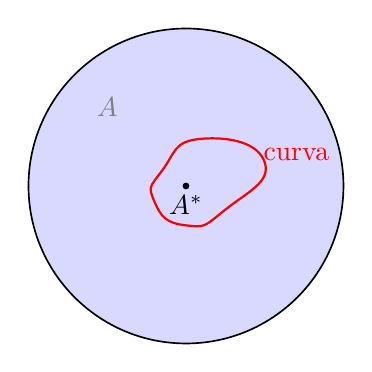
\begin{tikzpicture}
                \draw[fill=blue!15, semithick] (0,0) circle(2);
                \draw[red, thick]
                plot [smooth cycle, tension=1] coordinates {
                    (-0.3,0.2)
                    (0.2,0.6)
                    (1,0.3)
                    (0.5,-0.3)
                    (0,-0.5)
                    (-0.4,-0.2)
                };
    
                \node at (-1,1) {\textcolor{gray}{$A$}};
                \node at (1.4,0.4) {\textcolor{red}{curva}};
                \filldraw[black]  (0,0) circle (1pt) node[below]  {\( A^{*} \) };
            \end{tikzpicture}
        \end{minipage}
    \hspace{1cm}
        \begin{minipage}{0.45\textwidth}
            \centering
            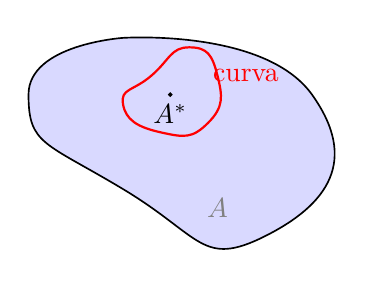
\begin{tikzpicture}[scale=1.2]
                \filldraw[fill=blue!15, semithick]
                    plot[smooth, tension=1.2] coordinates {(1,0.6) (3,0) (2.5,-1.5) (1,-1) (0,0) (1,0.6)};
                    \draw[thick, red]
                    plot [smooth cycle, tension=1] coordinates {
                        (1.3,0.2)
                        (1.7,0.5)
                        (2,0.2)
                        (1.9,-0.3)
                        (1.4,-0.4)
                        (1,-0.1)
                    };
                \node at (2,-1.2) {\textcolor{gray}{$A$}};
                \node[red] at (2.3,0.2) {curva};
                \filldraw[black] (1.5,0) circle (0.5pt) node[below] {\( A^{*} \) };
            \end{tikzpicture}
        \end{minipage}
    \end{center}
    
    \vspace{0.3cm} % Pequeño espacio antes de la etiqueta
    
    \begin{center}
        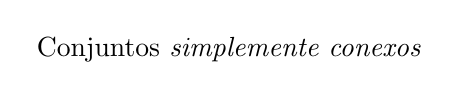
\begin{tikzpicture}
            \node at (1.5,-2) {Conjuntos \emph{simplemente conexos}};
        \end{tikzpicture}
    \end{center}
    
  %  \begin{center}
    %    \begin{tikzpicture}
            % Círculo exterior (azul claro) \draw[fill=blue!15, semithick] (0,0) circle(2);
    %        \draw[fill=blue!15, semithick] (0,0) circle(2);
            
            % Círculo interior (blanco, para el hueco)
  %          \draw[fill=white, semithick] (0,0) circle(0.8);
   %         \draw[red, thick]
     %       plot [smooth cycle, tension=1] coordinates {
      %          (0.7,0.1)
     %           (1,0.5)
     %           (1.4,0.2)
      %          (1.3,-0.3)
     %           (0.9,-0.5)
      %          (0.6,-0.4)
       %         (0.5,-0.1)
        %    };
       %         \node at (-1,1) {\textcolor{gray}{$A$}};
      %          \node at (1,0.9) {\textcolor{red}{curva}};
      %          \filldraw[black] (1,0) circle (0.5pt) node[below] {\( A^{*} \) };;
      %  \end{tikzpicture}
      %  \end{center}
      %  \begin{center}
       %     \begin{tikzpicture}
        %        \node at (1.5,-2) {Conjunto \emph{no simplemente conexo}};
        %    \end{tikzpicture}
       % \end{center}       
  

\begin{definition} \textbf{Conjunto simplemente conexo en $\mathbb{R}^{n}$.} \label{def:conjuntosimpleconexo2}
Sea $A \subseteq \mathbb{R}^{n}$ un conjunto arcoconexo.  Decimos que $A$ es \emph{simplemente conexo} si toda curva continua y cerrada contenida en $A$ puede deformarse continuamente dentro de $A$, manteniendo su punto inicial y final fijos, hasta reducirse a un único punto.
\end{definition}




\includegraphics{tikz/standalone_fig_lazo.pdf}

    
    
    
       
    
    
    
    
    
    
    


\chapter{Campos Escalares y Vectoriales.}
         
\section{Definici\'on de Campos Eectoriales y Escalares}

\begin{obs}
Si en  (\ref{def:FuncMate1})  cambiemos  $A \subseteq \mathbb{R}$ y $B\subseteq \mathbb{R}$ por $A \subseteq \mathbb{R}^{n}$ y $B \subseteq \mathbb{R}^{m}$  obtenemos de manera analoga la siguiente definici\'on.    
\end{obs}





\begin{definition} \textbf{Campos.}
  Un \textit{campo} es una funci\'on   $\campoVec{F}:A\subseteq \mathbb{R}^n \rightarrow B \subseteq \mathbb{R}^m.$    Si $m=1$ lo llamaremos  \textit{ campo escalar }  y  si  $m\geq 2$ lo llamaremos   \textit{ campo vectorial}. Al igual que en (\ref{def:FuncMate1}), a los conjuntos $A$ y $B$  se los llama, respectivamente, \textit{dominio}  y \textit{codominio} del campo $\campoVec{F}$ y  la notaci\'on usual para los mismos  es  $A=\text{Dom}( \campoVec{F})$ y $B=\text{Cod}( \campoVec{F})$.   
  \end{definition}
  
\textbf{Notaci\'on: } En general, la notaci\'on usual  para campos escalares es  con letras imprentas minúsculas y para  los campos vectorials es con letra imprenta mayúscula y negrita. A lo largo del documento mantendremos esta notación. 
  
  \begin{definition} {\textbf{Componentes de un campo vectorial.}}
  Sea   $\campoVec{F}:A\subseteq \mathbb{R}^n \rightarrow B \subseteq \mathbb{R}^m$   un \textit{campo vectorial}, dado $\vect{x}_0 \in A$ se puede pensar a  $\mathbf{F}(\vect{x}_0)$   como la evaluación de $m$ campos escalares en $\vect{x}_0$, 
    es decir,
    \begin{equation*}
        \campoVec{F}(\vect{x}_0)=\big( f_1(\vect{x}_0),..., f_m(\vect{x}_0) \big).
    \end{equation*}
  Para $1 \leq i \leq n$,  el campo escalar $f_i: A\subseteq \mathbb{R}^n \rightarrow  \mathbb{R}$ se llama la \textit{i-\'esima componente} de $\campoVec{F}.$
 \end{definition}
  
  
  \begin{definition}{\textbf{Conjunto Imagen.}}
    Sea  $\campoVec{F}:A\subseteq \mathbb{R}^n \rightarrow B \subseteq \mathbb{R}^m$, se define el \textit{conjunto imagen} de $\mathbf{F}$, y se denota por $ \operatorname{Img}(\mathbf{F})$, a 
    \begin{equation*}
        \operatorname{Img}(\campoVec{F})=\{\mathbf{y}\in\mathbb{R}^m: \mathbf{F}(\mathbf{x})=\mathbf{y}, \mathbf{x} \in A\}.
    \end{equation*}
  \end{definition}
  
  
 
\begin{example} \label{ej:campoEscalar}
La función $d \colon \mathbb{R}^3 \to \mathbb{R}$ definida por $d(x,y,z) = \sqrt{x^2+y^2+z^2}$ es un campo escalar. En este caso, $\operatorname{Dom}(d) = \mathbb{R}^{3}$, $\operatorname{Cod}(d) = \mathbb{R}$ y $\operatorname{Img}(d) = \mathbb{R}_{\geq 0}$.  Para cada  punto $(x,y,z)$  el campo $d$ devuelve la distancia eucl\'idea de dicho punto  al $(0,0,0)$. Por ejemplo,  tomemos el punto $(1,2,2) \in \mathbb{R}^{3}$ entones $\text{d}(1,2,2)= 3$ es la distancia  eucl\'idea  del punto $(1,2,2)$ al punto $(0,0,0).$
Esta relación también se puede visualizar como:
\end{example}
  

\begin{figure}[H]
\centering
\begin{tikzpicture}[scale=1]

% --- Espacio R^3 (dominio) a la izquierda ---
\begin{axis}[
    at={(0,0)},
    anchor=center,        
    width=6cm, height=6cm,
    view={120}{30},
    axis lines=middle,
    axis line style={black!70},
    label style={black!70},
    ticks=none,
    xlabel={$x$}, ylabel={$y$}, zlabel={$z$},
    xmin=0, xmax=3,
    ymin=0, ymax=3,
    zmin=0, zmax=3,
]
% Punto (1,2,2) en R^3
\addplot3[only marks, mark=*, red] coordinates {(1,2,2)};
\node at (axis cs:1,2,2.5) {\textcolor{red}{$(1,2,2)$}}; 
\end{axis}

% --- Título dominio ---
\node at (0,3.3) {Dominio};


% --- Espacio R (codominio) a la derecha como recta numérica ---
% Se usa la punta stealth-stealth para indicar recta infinita en ambos lados
\draw[stealth-stealth, thick, black!70] (5.5,0) -- (10.5,0);

% Título del codominio arriba de la recta
\node at (8,0.5) {Codominio};

% Marca del Origen (0) en la recta numérica
\draw[thick, black!70] (6, -0.1) -- (6, 0.1);
\node at (6, -0.4) {\small $0$};

% --- Pintar la Semirrecta en Azul: Imagen del conjunto [0, +infinito) ---
% Comienza con un corchete en (6,0) y se extiende hasta la punta de la flecha en (10.5,0)
\draw[blue, ultra thick, -stealth] (6,0) -- (10.5,0);

% Corchete izquierdo del intervalo cerrado en el cero
\node[blue] at (6,0) {\textbf{[}};

% Punto Imagen particular d(1,2,2) = 3 (destacado encima de la semirrecta)
\filldraw[blue] (9,0) circle (2pt);
\node at (9,0.4) {\textcolor{blue}{$3$}};


% --- Título general sobre el bloque de la derecha ---
\node at (8,3.3) {Codominio};


% --- Flecha curvada entre los puntos ---
\draw[->, thick, black] (1.8,0.5) .. controls (3.5,2.0) and (4.8,1.7) .. (5.4,0.3);
\node at (3.65,1.8) {\Large $d$};

\end{tikzpicture}
\caption{Visualización de $(1,2,2)$, su imagen $d(1,2,2)=3$ y el conjunto imagen $\operatorname{Img}(d) = \mathbb{R}_{\geq 0}$ resaltado en azul.}
\label{fig:visualizacion_campo_escalar_con_semirrecta}
\end{figure}


\begin{tarea} Hallar todos los puntos $(x,y,z) \in \mathbb{R}^{3}$ tales que  $d(x,y,z)=3$ y dibujarlos. 
\end{tarea}  





\begin{example}
Probar que la transformación lineal $\campoVec{T} \colon \mathbb{R}^2 \to \mathbb{R}^3$ es efectivamente una transformación lineal y calcular su imagen,  siendo $$\campoVec{T}(x,y) = (x+y, x-y, x+y)$$ 
\end{example}

Se deja a cargo del lector probar que $\campoVec{T}$ verifica la \autoref{def:TL}. Para encontrar su imagen, basta con escribir:
\begin{align*}
\campoVec{T}(u_1, u_2) &= (u_1+u_2, u_1-u_2, u_1+u_2) \\
&= (u_1, u_1, u_1) + (u_2, -u_2, u_2) \\
&= u_1(1,1,1) + u_2(1,-1,1), \quad \text{con } u_1, u_2 \in \mathbb{R}.
\end{align*}
Así, la imagen resulta el siguiente plano en $\mathbb{R}^3$ (ver \autoref{def:planoR3}):
\begin{equation*}
\operatorname{Img}(\campoVec{T}) = \{ \vect{x} \in \mathbb{R}^3 \mid \vect{x} = u_1(1,1,1) + u_2(1,-1,1), \; u_1, u_2 \in \mathbb{R} \}.
\end{equation*}
Otra manera equivalente de representar dicho plano es mediante la ecuación:
\[ z = x.\]Finalmente, se puede representar gráficamente el dominio y el codominio.


\begin{figure}[H]
\centering
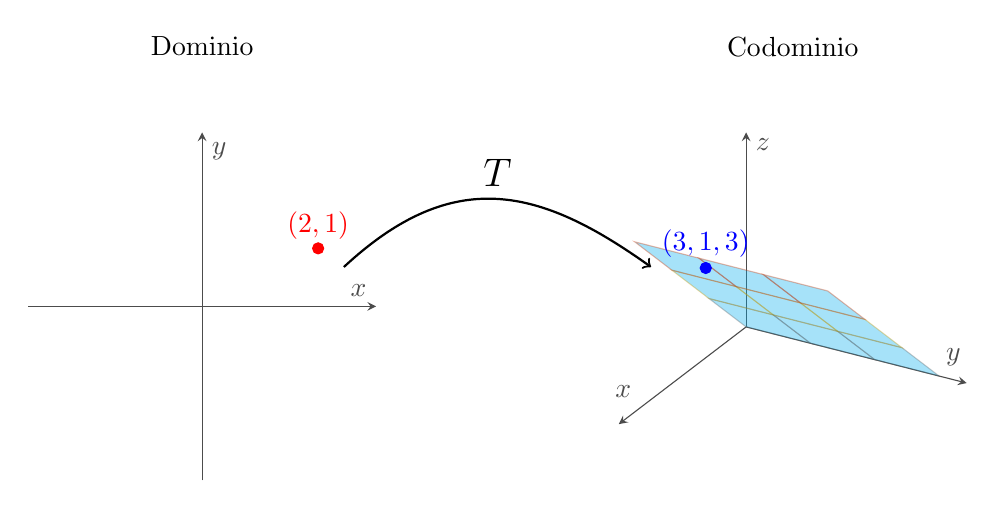
\begin{tikzpicture}[scale=1]

% --- Espacio R^2 (dominio) a la izquierda (Cuatro Cuadrantes) ---
\begin{axis}[
    at={(0,0)},
    anchor=center,        % Cambiado a center para estabilidad geométrica
    width=6cm, height=6cm,
    axis lines=middle,
    axis line style={black!70},
    label style={black!70},
    ticks=none,
    xlabel={$x$}, ylabel={$y$},
    xmin=-3, xmax=3,      
    ymin=-3, ymax=3,      
]
% Punto (2,1) en R^2
\addplot[only marks, mark=*, red] coordinates {(2,1)};
\node at (axis cs:2,1.4) {\textcolor{red}{$(2,1)$}};
\end{axis}

% --- Título dominio ---
\node at (0,3.3) {Dominio};


% --- Espacio R^3 (codominio) a la derecha ---
\begin{axis}[
    at={(7.5cm,0)},       % Alineado horizontalmente a 7.5cm y verticalmente en 0
    anchor=center,        % Anclado al centro para una alineación vertical perfecta
    width=6cm, height=6cm,
    view={120}{30},
    axis lines=middle,
    axis line style={black!70},
    label style={black!70},
    ticks=none,
    xlabel={$x$}, ylabel={$y$}, zlabel={$z$},
    xmin=0, xmax=4,
    ymin=0, ymax=4,
    zmin=0, zmax=4,
]
% --- Dibujo del Plano z = x (Imagen real de T) ---
\addplot3[
    surf,
    fill=cyan,           
    opacity=0.35,        
    draw=cyan!60!black,  
    domain=0:3.5,        
    domain y=0:3.5,      
    samples=4,           
] {x};

% Punto (3,1,3) en R^3
\addplot3[only marks, mark=*, blue] coordinates {(3,1,3)};
\node at (axis cs:3,1,3.5) {\textcolor{blue}{$(3,1,3)$}};
\end{axis}

% --- Título codominio ---
% Reubicado de forma simétrica sobre el eje del codominio
\node at (7.5,3.3) {Codominio};


% --- Flecha curvada entre los puntos (Perfectamente balanceada) ---
% Ahora usa coordenadas relativas al centro de cada bloque, garantizando simetría
\draw[->, thick, black] (1.8,0.5) .. controls (3.2,1.8) and (4.3,1.5) .. (5.7,0.5);
\node at (3.75,1.7) {\Large$\campoVec{T}$};

\end{tikzpicture}
\caption{Visualización de $(2,1)$, su imagen $\campoVec{T}(2,1) = (3,1,3)$ y el plano $z = x$.}
\label{fig:visualizacion_T_con_plano_simetrico}
\end{figure}



       \begin{example}  \label{ej:campoVectorial}
        La función $\mathbf{F}:\mathbb{R}^2 \rightarrow \mathbb{R}^3 \;|\; \mathbf{F}(x,y) = (x+y,x-y,xy)$ es un campo vectorial. 
        En este caso, su dominio es $\mathbb{R}^2 $ y su codominio $\mathbb{R}^3 $.
        
      La imágen de $\mathbf{F}$ se puede hallar con el siguiente planteo:
        \begin{equation*}
          \mathbf{F}(x,y) = (x+y,x-y,xy) = (u,v,w)  .
        \end{equation*}
        Luego, resolviendo el sistema de ecuaciones resultante, se llega a la ecuación
        \begin{equation*}
          w = \frac{u^2}{4}-\frac{v^2}{4},
        \end{equation*} y, por lo tanto, queda 
         \begin{equation}\label{imagF}
          \text{Img}(\mathbf{F})=\left\{ (u,v,w)\in\R^3 \:\Big|\: w=\frac{u^2}{4}-\frac{v^2}{4} \right\}
        \end{equation}  la cual describe  un paraboloide hiperbólico en $\mathbb{R}^3.$ 
       
Visualicemos  la relaci\'on entre  el dominio y la imagen de campo vectorial $\mathbf{F}$ con un caso particular, para ello tomemos el punto $(1,1) \in \mathbb{R}^{2},$  luego $ \mathbf{F}(1,1)=(2,0,1) \in  \text{Img}(\mathbf{F})$
 
 \begin{figure}[H]
  \begin{center}
    \begin{tikzpicture}

      % Plano 2D a la izquierda
      \begin{axis}[
        at={(0,0)},
        anchor=origin,
        axis lines=middle,
        axis line style={black!70},
        label style={black!70},
        ticks=none,
        xlabel={$x$}, ylabel={$y$},
        xmin=-1, xmax=3,
        ymin=-1, ymax=3,
        width=6cm,
        height=6cm,
        title={Dominio}
      ]
        % Punto (1,1)
        \addplot[only marks, mark=*, red] coordinates {(1,1)};
        \node at (axis cs:1.3,0.6) {\textcolor{red}{$(1,1)$}};
      \end{axis}
    
      % Espacio 3D a la derecha, alineado
      \begin{axis}[
        at={(7cm,0.5cm)},
        anchor=origin,
        view={130}{30},
        axis lines=middle,
        axis line style={black!70},
        label style={black!70},
        ticks=none,
        xlabel={$x$}, ylabel={$y$}, zlabel={$z$},
        xmin=-1, xmax=4,
        ymin=-1, ymax=2.5,
        zmin=-1, zmax=3,
        width=7cm,
        height=7cm,
        title={Codominio}
      ]
        % Punto imagen (2,0,1)
        \addplot3[only marks, mark=*, blue] coordinates {(2,0,1)};
        \node at (axis cs:3.5,0.2,1.2) {\textcolor{blue}{$(2,0,1)$}};
      \end{axis}
    
      % Flecha curva más simple
      % Puntos de origen y destino
      \coordinate (A) at (1.3,1.4);
      \coordinate (B) at (3,0);
    
      % Dibujo del arco como flecha
      \draw[->, thick]
        (A) arc[start angle=120, end angle=50, radius=4cm];
    
      % Etiqueta
      \node at (4,1.5) {$\mathbf{T}$};
    \end{tikzpicture}
   \caption {Visualización de $(1,1)$ y $\mathbf{F}(1,1)=(2,0,1)$}
   \end{center}
 \end{figure}
\end{example} 

\begin{tarea} Graficar   $ \text{Img}(\campoVec{F})  \: (\ref{imagF}).$
\end{tarea}

    

    
  
\section{Gráficas}
 Si en la \autoref{def:grafm1} cambiamos  $A \subseteq \mathbb{R}$ por $A \subseteq \mathbb{R}^{n}$  y  $B \subseteq \mathbb{R}$ por $B \subseteq \mathbb{R}^{m}$ obtenemos de manera an\'aloga la siguiente definici\'on.    


\begin{definition}\textbf{Gráfica de un campo vectorial}
\label{def:grafica_campo_vec}
Sea $\campoVec{F} \colon A \subseteq \mathbb{R}^n \to \mathbb{R}^m$ un campo vectorial,  se define la \textit{gráfica de $\campoVec{F}$}, y se denota como $\operatorname{Graf}(\mathbf{f})$, al conjunto:
\[ 
\operatorname{Graf}(\campoVec{F}) = \{ (\mathbf{x}, \mathbf{y}) \in \mathbb{R}^{n} \times \mathbb{R}^{m} \mid \mathbf{x} \in A \land \mathbf{y} = \campoVec{F}(\mathbf{x}) \} 
\]
\end{definition}

\begin{obs} Siendo $\campoVec{F} \colon A \subseteq \mathbb{R}^n \to \mathbb{R}^m$ un campo vectorial entonces  desde la Definicón \ref{def:grafica_campo_vec} se desprende de manera inmediata que 
 \[
\operatorname{Graf}(\campoVec{F})   \subseteq  \mathbb{R}^{n+m}.
 \]
\end{obs}
Para el caso particular de un campo escalar obtenemos la siguiente definición
\begin{definition}\textbf{Gráfica de un campo escalar.} 
 \label{def:grafica}
 Sea \( f: A  \subseteq  \mathbb{R}^n \to  \mathbb{R}\),  se define la \textit{gráfica de $f$}, y se nota $\text{Graf}(f)$,  a
 \[
\operatorname{Graf}(f)=\{(\mathbf{x}, y) \in  \mathbb{R}^{n} \times \mathbb{R}  \;|\; \mathbf{x} \in A \land  y = f(\mathbf{x}) \}
 \]
\end{definition}


\begin{obs}  Siendo \( f: A  \subseteq  \mathbb{R}^n \to  \mathbb{R}\) un campo escalar   entonces  desde la Definicón \ref{def:grafica}  se desprende que  $$\text{Graf}(f) \subseteq  \mathbb{R}^{n+1}.$$  Con el objetivo de poder dibujar,  nos detendremos especialmente en el caso de gr\'aficas de  campos  $f: A\subseteq \mathbb{R}^2 \rightarrow \mathbb{R},$ cuya definici\'on es,  
 \[
\operatorname{Graf}(f)=\{(x,y,z)\in \mathbb{R}^3 \;|\;(x,y)\in A \land z=f(x,y) \}.
 \]
\end{obs}

 




         

            
 \section{Conjuntos de nivel}
  %---------------------------------------------------------def trazal---------------------------------------------------------------
    
%\begin{definition}   \textbf{Hiperplano.}   Un \emph{hiperplano} en \(\mathbb{R}^n\) es un subconjunto afín de dimensión \(n-1\). Más concretamente, dados un %vector no nulo \(\mathbf{a}\in\mathbb{R}^n\) y un escalar \(b\in\mathbb{R}\), el hiperplano asociado se define como
%\[
%H = \{\,\mathbf x\in\mathbb{R}^n : \langle \mathbf{a},\mathbf{x}\rangle = b\},
%\]
%donde \(\langle \mathbf{a},\mathbf{x}\rangle = a_1 x_1 + a_2 x_2 + \cdots + a_n x_n\) es el producto escalar en \(\mathbb{R}^n\).  En \(\mathbb{R}^3\) los %hiperplanos son los planos, ver definici\'on (\ref{plano}).
%\end{definition} 
    

%\begin{definition}\textbf{Traza.} 
%Se llama \emph{traza} de un conjunto \( S \subseteq \mathbb{R}^n \) a la intersección de \( S \) con un hiperplano \( H \subseteq \mathbb{R}^n \). 
%\end{definition}


%A continuaci\'on, definiremos unas Trazas particulares llamadas  \textbf{Conjunto de nivel}  y  \textbf{Cortes transversales} para conjuntos dados por g\'raficas de %funciones ( \ref{def:grafica})  


%---------------------------------------------------------def conjunto de nivel----------------------------------------------------
\begin{definition} \textbf{Conjunto de nivel.} 
    \label{def:conjunto de nivel}     
    Sea $f: U  \subseteq  \mathbb{R}^n \rightarrow \mathbb{R}$ y sea $c \in \mathbb{R}$, se define  \emph{el conjunto de nivel de $f$ de nivel}  $c$, y se nota $C(c,f)$,  como  
    \[
    C(c,f)=\{ \mathbf{x} \in U \;|\; f (\mathbf{x})=c \}.
     \]
 Es decir,  $C(c,f)$ es el conjunto de puntos $\vect{x}\in\ U$ para los cuales $f(x)=c$, o dicho de otra manera,  $C(c,f)$ es la preimagen de $c$ por $f$.   Llamaremos a los conjuntos de nivel por \emph{ curva de nivel}  o   \emph{superficie de nivel}, si $n=2$ o si $n=3$ respectivamente.   
\end{definition}


\begin{obs}  Si $f: U \subseteq \mathbb{R}^n \rightarrow \mathbb{R}$ entonces $C(c,f)   \subseteq  \mathbb{R}^{n}.$   Con el objetivo de poder dibujar,  nos detendremos en los casos $n=2$ y $n=3$  cuya definici\'on se desprende automaticamente  de la definici\'on  (\ref{def:conjunto de nivel}), es decir, 
 \begin{align}\label{def:conjunto de nive perticular} 
    C(c,f)&=\{ (x,y) \in U \;|\; f (x,y)=c \} \mbox{ si } n=2. \\
     C(c,f)&=\{ (x,y,z) \in U \;|\; f (x,y,z)=c \} \mbox{ si } n=3.
  \end{align} 
\end{obs}


\begin{definition} \textbf{Corte transversal.}   Sea $f: U  \subseteq  \mathbb{R}^2 \rightarrow \mathbb{R}$ y sea $a \in \mathbb{R}$, se define  \emph{el corte tranversal $f$}  con el plano vertical $x=a$, al conjunto
    \[
    \{   (x,y,z) \in \mathbb{R}^{3} \;|\; x=a \; ;\;   f (a,y)=z \},
     \] analogamente,  si $b \in \mathbb{R}$, se define  \emph{el corte tranversal $f$}  con el plano vertical $y=b$, al conjunto
    \[
    \{   (x,y,z) \in \mathbb{R}^{3} \;|\; y=b \; ;\;   f (x,b)=z \}.
     \]
\end{definition}


%----------------------------------------------------------ejemplos--------------------------------------------------------------

\begin{example}\label{example:ex1graf}   Sea  el campo  $f: \mathbb{R}^{2} \rightarrow \mathbb{R} \:|\:  f(x,y)=x^2+y^2.$ Hallar y graficar,  los conjuntos de nivel de $f$ y los cortes transversales  de  $\text{Graf}(f)$ con los planos de ecuaciones $x=0$ y $y=0$ . Hacer un dibujo de  $\text{Graf}(f)$.

        
Dado $c \in \mathbb{R}$, por (\ref{def:conjunto de nive perticular}), sabemos que 
     $$C(c,f)=\{(x,y) \in (\mathbb{R}^2 \;|\;   x^2+y^2  =c \}.$$

Tomemos, para ilustrar,  $c=0$, $c=1$ y $c=4$, 
    % quedando (ver (\ref{circ})) 
\begin{align*}   
C(0,f)&=\{(x,y) \in U \;|\; x^2+y^2=0 \}=\{(0,0) \} \\
C(1,f)&=\{(x,y) \in U \;|\; x^2+y^2=1 \} \\
C(4,f)&=\{(x,y) \in U \;|\; x^2+y^2=4 \}.
\end{align*}    
    

 \begin{figure}[H]  
\begin{center}
    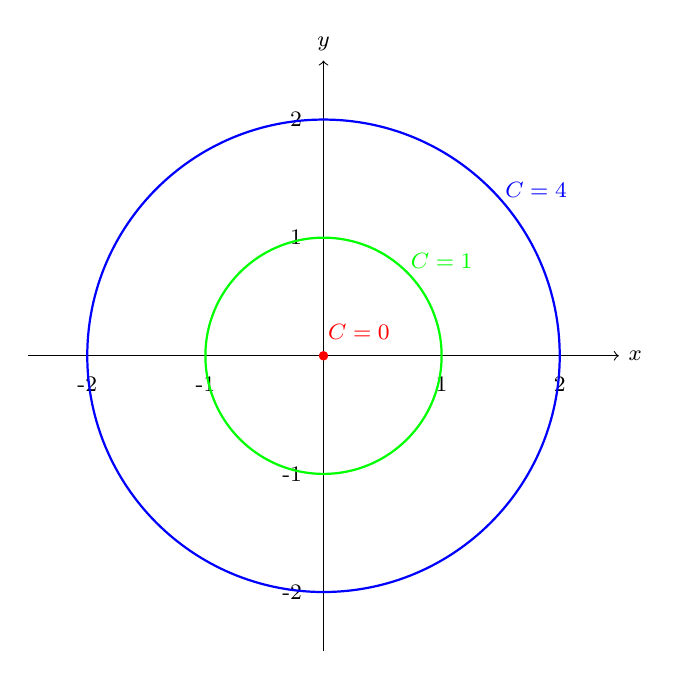
\begin{tikzpicture}[scale=1.5]
        % Dibujar ejes coordenados con números
        \draw[->] (-2.5,0) -- (2.5,0) node[right] {\footnotesize $x$};
        \draw[->] (0,-2.5) -- (0,2.5) node[above] {\footnotesize $y$};
        
        % Marcas y etiquetas en los ejes
        \foreach \x in {-2,-1,1,2}
            \draw (\x,0.1) -- (\x,-0.1) node[below] {\footnotesize \x};
        \foreach \y in {-2,-1,1,2}
            \draw (0.1,\y) -- (-0.1,\y) node[left] {\footnotesize \y};
        
        % Dibujar los círculos de nivel en sentido antihorario
        \draw[thick, green] (0,0) circle (1);
        \draw[thick, blue] (0,0) circle (2);

        
        % Etiquetas de los conjuntos de nivel
        \node[green] at (1,0.8) {\footnotesize $C=1$};
        \node[blue] at (1.8,1.4) {\footnotesize$C=4$};
        \node[red] at (0.3,0.2) {\footnotesize $C=0$};
        
        % Punto en el origen
        \filldraw[red] (0,0) circle (1pt);
    \end{tikzpicture}
\end{center}
  \caption{En rojo,  verde y azul  los conjuntos $C(0,f)$, $C(1,f)$ y $C(4,f)$, respectivamente.}
        %\label{fig:unitCircle1} 
   \end{figure}

    
    En general, podemos escribir a los conjuntos de nivel de $f$ como: 
       \[
            C(c,f)=
            \begin{dcases}
               x^2+y^2=c  &  c>0 \\
    (0,0)  & c=0\\
    \varnothing  & c<0.\\
            \end{dcases}
        \]

 Cada punto \( (x,y)\in  C(c,f)\)  se eleva al espacio como \((x,y,c)\),  colocándolo en el plano horizontal \(z = c\), generando un conjunto en el espacio.  El total de dichos conjuntos en distintos niveles \(c\) reconstruye una aproximación de la gráfica de $f$. En nuestro caso, podemos pensar a estos conjuntos como cortes entre la $\text{Graf}(f)$  y los planos horizontales $z=0$, $z=1$ y $z=4$ en $\mathbb{R}^{3}$, obteniendo

 \begin{figure}[H] 
\begin{center}
        %\begin{tabular}{cc}
            \begin{minipage}{0.45\textwidth}
              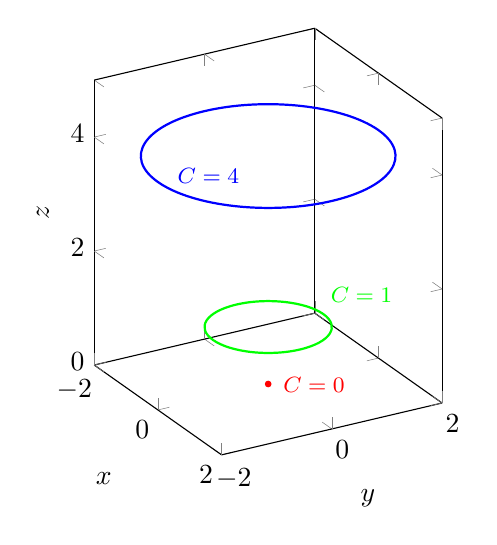
\begin{tikzpicture}
                  \begin{axis}[
                    view={60}{20},
                      xlabel={$x$},
                      ylabel={$y$},
                       zlabel={$z$},
                        xmin=-2, xmax=2,
                        ymin=-2, ymax=2,
                        zmin=0, zmax=5,
                       samples=50,
                       width=6cm,
                        height=7cm,
                        colormap/viridis
                    ]
                       \draw[thick, green] (0,0,1) circle (1);
                        \draw[thick, blue] (0,0,4) circle (2);
                        \node[green] at (1.2,1,1.8) {\footnotesize $C=1$};
                        \node[blue] at (0.2,-1.2,4) {\footnotesize $C=4$};
                        \node[red] at (0.4,0.6) {\footnotesize $C=0$};
                        \filldraw[red] (0,0) circle (1pt);
                    \end{axis}
                \end{tikzpicture}
            \end{minipage}
\end{center}
 \caption{En rojo,  verde y azul  los cortes de $\text{Graf}(f)$  con los planos horizontales $z=0$, $z=1$ y $z=4$, respectivamente.}
        %\label{fig:unitCircle1} 
  \end{figure}


Tomemos el corte transversal con el plano vertival $x=0$ y se deja al lector analizar el corte  $y=0.$  Para ello, observemos que, si $x=0$

$$z=f(0,y)=y^2.$$

\begin{figure}[H]
\begin{center}
    \begin{tikzpicture}
        % Ejes coordenados
        \draw[->] (-2.5,0) -- (2.5,0) node[right] {\footnotesize $y$};
        \draw[->] (0,-0.5) -- (0,4.5) node[above] {\footnotesize $z$};

        % Marcas en los ejes
        \foreach \x in {-2,-1,1,2}
            \draw (\x,0.1) -- (\x,-0.1) node[below] {\footnotesize \x};
        \foreach \y in {1,2,3,4}
            \draw (0.1,\y) -- (-0.1,\y) node[left] {\footnotesize \y};

        % Gráfica de f(y) = y^2
        \draw[domain=-2:2, smooth, variable=\y, blue, thick] 
            plot ({\y}, {\y*\y});

        % Etiqueta de la curva
        \node[blue] at (2, 1.6) {$z = y^2$};
    \end{tikzpicture}
\end{center}
 \caption{En  azul la relaci\'on $z=y^{2}$ y $x=0.$  }
        %\label{fig:unitCircle1} 
  \end{figure}

 Por \'ultimo, uniendo la informaci\'on hasta aca conseguida, tenemos que la gr\'afica de $f$ es

 \begin{figure}[H]
\begin{center}
    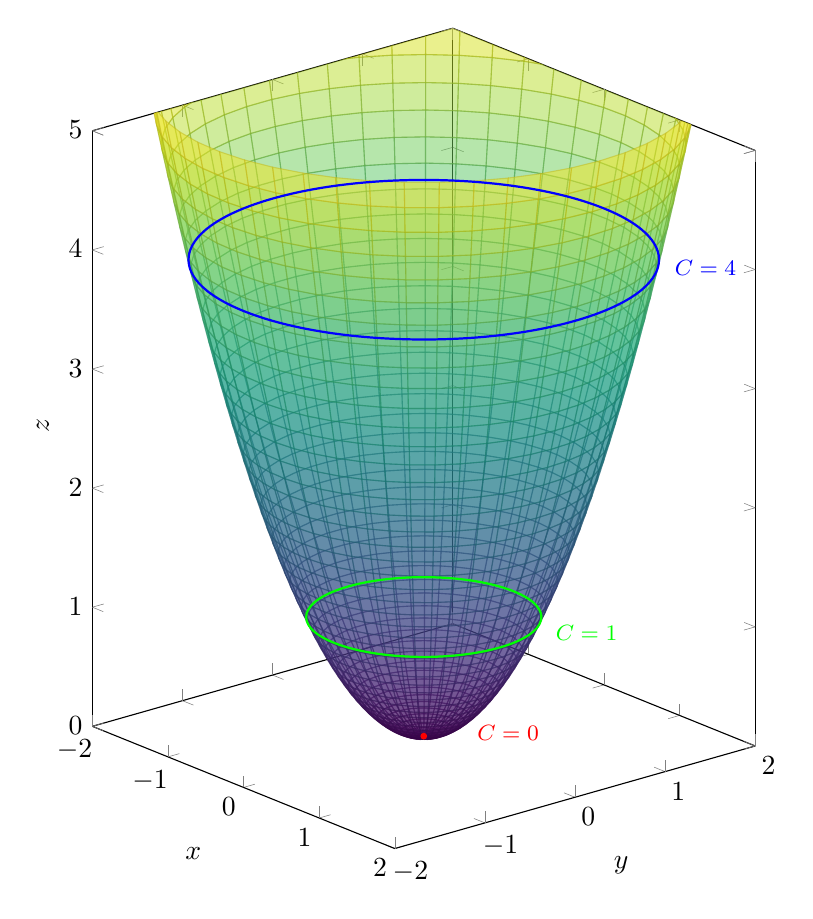
\begin{tikzpicture}
        \begin{axis}[
            view={50}{15},
            xlabel={$x$},
            ylabel={$y$},
            zlabel={$z$},
            xmin=-2, xmax=2,
            ymin=-2, ymax=2,
            zmin=0, zmax=5,  % Extender el eje z hasta 5
            samples=50,
            width=10cm,
            height=12cm,
            colormap/viridis
        ]
            \addplot3 [
                surf, opacity=0.5, draw=none, 
                restrict z to domain=0:5.6,
                data cs=polar, 
                domain=0:360, 
                y domain=0:{sqrt(5.9)}  % Ajustar el dominio radial
            ] 
            (x, y, y^2);
                % Dibujar los círculos de nivel en sentido antihorario
        \draw[thick, green] (0,0,1) circle (1);
        \draw[thick, blue] (0,0,4) circle (2);

     
        
        % Etiquetas de los conjuntos de nivel
        \node[green] at (1.2,0.8,1) {\footnotesize $C=1$};
        \node[blue] at (1.7,1.7,4) {\footnotesize $C=4$};
        \node[red] at (0.4,0.6) {\footnotesize $C=0$};
        
        % Punto en el origen
        \filldraw[red] (0,0) circle (1pt);
        \end{axis}
    \end{tikzpicture}
\end{center}
 \caption{Gr\'afica de la funci\'on $f$. }
        %\label{fig:unitCircle1} 
  \end{figure}
\end{example}


%\newpage     
    
\begin{example}\label{example:ej2graf} Para  el campo  $g: \mathbb{R}^{2} \rightarrow \mathbb{R} \;|\; g(x,y) = \sqrt{x^2+y^2},$  hallar y graficar,  los conjuntos de nivel de $g$ y los cortes transversales  de  $\text{Graf}(g)$ con los planos de ecuaciones $x=0$ y $y=0$ .  Hacer un dibujo de  $\text{Graf}(f)$.  




  
Dado $c \in \mathbb{R}$, por (\ref{def:conjunto de nive perticular}), sabemos que   $$C(c,g)=\{(x,y) \in U \;|\;   \sqrt{x^2+y^2}  =c \}.$$
    
Tomemos, para ilustrar,  $c=0$, $c=1$ y $c=2$, 
    % quedando (ver (\ref{circ})) 
    \[
        C(0,g)=\{(x,y) \in U \;|\; \sqrt{x^2+y^2}=0 \}
        \]
         \[
        C(1,g)=\{(x,y) \in U \;|\; \sqrt{x^2+y^2}=1 \}
        \]
         \[
        C(2,g)=\{(x,y) \in U \;|\; \sqrt{x^2+y^2}=2 \}.
         \]
    
    
  
    
\begin{figure}[H]
     \begin{center}
        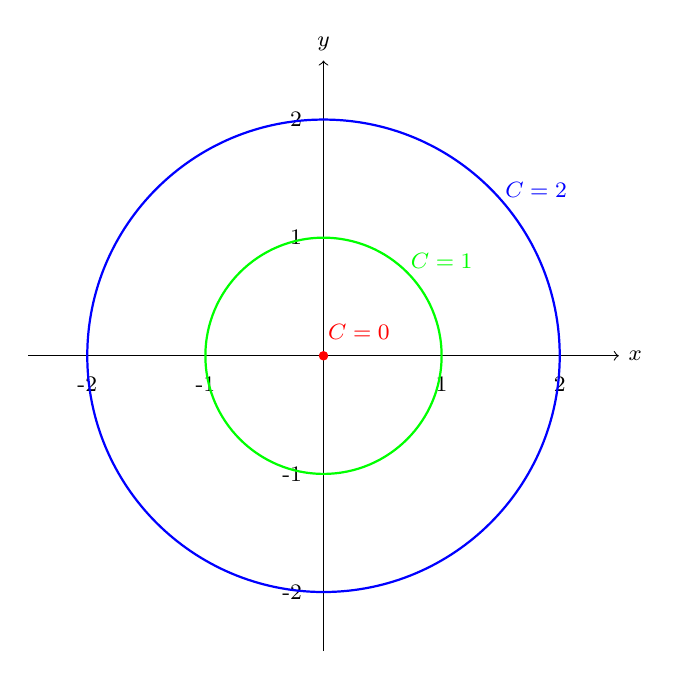
\begin{tikzpicture}[scale=1.5]
            % Dibujar ejes coordenados con números
            \draw[->] (-2.5,0) -- (2.5,0) node[right] {\footnotesize $x$};
            \draw[->] (0,-2.5) -- (0,2.5) node[above] {\footnotesize $y$};
            
            % Marcas y etiquetas en los ejes
            \foreach \x in {-2,-1,1,2}
                \draw (\x,0.1) -- (\x,-0.1) node[below] {\footnotesize \x};
            \foreach \y in {-2,-1,1,2}
                \draw (0.1,\y) -- (-0.1,\y) node[left] {\footnotesize \y};
            
            % Dibujar los círculos de nivel en sentido antihorario
            \draw[thick, green] (0,0) circle (1);
            \draw[thick, blue] (0,0) circle (2);
    
            
            % Etiquetas de los conjuntos de nivel
            \node[green] at (1,0.8) {\footnotesize $C=1$};
            \node[blue] at (1.8,1.4) {\footnotesize $C=2$};
            \node[red] at (0.3,0.2) {\footnotesize $C=0$};
            
            % Punto en el origen
            \filldraw[red] (0,0) circle (1pt);
        \end{tikzpicture}
  \end{center}
  \caption{En rojo,  verde y azul  los conjuntos $C(0,g)$, $C(1,g)$ y $C(4,g)$, respectivamente.}
        %\label{fig:unitCircle1} 
   \end{figure}
    
   En general, podemos escribir a los conjuntos de nivel de $g$ como:
       \[
            C(c,f)=
            \begin{dcases}
            \sqrt{ x^2+y^2}=c  &  c>0 \\
    (0,0)  & c=0\\
    \varnothing  & c<0.\\
            \end{dcases}
        \]
   

Analogamente al ejemplo anterior, podemos "elevar"  los  conjuntos $ C(c,f)$  a "altura"  $z=c$ y dibujarlos en  $\mathbb{R}^{3}$
 \begin{figure}[H]
\begin{center}
 \tikzsetnextfilename{Conjuntos-de-nivel-cono}  
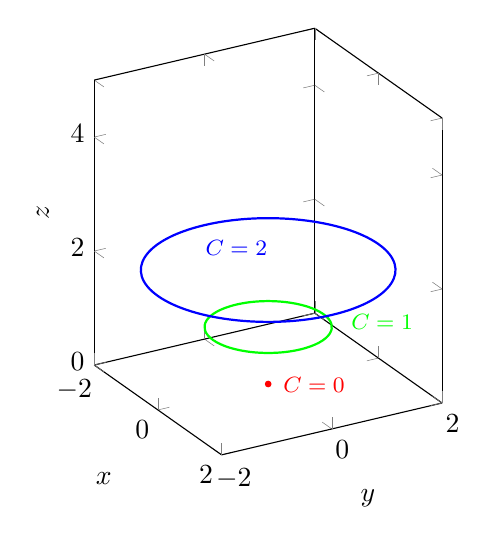
\begin{tikzpicture} 
                        \begin{axis}[
                        view={60}{20},
                        xlabel={$x$},
                        ylabel={$y$},
                        zlabel={$z$},
                        xmin=-2, xmax=2,
                        ymin=-2, ymax=2,
                        zmin=0, zmax=5,
                        samples=50,
                        width=6cm,
                        height=7cm,
                        colormap/viridis
                    ]
                    \draw[thick, green] (0,0,1) circle (1);
                    \draw[thick, blue] (0,0,2) circle (2);
            
                 
                    
                    % Etiquetas de los conjuntos de nivel
                    \node[green] at (1.5,1.2,1.4) {\footnotesize $C=1$};
                    \node[blue] at (-1,0,2) {\footnotesize $C=2$};
                    \node[red] at (0.4,0.6) {\footnotesize $C=0$};
                    
                    % Punto en el origen
                    \filldraw[red] (0,0) circle (1pt);
                    \end{axis}
                \end{tikzpicture}
        \end{center}
\caption{En rojo,  verde y azul  los cortes de la $\text{Graf}(f)$  con los planos horizontales $z=0$, $z=1$ y $z=2$, respectivamente.}
        %\label{fig:unitCircle1} 
  \end{figure}

%%%%%%%%%%%%%%%%%%%%%%%%%%%%%%%%%%%%%%%%%%%%%%%%%
Tomemos el corte transversal con el plano vertival $x=0$ y se deja al lector analizar el corte  $y=0.$  Para ello, observemos que, si $x=0$
$$z= f(0,y)=|y|$$

 \begin{figure}[H]
\begin{center}
    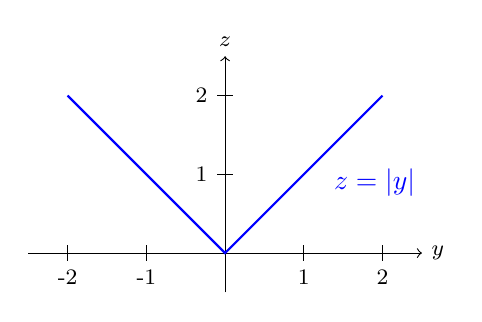
\begin{tikzpicture}
        % Ejes coordenados
        \draw[->] (-2.5,0) -- (2.5,0) node[right] {\footnotesize $y$};
        \draw[->] (0,-0.5) -- (0,2.5) node[above] {\footnotesize $z$};

        % Marcas en los ejes
        \foreach \x in {-2,-1,1,2}
            \draw (\x,0.1) -- (\x,-0.1) node[below] {\footnotesize \x};
        \foreach \y in {1,2}
            \draw (0.1,\y) -- (-0.1,\y) node[left] {\footnotesize \y};

        % Gráfica de f(y) = |y|
        \draw[thick, blue] (-2,2) -- (0,0) -- (2,2);

        % Etiqueta de la curva
        \node[blue, below, xshift=0.6cm] at (1.3, 1.2) {$z = |y|$};
    \end{tikzpicture}
\end{center}
 \caption{En   azul la relaci\'on $z=|y| $ y $x=0.$  }
        %\label{fig:unitCircle1} 
  \end{figure}


 Por \'ultimo, uniendo la informaci\'on hasta aca conseguida, tenemos que la gr\'afica de $g$ es
   
 \begin{figure}[H]
       \begin{center}
         %\tikzsetnextfilename 
          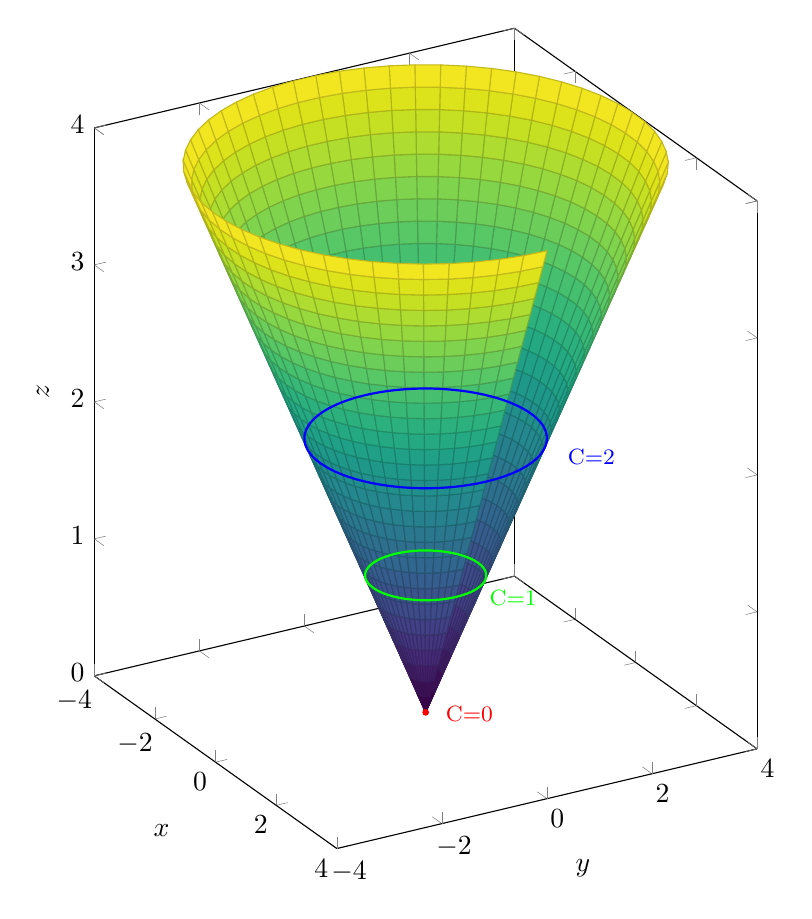
\begin{tikzpicture} 
                \begin{axis}[
                        view={60}{20},
                        xlabel=$x$,
                        ylabel=$y$,
                        zlabel=$z$,
                        xmin=-4,
                        ymin=-4,
                        zmin=0,
                        xmax=4,
                        ymax=4,
                        zmax=4,
                        samples=50,
                        width=10cm,
                        height=12cm,
                        colormap/viridis,
                    ]
                    \addplot3[
                surf,
                domain=0:4,
                y domain=0:360,
                samples=30,
                samples y=60
            ]
            ({x*cos(y)},{x*sin(y)},{x}); % Parámetrico: x = r cos(θ), y = r sin(θ), z = r
               % Dibujar los círculos de nivel en sentido antihorario
            \draw[thick, green] (0,0,1) circle (1);
            \draw[thick, blue] (0,0,2) circle (2);
    
         
            
            % Etiquetas de los conjuntos de nivel
            \node[green] at (1.5,0.8,1) {\footnotesize C=1};
            \node[blue] at (2,2,2) {\footnotesize C=2};
            \node[red] at (0.4,0.6) {\footnotesize C=0};
            
            % Punto en el origen
            \filldraw[red] (0,0) circle (1pt);
                \end{axis}
                
            \end{tikzpicture}
            
        \end{center}
   \caption{Gr\'afica de la funci\'on $g$.  }
        %\label{fig:unitCircle1} 
  \end{figure}
\end{example}
    
    
    \begin{obs} Dibujar todos los puntos en $\mathbb{R}^{3}$ tales que \( z^2 = x^2 + y^2 \).  si despejamos \( z \) obtenemos dos expresiones:
        \[
        z = \sqrt{x^2 + y^2} ,
        \quad
        z = -\sqrt{x^2 + y^2}.
        \]
        Definimos entonces las funciones:
        \[
        f_1 : \mathbb{R}^2 \to [0,+\infty), \quad f_1(x,y) = \sqrt{x^2 + y^2},
        \]
        \[
        f_2 : \mathbb{R}^2 \to (-\infty,0], \quad f_2(x,y) = -\sqrt{x^2 + y^2}.
        \]
        
        Así, los conjuntos de nivel de \( f_1 \) y \( f_2 \) son:
        \[
        C(c,f_1)=
        \begin{dcases}
        x^2+y^2=c  &  c>0 \\
        (0,0)  & c=0\\
        \varnothing  & c<0\\
        \end{dcases}
        \]
        \[
        C(c,f_2)=
        \begin{dcases}
        x^2+y^2=c  &  c<0 \\
        (0,0)  & c=0\\
        \varnothing  & c>0\\
        \end{dcases}
        \]

        De esta manera, considerando la definición de gráfica de una función, podemos representar en \(\mathbb{R}^3\) las gráficas de \( f_1 \) y \( f_2 \), que juntas forman el cono dado por la ecuación \( z^2 = x^2 + y^2 \).
        
        \begin{center}
            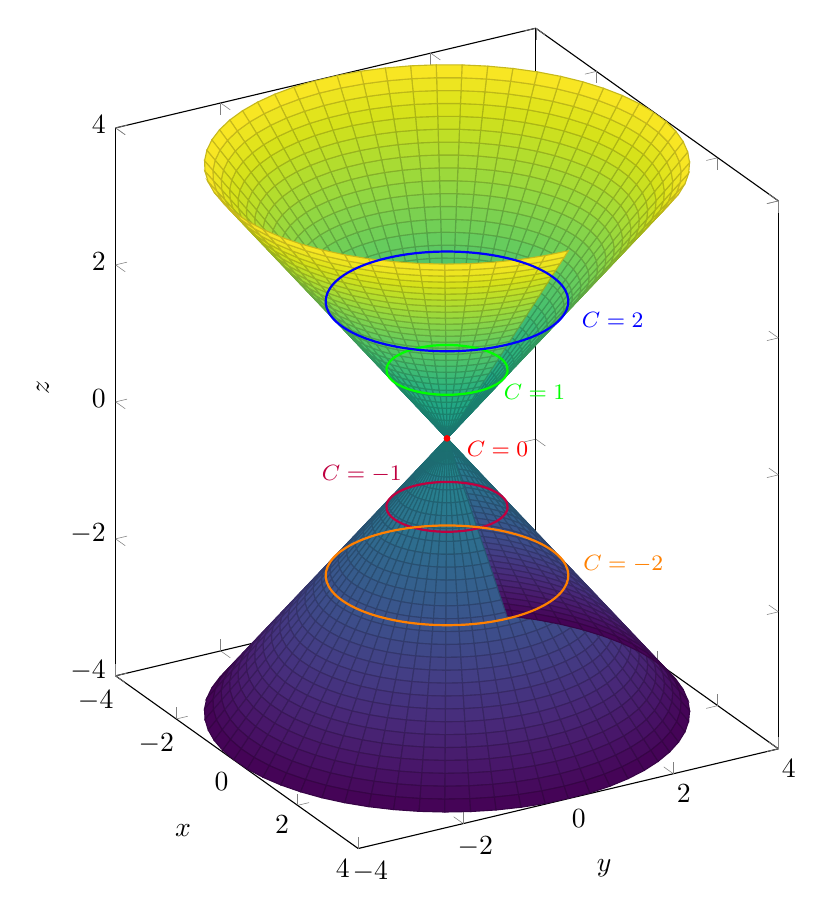
\begin{tikzpicture}
                \begin{axis}[
                        view={60}{20},
                        xlabel=$x$,
                        ylabel=$y$,
                        zlabel=$z$,
                        xmin=-4,
                        ymin=-4,
                        zmin=-4,
                        xmax=4,
                        ymax=4,
                        zmax=4,
                        samples=50,
                        width=10cm,
                        height=12cm,
                        colormap/viridis,
                    ]
                    % Cono superior
                    \addplot3[
                        surf,
                        domain=0:4,
                        y domain=0:360,
                        samples=30,
                        samples y=60
                    ]
                    ({x*cos(y)},{x*sin(y)},{x});
                    
                    % Cono inferior
                    \addplot3[
                        surf,
                        domain=0:4,
                        y domain=0:360,
                        samples=30,
                        samples y=60
                    ]
                    ({x*cos(y)},{x*sin(y)},{-x});
        
                    % Dibujar los círculos de nivel en sentido antihorario
                    \draw[thick, green] (0,0,1) circle (1);
                    \draw[thick, blue] (0,0,2) circle (2);
                    \draw[thick, purple] (0,0,-1) circle (1);
                    \draw[thick, orange] (0,0,-2) circle (2);
        
                    % Etiquetas de los conjuntos de nivel
                    \node[green] at (1.5,0.8,1) {\footnotesize $C=1$};
                    \node[blue] at (2,2,2) {\footnotesize $C=2$};
                    \node[purple] at (1,-2.2,0.2) {\footnotesize $C=-1$};
                    \node[orange] at (2,2.2,-1.6) {\footnotesize $C=-2$};
                    \node[red] at (0.8,0.5,0) {\footnotesize $C=0$};
                    
                    % Punto en el origen
                    \filldraw[red] (0,0,0) circle (1pt);
                \end{axis}
            \end{tikzpicture}
        \end{center}
        \end{obs}


  

 







       
  
  
         
 \section{L\'imite y continuidad de Campos Escalares y Vectoriales}
  \label{sec:limites}
\begin{definition} \textbf{L\'imite.} \label{def:limite_normas} 
Sean $\campoVec{F}:A \subseteq \Rn{n} \to \Rn{m}$ una funci\'on, $L \in \Rn{m}$ y $\vect{x}_0$ un punto de acumulaci\'on de $A$. Decimos que \emph{el l\'imite de $\campoVec{F}$ para $\vect{x}$ tendiendo a $\vect{x}_0$ es $L$} o que \emph{$\campoVec{F}$ tiende a $L$ cuando $\vect{x}$ tiende a $\vect{x}_0$} si 
\[ 
\forall \varepsilon > 0, \, \exists \, \delta > 0 \quad \text{tal que} \quad 0 < \lVert \vect{x} - \vect{x}_0 \rVert < \delta \land \vect{x} \in A \implies \lVert \campoVec{F}(\vect{x}) - L \rVert < \varepsilon. 
\] 
En este caso, utilizamos la notaci\'on 
\[ 
\campoVec{F}(\vect{x}) \xrightarrow[\vect{x} \to \vect{x}_0]{} L \quad \text{o} \quad \lim_{\vect{x} \to \vect{x}_0} \campoVec{F}(\vect{x}) = L. 
\] 
\end{definition}



\begin{obs} \label{obs:entornos_distancias}
A veces es útil expresar la misma definición en t\'erminos de entornos (bolas), lo cual equivale a utilizar funciones de distancia:
\[ 
\forall \varepsilon > 0, \, \exists \, \delta > 0 \quad \text{tal que} \quad \vect{x} \in B_{\delta}^*(\vect{x}_0) \cap A \implies \campoVec{F}(\vect{x}) \in B_{\varepsilon}(L). 
\] 
Recordemos que la pertenencia a la bola reducida $\vect{x} \in B_{\delta}^*(\vect{x}_0)$ equivale matem\'aticamente a la desigualdad de distancias $0 < \dis_n(\vect{x},\vect{x}_0) < \delta$.
\end{obs}

\begin{obs} \label{obs:campo_escalar} 
Si la funci\'on es un \emph{campo escalar} (es decir, $m = 1$), se suele denotar a la funci\'on con la letra min\'uscula $f$ y a su l\'imite con la letra $l \in \mathbb{R}$. En este caso, la condici\'on sobre el codominio $\lVert \campoVec{F}(\vect{x}) - L \rVert < \varepsilon$ se reduce al valor absoluto tradicional, escribi\'endose la definici\'on como:
\[ 
\forall \varepsilon > 0, \, \exists \, \delta > 0 \quad \text{tal que} \quad 0 < \lVert \vect{x} - \vect{x}_0 \rVert < \delta \land \vect{x} \in A \implies \abs{f(\vect{x}) - l} < \varepsilon. 
\] 
\end{obs}


\begin{theorem}\textbf{Unicidad del l\'imite.} \label{teo:unicidad_limite} Sean $\mathbf{F}:A  \subseteq  \Rn{n} \to \Rn{m}$ una funci\'on, $\mathbf{x}_0$ un punto de acumulaci\'on de $A$ y $\mathbf{L}_1, \mathbf{L}_2 \in \Rn{m}$ tales que 
\[
 \mathbf{F}(\mathbf{x}) \xrightarrow[\mathbf{x} \to \mathbf{x}_0]{} \mathbf{L}_1 \quad \wedge \quad \mathbf{F}(\mathbf{x}) \xrightarrow[\mathbf{x} \to \mathbf{x}_0]{} \mathbf{L}_2,
\]
entonces  $\mathbf{L}_1 = \mathbf{L}_2$.
\end{theorem}


\begin{proof}  Como 
\[
 \mathbf{F}(\mathbf{x}) \xrightarrow[\mathbf{x} \to \mathbf{x}_0]{} \mathbf{L}_1,
\]
dado $\varepsilon > 0$ existe alg\'un $\delta_1 > 0$ tal que cada punto $\mathbf{x} \in B_{\delta_1}^*(\mathbf{x}_0) \cap A$ se aplica a trav\'es de $\mathbf{F}$ en alg\'un punto de la bola de centro $\mathbf{L}_1$ y radio $\varepsilon$.

\def\Ro{2.0}
\def\Rb{1.0}
\def\Ra{3.0}
\def\sep{1.0*\Ro}

\input{figs/fig1}

De la misma manera, como 
\[
 \mathbf{F}(\mathbf{\mathbf{x}}) \xrightarrow[\mathbf{\mathbf{x}} \to \mathbf{\mathbf{x}}_0]{} \mathbf{L}_2,
\]
dado $\varepsilon > 0$ existe alg\'un $\delta_2 > 0$ tal que cada punto $\mathbf{\mathbf{x}} \in B_{\delta_2}^*(\mathbf{\mathbf{x}}_0) \cap A$ se aplica a trav\'es de $\mathbf{F}$ en alg\'un punto de la bola de centro $\mathbf{L}_2$ y radio $\varepsilon$.

\input{figs/fig2}

Si suponemos que $\mathbf{L}_1 \ne \mathbf{L}_2$, por propiedad de la distancia es $\dis(\mathbf{L}_1,\mathbf{L}_2) > 0$ y podemos elegir 
\[
 \varepsilon = \frac{\dis{(\mathbf{L}_1,\mathbf{L}_2)}}{2}.
\]
Para este valor de $\varepsilon$ podemos encontrar un punto $\mathbf{\mathbf{x}}$ que se aplica por $\mathbf{F}$ en alg\'un punto de la bola de centro $\mathbf{L}_1$ y radio $\varepsilon$ \textbf{y tambi\'en} se aplica por $\mathbf{F}$ en alg\'un punto de la bola de centro $\mathbf{L}_2$ y radio $\varepsilon$, lo cual es absurdo, pues estas dos bolas son disjuntas.

\input{figs/fig3}

Ahora s\'i, veamos la demostraci\'on formal del teorema.  Supongamos, por el absurdo, que $\mathbf{L}_1 \ne \mathbf{L}_2$, y sea $\varepsilon = \dis(\mathbf{L}_1,\mathbf{L}_2)/2 > 0.$  Como 
 \[
  \mathbf{F}(\mathbf{x}) \xrightarrow[\mathbf{x} \to \mathbf{x}_0]{} \mathbf{L}_1,
 \]
podemos elegir $\delta_1 > 0$ tal que $\mathbf{x} \in B_{\delta_1}^*(\mathbf{x}_0) \cap A \then \mathbf{F}(\mathbf{x}) \in B_{\varepsilon}(\mathbf{L}_1)$. Adem\'as, como 
\[
 \mathbf{F}(\mathbf{x}) \xrightarrow[\mathbf{x} \to \mathbf{x}_0]{} \mathbf{L}_2,
\]
 podemos elegir $\delta_2 > 0$ tal que $\mathbf{x} \in B_{\delta_2}^*(\mathbf{x}_0) \cap A \then \mathbf{F}(\mathbf{x}) \in B_{\varepsilon}(\mathbf{L}_2)$.  Notemos que, como sugiere la figura, 
 \[
  B_{\varepsilon}(\mathbf{L}_1) \cap B_{\varepsilon}(\mathbf{L}_2) = \varnothing.
 \]
 En efecto, de no ser as\'i, sea $z \in B_{\varepsilon}(\mathbf{L}_1) \cap B_{\varepsilon}(\mathbf{L}_2)$. Tenemos que:
 \[
  2 \varepsilon = \dis(\mathbf{L}_1,\mathbf{L}_2) \le \dis(\mathbf{L}_1,z) + \dis(z,\mathbf{L}_2)
  < \varepsilon + \varepsilon = 2 \varepsilon \then \varepsilon < \varepsilon. \text{ Absurdo.}
 \]

 Sea $\delta = \min\{ \delta_1, \delta_2 \}$. \\
 Como $B_{\delta}^*(\mathbf{x}_0)  \subseteq  B_{\delta_1}^*(\mathbf{x}_0)$ y $B_{\delta}^*(\mathbf{x}_0)  \subseteq  B_{\delta_2}^*(\mathbf{x}_0)$, si tomamos alg\'un $\mathbf{x} \in B_{\delta}^*(\mathbf{x}_0) \cap A$\footnote{Notemos que $B_{\delta}^*(\mathbf{x}_0) \cap A \ne \varnothing$ porque $\mathbf{x}_0$ es un punto de acumulaci\'on de $A$.}, vale que $f(\mathbf{x}) \in B_{\varepsilon}(\mathbf{L}_1)$ y tambi\'en $f(\mathbf{x}) \in B_{\varepsilon}(\mathbf{L}_2)$, por lo que $f(\mathbf{x}) \in B_{\varepsilon}(\mathbf{L}_1) \cap B_{\varepsilon}(\mathbf{L}_2)$. Absurdo, pues $B_{\varepsilon}(\mathbf{L}_1) \cap B_{\varepsilon}(\mathbf{L}_2) = \varnothing$. El absurdo provino de suponer que $\mathbf{L}_1 \ne \mathbf{L}_2$, por lo cual debe ser $\mathbf{L}_1 = \mathbf{L}_2$.
\end{proof}


\newpage



\begin{propertie}\textbf{\'Algebra de l\'imites.} \label{prop:alg_lim} 
Sean $\campoVec{F},\campoVec{G}:A \subseteq \Rn{n} \to \Rn{m}$ funciones y $\vect{x}_0$ un punto de acumulaci\'on de $A$. Supongamos que 
\begin{align*} 
&\lim_{\vect{x} \to \vect{x}_0} \campoVec{F}(\vect{x}) = L_1 \in \Rn{m}    \quad \text{ y } \\ 
&\lim_{\vect{x} \to \vect{x}_0} \campoVec{G}(\vect{x}) = L_2 \in \Rn{m},
\end{align*} 
entonces: 
\begin{enumerate} 
\item \textbf{Linealidad} 
\begin{enumerate} 
\item $\lim_{\vect{x} \to \vect{x}_0} (\campoVec{F} + \campoVec{G})(\vect{x}) = L_1 + L_2$ 
\item $\lim_{\vect{x} \to \vect{x}_0} (\alpha \campoVec{F})(\vect{x}) = \alpha L_1 \quad \forall \alpha \in \mathbb{R}$ 
\end{enumerate} 

\item $\lim_{\vect{x} \to \vect{x}_0} (\campoVec{F} \cdot \campoVec{G}) (\vect{x}) = L_1 \cdot L_2$\footnote{Si $m \ge 2$, ``$\cdot$'' representa el producto escalar en $\Rn{m}$.} 

\item Si $m = 1$ (\textit{i.e.}, si las funciones son campos escalares denotados por $f$ y $g$, con l\'imites $l_1$ y $l_2 \ne 0$), y $g$ es no nula en alg\'un entorno de $\vect{x}_0$, entonces: 
\[ 
\lim_{\vect{x} \to \vect{x}_0} \frac{f(\vect{x})}{g(\vect{x})} = \frac{l_1}{l_2}. 
\] 
\end{enumerate} 
\end{propertie}


\begin{tarea} Calcular $$ \lim_{(x,y) \to (0,0)}  (f(x) + g(x)),$$ siendo
 $$f(x,y) = 
     \begin{dcases}
         1  &  \text{ si } x < 0  \\
        -1                 & \text{ si }  x>0
     \end{dcases} \:\:\:  \text{ y }    \:\:\:  
  g(x,y) = 
     \begin{dcases}
         1  &  \text{ si } x > 0  \\
        -1                 & \text{ si }  x<0
     \end{dcases}$$   ¿Qu\'e puede decir sobre el uso de \'algebra de l\'imites ?
\end{tarea}

\begin{tarea} 
Calcular los siguientes l\'imites utilizando el \'algebra de l\'imites: 
\[ 
\lim_{(x,y) \to (0,0)} \frac{x^2 + 1 + y}{(x-1)^2 + y^2} 
\] 
\[ 
\lim_{(x,y) \to (0,0)} \frac{e^x \ln(\cos y)}{x^2 + (y+1)^2} 
\] 
\end{tarea}


\begin{obs} \label{obs:desigualdades_utiles} 
Para resolver l\'imites por definici\'on ser\'a \'util tener presente ciertas desigualdades elementales. Si $z \in \mathbb{R}$ y $(x,y) \in \mathbb{R}^{2} \setminus \{ (0,0) \}$, entonces: 
\begin{enumerate} 
\item $0 \le x^2 \le x^2+y^2 \iff 0 \le \frac{x^2}{x^2+y^2} \le 1 \iff 0 \le \frac{\abs{x}^2}{\lVert (x,y) \rVert^2} \le 1$ 
\item Tomando ra\'iz cuadrada en el \'item anterior se obtiene: \; $0 < \frac{\abs{x}}{\lVert (x,y) \rVert} \le 1 \iff \abs{x} \le \lVert (x,y) \rVert$.
\item $\abs{\sen z} \le 1 \quad \land \quad \abs{\cos z} \le 1  \quad  \quad \forall z \in \mathbb{R}$. 
\item $\abs{\sen z} \le \abs{z} \quad \forall z \in \mathbb{R} $. 
\end{enumerate} 
\end{obs}


\begin{example} 
Probar, usando la definici\'on de l\'imite, que 
\[ 
\lim_{(x,y) \to (0,0)} \frac{x^2 y}{x^2 + y^2} = 0. 
\] 
\end{example} 

\textbf{Soluci\'on.} Para el campo escalar $f: A=\mathbb{R}^{2} \setminus \{(0,0)\} \to \mathbb{R}$ definido por $f(x,y)=\frac{x^2 y}{x^2 + y^2}$ y su l\'imite $l=0$, debemos probar que 
\[ 
\forall \varepsilon > 0, \, \exists \, \delta > 0 \quad \text{tal que} \quad (x,y) \in A \land 0 < \lVert (x,y) \rVert < \delta \implies \abs{ \frac{x^2y}{x^2+y^2} - 0 } < \varepsilon. 
\] 
Partimos de la expresi\'on en valor absoluto:
\[ 
\abs{ \frac{x^2y}{x^2+y^2} - 0 } = \abs{ \frac{x^2y}{x^2+y^2} } = \frac{x^2 \abs{y}}{x^2+y^2} = \left( \frac{x^2}{x^2+y^2} \right) \abs{y}.
\] 
 aplicando los \'items 1 y 2 de la Observaci\'on \eqref{obs:desigualdades_utiles}, concluimos
\[ 
\left( \frac{x^2}{x^2+y^2} \right) \abs{y} \le 1 \cdot \abs{y} = \abs{y} \le \lVert (x,y) \rVert < \delta,
\]
luego, basta con elegir $\delta = \varepsilon$ para completar la demostraci\'on.

\begin{example} 
Probar, usando la definici\'on de l\'imite, que 
\[ 
\lim_{(x,y) \to (0,0)} \frac{x^2 \sen y}{x^2 + y^2} = 0. 
\] 
\end{example} 

\textbf{Soluci\'on.} Para el campo escalar $f: A=\mathbb{R}^{2} \setminus \{(0,0)\} \to \mathbb{R}$ definido por $f(x,y)=\frac{x^2 \sen y}{x^2 + y^2}$ y su l\'imite $l=0$, debemos probar que 
\[ 
\forall \varepsilon > 0, \, \exists \, \delta > 0 \quad \text{tal que} \quad (x,y) \in A \land 0 < \lVert (x,y) \rVert < \delta \implies \abs{ \frac{x^2 \sen y}{x^2+y^2} - 0 } < \varepsilon. 
\] 
Partimos de la expresi\'on en valor absoluto:
\[ 
\abs{ \frac{x^2 \sen y}{x^2+y^2} - 0 } = \abs{ \frac{x^2 \sen y}{x^2+y^2} } = \frac{x^2 \abs{\sen y}}{x^2+y^2}.
\] 
Utilizando el \'item 4 de la Observaci\'on \eqref{obs:desigualdades_utiles}, sabemos que $\abs{\sen y} \le \abs{y}$. Reemplazando obtenemos:
\[ 
\frac{x^2 \abs{\sen y}}{x^2+y^2} \le \frac{x^2 \abs{y}}{x^2+y^2} = \left( \frac{x^2}{x^2+y^2} \right) \abs{y}.
\] 
Nuevamente, aplicando los \'items 1 y 2 de la Observaci\'on \eqref{obs:desigualdades_utiles}, concluimos:
\[ 
 \left( \frac{x^2}{x^2+y^2} \right) \abs{y} \le  \lVert (x,y) \rVert < \delta.
\] 
Luego, basta con elegir $\delta = \varepsilon$.





%\newpage

\begin{propertie} \label{prop:lim_x_comp} 
Sea $\campoVec{F}: A \subseteq \Rn{n} \to \Rn{m}$ un campo vectorial y $\vect{x}_0$ un punto de acumulaci\'on de $A$. Sean $f_j: A \subseteq \Rn{n} \to \mathbb{R} \;\; (j = 1,2, \dots, m)$ campos escalares tales que $\campoVec{F}(\vect{x}) = \left( f_1(\vect{x}), f_2(\vect{x}), \dots, f_m(\vect{x}) \right), \; \forall \vect{x} \in A$\footnote{Los campos escalares $f_j$ quedan determinados un\'ivocamente por $\campoVec{F}$ de la siguiente manera: 
\begin{gather*} 
f_j : A \subseteq \Rn{n} \to \mathbb{R}; \\ 
f_j(\vect{x}) = \campoVec{F}(\vect{x}) \cdot \vect{e}_j, 
\end{gather*} 
donde $\vect{e}_j$ es el $j$-\'esimo vector can\'onico de $\Rn{m}$.}.\\ 
Sea $L = \left( l_1, l_2, \dots, l_m \right) \in \Rn{m}$, con $l_j \in \mathbb{R} \; \forall j = 1,2, \dots, m$. Entonces:
\[ 
\lim_{\vect{x} \to \vect{x}_0} \campoVec{F}(\vect{x}) = L \iff \lim_{\vect{x} \to \vect{x}_0} f_j(\vect{x}) = l_j \quad \forall j = 1,2, \dots, m. 
\] 
\end{propertie}

\begin{tarea}Calcular
 \[
  \lim_{(x,y) \to (0,0)}   \Big( \frac{x^2 \sin y}{x^2 + y^2},  \frac{x^2 +1 +  y}{(x-1)^2 +  y^2}, \frac{x^2  y}{x^2 + y^2}   \Big).
 \]
\end{tarea}

  \begin{propertie} \label{prop:lim_1}
    Sean $f:A  \subseteq  \Rn{n} \to \R$ una funci\'on y $\mathbf{x}_0$ un punto de acumulaci\'on de $A$. Las siguientes proposiciones son equivalentes:
 \begin{enumerate} 
  \item[a)] $\lim_{\mathbf{x} \to \mathbf{x}_0} f(\mathbf{x}) = 0$.
  \item[b)] $\lim_{\mathbf{x} \to \mathbf{x}_0} | f(\mathbf{x}) | = 0$.
 \end{enumerate}
\end{propertie} 
\begin{proof}   Veamos que $a) \Rightarrow b).$  Como 
  \[
   \lim_{\mathbf{x} \to \mathbf{x}_0} f(\mathbf{x}) = 0,
  \]
  por definici\'on de l\'imite, dado $\varepsilon > 0$ podemos tomar $\delta > 0$ tal que 
  \[
   \abs{f(\mathbf{x}) - 0} < \varepsilon \; \forall \mathbf{x} \in B^*_{\delta}(\mathbf{x}_0) \cap A.
  \]
  Para este valor de $\delta$ se cumple que
  \[
   \Big| \abs{f(\mathbf{x})} - 0 \Big| = \Big| \abs{f(\mathbf{x})} \Big| = \abs{f(\mathbf{x})} = \abs{f(\mathbf{x}) - 0} < \varepsilon \; 
   \forall \mathbf{x} \in B^*_{\delta}(\mathbf{x}_0) \cap A,
  \]
  de modo que, por definici\'on, 
  \[
   \lim_{\mathbf{x} \to \mathbf{x}_0} \abs{ f(\mathbf{x}) } = 0.
  \]
  
Veamos que  $b) \Rightarrow a).$  Como
  \[
   \lim_{\mathbf{x} \to \mathbf{x}_0} \abs{ f(\mathbf{x}) } = 0,
  \]
  por definici\'on de l\'imite, dado $\varepsilon > 0$ podemos tomar $\delta > 0$ tal que 
  \[
   \Big| \abs{f(\mathbf{x})} - 0 \Big| < \varepsilon \; \forall \mathbf{x} \in B^*_{\delta}(\mathbf{x}_0) \cap A.
  \]
  Para este valor de $\delta$ se cumple que
  \[
   \abs{f(\mathbf{x}) - 0} = \abs{f(\mathbf{x})} = \Big| \abs{f(\mathbf{x})} \Big| = \Big| \abs{f(x)} - 0 \Big| < \varepsilon \, 
   \forall \mathbf{x} \in B^*_{\delta}(\mathbf{x}_0) \cap A,
  \]
  de modo que, por definici\'on, 
  \[
   \lim_{\mathbf{x} \to \mathbf{x}_0} f(\mathbf{x}) = 0.
  \]
 \end{proof}



\begin{propertie} \label{prop:sandwich} %[Principio de intercalaci\'on]
Sean $f, g, h : A  \subseteq  \Rn{n} \to \R$ funciones y $\mathbf{x}_0$ un punto de acumulaci\'on de $A$. Supongamos que $\exists\: \delta_0 > 0$ tal que 
\[
 f(\mathbf{x}) \le g(\mathbf{x}) \le h(\mathbf{x}) \; \forall \mathbf{x} \in B_{\delta_0}(\mathbf{x}_0) \cap A.
\]
Si $\lim_{\mathbf{x} \to \mathbf{x}_0}f(\mathbf{x}) = \lim_{\mathbf{x} \to \mathbf{x}_0}h(\mathbf{x}) = L$, entonces
\[
 \lim_{\mathbf{x} \to \mathbf{x}_0}g(\mathbf{x}) = L.
\]
 
\end{propertie}

\begin{propertie} \label{prop:cero_x_acotada}
 Sean $f, g : A  \subseteq  \Rn{n} \to \R$ funciones y $\mathbf{x}_0$ un punto de acumulaci\'on de $A$. Si $\exists\: \delta_0 > 0$ tal que $f$ es acotada en $B_{\delta_0}(\mathbf{x}_0) \cap A$ (\textit{i.e.} $\exists\: M > 0 \text{ tal que } \abs{f(\mathbf{x})} \le M,\;\forall \mathbf{x} \in  B_{\delta_0}(\mathbf{x}_0) \cap A$) y $\lim_{\mathbf{x} \to \mathbf{x}_0}g(\mathbf{x}) = 0$, entonces
\[
 \lim_{\mathbf{x} \to \mathbf{x}_0}(f  g)(\mathbf{x}) = 0.
\]
\begin{proof} Supongamos que, para cierto $\delta_0 > 0$, $f$ es acotada en $B_{\delta_0}(\mathbf{x}_0) \cap A$, y sea $M > 0 \text{ tal que } \abs{f(\mathbf{x})} \le M, \; \forall \mathbf{x} \in  B_{\delta_0}(\mathbf{x}_0) \cap A$.
Como 
\[
\lim_{\mathbf{x} \to \mathbf{x}_0}g(\mathbf{x}) = 0, 
\]
dado $\varepsilon > 0 $, por definici\'on de l\'imite, podemos elegir $\delta_1 > 0$ tal que 
\[
 \abs{g(\mathbf{x})} < \frac{\varepsilon}{M},\;\forall \mathbf{x} \in  B^*_{\delta_1}(\mathbf{x}_0) \cap A.                                                                                               
\]
Sea $\delta = \min{ \left\{ \delta_0, \delta_1 \right\} }$. \\
Se cumple que
\[
 \abs{ (fg)(\mathbf{x}) - 0 } = \abs{ f(\mathbf{x}) \cdot g(\mathbf{x}) } = \abs{f(\mathbf{x})}\abs{g(\mathbf{x})} \le 
 M \abs{g(\mathbf{x})} < M \frac{\varepsilon}{M} = \varepsilon \quad \forall \mathbf{x} \in  B^*_{\delta}(\mathbf{x}_0) \cap A,
\]
Por lo tanto, por definici\'on de l\'imite,
\[
 \lim_{\mathbf{x} \to \mathbf{x}_0}(fg)(\mathbf{x}) = 0.
\]\end{proof}
\end{propertie}


\begin{propertie} \textbf{L\'imite de la composici\'on.} \label{prop:lim_comp} Sean $\mathbf{F}$ y $\mathbf{G}$ funciones 
\begin{align*}
 \mathbf{G} &:A  \subseteq  \Rn{n} \to B  \subseteq  \Rn{m} \\
 \mathbf{F} &:B  \subseteq  \Rn{m} \to \Rn{p},
\end{align*}
y puntos $\mathbf{a} \in A', \mathbf{b} \in B'$ tales que 
\[
 \mathbf{G}(\mathbf{x})\neq  \mathbf{b} \; \forall  \mathbf{x}\neq\mathbf{a},    \;\; \lim_{\mathbf{x} \to \mathbf{a}} \mathbf{G}(\mathbf{x}) = \mathbf{b} \quad \wedge \quad \lim_{\mathbf{u} \to \mathbf{b}} \mathbf{F}(\mathbf{u}) = \mathbf{L}.
\]
Entonces
\[
 \lim_{\mathbf{x} \to \mathbf{a}} \left( \mathbf{F} \circ \mathbf{G} \right)(\mathbf{x}) = \mathbf{L}.
\]
\end{propertie}
\begin{example}
 Veamos que 
 \[
  \lim_{(x,y) \to (0,0)} \frac{\sin(x^2 + y^2)}{x^2 + y^2} = 1.
 \]
 En efecto, sabemos que 
  \[
    \lim_{u \to 0} \frac{\sin u}{u} = 1,
  \]
  y que
  \[
    \lim_{(x,y) \to (0,0)} x^2 + y^2 = 0.
  \]  
  Por lo tanto, si definimos 
  \begin{gather*}
   f: \R \smallsetminus \{0\} \to \R \;|\;f(u) = \frac{\sin u}{u} \\
   G: \Rn{2} \smallsetminus \{(0,0)\} \to \R \;|\; G(x,y) = x^2 + y^2,
  \end{gather*}
  por la Propiedad \ref{prop:lim_comp} es
  \[
   \lim_{(x,y) \to (0,0)} \left( f \circ G \right)(x,y) = 
   \lim_{(x,y) \to (0,0)} \frac{\sin(x^2 + y^2)}{x^2 + y^2} = 1.
  \]
\end{example}

\begin{tarea}  Calcular, si existe,   $$\lim_{(x,y)\rightarrow (0,0)}  \dfrac{\sin^{2}(x^{\frac{1}{3}}y)   (e^{ x^{2}+ y^{2} }-1)}{\big( x^{2}+y^{2} \big)^{2}}$$
\end{tarea}


%Una consecuencia directa de la Propiedad \ref{prop:lim_comp} es el siguiente corolario: 
\begin{corollary} \textbf{L\'imites por curvas.} \label{cor:lim_curva}
  Sean $f: A  \subseteq  \Rn{2} \to \R, \, (x_0,y_0)$ un punto de acumulaci\'on de $A$ y $L \in \R$ tales que 
  \[
   \lim_{(x,y) \to (x_0,y_0)} f(x,y) = L.
  \]

  Entonces, para cualesquiera funciones continuas $g_1, \, g_2 : I  \subseteq  \R \to \R$ (donde $I$ es un intervalo) tales que, para alg\'un $t_0 \in I'$
  \[
    \lim_{t \to t_0} \left( g_1(t),g_2(t) \right) = \left( x_0 , y_0 \right)
  \]
$$ \left( g_1(t),g_2(t) \right) \neq (x_0, y_0) \;\mbox{ si }  t\neq t_0$$
  $$\left( g_1(t), g_2(t) \right) \in A \, \forall t \in \left( I \smallsetminus \{t_0\} \right),$$ se cumple que
  \[
   \lim_{t \to t_0} f\left( g_1(t),g_2(t) \right) = L.
  \]
\end{corollary}


\begin{tarea}Siendo  $$\lim_{(x,y)\rightarrow (0,0)} \dfrac{ 3x^{2} + 5xy^{2}+3y^{2}}{x^{2} + y^{2}} = l$$
\begin{itemize}
\item[1.] Usando  (\ref{cor:lim_curva})  ver que $l=3$  es un "buen" candidato a l\'imite. 
\item[2.] Probar que $l=3.$
\end{itemize}
\end{tarea}



\begin{example} Probar que $f$ no tiene l\'imite para $(x,y) \to (0,0)$ siendo $$ f: \left\lbrace (x,y) \in \Rn{2} : x \ne y \right\rbrace \to \R \: |\:  f(x,y) = \frac{x^2}{x - y}.$$
   \begin{enumerate} 
   \item  Sean $g_1(t) = t, \,  g_2(t) = t + t^2$.
  \[
   f(g_1(t),g_2(t)) = f(t,t + t^2) = \frac{t^2}{-t^2} \to -1 \text{ cuando } t \to 0,
  \]
  de modo que, \emph{si $f$ tiene l\'imite}, el l\'imite es -1, por \eqref{cor:lim_curva} y la unicidad del l\'imite.
  \item  Sean $g_1(t) = t, \, g_2(t) = t - t^2$.
  \[
   f(g_1(t),g_2(t)) = f(t,t + t^2) = \frac{t^2}{t^2} \to 1 \text{ cuando } t \to 0,
  \]
  de modo que, \emph{si $f$ tiene l\'imite}, el l\'imite es 1, por \eqref{cor:lim_curva} y la unicidad del l\'imite.
  \end{enumerate}
  Por lo tanto, por la unicidad del l\'imite \eqref{teo:unicidad_limite}, \emph{si $f$ tiene l\'imite $L$}, $L = 1$ y $ L= -1$, lo que es un absurdo.  Por lo cual $f$ no puede tener l\'imite cuando  $(x,y) \to (0,0)$  .
\end{example}



\begin{propertie}\textbf{L\'imites iterados.} \label{prop:lim_ite}
  Sean $f: A  \subseteq  \Rn{2} \to \R$, $(x_0,y_0)$ un punto de acumulaci\'on de $A$ y $L \in \R$ tales que
  \[
   \lim_{(x,y) \to (x_0,y_0)} f(x,y) = L.
  \]
  \begin{enumerate} %[I.]
   \item Si para cada $x \ne x_0$ existe el l\'imite
  \[
   \lim_{y \to y_0} f(x,y) = g(x)
  \]
  y adem\'as existe el l\'imite
  \[
   \lim_{x \to x_0} g(x) = \lim_{x \to x_0} \left( \lim_{y \to y_0} f(x,y) \right) = L_1,
  \]  
  entonces $L = L1$.
  \item Si para cada $y \ne y_0$ existe el l\'imite
  \[
   \lim_{x \to x_0} f(x,y) = h(y)
  \]
  y adem\'as existe el l\'imite
  \[
   \lim_{y \to y_0} h(y) = \lim_{y \to y_0} \left( \lim_{x \to x_0} f(x,y) \right) = L_2, 
  \]
  entonces $L = L_2$.
  \end{enumerate}
\end{propertie}
% \emph{Ejemplos:
% \begin{itemize}
%  \item existan los iterados, sean distintos
%  \item existan los iterados, sean iguales, pero no hay l\'imite
%  \item existan los iterados, sean iguales, probar por def que existe el l\'imite
%  \item ejemplo en el que exista el l\'imite doble pero no los iterados
% \end{itemize}
% }

\begin{propertie}\textbf{L\'imites por conjuntos.} \label{prop:lim_x_conj}
   Sea $\mathbf{F} : A  \subseteq  \Rn{n} \to \Rn{m}$ una funci\'on, con $A = A_1 \cup A_2$.\\
   Sea $\mathbf{F}_1$ la \emph{restricci\'on de $\mathbf{F}$ a $A_1$}:
 \begin{align*}
  \mathbf{F}_1 &: A_1  \subseteq  \Rn{n} \to \Rn{m} \\
  &\mathbf{F}_1(\mathbf{x}) = \mathbf{F}(\mathbf{x}).
 \end{align*}
Sea $\mathbf{F}_2$ la \emph{restricci\'on de $\mathbf{F}$ a $A_2$}:
 \begin{align*}
  \mathbf{F}_2 &: A_2  \subseteq  \Rn{n} \to \Rn{m} \\
  &\mathbf{F}_2(\mathbf{x}) = \mathbf{F}(\mathbf{x}).
 \end{align*}
 Sean $\mathbf{x}_0 \in A_1' \cap A_2'$ y $\mathbf{L} \in \Rn{m}$. Entonces
 \[
  \lim_{\mathbf{x} \to \mathbf{x}_0} \mathbf{F}(\mathbf{x}) = \mathbf{L} \iff 
  \lim_{\mathbf{x} \to \mathbf{x}_0} \mathbf{F}_1(\mathbf{x}) = \mathbf{L} \wedge \lim_{\mathbf{x} \to \mathbf{x}_0} \mathbf{F}_2(\mathbf{x}) = \mathbf{L}.
 \]
\end{propertie}


\begin{example}   Sea 
  \[
   f(x,y) = 
     \begin{dcases}
        \dfrac{e^x - 1}{x}  & \text{ si } x \ne 0  \\
         1                 & \text{ si } x = 0
     \end{dcases}
  \]
 Veamos que $\lim_{(x,y) \to (0,0)} f(x,y) = 1$.\\
 Sean $A_1 = \{ (x,y) \in \Rn{2} : x \ne 0\}, \, A_2 = \{ (x,y) \in \Rn{2} : x = 0\}$ y 
 \begin{align*}
  f_1 &: A_1 \to \R,\quad f_1(x,y) = \frac{e^x - 1}{x}; \\
  f_2 &: A_2 \to \R,\quad f_2(x,y) = 1.
  \end{align*}
 Como 
 \[
    \lim_{t \to 0} \frac{e^t - 1}{t} = 1
 \]
 y 
 \[
    \lim_{(x,y) \to (0,0)} x = 0,
 \]
 por la Propiedad \ref{prop:lim_comp} es 
 \[
    \lim_{(x,y) \to (0,0)} f_1(x,y) = 1.
 \]
Como adem\'as $\lim_{(x,y) \to (0,0)} f_2(x,y) = 1$ y $A_1 \cup A_2 = \Rn{2}$, por la Propiedad \ref{prop:lim_x_conj} es
 \[
  \lim_{(x,y) \to (0,0)} f(x,y) = 1.
 \]
\end{example}


\begin{tarea} Calcular, si existe,   $\lim_{(x,y) \to (0,0)} f(x,y)$, siendo  
  
 $$f(x,y) = 
     \begin{dcases}
        \dfrac{x^6 y}{x^6 + y^3}  & \text{ si }  y \ne -x^{2}  \\
         0               & \text{ si }   y  =  -x^{2}
     \end{dcases} $$
Sugerencia: Usar  (\ref{prop:lim_x_conj})  y la curva  $\alpha(t) = (t,-t^{2} + t^{4})$ 
\end{tarea}




\begin{definition}\textbf{L\'imite infinito.} \label{def:lim_inf}
  Sean $f : A  \subseteq  \Rn{n} \to \R$ una funci\'on y $\mathbf{x}_0$ un punto de acumulaci\'on de $A$. 
  \begin{enumerate} %[I.]
   \item Decimos que \emph{el l\'imite de $f$ para $\mathbf{x}$ tendiendo a $\mathbf{x}_0$ es $+\infty$} o que \emph{$f$ tiende a $+\infty$ cuando $\mathbf{x}$ tiende a $\mathbf{x}_0$} si
    \[
      \forall M > 0\;\;\exists\: \delta > 0\;|\;f(\mathbf{x}) > M, \; \forall 
	  \mathbf{x} \in B_{\delta}^*(\mathbf{x}_0) \cap A.
    \]
    En este caso, utilizamos la notaci\'on
    \[
      f(\mathbf{x}) \xrightarrow[\mathbf{x} \to \mathbf{x}_0]{} +\infty \quad \text{o} \quad \lim_{\mathbf{x} \to \mathbf{x}_0} f(\mathbf{x}) = +\infty.
    \]
   \item Decimos que \emph{el l\'imite de $f$ para $\mathbf{x}$ tendiendo a $\mathbf{x}_0$ es $-\infty$} o que \emph{$f$ tiende a $-\infty$ cuando $\mathbf{x}$ tiende a $\mathbf{x}_0$} si
    \[
      \forall M > 0\;\;\exists\: \delta > 0 \;|\; f(\mathbf{x}) < -M, \; \forall 
	  \mathbf{x} \in B_{\delta}^*(\mathbf{x}_0) \cap A.
    \]
    En este caso, utilizamos la notaci\'on
    \[
      f(\mathbf{x}) \xrightarrow[\mathbf{x} \to \mathbf{x}_0]{} -\infty \quad \text{o} \quad \lim_{\mathbf{x} \to \mathbf{x}_0} f(\mathbf{x}) = -\infty.
    \]
   \item Decimos que \emph{el l\'imite de $f$ para $\mathbf{x}$ tendiendo a $\mathbf{x}_0$ es $\infty$} o que \emph{$f$ tiende a $\infty$ cuando $\mathbf{x}$ tiende a $\mathbf{x}_0$} si
    \[
      \forall M > 0 \;\; \exists\: \delta > 0 \;|\; \abs{f(\mathbf{x})} > M.\; \forall \mathbf{x} \in B_{\delta}^*(\mathbf{x}_0) \cap A.
    \]
    En este caso, utilizamos la notaci\'on
    \[
      f(\mathbf{x}) \xrightarrow[\mathbf{x} \to \mathbf{x}_0]{} \infty \quad \text{o} \quad \lim_{\mathbf{x} \to \mathbf{x}_0} f(\mathbf{x}) = \infty.
    \]
  \end{enumerate}
\end{definition}

%\begin{definition}\textbf{L\'imite en el infinito.} \label{def:lim_x_inf}
%Sean $f : \Rn{n} \to \R$ una funci\'on y $L \in \R$. Decimos que
%la manera de presentar esta definici\'on no es consistente con las anteriores
%\[
 %f(\mathbf{x}) \xrightarrow[\norm{\mathbf{x}} \to +\infty]{} L \quad \text{o} \quad \lim_{\norm{\mathbf{x}} \to +\infty} f(\mathbf{x}) = L
%\]
%si 
%\[ 
 %\forall \varepsilon > 0 \;\;\exists\: \delta > 0 \;|\; f(\mathbf{x}) \in B_{\varepsilon}(L),\; \forall 
% \mathbf{x} \;|\; \norm{\mathbf{x}} > \delta.
%\]
%\end{definition}


\iffalse
\begin{propertie} \label{prop:lim_2}
 Sean $f:A  \subseteq  \Rn{m} \to \Rn{m}$, $g:A \to \R$ y $x_0$ un punto de acumulaci\'on de $A$, tales que 
 \[
  \lim_{x \to x_0} g(x) = L_g \quad \wedge \quad \lim_{x \to x_0} \left( (f + g)_{(x)} \right) = L.
 \]
 Entonces, existe el l\'imite $\lim_{x \to x_0} f(x)$ y, adem\'as, $\lim_{x \to x_0} f(x) = L - L_g$.
\end{propertie}
\fi

   


\begin{definition} \textbf{Continuidad de campos escalares.}  \label{def:cont} Sea $f : A  \subseteq  \Rn{n} \to \mathbb{R}$ un campo escalar y sea $x_o \in A$. Decimos que
$f$ es \emph{continua en $x_o$} si
 
 $$\lim_{x \to x_o} f(x) = f(x_o).$$  Decimos que $f$ es \emph{continua} si es continua en cada $x_o \in A$.
\end{definition}

\begin{propertie} \label{prop:cont_x_comp}\textbf{Continuidad de campos vectoriales.}
 Sea $F: A  \subseteq  \Rn{n} \to \Rn{m}$ un campo vectorial y $x_0 \in A$. Sean $f_j: A  \subseteq  \Rn{n} \to \R \, (j = 1,2, \dots, m)$ campos escalares tales que $F(x) = \left( f_1(x), f_2(x), \dots, f_m(x) \right) \, \forall x \in A$. Entonces el campo vectorial $F$ es continuo en $x_o$ si y solo si cada campo escalar $f_j$ es continuo en $x_o$.
\end{propertie}

\begin{propertie}\label{prop:alg_con}    \textbf{\'Algebra de funciones continuas}   Sean $F,G:A  \subseteq  \Rn{n} \to \Rn{m}$  funciones y $x_0 \in A$. Supongamos que
$F$ y $G$ son continuas en $x_o$.
  Entonces:
  \begin{enumerate} 
   \item[1.] $(F + G)$ es continua en $x_o$;
   \item[2.] $(\alpha F)$  es continua en $x_o, \, \forall \alpha \in \R$;
   \item[3.] $(F\cdot G)$ es continua en $x_o$  %\footnote{Si $m \ge 2$, ``$    \cdot$'' representa el producto escalar en $\Rn{m}$.};
   \item[4.] Si $m = 1$ (i.e., si $F \text{ y } G$ son campos escalares) y $g$ es no nula en alg\'un entorno de $x_o$, $\dfrac{F}{G}$ es continua en $x_o$.
  \end{enumerate}
\end{propertie}


\begin{propertie} \label{prop:cont_comp} Sean $F, G$ campos tales que
\begin{align*}
 G &:A  \subseteq  \Rn{n} \to B  \subseteq  \Rn{m} \\
 F &:B  \subseteq  \Rn{m} \to \Rn{p},
\end{align*}
y $x_o \in A$. Supongamos que $G$ es continua en $x_o$ y $F$ es continua en $G(x_o)$. Entonces $F \circ G$ es continua en $x_o$.
\end{propertie}



\begin{propertie} \label{prop:cont_elem} \textbf{Continuidad de funciones elementales.}
Las funciones elementales son continuas en todo su dominio de definici\'on. Esto significa que, por ejemplo, las funciones polinómicas, racionales, exponenciales, logarítmicas y trigonométricas son continuas en los conjuntos donde están definidas. 
\end{propertie}


\begin{tarea}\label{direccionales}
Decidir sobre la continuidad de $f:\mathbb{R}^{2}\rightarrow\mathbb{R}$ siendo

\begin{equation*}
f(x,y)=\left\{\begin{array}{cc} 
\dfrac{x^{2}y}{x^4+y^{2}} & \;\;\;\; (x,y) \neq (0,0) \\[1em]
0 & \;\;\;\; (x,y)=(0,0)
\end{array}\right.
\end{equation*}
\end{tarea}



  
     


          
\chapter{Diferenciabilidad.} 
          
       \section{Derivadas Direccionales}
        \label{sec:derivabilidad}

\begin{definition}
    \textbf{Derivada parcial.}Sea $f:A\to \R$ y $\mathbf{x}_0\in \interior{A}$. Se define la \emph{derivada parcial de $f$ con respecto a $x_j$ en $\mathbf{x}_0$}, y se nota por $\partial f/\partial x_j(\mathbf{x}_0)$ o por $f_{x_j}(\mathbf{x}_0)$, a
    \[
        f_{x_j}(\mathbf{x}_0)=\lim_{h\to0}\dfrac{f(\mathbf{x}_0+h\mathbf{e}_j)-f(\mathbf{x}_0)}{h},
    \]
    donde $\mathbf{e}_j$ es el $j$-\'esimo versor can\'onico en $\Rn{n}$ (el vector de $\Rn{n}$ que tiene un 1 en la posición $j$ y ceros en todas las demás), con $j=1,2,\dots,n$. Si el l\'imite no existe, decimos que \emph{$f$ no admite derivada parcial con respecto a $x_j$ en $\mathbf{x}_0$}.
\end{definition}

\begin{tarea}  Analizar la existencia de derivadas  parciales  en el origen de (\ref{direccionales}).  
\end{tarea}

\begin{tarea}\label{tarea_deeriv_parc} Calcular todas las derivadas parciales en los puntos dados:
\begin{itemize}
\item[1.] $f(x,y)= x^{2}+y^{2}$   \: \: en $(1,1),$  $(2,3)$ y  $(x_0, y_0).$
\item[2.] $g(x,y)= x+y^{3}$   \: \: en $(1,1),$  $(-2,3)$ y  $(x_0, y_0).$
\item[3.] $h(x,y,z)=  \sin(x)+z^{3}y^{3}$   \: \: en $(0,0,0),$  $(\pi, 0,1 )$ y  $(x_0, y_0,z_0).$
\item[4.] $w(x_1,x_2,x_3,x_4) = \dfrac{\cos(x_1+x_2+x_3+x^{2}_4)}{x_1^{2}+ x_2^{4}}$  \: \: en $(0,\pi,\pi, 0).$
\end{itemize}
\end{tarea}

\begin{obs} \textbf{Reglas de derivaci\'on.} Para calcular la derivada parcial de un campo escalar respecto de una variable,  basta con variar solo esa coordenada y mantener las demás constantes. 
\end{obs}

\begin{definition}
    \textbf{Derivada direccional.} Sean $f:A\subseteq\Rn{n}\to\R$, $\mathbf{x}_0\in \interior{A}$ y $\mathbf{v}=(v_1, v_2, \dots, v_n)$, con $\norm{\mathbf{v}}=1$. Se define la \emph{derivada direccional de $f$ con direcci\'on $\mathbf{v}$ en $\mathbf{x}_0$}, y se nota por $\partial f/\partial \mathbf{v}(\mathbf{x}_0)$ o por $f_{\mathbf{v}}(\mathbf{x}_0)$, a
    \[
        \dif{f}{\mathbf{v}}(\mathbf{x}_0)=f_{\mathbf{v}}(\mathbf{x}_0)=\lim_{h\to0}\frac{f(\mathbf{x}_0+h\mathbf{v})-f(\mathbf{x}_0)}{h}.
    \]
    Si dicho l\'imite no existe, decimos que \emph{$f$ no admite derivada direccional con direcci\'on $\mathbf{v}$ en $\mathbf{x}_0$}.
\end{definition}

\begin{obs}
    Las derivadas parciales son un caso particular de las derivadas direccionales.
\end{obs}

\begin{obs}
La existencia de las derivadas direccionales no garantiza la continuidad.
\end{obs}
  
\begin{tarea}
Analizar la existencia de derivadas direccionales en el origen de (\ref{direccionales}).
\end{tarea}


\begin{tarea}  Analizar continuidad y existencia de derivadas direccionales en el origen de
\begin{equation*}
f(x,y)=\left\{\begin{array}{cc} 
\dfrac{x^{4}}{ (x^2-y)^{2}+x^{4} } & \;\;\;\; (x,y) \neq (0,0) \\[1em]
0 & \;\;\;\; (x,y)=(0,0)
\end{array}\right.
\end{equation*}
\end{tarea}



\begin{definition}
    Sea $A \subseteq \mathbb{R}^n$ un conjunto abierto. Una función $f: A \to \mathbb{R}$ es de \emph{clase} $\mathcal{C}^1$ si todas sus derivadas parciales existen y son funciones continuas en $A$.
\end{definition}

\begin{definition}\label{def:ceuno}
    Sea $A\subseteq\Rn{n}$ un conjunto abierto. Una función $f: A \to \mathbb{R}$ es de \emph{clase} $\mathcal{C}^2$ si es de clase $\mathcal{C}^1$ y todas las derivadas parciales de $f$ son de clase $\mathcal{C}^1$.
\end{definition}

\begin{obs}
    Equivalentemente, la \autoref{def:ceuno} se puede enunciar como: $f$ es de \emph{clase} $\mathcal{C}^2$ si todas sus derivadas parciales de orden dos existen y son continuas.
\end{obs}


\begin{definition}
    Sea $A\subseteq\Rn{n}$ un conjunto abierto. Una función $f: A \to \mathbb{R}$ es de clase $\mathcal{C}^n$ si todas sus derivadas parciales de orden $k$ existen y son continuas para todo $k \leq n$.
\end{definition}

\emph{Notaci\'on: derivadas de orden superior, derivadas parciales iteradas.} Sea $f:\Rn{2}\to\R$ , sus derivadas de segundo orden se notan de la siguiente manera:
\begin{gather*}
    \frac{\partial}{\partial x}\left(\dif{f}{x}\right)=
    \frac{\partial^2 f}{\partial x^2}=f_{xx},\qquad
    \frac{\partial}{\partial y}\left(\dif{f}{x}\right)=
    \frac{\partial^2 f}{\partial y\partial x}=f_{xy},\\[.3cm]
    \frac{\partial}{\partial y}\left(\dif{f}{y}\right)=
    \frac{\partial^2 f}{\partial y^2}=f_{yy},\qquad
    \frac{\partial}{\partial x}\left(\dif{f}{y}\right)=
    \frac{\partial^2 f}{\partial x\partial y}=f_{yx}.
\end{gather*}
Por supuesto este proceso puede repetirse para derivadas de orden tres y superior. Todas estas se llaman \emph{derivadas parciales iteradas}, mientras que $\partial^2 f/\partial x\partial y$ y $\partial^2 f/\partial y\partial x$ se llaman \emph{derivadas parciales cruzadas}.   

Sea $f:A \subseteq \mathbb{R}^{n}\to\R$ ,  sus derivadas de segundo orden se notan de la siguiente manera: $$f_{x_i x_j}\:\: \forall  1 \leq i,j \leq n.  $$
    






\begin{tarea} Probar que la funciones dadas en la tarea \ref{tarea_deeriv_parc} son de clase $\mathcal{C}^2$.
\end{tarea}

\begin{obs}
    Notar que el orden, el cual denota sobre qu\'e componentes se aplican las derivadas parciales iteradas, de las componentes en las notaciones de las derivadas de orden superior es invertido. Esto se debe a que $\partial/\partial x$ act\'ua como un operador\footnote{Un operador es una transformaci\'on lineal tal que su dominio e imagen son el mismo espacio vectorial.} sobre $f$, mientras que $f_x$ no.  
\end{obs}

\begin{theorem}\textbf{de Clairaut o de Schwarz.} \label{teo:schwarz}  Sea $A\subseteq\Rn{n}$ un conjunto abierto, $f:A\to\R$ de clase $\mathcal{C}^2$ en $B_\delta(\mathbf{x}_0)$, con $\mathbf{x_0}\in A$. Entonces
    \[
        \dfrac{\partial^{2} f}{\partial x_j \partial x_i}(\mathbf{x}_0)=\dfrac{\partial^{2} f}{\partial x_i \partial x_j}(\mathbf{x}_0)\quad \text{o}\quad f_{x_i x_j}(\mathbf{x}_0)=f_{x_j x_i}(\mathbf{x}_0).
    \]
\end{theorem}

\begin{tarea}Probar que  no existe $\delta>0$ tal que $f$  sea de clase $C^{2}$ en  $B_{\delta}(0,0)$  siendo
  $$f(x,y)=\begin{dcases}
           \frac{ (x^{2}-y^{2}) xy }{ x^{2}+y^{2}} & \text{si}\;\; (x,y)\neq(0,0) \\
           \hspace{0.5cm}0 & \text{si}\;\; (x,y) = (0,0)
          \end{dcases}$$
\end{tarea}

\begin{obs} \textbf{Interpretaci\'on geom\'etrcia de las derivadas direccionales.}  Sea $f:A \subseteq \mathbb{R}^2 \to \mathbb{R}$  y sea $(x_0,y_0) \in A^{\circ}$.  
La derivada parcial de $f$ respecto a $x$ en $(x_0,y_0)$, denotada $\displaystyle f_x(x_0,y_0)$, 
se interpreta geométricamente como la pendiente de la recta tangente a la curva
\[
x \mapsto f(x, y_0)
\]
en el punto $(x_0, y_0, f(x_0,y_0))$ obtenida al intersectar el gráfico de $f$ con el plano $y = y_0$   

\end{obs}

            
 
\section{Diferenciabilidad}
\label{sec:diferenciabilidad}

Empecemos repasando la derivada de una funci\'on de una variable.  Recordemos la idea de "recta que
mejor aproxima" a la gr\'afica de la funci\'on en un punto $(x_0, f(x_0)).$ 

\begin{definition} \textbf{Caracterización de la derivabilidad en una variable.}\label{recta_tangente}
Sea $f: A\subseteq  \mathbb{R}\to\mathbb{R}$ y $x_0 \in A^{\circ}$,   $f$ llama  derivable en $x_0$  si  existe un número real $m$ tal que
$$ L(x) = f(x_0) + m(x-x_0) $$    satisface
\begin{equation}\label{prueba}
 \lim_{x\to x_0} \frac{f(x) - L(x)}{x-x_0} = 0. 
\end{equation} En tal caso,  el n\'umero $m$ se llama la derivada de $f$ en $x_0$ y se nota por $ f^{'}(x_0)$ y  la condici\'on (\ref{prueba})  se llama  \emph{ condición de buena aproximación de orden 1 }.  
\end{definition}

\begin{definition}\textbf{Recta tangente.}   Sea $f: A\subseteq  \mathbb{R}\to\mathbb{R}$ derivable en $x_0 \in A^{\circ}$.   La recta 
 $$L(x) = f(x_0) + f^{'}(x_0)(x-x_0)$$ se llama  \emph{recta tangente} a la gr\'afica de $f$ en el punto $(x_0, f(x_0))$ 
\end{definition}


\begin{propertie}
Sea $f: A \subseteq \mathbb{R} \to \mathbb{R}$ y $x_0 \in A^{\circ}$.   Si  $f$ es  derivable en $x_0$ entonces    
 $$  f^{'}(x_0) = \lim_{x \to x_0} \frac{f(x) - f(x_0)}{x-x_0}$$ 
\end{propertie}

\begin{propertie}
Sea $f: A \subseteq \mathbb{R} \to \mathbb{R}$ y $x_0 \in A^{\circ}$.      
Si existe y es finito el l\'imite $$   m = \lim_{x \to x_0} \frac{f(x) - f(x_0)}{x-x_0}$$ entonces $f$ es  derivable en $x_0$   $m= f^{'}(x_0).$ 
\end{propertie}




\textbf{Nexo hacia varias variables.}  
En el caso de funciones de varias variables, la idea es análoga: 
en lugar de buscar una \emph{recta} que aproxime bien a la función en un punto, 
buscaremos un \emph{plano} (o, en general, un hiperplano) que cumpla la misma 
propiedad de aproximación de primer orden.















\begin{definition}\textbf{Diferenciabilidad de campos escalares.} \label{def:dif_escalar}
\mbox{}
Sean $f: A  \subseteq  \Rn{n} \to \R$ y $\mathbf{x}_0 \in \interior{A}$. Decimos que $f$ es \emph{diferenciable en $\mathbf{x}_0$} si $\exists\:\mathbf{m} \in \Rn{n}$ tal que
\[
  \lim_{\mathbf{x} \to \mathbf{x}_0} \frac{f(\mathbf{x}) - f(\mathbf{x}_0) - \mathbf{m} \cdot (\mathbf{x} - \mathbf{x}_0)}{\norm{\mathbf{x} - \mathbf{x}_0}} = 0.
\]
Si $A$ es un conjunto abierto, decimos que $f$ es \emph{diferenciable} si es diferenciable en cada punto $\mathbf{x}_0 \in A$.
\end{definition}



\begin{obs} \label{def:dif_escalar_n2}  Reescribamos  la definici\'on  (\ref{def:dif_escalar}) para el caso particular $n=2$.   Sea $f: A  \subseteq  \mathbb{R}^{2} \to \R$ y $(x_0,y_0) \in \interior{A}$.  Decimos que $f$ es \emph{diferenciable} en $(x_0,y_0)$  si $\exists\: (a,b)  \in \mathbb{R}^{2}$ tal que
\[
  \lim_{ (x,y) \to   (x_0, y_0)}   \frac{ f(x,y ) - f( x_0,y_0 ) - a(x-x_0) - b(y-y_0)}{\norm{ (x,y)-(x_0,y_0) } }   = 0.
\]
\end{obs}

\begin{definition} \textbf{Plano tangente.}\label{def:plano_tangente} Sea $f: A  \subseteq  \mathbb{R}^{2} \to \R$ diferenciable en $(x_0,y_0)$,  al plano $\pi$  de ecuaci\'on $z =  f( x_0,y_0 ) + a(x-x_0) + b(y-y_0)$ se lo llama \emph{plano tangente} a la gr\'afica de $f$ en el punto $(x_0, y_0, f(x_0, y_0)).$
\end{definition}



\begin{theorem}\textbf{Diferenciabilidad y continuidad.} \label{teo:difCont} Sean $f: A  \subseteq  \Rn{n} \to \R$ y $\mathbf{x}_0 \in  A^{\circ}$. Si $f$ es diferenciable en $\mathbf{x}_0$, entonces $f$ es continua en $\mathbf{x}_0$.
\end{theorem}

\begin{proof}  Como $f$ es diferenciable en $\mathbf{x}_0, \exists\:\mathbf{m} \in \Rn{n}$ tal que
 \[
  \lim_{\mathbf{x} \to \mathbf{x}_0} \frac{f(\mathbf{x}) - f(\mathbf{x}_0) - \mathbf{m} \cdot (\mathbf{x} - \mathbf{x}_0)}{\norm{\mathbf{x} - \mathbf{x}_0}} = 0.
 \]
Por lo tanto, $\exists\:\delta_0 > 0$ tal que 
\[
 \mathbf{x} \in B_{\delta_0}^* \cap A \then 
 \abs{ \frac{f(\mathbf{x}) - f(\mathbf{x}_0) - \mathbf{m} \cdot (\mathbf{x} - \mathbf{x}_0)}{\norm{\mathbf{x} - \mathbf{x}_0}} } < 1.
\]
Entonces, para este $\delta_0$, se cumple que
\[
 \abs{ f(\mathbf{x}) - f(\mathbf{x}_0) - \mathbf{m} \cdot (\mathbf{x} - \mathbf{x}_0) } < \norm{\mathbf{x} - \mathbf{x}_0}, \, \forall \mathbf{x} \in B_{\delta_0}^* \cap A.
\]
% Como ambos miembros de esta desigualdad (estricta) son iguales cuando $\mathbf{x} = \mathbf{x}_0$, vale que
% \[
%  \abs{ f(\mathbf{x}) - f(\mathbf{x}_0) - \mathbf{m} \cdot (\mathbf{x} - \mathbf{x}_0) } \le \norm{\mathbf{x} - \mathbf{x}_0}, \, \forall \mathbf{x} \in B_{\delta_0} \cap A.
% \]
Por lo tanto,
\begin{align*}
\abs{ f(\mathbf{x}) - f(\mathbf{x}_0) } &=   \abs{ f(\mathbf{x}) - f(\mathbf{x}_0) - \mathbf{m} \cdot (\mathbf{x} - \mathbf{x}_0) + \mathbf{m} \cdot (\mathbf{x} - \mathbf{x}_0) } \le \\
                      &\le \abs{ f(\mathbf{x}) - f(\mathbf{x}_0) - \mathbf{m} \cdot (\mathbf{x} - \mathbf{x}_0) } + \abs{ \mathbf{m} \cdot (\mathbf{x} - \mathbf{x}_0) } < \\
                      &< \norm{\mathbf{x} - \mathbf{x}_0} + \abs{ \mathbf{m} \cdot (\mathbf{x} - \mathbf{x}_0) }, \, 
                      \forall \mathbf{x} \in B^*_{\delta_0} \cap A.
\end{align*}
Por la desigualdad de Cauchy-Schwarz, $\abs{ \mathbf{m} \cdot (\mathbf{x} - \mathbf{x}_0) } \le \norm{\mathbf{m}} \norm{\mathbf{x} - \mathbf{x}_0}$, y entonces:
\begin{align*}
\abs{ f(\mathbf{x}) - f(\mathbf{x}_0) } &< \norm{\mathbf{x} - \mathbf{x}_0} + \abs{ \mathbf{m} \cdot (\mathbf{x} - \mathbf{x}_0) } \le \\
                      &\le \norm{\mathbf{x} - \mathbf{x}_0} + \norm{\mathbf{m}} \norm{\mathbf{x} - \mathbf{x}_0} = \\
                      &=  \left( 1 + \norm{\mathbf{m}} \right) \norm{\mathbf{x} - \mathbf{x}_0}, \, 
                      \forall \mathbf{x} \in B^*_{\delta_0} \cap A.
\end{align*}
Esta condici\'on garantiza la continuidad de $f$ en $\mathbf{x}_0$. En efecto, dado $\epsilon > 0$, sea $\delta = \min \{\delta_0, \frac{\epsilon}{1 + \norm{\mathbf{m}}} \}$. Para este $\delta$ se cumple que:
\begin{align*}
 \abs{ f(\mathbf{x}) - f(\mathbf{x}_0) } &< \left( 1 + \norm{\mathbf{m}} \right) \norm{\mathbf{x} - \mathbf{x}_0} < \\
                       &<   \left( 1 + \norm{\mathbf{m}} \right) \delta \le \\
                       &\le \left( 1 + \norm{\mathbf{m}} \right) \frac{\epsilon}{1 + \norm{\mathbf{m}}} = \epsilon, 
                       \, \forall \mathbf{x} \in B^*_{\delta} \cap A,
\end{align*}
lo que, por definici\'on de l\'imite \footnote{Como $\mathbf{x}_0 \in \interior{(A)}$, $\mathbf{x}_0$ es un punto de acumulaci\'on de $A$. }, significa que 
\[
 \lim_{\mathbf{x} \to \mathbf{x}_0}f(\mathbf{x}) = f(\mathbf{x}_0).
\]
Es decir, $f$ es continua en $\mathbf{x}_0$.
\end{proof}




\begin{obs} La implicaci\'on rec\'iproca de la proposici\'on \eqref{teo:difCont} es falsa.  Se deja como ejercicio para el lector probar que la siguiente funci\'on es continua en $t_0 = 0$ pero no es diferenciable en $t_0 = 0$.
  \begin{align*}
      g & :\R \to \R \\
        & g(t) = \abs{t}
 \end{align*}
\end{obs}






%\begin{theorem} \label{teo:difDer} \textbf{Diferenciabilidad y existencia de derivadas parciales.}  Sean $f: A  \subseteq  \Rn{2} \to \R$ y $(\mathbf{x}_0, y_0) \in \interior{(A)}$, tales que $%%\exists \alpha, \beta \in \R \, /$
%\[
 %\lim_{(\mathbf{x},y) \to (\mathbf{x}_0,y_0)} \frac{f(\mathbf{x},y) - f(\mathbf{x}_0,y_0) - \alpha(\mathbf{x} - \mathbf{x}_0) - \beta(y - y_0)}
  %                               {\norm{(\mathbf{x} - \mathbf{x}_0, y - y_0)}} = 0
%\]
%(es decir, $f$ es diferenciable en $(\mathbf{x}_0,y_0)$). Entonces existen las derivadas parciales de $f$ en $(\mathbf{x}_0,y_0)$ y, adem\'as,
%\[
 %\dif{f}{\mathbf{x}} (\mathbf{x}_0,y_0) = \alpha, \quad \dif{f}{y}(\mathbf{x}_0,y_0) = \beta.
%\]
%\end{theorem}



% \begin{proof}
%\mbox{}
%Sea $(\mathbf{x},y) = (\mathbf{x}_0,y_0) + h \mathbf{e}_1$, siendo $h \in \R$ y $\mathbf{e}_1$ el primer vector can\'onico ($\mathbf{e}_1 = (1,0)$). Es decir, definimos una funci\'on $%\mathbf{g}:(-\delta,\delta) \to \Rn{2} / \mathbf{g}(h) = (\mathbf{x}_0,y_0) + h \mathbf{e}_1$, con $\delta > 0$, lo suficientemente peque\~{n}o como para que $\text{Img}(\mathbf{g}) % \subseteq  A$ \footnote{Cu\'al de las hip\'oteis asegura la existencia de un tal $\delta$?}, y llamamos $(\mathbf{x},y) = \mathbf{g}(h)$. Notemos que $\mathbf{g}(h) \to (\mathbf{x}_0,y_0)$ %cuando $h \to 0$. 

%Por la diferenciabilidad, tenemos que 
%\[
 %\lim_{(\mathbf{x},y) \to (\mathbf{x}_0,y_0)} \frac{f(\mathbf{x},y) - f(\mathbf{x}_0,y_0) - \alpha(\mathbf{x} - \mathbf{x}_0) - \beta(y - y_0)}
%                                 {\norm{(\mathbf{x} - \mathbf{x}_0, y - y_0)}} = 0
%\]
%y entonces, si componemos con la funci\'on $\mathbf{g}$ (reemplazamos $(\mathbf{x},y) = (\mathbf{x}_0,y_0) + h \mathbf{e}_1$), la propiedad del l\'imite de la composici\'on     %\eqref{prop:lim_comp} implica que
%\begin{align*}
%  0 & = \lim_{h \to 0} \frac{f(\mathbf{x}_0 + h,y_0) - f(\mathbf{x}_0,y_0) - \alpha(\mathbf{x}_0 + h - \mathbf{x}_0) - \beta(y_0 - y_0)}
 %                                {\norm{(\mathbf{x}_0 + h - \mathbf{x}_0, y_0 - y_0)}} = \\
 %   & = \lim_{h \to 0} \frac{f(\mathbf{x}_0 + h,y_0) - f(\mathbf{x}_0,y_0) - \alpha h}{\norm{h \mathbf{e}_1}} = \\
  %  & = \lim_{h \to 0} \frac{f(\mathbf{x}_0 + h,y_0) - f(\mathbf{x}_0,y_0) - \alpha h}{\abs{h}} .
%\end{align*}                                
%Ahora bien, este l\'imite es $0$ si y s\'olo si
%\[
 %\lim_{h \to 0} \abs{ \frac{f(\mathbf{x}_0 + h,y_0) - f(\mathbf{x}_0,y_0) - \alpha h}{\abs{h}} } = 0,
%\]
%por la propiedad \eqref{prop:lim_1}. Entonces,
%\begin{align*}
%  0 & =  \lim_{h \to 0} \abs{ \frac{f(\mathbf{x}_0 + h,y_0) - f(\mathbf{x}_0,y_0) - \alpha h}{\abs{h}} }
 %     = \lim_{h \to 0} \frac{ \abs{ f(\mathbf{x}_0 + h,y_0) - f(\mathbf{x}_0,y_0) - \alpha h }}{\abs{ \, \abs{h} \, }} = \\
  %  & = \lim_{h \to 0} \frac{ \abs{ f(\mathbf{x}_0 + h,y_0) - f(\mathbf{x}_0,y_0) - \alpha h }}{\abs{h}}
  %    = \lim_{h \to 0} \abs{ \frac{ f(\mathbf{x}_0 + h,y_0) - f(\mathbf{x}_0,y_0) - \alpha h }{h}},
%\end{align*} 
% lo cual, otra vez por la propiedad \eqref{prop:lim_1}, implica que 
%\[
% 0 = \lim_{h \to 0} \frac{ f(\mathbf{x}_0 + h,y_0) - f(\mathbf{x}_0,y_0) - \alpha h }{h} =
  %   \lim_{h \to 0} \left( \frac{ f(\mathbf{x}_0 + h,y_0) - f(\mathbf{x}_0,y_0) }{h} - \alpha \right) .
%\]




%Entonces, por la propiedad \eqref{prop:lim_2}, tenemos que
%\[
 %\lim_{h \to 0} \frac{ f(\mathbf{x}_0 + h,y_0) - f(\mathbf{x}_0,y_0) }{h} = \alpha,
%\]
%\end{proof}


\begin{theorem}\label{teo:difDer}Sean $f: A  \subseteq  \Rn{n} \to \R$ y $\mathbf{x}_0 \in \interior{(A)}$, tales que $\exists\: \mathbf{m} = (m_1, m_2, \cdots, m_n) \in \Rn{n} \, /$
\[
 \lim_{\mathbf{x} \to \mathbf{x}_0} \frac{f(\mathbf{x}) - f(\mathbf{x}_0) - \mathbf{m} \cdot (\mathbf{x} - \mathbf{x}_0)}
                                 {\norm{\mathbf{x} - \mathbf{x}_0}} = 0
\]
(es decir, $f$ es diferenciable en $\mathbf{x}_0$). Entonces existen las derivadas parciales de $f$ en $\mathbf{x}_0$ y, adem\'as,
\[
 \dif{f}{x_j} (\mathbf{x}_0) = m_j \quad \forall j = 1, 2, \cdots, n.
\]
\end{theorem}


 \begin{proof} Sea $\mathbf{x} = \mathbf{x}_0 + h \mathbf{e}_j$, siendo $h \in \R$ y $\mathbf{e}_j$ el $j$-\'esimo vector can\'onico. Es decir, definimos una funci\'on $\mathbf{g}:(-\delta,\delta) \to \Rn{n}\;|\; \mathbf{g}(h) = \mathbf{x}_0 + h \mathbf{e}_j$, con $\delta > 0$, lo suficientemente peque\~{n}o como para que $\text{Img}(\mathbf{g})  \subseteq  A$ \footnote{¿Cul\'al de las hip\'otesis asegura la existencia de un tal $\delta$?}, y llamamos $\mathbf{x} = \mathbf{g}(h)$. Notemos que $\mathbf{g}(h) \to \mathbf{x}_0$ cuando $h \to 0$. 

Por la diferenciabilidad, tenemos que 
\[
 \lim_{\mathbf{x} \to \mathbf{x}_0} \frac{f(\mathbf{x}) - f(\mathbf{x}_0) - \mathbf{m} \cdot (\mathbf{x} - \mathbf{x}_0)}
                                 {\norm{\mathbf{x} - \mathbf{x}_0}} = 0
\]
y entonces, si componemos con la funci\'on $\mathbf{g}$ (reemplazamos $\mathbf{x} = \mathbf{x}_0 + h \mathbf{e}_j$), la propiedad del l\'imite de la composici\'on \eqref{prop:lim_comp} implica que
\begin{align*}
  0 & = \lim_{h \to 0} \frac{f(\mathbf{x}_0 + h \mathbf{e}_j) - f(\mathbf{x}_0) - \mathbf{m} \cdot ((\mathbf{x}_0 + h\mathbf{e}_j) - \mathbf{x}_0)}
                                 {\norm{(\mathbf{x}_0 + h\mathbf{e}_j) - \mathbf{x}_0}} = \\
    & = \lim_{h \to 0} \frac{f(\mathbf{x}_0 + h \mathbf{e}_j) - f(\mathbf{x}_0) - \mathbf{m} \cdot (h\mathbf{e}_j)}{\norm{h \mathbf{e}_j}} = \lim_{h \to 0} \frac{f(\mathbf{x}_0 + h \mathbf{e}_j) - f(\mathbf{x}_0) - h(\mathbf{m} \cdot \mathbf{e}_j)}{\norm{h \mathbf{e}_j}} =\\
    & = \lim_{h \to 0} \frac{f(\mathbf{x}_0 + h \mathbf{e}_j) - f(\mathbf{x}_0) - h m_j}{\abs{h}} .
\end{align*}                                
Ahora bien, este l\'imite es $0$ si y s\'olo si
\[
 \lim_{h \to 0} \abs{ \frac{f(\mathbf{x}_0 + h \mathbf{e}_j) - f(\mathbf{x}_0) - h m_j}{\abs{h}} } = 0,
\]
por la propiedad \eqref{prop:lim_1}. Entonces,
\begin{align*}
  0 & = \lim_{h \to 0} \abs{ \frac{f(\mathbf{x}_0 + h \mathbf{e}_j) - f(\mathbf{x}_0) - h m_j}{\abs{h}} }
      = \lim_{h \to 0} \frac{\abs{f(\mathbf{x}_0 + h \mathbf{e}_j) - f(\mathbf{x}_0) - h m_j}}{\abs{\abs{h}}} = \\
    & = \lim_{h \to 0} \frac{\abs{f(\mathbf{x}_0 + h \mathbf{e}_j) - f(\mathbf{x}_0) - h m_j}}{\abs{h}}
      = \lim_{h \to 0} \abs{ \frac{f(\mathbf{x}_0 + h \mathbf{e}_j) - f(\mathbf{x}_0) - h m_j}{h} },
\end{align*} 
lo cual, otra vez por la propiedad \eqref{prop:lim_1}, implica que 
\[
 0 = \lim_{h \to 0} \frac{f(\mathbf{x}_0 + h \mathbf{e}_j) - f(\mathbf{x}_0) - h m_j}{h} =
     \lim_{h \to 0} \left( \frac{f(\mathbf{x}_0 + h \mathbf{e}_j) - f(\mathbf{x}_0)}{h} - m_j \right) .
\]

Es f\'acil probar por definici\'on que esta \'ultima condici\'on implica que
\[
 \lim_{h \to 0} \frac{ f(\mathbf{x}_0 + h \mathbf{e}_j) - f(\mathbf{x}_0) }{h} = m_j.
\]
En efecto, dado $\epsilon > 0$ existe $\delta > 0$ tal que 
\[
 \abs{ \left( \frac{ f(\mathbf{x}_0 + h \mathbf{e}_j) - f(\mathbf{x}_0) }{h} - m_j \right) - 0 } < \epsilon, \, \forall h : 0 < \abs{h} < \delta,
\]
porque el l\'imite es 0. Como claramente 
\[
 \abs{ \left( \frac{ f(\mathbf{x}_0 + h \mathbf{e}_j) - f(\mathbf{x}_0) }{h} - m_j \right) - 0 } = 
 \abs{\frac{ f(\mathbf{x}_0 + h \mathbf{e}_j) - f(\mathbf{x}_0) }{h} - m_j},
\]
se tiene (por definici\'on de l\'imite) que 
\[
 \lim_{h \to 0} \frac{ f(\mathbf{x}_0 + h \mathbf{e}_j) - f(\mathbf{x}_0) }{h} = m_j.
\]
Esto \'ultimo, por definici\'on de derivada parcial, significa que
\[
  \dif{f}{x_j} (\mathbf{x}_0) = m_j,
\]
como quer\'iamos probar. 
\end{proof}


\begin{obs}
 Es un error decir, en el \'ultimo paso de la demostraci\'on, que por la linealidad del l\'imite
 \[
  \lim_{h \to 0} \left( \frac{f(\mathbf{x}_0 + h \mathbf{e}_j) - f(\mathbf{x}_0)}{h} - m_j \right) = 
  \lim_{h \to 0} \left( \frac{f(\mathbf{x}_0 + h \mathbf{e}_j) - f(\mathbf{x}_0)}{h} \right) - \lim_{h \to 0} m_j = 0,
 \]
ya que la existencia del l\'imite 
\[
\lim_{h \to 0} \left( \frac{f(\mathbf{x}_0 + h \mathbf{e}_j) - f(\mathbf{x}_0)}{h} \right)
\]
es parte de lo que debemos probar.
\end{obs}





\begin{obs} La implicaci\'on rec\'iproca de la proposici\'on \eqref{teo:difDer} es falsa.
\begin{proof} Se deja como ejercicio para el lector probar que  la funci\'on  
 \[
        f(x,y) = 
        \begin{cases}
         0 & \text{ si } x y = 0  \\
         1 & \text{ en otro caso }
        \end{cases}
\]admite  derivadas parciales en el origen  pero no es diferenciable en dicho punto.
\end{proof}
\end{obs}


\begin{definition}  Sean $f: A  \subseteq  \Rn{n} \to \R$  diferenciable en $\mathbf{x}_0 \in A^{\circ}$. Se define el gradiente de $f$ en $x_0$, y se nota $ \grad f (\mathbf{x}_0)$, a
$$ \grad f (\mathbf{x}_0) =  (f_{x_1}(\mathbf{x}_0),...,f_{x_n}(\mathbf{x}_0) ). $$
\end{definition}



Una consecuencia directa del \autoref{teo:difDer} es el siguiente corolario.
\begin{corollary}
 Sean $f: A  \subseteq  \Rn{n} \to \R$ y $\mathbf{x}_0 \in A^{\circ}$. Son equivalentes:
 \begin{enumerate} %[I.]
  \item $f$ es diferenciable en $\mathbf{x}_0$;
  \item existen todas las derivadas parciales de $f$ en $\mathbf{x}_0$ y 
  \[
   \lim_{\mathbf{x} \to \mathbf{x}_0} \frac{f(\mathbf{x}) - f(\mathbf{x}_0) - \grad f (\mathbf{x}_0) \cdot (\mathbf{x} - \mathbf{x}_0)}{\norm{\mathbf{x} - \mathbf{x}_0}} = 0.
  \]
 \end{enumerate}
\end{corollary}



 
\begin{tarea}  Analizar la diferenciabilidad de $f$  en $(0,0)$  siendo

 $$ f(x,y) = \begin{cases}   \dfrac{ x^{2}y^{2} }{ x^{2}y^{2}+(x-y)^{2}} & \text{si}\;\; (x,y) \neq (0,0) \\
           \hspace{0.5cm}0 & \text{si}\;\; (x,y) = (0,0)
          \end{cases}$$
\end{tarea}





\begin{tarea}
Analizar  la diferenciabilidad de en el origen de (\ref{direccionales}).
\end{tarea}






\begin{theorem}\textbf{Diferenciabilidad y existencia de derivadas direccionales.}\label{teo:difDir} Sea $f: A  \subseteq  \Rn{n} \to \R$ diferenciable en $\mathbf{x}_0 \in \interior{A}$. Entonces, $\forall {\mathbf{u}} \in \Rn{n}\;\text{tal que } \norm{{\mathbf{u}}} = 1$ existe en $\mathbf{x}_0$ la derivada de $f$ en la direcci\'on de ${\mathbf{u}}$ y, adem\'as,
\[
 \frac{\partial f}{\partial {\mathbf{u}}} (\mathbf{x}_0) = \grad f (\mathbf{x}_0) \cdot {\mathbf{u}}.
\] \begin{proof}   Sea $\mathbf{x} = \mathbf{x}_0 + h {\mathbf{u}}$, siendo $h \in \R$. Es decir, definimos una funci\'on 
 \begin{gather*}
      \mathbf{g} :(-\delta,\delta) \to \Rn{n} \\
      \mathbf{g}(h) = \mathbf{x}_0 + h {\mathbf{u}}
 \end{gather*}
con $\delta > 0$, lo suficientemente peque\~{n}o como para que $\text{Img}(\mathbf{g})  \subseteq  A$, y llamamos $\mathbf{x} = \mathbf{g}(h)$. Notemos que $\mathbf{g}(h) \to \mathbf{x}_0$ cuando $h \to 0$. 

Por la diferenciabilidad, tenemos que 
\[
 \lim_{\mathbf{x} \to \mathbf{x}_0} \frac{f(\mathbf{x}) - f(\mathbf{x}_0) - \grad f (\mathbf{x}_0) \cdot (\mathbf{x} - \mathbf{x}_0)}
                                 {\norm{\mathbf{x} - \mathbf{x}_0}} = 0
\]
y entonces, si componemos con la funci\'on $\mathbf{g}$ (reemplazamos $\mathbf{x} = \mathbf{x}_0 + h {\mathbf{u}}$), la propiedad del l\'imite de la composici\'on \eqref{prop:lim_comp} implica que
\begin{align*}
  0 & = \lim_{h \to 0} \frac{f(\mathbf{x}_0 + h {\mathbf{u}}) - f(\mathbf{x}_0) - \grad f (\mathbf{x}_0) \cdot ((\mathbf{x}_0 + h _{\delta}(\mathbf{x}_0){\mathbf{u}}) - \mathbf{x}_0) }
                    {\norm{(\mathbf{x}_0 + h {\mathbf{u}}) - \mathbf{x}_0}} = \\
    & = \lim_{h \to 0} \frac{f(\mathbf{x}_0 + h {\mathbf{u}}) - f(\mathbf{x}_0) - \grad f (\mathbf{x}_0) \cdot (h {\mathbf{u}}) }
                    {\norm{h {\mathbf{u}}}} = \\
    & = \lim_{h \to 0} \frac{f(\mathbf{x}_0 + h {\mathbf{u}}) - f(\mathbf{x}_0) - h \grad f (\mathbf{x}_0) \cdot {\mathbf{u}} }
                    {\abs{h} \norm{{\mathbf{u}}}} = \\
    & = \lim_{h \to 0} \frac{f(\mathbf{x}_0 + h {\mathbf{u}}) - f(\mathbf{x}_0) - h \grad f (\mathbf{x}_0) \cdot {\mathbf{u}} }
                    {\abs{h}}.  
\end{align*}                                
Como en la demostraci\'on de la propiedad \eqref{teo:difDer}, este l\'imite es $0$ si y s\'olo si
\[
 0 = \lim_{h \to 0} \frac{f(\mathbf{x}_0 + h {\mathbf{u}}) - f(\mathbf{x}_0) - h \grad f (\mathbf{x}_0) \cdot {\mathbf{u}}}{h} = 
     \lim_{h \to 0} \left( \frac{f(\mathbf{x}_0 + h {\mathbf{u}}) - f(\mathbf{x}_0)}{h} - \grad f (\mathbf{x}_0) \cdot {\mathbf{u}} \right),
\]
lo que implica 
\[
 \lim_{h \to 0} \frac{f(\mathbf{x}_0 + h {\mathbf{u}}) - f(\mathbf{x}_0)}{h} = \grad f (\mathbf{x}_0) \cdot {\mathbf{u}}
\]
y por lo tanto, por definici\'on,
\[
 \frac{\partial f}{\partial {\mathbf{u}}} (\mathbf{x}_0) = \grad f (\mathbf{x}_0) \cdot {\mathbf{u}}.
\]
 \end{proof}
\end{theorem}


\begin{tarea} Analizar la continuidad, existencia de derivadas direccionales y  diferenciabilidad  en el origen de
 \[
        f(x,y) = 
        \begin{cases}
         \dfrac{x^{3}}{x^{2} +y^{2} } & \text{ si }  (x, y)  \neq  0  \\
         0 & \text{ en otro caso }
        \end{cases}
\]
\end{tarea}

\begin{tarea}
Sea  $f$  un  campo escalar  diferenciable  en todo  $\mathbb{R}^{2}$  y sea   $\pi:  2x+3y+4z=1$   el plano tangente a la gr\'afica de $f$  en el punto $(1,2, f(1,2)).$    Hallar todos los vectores unitarios $v$ tales que $f_v(1,2) = 0.$
\end{tarea}


\begin{theorem} Sea  $f: A\subseteq \mathbb{R}^n \to \mathbb{R}$ una función definida en un entorno abierto $U$ de $x_0 \in A$. 
Si $f \in C^1(U)$   entonces $f$ es diferenciable en $U$, en particular es diferenciable en $x_0.$
\end{theorem}

\begin{theorem}\textbf{Valores extremos de la derivada direccional.} \label{teo:max_deriv}
\mbox{}

 Sean $f: A  \subseteq  \Rn{n} \to \R$ diferenciable en un punto $\mathbf{x}_0 \in \interior{A}$. Entonces 
 \[
  \max_{\norm{{\mathbf{u}}} = 1} \frac{\partial f}{\partial {\mathbf{u}}} (\mathbf{x}_0) = \norm{\grad f (\mathbf{x}_0)}, \quad 
  \min_{\norm{{\mathbf{u}}} = 1} \frac{\partial f}{\partial {\mathbf{u}}} (\mathbf{x}_0) = -\norm{\grad f (\mathbf{x}_0)}
 \]
y, si $\grad f(\mathbf{x}_0) \ne \mathbf{0}$,
\[
 \frac{\partial f}{\partial {\mathbf{u}}} (\mathbf{x}_0) = \norm{\grad f (\mathbf{x}_0)} \iff {\mathbf{u}} = \frac{\grad f(\mathbf{x}_0)}{\norm{\grad f(\mathbf{x}_0)}}
\]
y
\[
 \frac{\partial f}{\partial {\mathbf{u}}} (\mathbf{x}_0) = -\norm{\grad f (\mathbf{x}_0)} \iff {\mathbf{u}} = -\frac{\grad f(\mathbf{x}_0)}{\norm{\grad f(\mathbf{x}_0)}}.
\]
\begin{proof}  Como $f$ es diferenciable en $\mathbf{x}_0$, por el teorema \eqref{teo:difDir}, $\forall {\mathbf{u}} \in \Rn{n}\;\text{tal que } \norm{{\mathbf{u}}} = 1$ existe en $\mathbf{x}_0$ la derivada de $f$ en la direcci\'on de ${\mathbf{u}}$ y, adem\'as,
\[
 \frac{\partial f}{\partial {\mathbf{u}}} (\mathbf{x}_0) = \grad f (\mathbf{x}_0) \cdot {\mathbf{u}}.
\]
Por la desigualdad de Cauchy-Schwarz, 
\[
 \abs{\frac{\partial f}{\partial {\mathbf{u}}} (\mathbf{x}_0)} = \abs{\grad f (\mathbf{x}_0) \cdot {\mathbf{u}}} \le \norm{\grad f (\mathbf{x}_0)}\norm{{\mathbf{u}}} = \norm{\grad f (\mathbf{x}_0)},
\]
de modo que tenemos las cotas:
\[
 -\norm{\grad f (\mathbf{x}_0)} \le \frac{\partial f}{\partial {\mathbf{u}}}(\mathbf{x}_0) \le \norm{\grad f (\mathbf{x}_0)}.
\]
Adem\'as, la desigualdad de Cauchy-Schwarz nos dice que vale
\[
 \abs{\frac{\partial f}{\partial {\mathbf{u}}} (\mathbf{x}_0)} = \norm{\grad f (\mathbf{x}_0)}
\]
si y s\'olo si el conjunto $\{\grad f(\mathbf{x}_0), {\mathbf{u}} \}$ es linealmente dependiente, condici\'on que, si $\grad f(\mathbf{x}_0) \ne \mathbf{0}$, es equivalente a decir que ${\mathbf{u}}$ es un vector unitario en la direcci\'on de $\grad f(\mathbf{x}_0)$. Existen exactamente dos vectores ${\mathbf{u}}$ con esta caracter\'istica:
\[
 {\mathbf{u}}_1 = \frac{\grad f(\mathbf{x}_0)}{\norm{\grad f(\mathbf{x}_0)}} \quad \text{ y } \quad {\mathbf{u}}_2 = -\frac{\grad f(\mathbf{x}_0)}{\norm{\grad f(\mathbf{x}_0)}}.
\]
Por c\'alculo directo:
\begin{align*}
 \frac{\partial f}{\partial {\mathbf{u}}_1} (\mathbf{x}_0) &= \grad f (\mathbf{x}_0) \cdot \frac{\grad f(\mathbf{x}_0)}{\norm{\grad f(\mathbf{x}_0)}} = \frac{ \grad f (\mathbf{x}_0) \cdot \grad f(\mathbf{x}_0) }{\norm{\grad f(\mathbf{x}_0)}} = \frac{\norm{\grad f (\mathbf{x}_0)}^2 }{\norm{\grad f(\mathbf{x}_0)}} = \norm{\grad f (\mathbf{x}_0)} \\
%  
 \frac{\partial f}{\partial {\mathbf{u}}_2} (\mathbf{x}_0) &= \grad f (\mathbf{x}_0) \cdot \left( - \frac{\grad f(\mathbf{x}_0)}{\norm{\grad f(\mathbf{x}_0)}} \right) = -\frac{ \grad f (\mathbf{x}_0) \cdot \grad f(\mathbf{x}_0) }{\norm{\grad f(\mathbf{x}_0)}} = -\frac{\norm{\grad f (\mathbf{x}_0)}^2 }{\norm{\grad f(\mathbf{x}_0)}} = -\norm{\grad f (\mathbf{x}_0)},
\end{align*}
de modo que efectivamente
\[
 \max_{\norm{{\mathbf{u}}}=1} \frac{\partial f}{\partial {\mathbf{u}}} (\mathbf{x}_0) = \norm{\grad f (\mathbf{x}_0)}
\]
y el m\'aximo se realiza en ${\mathbf{u}}_1 = \frac{\grad f(\mathbf{x}_0)}{\norm{\grad f(\mathbf{x}_0)}}$,
y
\[
 \min_{\norm{{\mathbf{u}}}=1} \frac{\partial f}{\partial {\mathbf{u}}} (\mathbf{x}_0) = -\norm{\grad f (\mathbf{x}_0)}
\]
y el m\'inimo se realiza en ${\mathbf{u}}_2 = -\frac{\grad f(\mathbf{x}_0)}{\norm{\grad f(\mathbf{x}_0)}}$. \\

Finalmente, observemos que, si $\grad f(\mathbf{x}_0) = \mathbf{0}$, 
\[
 \frac{\partial f}{\partial {\mathbf{u}}} (\mathbf{x}_0) = \grad f (\mathbf{x}_0) \cdot {\mathbf{u}} = 0 = \norm{\grad f(\mathbf{x}_0)} \quad \forall {\mathbf{u}} \in \Rn{n},
\]
y por lo tanto:
\[
 \max_{\norm{{\mathbf{u}}}=1} \frac{\partial f}{\partial {\mathbf{u}}} (\mathbf{x}_0) = \norm{\grad f(\mathbf{x}_0)} = 0
\]
y
\[
 \min_{\norm{{\mathbf{u}}}=1} \frac{\partial f}{\partial {\mathbf{u}}} (\mathbf{x}_0) = -\norm{\grad f(\mathbf{x}_0)} = 0.
\]
\end{proof}
\end{theorem}




\begin{propertie}\label{prop:alg_dif} \textbf{\'algebra de funciones diferenciables}.  Sean $f,g:A  \subseteq  \Rn{n} \to \R$ campos escalares y $x_0 \in \interior(A)$. Supongamos que
$f$ y $g$ son diferenciables en $x_o$.
  Entonces:
  \begin{enumerate} 
   \item[1.] $(f + g)$ es diferenciable en $x_o$ y, adem\'as,
   \[
    \grad(f + g)(xo) = \grad f(xo) + \grad g(xo);
   \]

   \item[2.] $\forall \alpha \in \R, \, (\alpha f)$  es diferenciable en $x_o$ y, adem\'as,
   \[
    \grad(\alpha f)(xo) = \alpha \grad f(xo);
   \]

   \item[3.] $(f \cdot g)$ es diferenciable en $x_o$ y, adem\'as,
   \[
    \grad(f \cdot g)(xo) = g(xo) \grad f(xo) + f(x_o) \grad g(xo);
   \]

   \item[4.] si $g$ es no nula en alg\'un entorno de $x_o$, $\dfrac{f}{g}$ es diferenciable en $x_o$ y, adem\'as,
   \[
    \grad \left( \dfrac{f}{g} \right)  (xo) = \frac{g(xo) \grad f(xo) - f(x_o) \grad g(xo)}{g^2(x_o)}.
   \]
\end{enumerate}
\end{propertie}

\begin{definition}\textbf{Plano tangente a una superficie de nivel.}  Sea $f: A  \subseteq  \mathbb{R}^{3} \to \mathbb{R}$ un campo de clase $C^{1}(A)$ y sea $S$ la superficie de  nivel $c$ de $f$, es decir, $$S=\{(x,y,z) \in A: f(x,y,z)=c \}.$$ 
Si el punto $(x_0,y_0,z_0) \in S$ y  $\grad f(x_0,y_0,z_0)$ es no nulo,  se define el plano tangente a $S$ en dicho punto al plano $\pi$ dado por la ecuaci\'on: $$\pi: \:\: \grad f(x_0,y_0,z_0) (x-x_0,y-y_0,z-z_0)=0. $$ 
\end{definition}

\begin{tarea} Hallar el plano tangente a $S$ en el punto $(0,0,1)$ siendo,    $$S=\{(x,y,z)\in \mathbb{R}^{3} :  x^{2}+y^{2}+z^{2}=1 \}.$$ 
\end{tarea}
\begin{tarea} Sean $g: A  \subseteq  \mathbb{R}^{2} \to \mathbb{R}$ un campo escalar de clase $C^{1}(A)$  y $(x_0,y_0) \in A$, adem\'as sea   $$S=\{(x,y,z)\in \mathbb{R}^{3} :  z-g(x,y)=0 \}.$$  Hallar el plano tangente a $S$ en el punto $(x_0.y_0, g(x_0,y_0))$.
\end{tarea}


\begin{definition}\textbf{Diferenciabilidad, caso general.} \label{def:dif_general}  Sean $F: A  \subseteq  \Rn{n} \to \Rn{m}$ y $\mathbf{x}_0 \in \interior{A}$. Decimos que $F$ es \emph{diferenciable en $\mathbf{x}_0$} si $\exists\:\boldsymbol{M} \in \Rnp{m}{n}$ tal que
\[
  \lim_{\mathbf{x} \to \mathbf{x}_0} \frac{\norm{F(\mathbf{x}) - F(\mathbf{x}_0) - \boldsymbol{M} \cdot (\mathbf{x} - \mathbf{x}_0)}}{\norm{\mathbf{x} - \mathbf{x}_0}} = 0.
\]
Si $A$ es un conjunto abierto, decimos que $F$ es \emph{diferenciable} si es diferenciable en cada punto $\mathbf{x}_0 \in A$.
\end{definition}

\begin{theorem}\textbf{Diferenciabilidad y existencia de derivadas parciales.} \label{teo:difDergeneral} Sean $\mathbf{F}: A  \subseteq  \mathbb{R}^{n} \to \mathbb{R}^{m}$ con $\mathbf{F}=(f_1, f_2, \dots, f_m)$ y $\mathbf{x}_0 \in \interior{(A)}$.  Si $F$ es diferenciable $\mathbf{x}_0$ , entonces existen las derivadas parciales de cada componente $f_{i}$  de $\mathbf{F}$ en $\mathbf{x}_0$ y, adem\'as,
\[
 (f_{i})_{ x_j}(\mathbf{x}_0) = M_{ij}  \:\: \forall \:\: 1\leq i \leq m  \:\;  1 \leq j \leq m.
\]

\end{theorem}


\begin{definition}\label{def:mat_dif}\textbf{Matriz Diferencial.}  Sea $\mathbf{F}:U\subseteq\Rn{n}\to\Rn{m}$, diferenciable en $\mathbf{x}_0\in\interior{U}$. Se define la \emph{matriz diferencial de $\mathbf{F}$ en $\mathbf{x}_0$}, y se nota por $\boldsymbol{D}_{\mathbf{F}}(\mathbf{x}_0)$ o $\boldsymbol{D}{\mathbf{F}} (\mathbf{x}_0)$ , a
  \[
 \boldsymbol{D}{\mathbf{F}} (\mathbf{x}_0) =
    \begin{bmatrix} 
      \grad{f_1}(\mathbf{x}_0) \\
      \grad{f_2}(\mathbf{x}_0) \\
      \vdots     \\
      \grad{f_m}(\mathbf{x}_0)
    \end{bmatrix}
    =
    \begin{bmatrix} 
      \dif{f_1}{x_1}(\mathbf{x}_0) & \dif{f_1}{x_2}(\mathbf{x}_0) & \cdots & \dif{f_1}{x_n}(\mathbf{x}_0) \\
                     &                &        &                \\
      \dif{f_2}{x_1}(\mathbf{x}_0) & \dif{f_2}{x_2}(\mathbf{x}_0) & \cdots & \dif{f_2}{x_n}(\mathbf{x}_0) \\
                     &                &        &                \\
       \vdots         &  \vdots        & \ddots & \vdots         \\
                     &                &        &                \\
      \dif{f_m}{x_1}(\mathbf{x}_0) & \dif{f_m}{x_2}(\mathbf{x}_0) & \cdots & \dif{f_m}{x_n}(\mathbf{x}_0)
    \end{bmatrix},
  \]
  donde $\mathbf{F}=(f_1, f_2, \dots, f_m)\;|\;f_i:U\subseteq\Rn{n}\to\R,\;i=1,2,\dots, m.$
\end{definition}

% \begin{definition}
%   Sea $\mathbf{F}:U\subseteq\Rn{n}\to\Rn{n}$, diferenciable en $\mathbf{x}_0\in\interior{U}$. Se define el \emph{jacobiano de $\mathbf{F}$ en $\mathbf{x}_0$}, y se lo nota por $J_{\mathbf{F}}(\mathbf{x}_0)$, al determinante de la matriz diferencial, \emph{i.e.}
%   \[
%     J_{\mathbf{F}}(\mathbf{x}_0) = \det(\boldsymbol{D}_{\mathbf{F}}(\mathbf{x}_0)). 
%   \]
% \end{definition}

\begin{obs}
Notar que $\boldsymbol{D}{\mathbf{F}} (\mathbf{x}_0)    \in\R^{m\times n}$.
\end{obs}



\begin{propertie}\label{prop:alg_dif_gen}  \textbf{Algebra de funciones diferenciables}  Sean $\mathbf{F},\mathbf{G}:A  \subseteq  \Rn{n} \to \R^{m}$ campos vectoriales y $x_0 \in \interior{A}$. Supongamos que $\mathbf{F}$ y $\mathbf{G}$ son diferenciables en $x_o$.
  Entonces:
  \begin{enumerate} 
   \item[1.] $\mathbf{F} + \mathbf{G}$ es diferenciable en $x_o$ y, adem\'as,
   \[
    \boldsymbol{D} (\mathbf{F+G})(xo) = \boldsymbol{D} \mathbf{F}(xo) + \boldsymbol{D} \mathbf{G}(xo);
   \]

   \item[2.] $\forall \alpha \in \R, \,  \alpha \mathbf{F}$  es diferenciable en $x_o$ y, adem\'as,
   \[
    \boldsymbol{D}(\alpha \mathbf{F})(xo) = \alpha \boldsymbol{D} \mathbf{F}(xo);
   \]

   \item[3.] $\mathbf{F} \cdot \mathbf{G}$ es diferenciable en $x_o$ y, adem\'as,
   \[
    \boldsymbol{D}(\mathbf{F} \cdot \mathbf{G})(xo) = \mathbf{G}(xo) \boldsymbol{D} \mathbf{F}(xo) + \mathbf{F}(x_o) \boldsymbol{D}  \mathbf{G}(xo);
   \]
\end{enumerate}
\end{propertie}




 
\section{Regla de la Cadena}
  
\begin{theorem}\textbf{Regla de la cadena.} \label{teo:cadena}  Sean $\mathbf{F}, \mathbf{G}$ campos vectoriales tales que
    \begin{align*}
    \mathbf{G} &:A  \subseteq  \Rn{n} \to B  \subseteq  \Rn{m} \\
    \mathbf{F} &:B  \subseteq  \Rn{m} \to \Rn{p},
    \end{align*}
  y un punto $\mathbf{x}_0 \in \interior{A} \text{ tal que } \mathbf{G}(\mathbf{x}_0) \in \interior{B}$. Supongamos que $\mathbf{G}$ es diferenciable en $\mathbf{x}_0$ y que $\mathbf{F}$ es diferenciable en $\mathbf{y}_0 = \mathbf{G}(\mathbf{x}_0)$. Entonces la composic\'on $\mathbf{F} \circ \mathbf{G}$ es diferenciable en $\mathbf{x}_0$ y, adem\'as,
  \[
   \boldsymbol{D}_{\mathbf{F} \circ \mathbf{G}}{(\mathbf{x}_0)} = \boldsymbol{D}_\mathbf{F}{(\mathbf{y}_0)} 
   \boldsymbol{D}_\mathbf{G}{(\mathbf{x}_0)}.
  \]
\end{theorem}




\begin{tarea} Aplicando la regla de la cadena, calcular la matriz jacobiana  $\boldsymbol{D} \big(  \mathbf{F}  \circ \mathbf{G} \big)(\pi,0)$ siendo
$$  \mathbf{F}:\mathbb{R}^3\to\mathbb{R}^2 \mid  \mathbf{F}(x,y,z)=\big( xy + e^{z},\; x^{2}-yz \big)$$ y $$ \mathbf{G}:\mathbb{R}^2\to\mathbb{R}^3 \mid  \mathbf{G}(s,t)=\big( s+t,\; st,\; \sin s \big)$$
\end{tarea}




\begin{tarea}  Aplicando la regla de la cadena, calcular  la derivada $(\mathbf{F} \circ \alpha)'(t)$ siendo 
  $$\mathbf{F}:\mathbb{R}^2 \to \mathbb{R}^3 \mid  \mathbf{F}(u,v) = \big(u^2v,\; e^u \cos v,\; u+v\big)$$  y   $$\alpha:\mathbb{R} \to \mathbb{R}^2 \mid 
\alpha(t) = \big(\sin t,\; t^2\big).$$ 
Resuelva el mismo ejercicio sin usar  la regla de la cadena y compare los resultasdos. 
\end{tarea}

\begin{tarea} Dar una demostraci\'on alternativa de teorema \ref{teo:difDir} usando la Regla de la Cadena. 
\end{tarea} Para $\mathbf{v} \in\mathbb{R}^n$ unitario, tomar la trayectoria $\varphi:\mathbb{R}\to\mathbb{R}^n$  definida por 
$$
\varphi(t) = \mathbf{x}_0  + t\mathbf{v}
$$
 Es f\'acil ver que $\varphi$  es diferenciable,  $\varphi(0)=\mathbf{x}_0$  y  $\varphi'(0)=\mathbf{v}$.   Sea  $I \subseteq \mathbb{R}$ tal que $0\in I$ y tal que este bien definida la funci\'on  $g: I \to\mathbb{R}$ dada por 
$$g(t) = f(\varphi(t)) = f(\mathbf{x}_0+t\mathbf{v})$$
Como, por hip\'otesis,  $f$ es diferenciable en $\varphi(0)=\mathbf{x}_0$ entonces $g$ es derivable en $t=0$ y vale la regla de la cadena (\ref{teo:cadena}), luego
$$g'(0) = \nabla f(\varphi(0)) \cdot \varphi'(0) =  \nabla f(\mathbf{x}_0)\cdot \mathbf{v}.$$
Por otro lado, por definición de derivada en una variable y  por definición de derivada direccional, sabemos que
\[
g'(0) = \lim_{t \to 0}\frac{g(t)-g(0)}{t}= \lim_{t \to 0}\frac{f(\mathbf{x}_0 +t \mathbf{v})-f(x_0)}{t} =  f_{\mathbf{v}}(\mathbf{x}_0).
\]

 


 %\section{Funci\'on impl\'icita e inversa}    
  % 
\begin{theorem}\textbf{Teorema de la funci\'on inversa.} \label{teo:inversa}  Sean $A  \subseteq  \Rn{n}$ un conjunto abierto y $\mathbf{F}: A  \subseteq  \Rn{n} \to \Rn{n}$ una funci\'on de clase $\mathcal{C}^1$. Sea $\mathbf{x}_0 \in A$ y supongamos que $J_\mathbf{F}(\mathbf{x}) \ne 0$. Entonces existen un entorno abierto $U  \subseteq  A$ de $\mathbf{x}_0$ y un entorno abierto $V  \subseteq  \Rn{n}$ de $\mathbf{F}(\mathbf{x}_0)$ tal que $\mathbf{F}:U \to V$ (la restricci\'on de $\mathbf{F}$ a $U$) tiene inversa $\mathbf{F}^{-1}:V \to U$. Esta funci\'on $\mathbf{F}^{-1}$ es de clase $\mathcal{C}^1$ y, adem\'as,
 \[
  \boldsymbol{D}_{\mathbf{F}^{-1}}{(\mathbf{F}(\mathbf{x}_0))} = \boldsymbol{D}_\mathbf{F}{(\mathbf{x}_0)}^{-1}.
 \]
 Si $\mathbf{F}$ es de clase $\mathcal{C}^p, p \ge 1,$ entonces $\mathbf{F}^{-1}$ tambi\'en.
\end{theorem}

\begin{theorem}\textbf{Caso particular del teorema de la funci\'on impl\'icita.} \label{teo:implicit_part} Sean $A  \subseteq  \Rn{3}$ un conjunto abierto y $F: A \to \R$ una funci\'on de clase $\mathcal{C}^1$. Sea $(x_0,y_0,z_0) \in A$ tal que $F(x_0,y_0,z_0) = 0$. Supongamos que 
 \[
    \dif{F}{z} (x_0,y_0,z_0) \ne 0.
 \]
 Entonces existen un entorno abierto $U  \subseteq  \Rn{2}$ de $(x_0,y_0)$
 %, un entorno abierto $V  \subseteq  \Rn{m}$ de $y_0$ 
 y una \'unica funci\'on $g: U \to \R$ tales que $g(x_0,y_0) = z_0$ y
 \[
  F(x,y,g(x,y)) = 0,\quad \forall (x,y) \in U.
 \]
 M\'as a\'un, $g$ es de clase $\mathcal{C}^1$ y, adem\'as, $\forall (x,y) \in U$ vale que
 \begin{align*}
  \dif{g}{x}(x,y) &= -\frac{\dif{F}{x} (x,y,g(x,y))}{\dif{F}{z} (x,y,g(x,y))}  \\[.4cm]
  \dif{g}{y}(x,y) &= -\frac{\dif{F}{y} (x,y,g(x,y))}{\dif{F}{z} (x,y,g(x,y))} \\
 \end{align*}
 Si $F$ es de clase $\mathcal{C}^p, p \ge 1,$ entonces $g$ tambi\'en.
\end{theorem}


\begin{theorem}\textbf{Teorema de la funci\'on impl\'icita.} \label{teo:implicit}  Sean $A  \subseteq  \Rn{n} \times \Rn{m}$ un conjunto abierto y $\mathbf{F}: A \to \Rn{m}$ una funci\'on de clase $\mathcal{C}^1$. Sea $(\mathbf{x}_0,\mathbf{z}_0) \in A$ tal que $\mathbf{F}(\mathbf{x}_0,\mathbf{z}_0) = \mathbf{0}$. Formemos el determinante
 \[
  \Delta = \det \begin{bmatrix} 
                \dif{f_1}{z_1} & \dif{f_1}{z_2} & \cdots & \dif{f_1}{z_m} \\
                               &                &        &                \\
                \dif{f_2}{z_1} & \dif{f_2}{z_2} & \cdots & \dif{f_2}{z_m} \\
                               &                &        &                \\
                \vdots         &  \vdots        & \ddots & \vdots         \\
                               &                &        &                \\
                \dif{f_m}{z_1} & \dif{f_m}{z_2} & \cdots & \dif{f_m}{z_m}
                \end{bmatrix},
 \]
 donde $\mathbf{F} = (f_1, f_2, \cdots , f_m)$ y todas las derivadas est\'an evaluadas en $(\mathbf{x}_0,\mathbf{z}_0)$. Si $\Delta \ne 0$, entonces existen un entorno abierto $U  \subseteq  \Rn{n}$ de $\mathbf{x}_0$
 %, un entorno abierto $V  \subseteq  \Rn{m}$ de $\mathbf{z}_0$ 
 y una \'unica funci\'on $\mathbf{G}: U \to \Rn{m}$ tales que $\mathbf{G}(\mathbf{x}_0) = \mathbf{z}_0$ y
 \[
  \mathbf{F}(\mathbf{x},\mathbf{G}(\mathbf{x})) = \mathbf{0},\quad \forall \mathbf{x} \in U.
 \]
 M\'as a\'un, $\mathbf{G}$ es de clase $\mathcal{C}^1$ y, adem\'as, si $\mathbf{G} = (g_1, g_2, \cdots , g_m)$,
 \[
  \begin{bmatrix} 
                \dif{g_1}{x_1} & \dif{g_1}{x_2} & \cdots & \dif{g_1}{x_n} \\
                               &                &        &                \\
                \dif{g_2}{x_1} & \dif{g_2}{x_2} & \cdots & \dif{g_2}{x_n} \\
                               &                &        &                \\
                 \vdots         &  \vdots        & \ddots & \vdots         \\
                               &                &        &                \\
                \dif{g_m}{x_1} & \dif{g_m}{x_2} & \cdots & \dif{g_m}{x_n}
                \end{bmatrix} =
 -\begin{bmatrix} 
                \dif{f_1}{z_1} & \dif{f_1}{z_2} & \cdots & \dif{f_1}{z_m} \\
                               &                &        &                \\
                \dif{f_2}{z_1} & \dif{f_2}{z_2} & \cdots & \dif{f_2}{z_m} \\
                               &                &        &                \\
                 \vdots         &  \vdots        & \ddots & \vdots         \\
                               &                &        &                \\
                \dif{f_m}{z_1} & \dif{f_m}{z_2} & \cdots & \dif{f_m}{z_m}
                \end{bmatrix}^{-1}
  \begin{bmatrix} 
                \dif{f_1}{x_1} & \dif{f_1}{x_2} & \cdots & \dif{f_1}{x_n} \\
                               &                &        &                \\
                \dif{f_2}{x_1} & \dif{f_2}{x_2} & \cdots & \dif{f_2}{x_n} \\
                               &                &        &                \\
                 \vdots         &  \vdots        & \ddots & \vdots         \\
                               &                &        &                \\
                \dif{f_m}{x_1} & \dif{f_m}{x_2} & \cdots & \dif{f_m}{x_n}
                \end{bmatrix}.            
 \]
Si $\mathbf{F}$ es de clase $\mathcal{C}^p, p \ge 1,$ entonces $\mathbf{G}$ tambi\'en.
 
\end{theorem}



  
 
      

\chapter{Polinomio de Taylor y Extremos.}

 \section{Polinomio de Taylor} 
  \label{sec:Taylor}

\begin{definition}\textbf{Matriz Hessiana.}
  Sea $f:U\subseteq\Rn{n}\to\R$ de clase $\mathcal{C}^2$. Se define la \emph{matriz hessiana de $f$ en $\mathbf{x}_0$}, y se nota por $\boldsymbol{H}_f(\mathbf{x}_0)$, a 
  \[
    \boldsymbol{H}_f(\mathbf{x}_0)=
    \begin{bmatrix}
      \grad{\dif{f(\mathbf{x}_0)}{x_1}}\\[.4cm]
      \grad{\dif{f(\mathbf{x}_0)}{x_2}}\\[.4cm]
      \vdotswithin{f}\\[.4cm]
      \grad{\dif{f(\mathbf{x}_0)}{x_n}}
    \end{bmatrix}
    =
    \begin{bmatrix}
      \dfrac{\partial^2 f(\mathbf{x}_0)}{\partial x_1^2} & \dfrac{\partial^2 f(\mathbf{x}_0)}{\partial x_1 \partial x_2} &  \cdots & \dfrac{\partial^2 f(\mathbf{x}_0)}{\partial x_1 \partial x_n} \\[.4cm]
      \dfrac{\partial^2 f(\mathbf{x}_0)}{\partial x_2 \partial x_1} & \dfrac{\partial^2 f(\mathbf{x}_0)}{\partial x_2^2} & \cdots & \dfrac{\partial^2 f(\mathbf{x}_0)}{\partial x_2 \partial x_n} \\[.4cm]
      \vdots & \vdots & \ddots & \vdots \\[.4cm]
      \dfrac{\partial^2 f(\mathbf{x}_0)}{\partial x_n \partial x_1} & \dfrac{\partial^2 f(\mathbf{x}_0)}{\partial x_n \partial x_2} & \cdots & \dfrac{\partial^2 f(\mathbf{x}_0)}{\partial x_n^2}
    \end{bmatrix}.
\]
\end{definition}

\begin{obs}
Notar que $\boldsymbol{H}_f(\mathbf{x}_0)$ es una matriz cuadrada y sim\'etrica $\in \R^{n\times n}$, ya que $f\in\mathcal{C}^2$.
\end{obs}

\begin{theorem}\label{tayloro2} \textbf{Polinimio de Taylor de primer orden.}  Sea $f:U\subseteq\Rn{n}\to\R$  diferenciable. Se define el \emph{polinomio de Taylor de primer orden centrado en $\mathbf{x}_0$ de $f$}, y se nota por $T_1[f,\mathbf{x}_0](\mathbf{x})$, a
  \[
    T_1[f,\mathbf{x}_0](\mathbf{x})=f(\mathbf{x}_0)+\grad{f}(\mathbf{x}_0)\cdot(\mathbf{x-x}_0).
  \]
  Se define el \emph{resto del polinomio de Taylor de primer orden centrado en $\mathbf{x}_0$ de $f$}, y se nota por $R_1[f,\mathbf{x}_0](\mathbf{x})$, a
  \[
    R_1[f,\mathbf{x}_0](\mathbf{x})=f(\mathbf{x})-T_1[f,\mathbf{x}_0](\mathbf{x}).
  \]
  Entonces se cumple que
  \[
    \lim_{\mathbf{x-x}_0}\dfrac{R_1[f,\mathbf{x}_0](\mathbf{x})}{\|\mathbf{x-x}_0\|}=0.
  \]
  Si, adem\'as, $f\in\mathcal{C}^2\implies\exists\:\mathbf{c}\in\Rn{n}$, en el segmento que une $\mathbf{x}$ con $\mathbf{x}_0$, tal que \footnote{El super\'indice T denota la transpuesta de una matriz. Notar que se toma al vector $\mathbf{x}\in\R^{1\times n}$.}
  \[
    R_1[f,\mathbf{x}_0](\mathbf{x})=\frac{1}{2!}(\mathbf{x-x}_0)\boldsymbol{H}_f(\mathbf{c})(\mathbf{x-x}_0)^\text{T}.
  \]
\end{theorem}

\begin{theorem}\label{tayloro2} \textbf{Polinimio de Taylor de segundo orden.}  Sea $f:U\subseteq\Rn{n}\to\R$ de clase $\mathcal{C}^2$. Se define el \emph{polinomio de Taylor de segundo orden centrado en $\mathbf{x}_0$ de $f$}, y se nota por $T_2[f,\mathbf{x}_0](\mathbf{x})$, a
  \[
    T_2[f,\mathbf{x}_0](\mathbf{x})=f(\mathbf{x}_0)+\grad{f}(\mathbf{x}_0)\cdot(\mathbf{x-x}_0)+\frac{1}{2!}(\mathbf{x-x}_0)\boldsymbol{H}_f(\mathbf{x}_0)(\mathbf{x-x}_0)^\text{T}.
  \]
  Se define el \emph{resto del polinomio de Taylor de segundo orden centrado en $\mathbf{x}_0$ de $f$}, y se nota por $R_2[f,\mathbf{x}_0](\mathbf{x})$, a
  \[
    R_2[f,\mathbf{x}_0](\mathbf{x})=f(\mathbf{x})-T_2[f,\mathbf{x}_0](\mathbf{x}).
  \]
  Entonces se cumple que
  \[
    \lim_{\mathbf{x-x}_0}\dfrac{R_2[f,\mathbf{x}_0](\mathbf{x})}{\|\mathbf{x-x}_0\|^2}=0.
  \]
  Si, adem\'as, $f\in\mathcal{C}^3\implies\exists\:\mathbf{c}\in\Rn{n}$, en el segmento que une $\mathbf{x}$ con $\mathbf{x}_0$, tal que
  \[
    R_2[f,\mathbf{x}_0](\mathbf{x})=\sum_{i,j,k=1}^{n}\frac{1}{3!}\dfrac{\partial^3 f(\mathbf{c})}{\partial x_i \partial x_j \partial x_k}(x_i-x_{0i})(x_j-x_{0j})(x_k-x_{0k}).
  \]
\end{theorem}

\begin{obs} En (\ref{tayloro2}), el caso particular para $n=2$ queda:   $$\grad{f}(x_0,y_0) = ( f_x(x_0,y_0), f_y(x_0,y_0)), $$
$$Hf(x_0,y_0) \;=\; 
\begin{bmatrix}
  f_{xx}(x_0,y_0) & f_{xy}(x_0,y_0) \\[6pt]
  f_{yx}(x_0,y_0) & f_{yy}(x_0,y_0)
\end{bmatrix}.
$$ y 
\begin{align*}
  T_2[f, (x_0,y_0)](x,y) &=   f(x_0,y_0)  + f_x(x_0,y_0)(x-x_0) + f_y(x_0,y_0)(y-y_0) \\
&+ \tfrac{1}{2}\Big( f_{xx}(x_0,y_0)(x-x_0)^2 + 2f_{xy}(x_0,y_0)(x-x_0)(y-y_0) + f_{yy}(x_0,y_0)(y-y_0)^2\Big).
\end{align*} 
\end{obs}

\begin{tarea} Aproximar, mediante un polinomio de grado dos adecuado, a
$$e^{1+\sen(0.1)+\cos\left(\frac{8}{9}\pi\right)}$$
\end{tarea}


\begin{tarea}
Sea $g(x,y)=yx^{2} + \sen\big(f(x,y)\big)$  con $f$  un campo escalar  $C^{2}(\mathbb{R}^{2})$ tal que $f(0,0)=0$. Calcular 
$$\lim_{(x,y)\rightarrow(0,0)} \dfrac{g(x,y) - xf_x(0,0) - yf_y(0,0)+x^{2}+y^{2}}{\sqrt{x^{2}+y^{2}} }$$
\end{tarea}





   
 \section{Extremos de campos escalares} 
  \label{sec:extremos}




\begin{definition} \textbf{Extremos locales y globales.} \label{def:extremos} Sean $f: A  \subseteq  \Rn{n} \to \R$ y $\mathbf{x}_0 \in A$. Decimos que:
 \begin{itemize}
  \item $f \text{ tiene un \emph{m\'aximo local} o \emph{relativo} en } \mathbf{x}_0 \text{ si } \exists\: \delta > 0 : f(\mathbf{x}_0) \ge f(\mathbf{x}),\;\forall \mathbf{x} \in B_{\delta}(\mathbf{x}_0) \cap A.$ 
  \item $f \text{ tiene un \emph{m\'inimo local} o \emph{relativo} en } \mathbf{x}_0 \text{ si } \exists\: \delta > 0 : f(\mathbf{x}_0) \le f(\mathbf{x}),\;\forall \mathbf{x} \in B_{\delta}(\mathbf{x}_0) \cap A.$
  \item $f \text{ tiene un \emph{m\'aximo global} o \emph{absoluto} en } \mathbf{x}_0 \text{ si } f(\mathbf{x}_0) \ge f(\mathbf{x}),\;\forall \mathbf{x} \in A.$ 
  \item $f \text{ tiene un \emph{m\'inimo global} o \emph{absoluto} en } \mathbf{x}_0 \text{ si } f(\mathbf{x}_0) \le f(\mathbf{x}),\;\forall \mathbf{x} \in A.$
 \end{itemize}
 Decimos que $f$ tiene un \emph{extremo} en $\mathbf{x}_0$ si $f$ tiene un m\'aximo o m\'inimo (absoluto o relativo) en $\mathbf{x}_0$.
\end{definition}

\begin{obs}
 Notemos que todo extremo absoluto es \emph{tambi\'en} un extremo relativo. La rec\'iproca de esta afirmaci\'on es falsa (un extremo relativo no tiene por qu\'e ser absoluto).
\end{obs}

\begin{theorem}\textbf{Condici\'on necesaria de extremo.} \label{teo:grad_nulo} Sea $f: A  \subseteq  \Rn{n} \to \R$ diferenciable en alg\'un entorno abierto de $\mathbf{x}_0 \in \interior{(A)}$. Supongamos que $f$ tiene un extremo en $\mathbf{x}_0$. Entonces
 \[
  \grad f(\mathbf{x}_0) = \mathbf{0}.
 \]
\end{theorem}

\begin{definition} \textbf{Punto cr\'itico.} \label{def:pto_crit}
 Sean $f: A  \subseteq  \Rn{n} \to \R$ y $\mathbf{x}_0 \in \interior{(A)}$. Decimos que $\mathbf{x}_0$ es un \emph{punto cr\'itico} de $f$ si $f$ no es diferenciable en $\mathbf{x}_0$ o $\grad f{(\mathbf{x}_0)} = \mathbf{0}$.
\end{definition}

\begin{definition} \textbf{Punto silla.} \label{def:pto_silla}
 Sean $f: A  \subseteq  \Rn{n} \to \R$ y $\mathbf{x}_0 \in \interior{(A)}$. Si $\mathbf{x}_0$ es un punto cr\'itico de $f$ y $f$ no tiene un extremo en $\mathbf{x}_0$, decimos que $f$ tiene un \emph{punto silla} en $\mathbf{x}_0$.
\end{definition}

\begin{theorem}\textbf{Criterio de la derivada segunda.} \label{teo:derivada_2da}
  Sean $A  \subseteq  \Rn{2}$ un conjunto abierto y $f: A  \subseteq  \Rn{2} \to \R$ una funci\'on de clase $\mathcal{C}^2$. Sea $(x_0,y_0) \in A$ y supongamos que $\grad f(x_0,y_0) = \mathbf{0}$. Entonces,  
   \begin{enumerate} %[I.]
      \item si $\det(\boldsymbol{H}_f (x_0,y_0)) > 0$ y
      \begin{enumerate} %[(a)]
          \item $f_{xx} (x_0,y_0) > 0\implies f$ tiene un m\'inimo local en $(x_0,y_0)$;
          \item $f_{xx} (x_0,y_0) < 0\implies f$ tiene un m\'aximo local en $(x_0,y_0)$;
      \end{enumerate}
      \item si $\det(\boldsymbol{H}_f (x_0,y_0)) < 0 \implies f$ tiene un \emph{punto silla} en $(x_0,y_0)$.
   \end{enumerate}  
\end{theorem}

\begin{tarea}  Para las funciones  $f:\R^{2}\rightarrow\R$ : $\displaystyle f(x,y)= x^{2} + y^{2}$  y $g:\R^{2}\rightarrow\R$ : $\displaystyle f(x,y)= x^{2} - y^{2}$,  hallar  puntos cr\'iticos y clasificarlos como extremos locales,  extremos absolutos o puntos silla,  segun corresponda.
\end{tarea}

\begin{obs}
  Notar que es indistinto evaluar el signo de $f_{xx}$ o $f_{yy}$. Si $f\in\mathcal{C}^2$  entonces  por ( \ref{teo:schwarz}) sabemos que$ f_{xy}=f_{yx}$ y  dada la matriz hessiana $\boldsymbol{H}_f$ de $f$ tenemos que
  \[
    \text{det}(\boldsymbol{H}_f)=f_{xx}f_{yy}-f_{xy}^2,
  \] luego, 
 \[
    \text{det}(\boldsymbol{H}_f)>0\implies f_{xx}f_{yy}>f_{xy}^2\implies f_{xx}>0\;\land\; f_{yy}>0\quad\lor\quad f_{xx}<0\;\land\; f_{yy}<0.
  \]
  Lo que significa que 
  \[
    \text{sgn}(f_{xx})=\text{sgn}(f_{yy}).
  \]
\end{obs}



\begin{tarea} Sea la función   $f:\R^{2}\rightarrow\R$ : $\displaystyle f(x,y) = x^{4} - 2x^{2} + y^{4} - 2y^{2}$.  Hallar los puntos cr\'iticos de $f$ y clasificarlos como extremos locales,  extremos absolutos o puntos silla,  segun corresponda.
\end{tarea}



\begin{tarea}  Sea la funci\'on  $f:\R^{2}\rightarrow\R$ : $\displaystyle f(x,y)=(x-1)^{2} + (x-y)^{4}$.  Hallar los puntos cr\'iticos de $f$ y clasificarlos como extremos locales,  extremos absolutos o puntos silla,  segun corresponda.
\end{tarea}

\begin{tarea}
Analizar la existencia de m\'aximos y  m\'inimos, absolutos o relativos, en todo $\mathbb{R}^2{}$ de $$f(x,y)= e^{xy-1} - \frac{1}{2}x^{2}-\frac{1}{2}y^{2}.$$ 
\end{tarea}

El problema de encontrar extremos (máximos y mínimos) de una función sobre un conjunto cerrado y acotado es un clásico en an\'alisis multivariado. 

\begin{theorem}\textbf{Weierstrass. Valores extremos. } \label{teo:weier}  Sean $A  \subseteq  \Rn{n}$ un conjunto cerrado y acotado y $f: A  \subseteq  \Rn{n} \to \R$ una funci\'on continua. Entonces $f$ alcanza un m\'aximo y un m\'inimo absoluto en $A$.
\end{theorem}

\begin{theorem} \textbf{M\'etodo de multiplicadores de Lagrange.} \label{teo:lagrange} Sean $f:U  \subseteq  \Rn{n} \to \R$ y $g:U  \subseteq  \Rn{n} \to \R$ funciones de clase $\mathcal{C}^1$. Sea $\mathbf{x}_0 \in U$ y sea $c = g(\mathbf{x}_0)$. Sea $S$ el conjunto de nivel $c$ de $g$. Supongamos que $\grad g (\mathbf{x}_0) \ne \mathbf{0}$. Si $f|_S$ (que denota a la restricci\'on de $f$ a $S$) tiene un extremo local en $\mathbf{x}_0$, entonces $\exists\: \lambda \in \R$ tal que
    \[
     \grad f (\mathbf{x}_0) = \lambda \grad g (\mathbf{x}_0).
    \]
\end{theorem}








 \begin{obs}  Supongamos que la funci\'on \(f\) es continua y está definida sobre un conjunto cerrado y acotado \(D \subseteq \mathbb{R}^n\). El procedimiento general es:

\begin{enumerate}
    \item \textbf{Buscar los puntos críticos en el interior del dominio} ( \ref{def:pto_crit})
    \item \textbf{Buscar los puntos críticos en  la frontera del dominio}   
    \begin{itemize}
        \item Describir o parametrizar la frontera de \(D\).
        \item Restringir la función \(f\) a la frontera.
        \item Buscar los puntos cr\'iticos de la función restringida. (\ref{teo:lagrange})
    \end{itemize}
      \item \textbf{Evaluar a $f$ en todos los valores obtenidos}

    \item \textbf{Comparar todos los valores obtenidos.} Por  (\ref{teo:weier}), el punto (puede haber m\'as de uno) en el cual $f$ alcanza el  mayor valor es el \textbf{máximo absoluto} de $f$ sobre $D$ y el punto (puede haber m\'as de uno) en el cual $f$ alcanza el  menor valor  es el \textbf{mínimo absoluto} de \(f\) sobre \(D\).
\end{enumerate}
\end{obs}



\begin{tarea}
Hallar los valores  m\'inimo y  m\'aximo de la funci\'on  $\displaystyle f(x,y,z)= x+y+z$ definida sobre    $\displaystyle   x^{2}+y^{2}+z^{2} \leq 1. $
\end{tarea}














\chapter{Operadores.}
\section{Operadores}    
\begin{definition}\textbf{Gradiente}
    Sean  $U  \subseteq  \Rn{n}$ un conjunto abierto y   $f:U  \subseteq  \Rn{n}\to\R$ diferenciable.   Se define el \emph{gradiente} de $f$, y se nota $\grad f$,  como el  campo vectorial definido en $U$  dado por
    \[
        \grad f(\mathbf{x})=\left(\frac{\partial f(\mathbf{x})}{\partial x_1},\frac{\partial f(\mathbf{x})}{\partial x_2},\:\ldots,\: \frac{\partial f(\mathbf{x})}{\partial x_n}\right),
    \]
  \end{definition}


\begin{definition}\textbf{Divergencia}
    Sean  $U  \subseteq  \Rn{n}$ un conjunto abierto y  $\mathbf{F}:U  \subseteq  \Rn{n}\to\Rn{n}$  de clase $\mathcal{C}^1(U)$.  Se define la \emph{divergencia} de $\mathbf{F}$, y se nota  $ \grad\cdot \mathbf{F}$,  como el  campo escalar definido en $U$  dado por
    \[
        \grad\cdot \mathbf{F}(\mathbf{x})=\frac{\partial f_1(\mathbf{x})}{\partial x_1}+\frac{\partial f_2(\mathbf{x})}{\partial x_2}+\:\ldots+\: \frac{\partial f_n(\mathbf{x})}{\partial x_n}.
    \]
    donde $\mathbf{F}=(f_1,f_2,\ldots,f_n).$ 
\end{definition}


\begin{definition}\textbf{Rotor}
   Sean  $U  \subseteq  \Rn{3}$ un conjunto abierto  y  $\mathbf{F}:U  \subseteq  \Rn{3}\to\Rn{3}$ de clase $\mathcal{C}^1(U)$.  Se define el \emph{rotor} de $\mathbf{F}$, y se nota  $\grad\times\mathbf{F}$,   como el  campo vectorial  definido en $U$ dado por 
    \[
        \grad\times\mathbf{F}(\mathbf{x})=\left(\frac{\partial f_3(\mathbf{x})}{\partial y}-\frac{\partial f_2(\mathbf{x})}{\partial z},\;\frac{\partial f_1(\mathbf{x})}{\partial z}-\frac{\partial f_3(\mathbf{x})}{\partial x},\;\frac{\partial f_2(\mathbf{x})}{\partial x}-\frac{\partial f_1(\mathbf{x})}{\partial y}\right),
    \]   
    donde $\mathbf{F}=(f_1,\:f_2,\:f_3)$ y $\mathbf{x}=(x,y,z)$.
  
  
    Sean  $U  \subseteq  \Rn{2}$ un conjunto abierto y  $\mathbf{F}:U  \subseteq  \Rn{2}\to\Rn{2}$  de clase $\mathcal{C}^1(U)$.  Se define el \emph{rotor} de $\mathbf{F}$, y se nota  $\grad\times\mathbf{F}(\mathbf{x})$,   como el campo escalar  definido en $U$  dado por
    \[
        \grad\times\mathbf{F}(\mathbf{x})=\left(\frac{\partial f_2(\mathbf{x})}{\partial x}-\frac{\partial f_1(\mathbf{x})}{\partial y}\right).
    \]
     donde $\mathbf{F}=(f_1,\:f_2)$ y $\mathbf{x}=(x,y)$.
\end{definition}

\begin{definition}\textbf{Laplaciano}
  Sean  $U  \subseteq  \Rn{n}$  un conjunto abierto y  $f:U\subset\Rn{n}\to\R$  de clase $\mathcal{C}^2(U)$.   Se define el \emph{laplaciano} de $f$, y se lo nota $\Delta f$ o $\grad^2 f$,  como el campo escalar  definido en $U$  dado por
    \[
        \Delta f(\mathbf{x}) =\grad\cdot\grad f (\mathbf{x}).  
    \]
   Sean  $U  \subseteq  \Rn{n}$  un conjunto abierto y $\mathbf{F}:U\subset\Rn{n}\to\Rn{n}$ de clase $\mathcal{C}^2(U)$.   Se define el \emph{laplaciano} de $F$, y se lo nota $\Delta F$,  como el campo vectorial  definido en $U$  dado por
    \[
        \Delta\mathbf{F}=(\Delta f_1,\Delta f_2,\ldots,\Delta f_n). 
    \]
\end{definition}


\begin{obs}
    Estas f\'ormulas son m\'as f\'aciles de recordar si pensamos a nabla ($\grad$) como   el siguiente operador 
    \[
        \grad = \left(\frac{\partial}{\partial x_1},\frac{\partial}{\partial x_2},\:\ldots,\: \frac{\partial}{\partial x_n}\right).  
    \]
    De esta manera, la divergencia es el producto escalar de $\grad$ con un campo vectorial, para el caso del rotor en $\Rn{3}$ es el producto cruz  con un campo vectorial y para el laplaciano es el producto escalar de $\grad$ con un campo escalar.
\end{obs}

\begin{example}
    Sea $f(x,y)=\sin{(x^2+y^2)}$. Calcular $\Delta f(x,y)$.

    Primero calculamos el gradiente de $f$.
    \[
        \grad f(x,y) = (2x\cos{(x^2+y^2)}, 2y\cos{(x^2+y^2)})
    \]
    Luego le aplicamos la divergencia.
    \begin{align*}
        \grad\cdot\grad f (x,y) &= \left(\frac{\partial}{\partial x}, \frac{\partial}{\partial y}\right)\cdot (2x\cos{(x^2+y^2)}, 2y\cos{(x^2+y^2)})\\[.2cm]
        &= 2\cos{(x^2+y^2)}-4x^2\sin{(x^2+y^2)}+2\cos{(x^2+y^2)}-4y^2\sin{(x^2+y^2)}\\[.2cm]
        &=4\cos{(x^2+y^2)}-4(x^2+y^2)\sin{(x^2+y^2)}.
    \end{align*}
 \end{example}

\begin{definition}\textbf{Campo irrotacional.}
    Un campo vectorial $\mathbf{F}:U\subseteq\Rn{n}\to\Rn{n}$ se llama   \emph{campo irrotacional}  si $$\grad\times\mathbf{F}=\mathbf{0}  \:\: \forall  \mathbf{x} \in U.$$   
  \end{definition}  
  
  
  \begin{definition}\textbf{Campo solenoidal.} Un campo vectorial $\mathbf{F}:U\subseteq\Rn{n}\to\Rn{n}$ se llama  \emph{campo solenoidal}  si $$\grad\cdot\mathbf{F}=0 \:\: \forall  \mathbf{x} \in U.$$ 
\end{definition}
\begin{definition}\textbf{Campo arm\'onico.}
    Sea un campo escalar $f$ o un campo vectorial $\mathbf{F}$. Si $\Delta f=0$ o $\Delta \mathbf{F}=0$  decimos que es un campo  \emph{arm\'onico}.
\end{definition}

\begin{propertie}
    Sean $f:U\subseteq\Rn{n}\to\R$  y $\mathbf{F}:U\subseteq\Rn{n}\to\Rn{n}$  campos diferenciables en $U$ y sean $\alpha,\;\beta\in\R$, entonces
    \begin{itemize}
        \item[1.] \(\grad(\alpha f(\mathbf{x})+\beta g(\mathbf{x}))=\alpha\grad f(\mathbf{x})+\beta\grad g(\mathbf{x}),\quad\forall\mathbf{x}\in U\) 
     \end{itemize}   
 
\:\:\:\:  Adem\'as, si pedimos para $f$ y $\mathbf{F}$  la condici\'on  de ser  clase $C^{1}(U),$ entonces
       \begin{itemize}
        \item[2.]  \(\grad\cdot(\alpha \mathbf{F}(\mathbf{x})+\beta \mathbf{G}(\mathbf{x}))=\alpha\grad\cdot\mathbf{F}(\mathbf{x})+\beta\grad\cdot\mathbf{G}(\mathbf{x}),\quad\forall\mathbf{x}\in U\)
        \item[3.] \(\grad\times(\alpha \mathbf{F}(\mathbf{x})+\beta \mathbf{G}(\mathbf{x}))=\alpha\grad\times\mathbf{F}(\mathbf{x})+\beta\grad\times\mathbf{G}(\mathbf{x}),\quad\forall\mathbf{x}\in U\)
    \end{itemize}
\end{propertie}
\begin{propertie}
    \textbf{Regla de Leibniz para el producto}.  Sean  $U\subset\Rn{n}$ un conjunto abierto  y  $h:U\subseteq\Rn{n}\to\R$ un campo escalar de clase $\mathcal{C}^1(U)$.
    \begin{enumerate}
        \item Si $\mathbf{F}:U\subseteq\Rn{n}\to\Rn{n}$ de clase $\mathcal{C}^1(U)$, entonces $\grad\cdot(h\mathbf{F})=h\grad\cdot\mathbf{F}+\grad h\cdot\mathbf{F}$
        \item Si $\mathbf{F}:U\subseteq\Rn{n}\to\Rn{n}$ ( $n=2$ o $n=3$)  de clase $\mathcal{C}^1(U)$, entonces $\grad\times(h\mathbf{F})=h\grad\times\mathbf{F}+\grad h\times\mathbf{F}$
    \end{enumerate}
\end{propertie}
\begin{propertie}\textbf{Productos.}  Sean  $U  \subseteq  \Rn{n}$ un conjunto abierto, $f,g$  campos escalares de clase $\mathcal{C}^1(U)$  y $\mathbf{F},\mathbf{G}$ campos vectoriales  de clase $\mathcal{C}^1(U)$
    \begin{enumerate}
        \item $\grad(fg)=f\grad g+g\grad f$
        \item $\grad\cdot(\mathbf{F}\times\mathbf{G})=\grad\times\mathbf{F}\cdot\mathbf{G}-\mathbf{F}\cdot\grad\times\mathbf{G}$
    \end{enumerate}
\end{propertie}


\begin{propertie} Sean  $U  \subseteq  \Rn{n}$ un conjunto abierto ($n=2$ 0 $n=3$). Si  $f:U\subseteq\Rn{n}\to\R$  es un  campo de clase $C^{2}(U)$  entonces  $\grad f$ es un campo irrotacional. Es decir: $$ \grad\times  \grad f =0 \:\:  \forall  \mathbf{x} \in U.$$
\end{propertie}



\begin{propertie}
 Sea  $U  \subseteq  \Rn{3}$ un conjunto abierto.  Si  $\mathbf{F}:U  \subseteq  \Rn{3}\to\Rn{3}$ es un  campo de clase $C^{2}(U)$  entoces  $ \grad\times \mathbf{F}$  es un campo solenoidal. Es decir:  $$\grad\cdot   \grad\times   \mathbf{F} =0 \:\:  \forall  \mathbf{x} \in U.$$
\end{propertie}

   
\chapter{Integrales de Trayectoria y de  L\'inea.}
                       \section{Integrales de Taryectoria y de L\'inea de campos escalares}
        \subsection{Longitud de curva} 
            \begin{definition}\label{long}\textbf{Longitud de curva.}
    Sean $C$ una curva simple en $\mathbb{R}^n$ y  $\boldsymbol{\sigma}:I\subseteq\R\to\Rn{n}$ una parametrizaci\'on regular y  de clase $\mathcal{C}^1$ a trozos de $C$  (ver\: \ref{param}). Se define la \emph{longitud de} $C$, y se denota por  Long($C$), a 
    \[
        \text{Long}(C)=\sum_{i=0}^{m-1}\int_{I_i}\|\boldsymbol{\sigma}'(t) \|\,dt ,    
    \]
   donde $ I_i= (t_i, t_{i+1})$,  $\boldsymbol{\sigma}\rvert_{I_i}$ es de clase $\mathcal{C}^1$  y  $\{t_i\}_{i=0}^{m}$  es una partici\'on de $I$.
\end{definition}



\begin{example}
  Calcular la longitud de $C$,  siendo $C$  la curva simple  que describe una circunferencia de radio $r$ centrada en el origen. 
  \end{example}  

% Sabemos que podemos describir a  la curva $C$ como   \[  C = \bigl\{(x,y)\in\Rn{2} \;:\; x^2 + y^2 = r^2 \bigr\},\]

\noindent\textbf{Solución:}  Para calcular la longitud de la curva utilizando la definición~\ref{long}, necesitamos realizar tres pasos fundamentales:
\begin{enumerate}
    \item Hallar una parametrización $\boldsymbol{\sigma}$ adecuada para la  curva. 
    \item Calcular el vector tangente $\boldsymbol{\sigma}'$.  
    \item Obtener la norma $\|\boldsymbol{\sigma}'\|$ y resolver la integral correspondiente. 
\end{enumerate}

\noindent Comenzamos parametrizando la curva. Es sencillo ver que 
        \[
            \boldsymbol{\sigma}(t) 
            = 
            \bigl(r\cos t,\;r\sin t\bigr), \quad
            \text{ con } t\in [\,0,\,2\pi\,].
        \] 
       es una parametrización regular y de clase  \(\mathcal{C}^1\)  de $C$. Luego  
        \begin{align*} 
\boldsymbol{\sigma}'(t) &= (-r\sin t,\, r\cos t), \\[0.2cm]
\|\boldsymbol{\sigma}'(t)\| &= \sqrt{(-r\sin t)^2 + (r\cos t)^2} = r\sqrt{\sin^2 t + \cos^2 t} = r. 
\end{align*} 
       Para calcular la longitud de $C$  basta con plantear y resolver la siguiente integral
        \[
            \text{Long}(C)
            =
            \int_{0}^{2\pi} \bigl\|\boldsymbol{\sigma}'(t)\bigr\| \, dt
            =
            \int_{0}^{2\pi} r \; dt
            =
            2\pi r.
        \]
        Por lo tanto, la  longitud de la curva \(2\pi r\), resultado ya conocido, dado que $C$ es una circunferencia de radio \(r\).  \hfill $\blacksquare$ 
  
    
\begin{example}\label{ejer:param_seg}
  Sea la curva simple $S$ dada por el segmento que une los puntos $\mathbf{p}$ y $\mathbf{q}$ en $\mathbb{R}^n$. Calcular la longitud de $S$. 
\end{example}
    
\noindent\textbf{Solución:} Al igual que en el ejercicio anterior, el procedimiento consiste en parametrizar la curva, hallar su vector tangente y luego integrar su norma. 

Comenzamos parametrizando el segmento que va desde el punto $\mathbf{p}$ hacia el punto $\mathbf{q}$.  
\[ 
\boldsymbol{\sigma}(t) = \mathbf{p} + t(\mathbf{q} - \mathbf{p}), \quad  \text{ con } t\in [0,1]. 
\]
Esta parametrización es de clase $\mathcal{C}^1$ y regular de $S$.  Al calcular su vector tangente obtenemos un vector constante:
\begin{align*} 
\boldsymbol{\sigma}'(t) &=\mathbf{q} - \mathbf{p}, \\[0.2cm]
\|\boldsymbol{\sigma}'(t)\| &=   \|\mathbf{q} - \mathbf{p}\|. 
\end{align*} 
Para calcular la longitud de $S$  basta con plantear y resolver la siguiente integral
\[ 
\text{Long}(S) = \int_{0}^{1} \bigl\|\boldsymbol{\sigma}'(t)\bigr\| \, dt = \int_{0}^{1} \|\mathbf{q} - \mathbf{p}\| \, dt = \|\mathbf{q} - \mathbf{p}\|.
\] 
Por lo tanto, la longitud del segmento es $\|\mathbf{q} - \mathbf{p}\|$, resultado que coincide perfectamente con la distancia euclídea elemental entre dos puntos.  \hfill $\blacksquare$ 


\begin{tarea} Calcular, usando la definici\'on  \ref{long},   el per\'imetro de un rombo cuyas diagonales menor y mayor miden $d$ y $D$ respectivamente.  
 \end{tarea}

             \subsection{Integral de trayectoria de campos escalares}
                
\begin{definition}\textbf{Integral de trayectoria de campos escalares.}
    Sea $\boldsymbol{\sigma}:I=[a,b]\to\Rn{n}$ una trayectoria de clase $\mathcal{C}^1(\interior{I})$ y sea $f$ un campo escalar tal que este bien definida y sea continua   la funci\'on $f\circ\boldsymbol{\sigma}$.  Se define la \emph{integral de trayectoria}, o \emph{integral de} $f$ \emph{a lo largo de la trayectoria} $\boldsymbol{\sigma}$, y se denota por $\int_{\boldsymbol{\sigma}}f\:ds$, a
    \[
        \int_{\boldsymbol{\sigma}}f \, ds=\int_a^b (f\circ\boldsymbol{\sigma})(t)  \|\boldsymbol{\sigma}'(t)\| \, dt.
    \]
\end{definition}

 \begin{example} 
 Sea $\boldsymbol{\sigma} : [0, 3\pi] \to \mathbb{R}^2$ / 
$\boldsymbol{\sigma}(t) = (\cos t,\, \sen t)$. Calcular $\displaystyle\int_{\boldsymbol{\sigma}} f\, ds$,
donde $f(x,y) = xy$.
\end{example}

\noindent\textbf{Solución:} Calculamos primero el campo evaluado en la trayectoria y la norma del vector tangente:
\begin{align*}
f(\boldsymbol{\sigma}(t)) &= \cos t \cdot \sin t, \\[0.2cm]
\boldsymbol{\sigma}'(t) &= (-\sin t,\, \cos t) \implies \|\boldsymbol{\sigma}'(t)\| = \sqrt{\sin^2 t + \cos^2 t} = 1.
\end{align*}
Planteamos la integral sustituyendo los elementos obtenidos:
\[
    \int_{\boldsymbol{\sigma}} f\, ds
    = \int_0^{3\pi} f(\boldsymbol{\sigma}(t))\,\|\boldsymbol{\sigma}'(t)\|\, dt
    = \int_0^{3\pi} \cos t \cdot \sen t \, dt.
\]
Resolvemos:

\begin{align*}
\int_0^{3\pi} \cos t \cdot \sin t\, dt &= \int_0^{3\pi} \frac{\sin(2t)}{2}\, dt \\[0.2cm]
&= \left[ -\frac{\cos(2t)}{4} \right]_0^{3\pi} \\[0.2cm]
&= -\frac{\cos(6\pi)}{4} + \frac{\cos(0)}{4} \\[0.2cm]
&= -\frac{1}{4} + \frac{1}{4} = 0.
\end{align*}
Por lo tanto, se concluye que $\int_{\boldsymbol{\sigma}} f\, ds = 0$. \hfill $\blacksquare$ 


% Si $\boldsymbol{\sigma}(t)$ es de clase $\mathcal{C}^1$ a trozos, se define $\int_{\boldsymbol{\sigma}}f\:ds$  de la siguiente manera: 

 
\begin{definition}\label{def:int_linea_esca_a_trozos}  Sea $\boldsymbol{\sigma}:I=[a,b]\to\Rn{n}$ una trayectoria de clase $\mathcal{C}^1$ a trozos   y  sea $f$ un campo escalar tal que este bien definida y sea continua   la funci\'on composici\'on $f\circ\boldsymbol{\sigma}$.  Se define la \emph{integral de trayectoria}  o \emph{integral de} $f$ \emph{a lo largo de la trayectoria} $\boldsymbol{\sigma}$, y se  nota $\int_{\boldsymbol{\sigma}}f\:ds$, a
  
    \[
       \int_{\boldsymbol{\sigma}}f \, ds =\sum_{i=0}^{m-1}\int_{I_i}  (f\circ\boldsymbol{\sigma})(t)\|\boldsymbol{\sigma}'(t)\| \, dt,  
    \]
    donde $ I_i= (t_i, t_{i+1})$,  $\boldsymbol{\sigma}\lvert_{I_i}$ es de clase $\mathcal{C}^1$  y  $\{t_i\}_{i=0}^{m}$  es una partici\'on de $I$.
\end{definition}

\begin{example} 

Sea $\boldsymbol{\sigma} : [0, 2] \to \mathbb{R}^2$ la trayectoria de clase $\mathcal{C}^1$ a trozos definida por 
\[ 
\boldsymbol{\sigma}(t) = \begin{cases} (t,\, 0) & \text{si } t \in, \\ (1,\, t - 1) & \text{si } t \in. \end{cases} 
\] 
Para  $f(x, y) = x + y$,   calcular $\displaystyle\int_{\boldsymbol{\sigma}} f\, ds$.
\end{example}


\noindent\textbf{Solución:} Dado que la trayectoria está definida a trozos, dividimos el cálculo en dos subintervalos utilizando la partición $\{0, 1, 2\}$ del intervalo $[0,2]$,  analizando cada tramo de forma independiente, seg\'un la  definición ~\ref{def:int_linea_esca_a_trozos}.

\noindent\textbf{Tramo 1 ($t \in [0, 1]$):} Denotamos este primer tramo como $\boldsymbol{\sigma}_1(t) = (t, 0)$ con $t \in [0,1]$. 
\begin{enumerate}
    \item Su vector tangente es $\boldsymbol{\sigma}_1'(t) = (1, 0)$,  por lo que su norma vale $\|\boldsymbol{\sigma}_1'(t)\| = 1$.
    \item Evaluamos el campo escalar sobre este tramo, obteniendo $ (f \circ \boldsymbol{\sigma}_1) (t)  = t + 0 = t$.
\end{enumerate}

\noindent\textbf{Tramo 2 ($t \in [1, 2]$):} Denotamos el segundo tramo como $\boldsymbol{\sigma}_2(t) = (1, t - 1)$  con $t \in [1,2]$. 
\begin{enumerate}
    \item Su vector tangente es $\boldsymbol{\sigma}_2'(t) = (0, 1)$, por lo que su norma vale $\|\boldsymbol{\sigma}_2'(t)\| = 1$.
    \item Evaluamos el campo escalar sobre este tramo, obteniendo $ (f \circ \boldsymbol{\sigma}_2) (t) = 1 + (t - 1) = t$.
\end{enumerate}


\noindent Finalmente, sumamos las integrales de ambos tramos:
\begin{align*}
\int_{\boldsymbol{\sigma}} f\, ds &= \int_{0}^{1}   (f \circ \boldsymbol{\sigma}_1) (t)  \|\boldsymbol{\sigma}_1'(t)\| \, dt + \int_{1}^{2}  (f \circ \boldsymbol{\sigma}_2) (t)  \|\boldsymbol{\sigma}_2'(t)\| \, dt \\[0.2cm]
&= \int_{0}^{1} t \cdot 1 \, dt + \int_{1}^{2} t \cdot 1 \, dt  = \left[ \frac{t^2}{2} \right]_{0}^{1} + \left[ \frac{t^2}{2} \right]_{1}^{2} \\[0.2cm]
&= \left( \frac{1}{2} - 0 \right) + \left( \frac{4}{2} - \frac{1}{2} \right) = 2.
\end{align*}
Por lo tanto, obtenemos que $\int_{\boldsymbol{\sigma}} f\, ds =  2$  \hfill $\blacksquare$







        
              \subsection{Integral de línea para campos escalares}
                

\begin{definition}\label{def:int_de_linea}\textbf{Integral de l\'inea para campos escalares.}
    Sea $C\subset \Rn{n}$  una curva simple y suave a trozos  (\ref{param})  y sea $\boldsymbol{\sigma}:I\subseteq\R\to\Rn{n}$ una parametrizaci\'on regular de $C$.   Sea $f:A\subseteq\Rn{n}\to\R$ un campo escalar continuo con $C  \subseteq  A$.   Se define la \emph{integral de l\'inea del campo $f$ sobre la curva} $C$, y se denota por $\int_{C}f\:ds$,  mediante
    \[
        \int_{C}f\:ds= \int_{\boldsymbol{\sigma}}f\:ds. 
    \]
\end{definition}

\begin{obs}\label{obs:param} 
La definición anterior es intrínseca a la curva, es decir, su valor no depende de la parametrización elegida para $C$. Si bien cambiar la parametrización altera tanto la velocidad del recorrido $\|\boldsymbol{\sigma}'(t)\|$ como el intervalo de integración, el teorema de cambio de variable garantiza que ambos efectos se compensen exactamente, dejando el valor de la integral invariante (siempre que se preserve la simplicidad de la curva).
\end{obs}

\begin{example}\label{ej:indep_param} Sean el campo $f: \mathbb{R}^{2}\to\R$ tal que $f(x,y)=x$ y la curva simple $C$  dada por el segmento que uno los puntos $(0.0)$ y $(1,1)$.  Calcular la integral de l\'inea del campo $f$ sobre la curva $C$.
 \end{example} 
  
\noindent\textbf{Solución:} Al igual que en los ejemplos anteriores, primero debemos elegir una parametrización para la curva $C$. La forma estándar de describir el segmento  de recta que va desde el origen $(0,0)$ hasta el punto $(1,1)$ es  (ver ejercicio \ref{ejer:param_seg})
\[
\boldsymbol{\sigma}(t) = (t,\, t), \quad \text{con } t \in [0,1].
\]
Esta parametrización es de clase $\mathcal{C}^1$ y regular, entonces, siguiendo  la Definici\'on \ref{def:int_de_linea},  la integral de l\'inea de $f$ sobre la curva $C$ es
    \[
        \int_C f\;ds=  \int_{\boldsymbol{\sigma_1}}f\:ds,  
    \]
y, por la Definici\'on  \ref{def:int_linea_esca_a_trozos}, sabemos que:

\[
\int_{\boldsymbol{\sigma_1}}f\:ds = \int_0^1 (f \circ\boldsymbol{\sigma}_1) (t)\|\boldsymbol{\sigma_1}'(t)\|\:dt.
 \]
    

Procedemos a calcular su vector tangente y la norma correspondiente:
\[
\boldsymbol{\sigma_1}'(t) = (1,\, 1) \implies \|\boldsymbol{\sigma_1}'(t)\| = \sqrt{1^2 + 1^2} = \sqrt{2}.
\]
A continuación, evaluamos el campo escalar $f(x,y) = x$ sobre los puntos de la trayectoria, reemplazando la componente $x$ por la parametrización, lo que nos da $(f \circ \boldsymbol{\sigma_1})(t) = t$.


\noindent  Juntando todo lo dicho:
\begin{align*}
\int_{0}^{1} (f \circ \boldsymbol{\sigma_1})(t) \|\boldsymbol{\sigma_1}'(t)\|\,dt  &= \int_{0}^{1} t \cdot \sqrt{2}\,dt  \\[0.2cm]
&= \sqrt{2} \left[ \frac{t^2}{2} \right]_{0}^{1} \\[0.2cm]
&= \sqrt{2} \left( \frac{1}{2} - 0 \right) = \frac{\sqrt{2}}{2}.
\end{align*}
Por lo tanto, la integral de línea $\int_C f\;ds =\dfrac{\sqrt{2}}{2}$.  \hfill $\blacksquare$


\begin{obs}   Por otro lado, también es sencillo ver que $\boldsymbol{\sigma}_2(t)=(t^2,t^2)$ con $t\in[0,1]$ es una parametrización suave y regular de $C$. Siguiendo el mismo razonamiento del Ejemplo \ref{ej:indep_param} tenemos que: 
\[ 
\int_C f\,ds=\int_0^1 (f\circ\boldsymbol{\sigma}_2)(t)\|\boldsymbol{\sigma}_2'(t)\|\,dt. 
\] 
Como 
\[ 
(f\circ\boldsymbol{\sigma}_2)(t)= f(t^{2},t^{2}) = t^2 
\] 
y 
\[ 
\boldsymbol{\sigma}_2'(t)=(2t,2t)\implies\|\boldsymbol{\sigma}_2'(t)\|=\sqrt{(2t)^2+(2t)^2}=2t\sqrt{2}, 
\] 
se llega a 
\[ 
\int_C f\,ds=\int_0^1 t^2 \:  2t\sqrt{2} \, dt =2\sqrt{2}\int_0^1 t^3 \,dt = \frac{\sqrt{2}}{2}. 
\] 
Queda ilustrado lo dicho en la Observación~\ref{obs:param}, es decir, bajo las hipótesis enunciadas, se cumple que:
\[ 
\int_C f\,ds = \int_{\boldsymbol{\sigma}_1}f\,ds =\int_{\boldsymbol{\sigma}_2}f\,ds. \tag*{$\blacksquare$}
\]

\end{obs}

  

\begin{obs}\label{obs:valla}
Sea $f:A\subseteq\mathbb{R}^2 \to\mathbb{R}$ tal que $f(x,y) > 0$ para todo $(x,y) \in A$ y sea $C \subseteq A$ una curva simple en $\mathbb{R}^2$. La integral de línea de $f$ sobre $C$ se puede interpretar geométricamente como el ``área de la valla de base $C$ y altura $f$''. 
\end{obs}

\begin{example}
Se desea construir una valla publicitaria cuya base está apoyada sobre el plano $xy$ siguiendo la trayectoria de la semicircunferencia $x^2 + y^2 = 4$ con $y \ge 0$. Si la altura de la valla en cada punto $(x,y)$ viene dada por la función $f(x,y) = 3 + x$, calcular el área total de una de las caras de la valla.
\end{example}

\noindent\textbf{Solución:} Con base en la observación \ref{obs:valla}, sabemos que el área de una valla vertical levantada sobre una curva plana $C$ con una altura dada por un campo escalar positivo $f(x,y)$ se calcula exactamente mediante la integral de línea:
\[
\text{Área} = \int_{C} f(x,y) \, ds.
\]
Para resolver el problema, procedemos a parametrizar la base de la valla (la curva $C$) y a evaluar la función de altura sobre dicha trayectoria.

\noindent\textbf{Paso 1: Parametrizar la curva.} 
La base es una semicircunferencia de radio $r = 2$ centrada en el origen y situada en el semiplano superior ($y \ge 0$). Una parametrización natural en coordenadas polares es:
\[
\boldsymbol{\sigma}(t) = (2\cos t,\, 2\sin t), \quad \text{con } t \in [0, \pi].
\]
Esta trayectoria es regular y de clase $\mathcal{C}^1$. Calculamos su vector tangente y su norma (velocidad):
\[
\boldsymbol{\sigma}'(t) = (-2\sin t,\, 2\cos t) \implies \|\boldsymbol{\sigma}'(t)\| = \sqrt{(-2\sin t)^2 + (2\cos t)^2} = \sqrt{4(\sin^2 t + \cos^2 t)} = 2.
\]

\noindent\textbf{Paso 2: Evaluar la altura sobre la curva.}
Sustituimos las componentes de la parametrización $x = 2\cos t$ e $y = 2\sin t$ en nuestro campo escalar de altura $f(x,y) = 3 + x$:
\[
(f \circ \boldsymbol{\sigma})(t) = 3 + 2\cos t.
\]
Notemos que para todo $t \in [0, \pi]$, se cumple que $3 + 2\cos t > 0$, lo que valida geométricamente la existencia de la altura de la valla.

\noindent\textbf{Paso 3: Plantear y resolver la integral.}
Aplicando la definición de integral de línea, el área buscada es:
\begin{align*}
\text{Área} &= \int_{0}^{\pi} (f \circ \boldsymbol{\sigma})(t) \|\boldsymbol{\sigma}'(t)\| \, dt \\[0.2cm]
&= \int_{0}^{\pi} (3 + 2\cos t) \cdot 2 \, dt \\[0.2cm]
&= 2 \int_{0}^{\pi} (3 + 2\cos t) \, dt \\[0.2cm]
&= 2 \left[ 3t + 2\sin t \right]_{0}^{\pi} \\[0.2cm]
&= 2 \Big( (3\pi + 2\sin\pi) - (0 + 2\sin 0) \Big) = 6\pi
\end{align*}
Por lo tanto, el área de una de las caras de la valla publicitaria es de $6\pi$ unidades de área. \hfill $\blacksquare$













      \section{Integrales de Taryectoria y de L\'inea de campos vectoriales}
        \subsection{Integral de trayectoria de campos vectoriales}
                
\begin{definition}\label{def:Int_tray_vec}\textbf{Integral de trayectoria de campos vectoriales sobre trayectorias de Clase $\mathcal{C}^1$.} Sean $\boldsymbol{\sigma}:[a,b]\to A\subseteq\Rn{n}$ una trayectoria $\mathcal{C}^1$  y  $\mathbf{F}:A\subseteq\mathbb{R}^{n}\to \mathbb{R}^{n}$ un  campo vectorial continuo sobre la imagen de  $\boldsymbol{\sigma}$. Se define la \emph{integral de trayectoria del campo vectorial} $\mathbf{F}$ \emph{a lo largo de la trayectoria} $\boldsymbol{\sigma}$, y se denota por $ \int_{\boldsymbol{\sigma}} \mathbf{F}\cdot d\mathbf{s}$,  mediante
    \[
        \int_{\boldsymbol{\sigma}} \mathbf{F}\cdot d\mathbf{s}=\int_a^b     (\mathbf{F}\circ\boldsymbol{\sigma}) (t) \cdot\boldsymbol{\sigma}'(t) \, dt. 
    \]
\end{definition}

Si $\boldsymbol{\sigma}(t)$ es de clase $\mathcal{C}^1$ a trozos, se define  $\int_{\boldsymbol{\sigma}} \mathbf{F}\cdot d\mathbf{s}$ de la siguiente manera:  

\begin{definition}\label{def:Int_tray_a_trozas_vec}\textbf{Integral de trayectoria de campos vectoriales sobre trayectorias de Clase $\mathcal{C}^1$ a trozos.}    Sean $\boldsymbol{\sigma}:[a,b]\to A\subseteq\Rn{n}$ una trayectoria $\mathcal{C}^1$  a trozos y  $\mathbf{F}:A\subseteq\mathbb{R}^{n}\to \mathbb{R}^{n}$ un  campo vectorial continuo sobre la imagen de  $\boldsymbol{\sigma}$.   Se define la \emph{integral de trayectoria del campo vecorial} $\mathbf{F}$ \emph{a lo largo de la trayectoria} $\boldsymbol{\sigma}$,  y se  denota por $\int_{\boldsymbol{\sigma}} \mathbf{F}\cdot d\mathbf{s}$, mediante
  
    \[
       \int_{\boldsymbol{\sigma}} \mathbf{F}\cdot d\mathbf{s}  =\sum_{i=0}^{m-1}\int_{I_i}  (\mathbf{F} \circ\boldsymbol{\sigma})(t) \cdot \boldsymbol{\sigma}'(t) \:dt,  
    \]
    donde $ I_i= (t_i, t_{i+1})$,  $\boldsymbol{\sigma}\lvert_{I_i}$ es de clase $\mathcal{C}^1$  y  $\{t_i\}_{i=0}^{m}$  es una partici\'on de $I$.
\end{definition}


 \begin{tarea}Sean $\mathbf{F}(x,y) =  (y, 2xy +1) $  y  $\boldsymbol{\sigma}: [-1,1]\to\Rn{2}\;  : \sigma(t) = ( t^{2}, t^{2})$,  calcular,   $$\int_{\sigma}\mathbf{F}\cdot d\mathbf{s}$$
\end{tarea}


\begin{definition}\label{def:trabajo_fuer_constante}\textbf{Trabajo realizado por una fuerza constante sobre un objeto que se mueve en l\'inea recta.}  
Sea un objeto que se desplaza desde un punto $A$ hasta un punto $B$ por el segmento que los une y  bajo la acci\'on de una fuerza \(\mathbf{F}\) constante. 
Se define el     \emph{trabajo realizado por la fuerza sobre el objeto} como:
\[
W = \mathbf{F} \cdot \mathbf{d} = \|\mathbf{F}\| \, \|\mathbf{d}\| \, \cos\theta,
\]
donde
\begin{itemize} 
\item $\mathbf{d} = B - A$ es el vector de desplazamiento del objeto. 
\item $\|\mathbf{F}\|$ es la magnitud (o norma) de la fuerza.
\item $\|\mathbf{d}\|$ es la magnitud (o norma) del desplazamiento.
\item $\theta$ es el ángulo comprendido entre el vector fuerza y el vector desplazamiento. 
\end{itemize} 
\end{definition}



\textbf{Interpretaci\'on física:} El trabajo representa la cantidad de energ\'ia transferida al objeto por la fuerza en la direcci\'on del desplazamiento. Dependiendo del ángulo $\theta$, se presentan tres casos fundamentales:
\begin{itemize}
    \item Si \(0 \leq \theta < 90^\circ\), el trabajo es positivo: la fuerza ayuda al movimiento.
    \item Si \(90^\circ < \theta \leq 180^\circ\), el trabajo es negativo: la fuerza se opone al movimiento.
    \item Si \(\theta = 90^\circ\), el trabajo es cero: la fuerza no realiza trabajo sobre el objeto.
\end{itemize}

% ==========================================
% DIAGRAMA FÍSICO DEL TRABAJO MECÁNICO
% ==========================================

\begin{figure}[htbp]
    \centering
    % Llamamos al archivo con el código TikZ extraído
    \begin{center} 
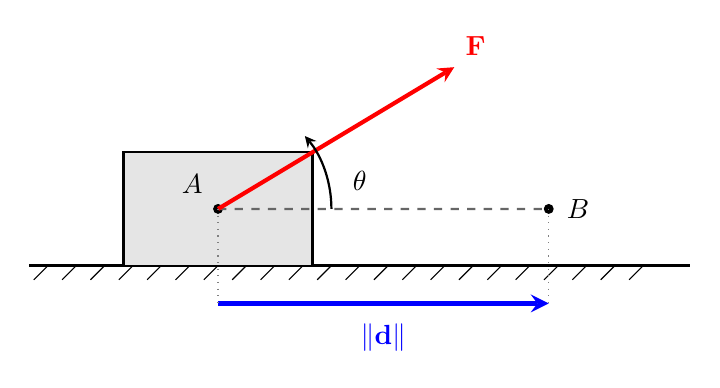
\begin{tikzpicture}[scale=1.2, >=stealth] 

    % 1. Piso / Superficie de apoyo con textura
    \draw[line width=1pt] (-1,0) -- (6,0); 
    \foreach \x in {-0.8,-0.5,...,5.8} {
        \draw (\x,0) -- (\x-0.15,-0.15); 
    }

    % 2. Bloque / Objeto en gris
    \draw[thick, fill=gray!20] (0,0) rectangle (2,1.2); 
    
    % Centro de masa (Punto A: Posición inicial del objeto)
    \coordinate (CM) at (1,0.6); 
    \fill[black] (CM) circle (1.5pt) node[above left=2pt] {$A$}; 

    % 3. Línea auxiliar horizontal (Dirección del movimiento)
    \draw[dashed, black!60, thick] (CM) -- (4.5,0.6); 
    
    % Punto B: Posición final del centro de masa del objeto tras el desplazamiento
    \fill[black] (4.5,0.6) circle (1.5pt) node[right=3pt] {$B$};

    % 4. Vector Fuerza F saliendo de A
    \draw[->, line width=1.5pt, red] (CM) -- (3.5,2.1) node[above right] {$\mathbf{F}$}; 

    % 5. Ángulo theta entre la fuerza y la dirección del movimiento
    \draw[thick, black, ->] (2.2,0.6) arc (0:40:1.2); 
    \node at (2.5,0.9) {$\theta$}; 

    % 6. Vector Desplazamiento posicionado en el suelo (Une las proyecciones de A y B)
    \draw[->, line width=1.8pt, blue] (1, -0.4) -- (4.5, -0.4) node[midway, below=3pt] {$\|\mathbf{d}\|$}; 
    
    % Líneas de proyección tenues que nacen en los puntos A y B hacia el suelo
    \draw[dotted, black!50] (1,0.6) -- (1,-0.4);
    \draw[dotted, black!50] (4.5,0.6) -- (4.5,-0.4);

\end{tikzpicture} 
\end{center} 
    \label{fig:interpretacion fisica}
\end{figure}


\begin{obs}
\textbf{Dependencia del sentido del movimiento.}
Es importante notar que el trabajo es una magnitud que depende intrínsecamente del sentido en el que se recorre el segmento. Si un objeto se desplaza en sentido inverso (desde $B$ hacia $A$), el nuevo vector de desplazamiento es $\mathbf{d}' = A - B = -\mathbf{d}$.  Al calcular el trabajo $W'$ en este recorrido inverso bajo la misma fuerza constante $\mathbf{F}$, obtenemos:
\[ W' = \mathbf{F} \cdot \mathbf{d}' = \mathbf{F} \cdot (-\mathbf{d}) = -(\mathbf{F} \cdot \mathbf{d}) = -W \]
Físicamente, esto significa que si una fuerza realiza un trabajo positivo al acompañar el movimiento en un sentido, realizará exactamente el mismo trabajo pero con signo negativo (se opondrá) si el objeto realiza el camino de regreso. Esta propiedad fundamental se preservará luego al generalizar el concepto mediante la integral de línea.
\end{obs}





\begin{example} 
Un objeto se desplaza desde el punto $A = (0, 0)$ hasta el punto $B = (3, 0)$ a lo largo del segmento que los une, bajo la acción de la fuerza constante $\mathbf{F} = (2, 1)$. Calcular el trabajo realizado por $\mathbf{F}$ sobre el objeto. 

\noindent\textbf{Solución:} Para calcular el trabajo realizado bajo una fuerza constante a lo largo de un segmento rectilíneo, aplicamos la Definición \ref{def:trabajo_fuer_constante}. 
Para ello, en primer lugar, hallamos el vector de desplazamiento $\mathbf{d}$ restando las coordenadas del punto final y el punto inicial:
\[ 
\mathbf{d} = B - A = (3, 0) - (0, 0) = (3, 0). 
\] 
A continuación, siguiendo,  planteamos el producto escalar entre el vector fuerza $\mathbf{F}$ y el vector desplazamiento $\mathbf{d}$:
$$
W = \mathbf{F} \cdot \mathbf{d} = (2, 1) \cdot (3, 0) = 6.
$$
Por lo tanto, el trabajo realizado por la fuerza sobre el objeto es igual a $6$. Como $W > 0$, la fuerza favorece el movimiento; esto concuerda físicamente con el hecho de que el ángulo ($\theta$ entre $\mathbf{F}$ y $\mathbf{d}$ es agudo ($\theta < 90^\circ$). \hfill $\blacksquare$
\end{example}







% =========================================================================
% CONSTRUCCIÓN ANALÍTICA DE LA INTEGRAL DE LÍNEA (TRABAJO MECÁNICO)
% =========================================================================

\subsection*{Construcción Geométrica y Analítica de la Integral de Línea}

Para la siguiente deducci\'on se tendrá en cuenta el caso en el cual $\boldsymbol{\sigma} : [a, b] \to A \subseteq \mathbb{R}^n$ es una trayectoria de clase $\mathcal{C}^1$ y  $\mathbf{F} : A \subseteq \mathbb{R}^n \to \mathbb{R}^n$  es un campo vectorial continuo. Se deja al lector escribir el caso en el cual $\boldsymbol{\sigma}$ es una trayectoria de clase $\mathcal{C}^1$ a trozos. 

\subsubsection*{1. Partición del intervalo paramétrico y discretización}
Sea  $P$   una partición regular del intervalo cerrado $[a, b]$ definida por el conjunto ordenado de puntos $\{t_0, t_1, \dots, t_m\}$ de modo que:
\[
a = t_0 < t_1 < t_2 < \dots < t_i < t_{i+1} < \dots < t_m = b
\]
Esta partición divide al intervalo $ [a, b]$ en $m$ subintervalos de la forma $[t_i, t_{i+1}]$, cada uno con una longitud constante dada por \[\Delta t = t_{i+1} - t_i=\dfrac{b-a}{m} \quad \forall \:  0 \leq  t \leq m.\] Geométricamente, esta partición en  $[a, b]$  induce una subdivisión sobre la trayectoria curva $C =\boldsymbol{\sigma}([a,b])$ en el espacio $\mathbb{R}^n$, delimitada por los puntos de posición discretos $\boldsymbol{\sigma}(t_0), \boldsymbol{\sigma}(t_1), \dots, \boldsymbol{\sigma}(t_m)$.


\subsubsection*{2. Aproximación del desplazamiento y de la fuerza en un subintervalo}
Analicemos el trabajo elemental realizado por el campo sobre el objeto al desplazarse a lo largo del arco de curva que conecta $\boldsymbol{\sigma}(t_i)$ con $\boldsymbol{\sigma}(t_{i+1})$. Si la amplitud del subintervalo $\Delta t_i$ es suficientemente pequeña, dicho arco puede aproximarse mediante el segmento rectilíneo lineal $\mathbf{d}$  que define el desplazamiento neto del tramo, 
\[
\mathbf{d}_i  = \boldsymbol{\sigma}(t_{i+1}) - \boldsymbol{\sigma}(t_i)
\]
Por otra parte, debido a la continuidad asumida para el campo vectorial $\mathbf{F}$, la fuerza que actúa sobre el cuerpo a lo largo de este intervalo local permanece aproximadamente invariable. En consecuencia, es lícito aproximar su valor mediante el campo evaluado en el extremo inferior del subintervalo, esto es, $\mathbf{F}(\boldsymbol{\sigma}(t_i))$. Así, el trabajo elemental $W_i$ efectuado en este tramo se modela a través del producto escalar:
\[
W_i \approx \mathbf{F}(\boldsymbol{\sigma}(t_i)) \cdot \big(  \boldsymbol{\sigma}(t_{i+1}) -  \boldsymbol{\sigma}(t_i) \big)
\]


\subsubsection*{3. Linealización mediante el Teorema del Valor Medio por componentes} 
Dado que la trayectoria $\boldsymbol{\sigma}(t) = \big(\sigma_1(t), \sigma_2(t), \dots, \sigma_n(t)\big)$ es una función vectorial de clase  $\mathcal{C}^1$ , podemos aplicar el Teorema del Valor Medio clásico de una variable a cada una de sus funciones componentes escalares de forma independiente en el subintervalo $[t_i, t_{i+1}]$. Este Teorema garantiza la existencia de puntos intermedios $t^k_i \in (t_i, t_{i+1})$ tales que:
\[
\sigma_k(t_{i+1}) - \sigma_k(t_i) = \sigma_k'(t^k_i)(t_{i+1} - t_i) = \sigma_k'(t^k_i) \Delta t, \quad \text{para cada } k = 1, 2, \dots, n.
\]
Al considerar una partición infinitamente fina, los puntos intermedios convergen al extremo local ($t^k_i \to t_i$). Así, al agrupar nuevamente las componentes en forma de vector, la diferencia de posición se aproxima en términos del vector velocidad $\boldsymbol{\sigma}'(t_i)$ y del paso del parámetro:
\[ 
\boldsymbol{\sigma}(t_{i+1}) - \boldsymbol{\sigma}(t_i) \approx \boldsymbol{\sigma}'(t_i) \Delta t. 
\] 
Al sustituir esta aproximación lineal en la ecuación del trabajo elemental, se obtiene una formulación analítica que depende de manera directa del incremento del parámetro: 
\[ 
W_i \approx \mathbf{F}(\boldsymbol{\sigma}(t_i)) \cdot \boldsymbol{\sigma}'(t_i) \Delta t. 
\] 


\subsubsection*{4. Suma de Riemann y convergencia al límite integral} 
De este modo, obtenemos una primera aproximación al trabajo total $W$ realizado por el campo de fuerzas a lo largo de toda la trayectoria mediante la acumulación de las contribuciones elementales de cada subintervalo, lo cual da lugar a una estructura formal de suma de Riemann: 
\[ 
W \approx \sum_{i=0}^{m-1} W_i = \sum_{i=0}^{m-1} \mathbf{F}(\boldsymbol{\sigma}(t_i)) \cdot \boldsymbol{\sigma}'(t_i) \Delta t. 
\] 

Con base en el análisis anterior, \textbf{definimos formalmente el trabajo realizado por la fuerza variable} como el paso al límite de la suma de Riemann cuando el número de subdivisiones de la partición regular tiende a infinito ($m \to +\infty$): 
\[ 
W = \lim_{m \to +\infty} \sum_{i=0}^{m-1} \mathbf{F}(\boldsymbol{\sigma}(t_i)) \cdot \boldsymbol{\sigma}'(t_i) \Delta t. 
\] 
Dado que el campo vectorial $\mathbf{F}$ es continuo y la trayectoria $\boldsymbol{\sigma}$ es de clase $\mathcal{C}^1$, la función resultante del producto escalar $\mathbf{F}(\boldsymbol{\sigma}(t)) \cdot \boldsymbol{\sigma}'(t)$ es una función escalar continua en el intervalo cerrado $[a,b]$ y, por ende, integrable en el sentido de Riemann. Así, el límite de la suma converge formalmente hacia la integral definida sobre el intervalo paramétrico: 
\[ 
W = \int_a^b \mathbf{F}(\boldsymbol{\sigma}(t)) \cdot \boldsymbol{\sigma}'(t) \, dt. \tag*{$\blacksquare$}
\]
Teniendo en cuenta la Definición \ref{def:Int_tray_a_trozas_vec}  llegamos a la siguiente definic\'on formal

\begin{definition}\label{def:trabajo_trayectoria}\textbf{Trabajo de un campo de fuerzas sobre una trayectoria.} 
Sea $\boldsymbol{\sigma} : [a, b] \to A \subseteq \mathbb{R}^n$ una trayectoria de clase $\mathcal{C}^1$ a trozos y sea $\mathbf{F} : A \subseteq \mathbb{R}^n \to \mathbb{R}^n$ un campo vectorial continuo. Se define el \emph{trabajo realizado por el campo $\mathbf{F}$ sobre la trayectoria $\boldsymbol{\sigma}$}, y se denota por $W$, mediante:
\[ 
W = \int_{\boldsymbol{\sigma}} \mathbf{F} \cdot d\mathbf{s}  
\] 
\end{definition}


\begin{example} \textbf{Dependencia de la orientación.}
 Calcular  el trabajo realizado por el campo \( \mathbf{F}(x, y) = (x, 0) \)  sobre el segmento geométrico del eje $x$  que une los puntos $(0,0)$ y $(1,0)$,   analizando el comportamiento de la integral al recorrerlo en sentidos opuestos.
\end{example}

\noindent\textbf{Solución:} Por un lado, llamemos $W_1$ al trabajo realizado por el campo  $\mathbf{F}$  sobre el segmento si lo recorremos con orientación desde $(0,0)$ hacia $(1,0)$.  Para ello consideremos
\[ \boldsymbol{\sigma}_1(t) = (t, 0), \quad t \in [0, 1] \]

Calculamos su vector derivada:
\[ \boldsymbol{\sigma}_1'(t) = (1, 0) \]

Evaluamos el campo $\mathbf{F}$ sobre la trayectoria sustituyendo $x = t$ e $y = 0$:
\[ \mathbf{F}(\boldsymbol{\sigma}_1(t)) = (t, 0) \]

Calculamos el trabajo $W_1$:
\[ W_1 = \int_{\boldsymbol{\sigma}_1} \mathbf{F} \cdot d\mathbf{s} = \int_{0}^{1} (t, 0) \cdot (1, 0) \, dt = \int_{0}^{1} t \, dt = \left[ \frac{t^2}{2} \right]_{0}^{1} = \frac{1}{2} \]

Por otro lado, llamemos $W_2$ al trabajo realizado por el campo  $\mathbf{F}$  sobre el segmento recorrido de manera inversa, es decir,  con orientación desde $(1,0)$ hacia $(0,0)$.  Para ello consideremos
\[ \boldsymbol{\sigma}_2(t) = (1-t, 0), \quad t \in [0, 1] \]

Calculamos su vector derivada:
\[ \boldsymbol{\sigma}_2'(t) = (-1, 0) \]

Evaluamos el campo $\mathbf{F}$ sobre esta trayectoria sustituyendo $x = 1-t$ e $y = 0$:
\[ \mathbf{F}(\boldsymbol{\sigma}_2(t)) = (1-t, 0) \]

Calculamos el trabajo $W_2$:
\[ W_2 = \int_{\boldsymbol{\sigma}_2} \mathbf{F} \cdot d\mathbf{s} = \int_{0}^{1} (1-t, 0) \cdot (-1, 0) \, dt = \int_{0}^{1} (t-1) \, dt = \left[ \frac{t^2}{2} - t \right]_{0}^{1} = -\frac{1}{2} \]

Como podemos observar, $W_1 = -W_2$.  Esto ilustra de manera explícita que:
\[ \int_{\boldsymbol{\sigma}_1} \mathbf{F} \cdot d\mathbf{s} = -\int_{\boldsymbol{\sigma}_2} \mathbf{F} \cdot d\mathbf{s} \]

Por lo tanto, al invertir el sentido en el que se recorre la trayectoria, el valor absoluto de la integral de línea se mantiene constante, pero \emph{su signo cambia}.







\begin{obs}\label{obs:orientacion_vectorial}
El Ejemplo anterior introduce una de las propiedades más importantes de las integrales de línea de campos vectoriales: \textbf{la dependencia de la orientación}.  A diferencia de los campos escalares, donde el sentido del recorrido no altera el valor de la integral (ver Observación~\ref{obs:param}), en campos vectoriales el signo del trabajo cambia por completo si invertimos el sentido del movimiento. 
\end{obs}



       \subsection{Integral de línea para campos vectoriales}
            

\begin{definition}\label{int_cv} \textbf{Integral de l\'inea para campos vectoriales.}
  Sea $C^{+} \subseteq  \Rn{n}$  una curva simple,  suave a trozos  (definición ~\ref{param}) orientada (definición ~ \ref{orien})  y sea $\boldsymbol{\sigma}:I\subseteq\R\to\mathbb{R}^n $ una parametrizaci\'on regular de $C$ que preserva su orientaci\'on  (definición ~\ref{orien_pre}). Sea $\mathbf{F}:A\subseteq\mathbb{R}^n \to\mathbb{R}^n $ un campo vectorial continuo sobre $C  \subseteq  A.$  Se define la \emph{integral de} $\mathbf{F}$ \emph{sobre la curva} $\boldsymbol{C}^{+}$ como
    \[
        \int_{C^{+}}\mathbf{F}\cdot d\mathbf{s}=\int_{\boldsymbol{\sigma}}\mathbf{F}\cdot d\mathbf{s} 
    \]
\end{definition}

\begin{obs} Bajo las condiciones de \ref{int_cv}, si $\boldsymbol{\beta}$ es una parametrizaci\'on regular de $C$ que no  preserva (o invierte) su orientaci\'on entonces: 
 \[
        \int_{C^{+}}\mathbf{F}\cdot d\mathbf{s}= - \int_{\boldsymbol{\beta}}\mathbf{F}\cdot d\mathbf{s} 
    \]
\end{obs}



       
 \subsection{Proppiedades del Álgebral}
            


  \begin{propertie} \textbf{Algebra de Integral de l\'inea.}\label{alge} Sea $C^{+}$ una curva simple, orientada y suave a trozos, adem\'as,  sean  $\mathbf{F}$ y $\mathbf{G}$ campos vectoriales continuos con dominios tales que incluyen a la curva $C$, entonces: 
\begin{itemize}
\item[1.]  \[
        \int_{C^{+}}(\mathbf{F} + \mathbf{G})  \cdot d\mathbf{s}=  \int_{C^{+}} \mathbf{F} \cdot d\mathbf{s}  +  \int_{C^{+}} \mathbf{G}  \cdot d\mathbf{s} 
    \]

\item[2.]  \[
        \int_{C^{+}} k \mathbf{F}  \cdot d\mathbf{s}= k \int_{C^{+}} \mathbf{F} \cdot d\mathbf{s}   
    \]

\item[3.]  \[
        \int_{C^{+}} k \mathbf{F}  \cdot d\mathbf{s}= - \int_{C^{-}} \mathbf{F} \cdot d\mathbf{s}   
    \]

\item[3.]  Si $C = \cup_{i=1}^{n} C_{i},$ entonces \[
        \int_{C^{+}}  \mathbf{F}  \cdot d\mathbf{s}=  \sum_{i=1}^{n}  \int_{C_{i}^{+}} \mathbf{F} \cdot d\mathbf{s}   
    \]

\end{itemize}
 \end{propertie}



 \begin{tarea} Sea $C$ la curva simple dada por la uni\'on de los segmentos que unen los puntos $(0,0)$,  $(0,3)$ y $(0,2)$. Calcular, indicando la orientaci\'on elegida para $C$  $$ \int_{C}  (y^{2}, 2xy +1)  \cdot d\mathbf{s} $$
 \end{tarea}

 \begin{tarea} Mismo ejercicio con la orientaci\'on para $C$ contraria  a la elegida. 
 \end{tarea}

\begin{tarea}Reescribir  (\ref{alge})  para campos escalares. 
\end{tarea}


\begin{definition}
    Si $C$  es una curva simple cerrada,  se suele notar a la integral como
    \[
        \oint_{C}\mathbf{F}\cdot d\mathbf{s},  
    \]  y se la llama integral de circulaci\'on de $\mathbf{F}$ sobre $C$.
\end{definition}


 \begin{nota}\label{not_int} Sean  $\mathbf{F}=(f_1, f_2)$ y $\mathbf{G}=(g_1, g_2, g_3)$ campos vectoriales, notaremos $$ \int_{C_1}\mathbf{F}\cdot d\mathbf{s} =  \int_{ C_1}f_1\:dx+ f_2 \:dy$$ 
  $$ \int_{C_2}\mathbf{G}\cdot d\mathbf{s} =  \int_{C_2} g_1\:dx+g_2\:dy+g_3\:dz.$$
 \end{nota}
 
 \begin{nota} 
  $\int_{\boldsymbol{\sigma}}\mathbf{F}\cdot d\mathbf{s}=\int_{\boldsymbol{\sigma}}\mathbf{F}\cdot{\mathbf{t}}\:ds$,  donde ${\mathbf{t}}$ es versor tangencial a la curva  $C = Img(\boldsymbol{\sigma}).$
 \end{nota}

         

      
 \section{Campos Conservativos}
 \subsection{Teorema fundamental de las integrales de línea}
 \begin{theorem} \label{thm:t1} 
Sea $A \subseteq \mathbb{R}^n$ un conjunto abierto y arcoconexo (ver la Definición~\ref{def:conjuntoconexo_simp}) y sea $f: A \subseteq \mathbb{R}^n \to \mathbb{R}$ un campo de clase $\mathcal{C}^1(A)$. Además, sea $\boldsymbol{\sigma}: [a,b] \to A \subseteq \mathbb{R}^n$ una trayectoria de clase $\mathcal{C}^{1}$ a trozos. Entonces: 
\[ \int_{\boldsymbol{\sigma}} \nabla f \cdot d\mathbf{s} = f(\boldsymbol{\sigma}(b)) - f(\boldsymbol{\sigma}(a)) \] 
\end{theorem}

\begin{proof}
Demostraremos el caso en el cual $\boldsymbol{\sigma}$ es una trayectoria de clase $\mathcal{C}^{1}$ y se deja al lector probar el caso más general. 

Definamos la función escalar $g(t) = (f \circ \boldsymbol{\sigma})(t)$ con $t \in [a,b]$. Sabemos que $g$ resulta derivable y, por la regla de la cadena, obtenemos: 
\begin{equation*} 
g'(t) = (f \circ \boldsymbol{\sigma})'(t) = \nabla f(\boldsymbol{\sigma}(t)) \cdot \boldsymbol{\sigma}'(t) 
\end{equation*} 

Por el Teorema Fundamental del Cálculo de una variable, sabemos que: 
\begin{equation*} 
\int_{a}^{b} g'(t) \, dt = g(b) - g(a) = f(\boldsymbol{\sigma}(b)) - f(\boldsymbol{\sigma}(a)) 
\end{equation*} 

Por consiguiente:
\begin{align*} 
\int_{\boldsymbol{\sigma}} \nabla f \cdot d\mathbf{s} &= \int_{a}^{b} \nabla f(\boldsymbol{\sigma}(t)) \cdot \boldsymbol{\sigma}'(t) \, dt \\ 
&= \int_{a}^{b} g'(t) \, dt = g(b) - g(a) \\ 
&= f(\boldsymbol{\sigma}(b)) - f(\boldsymbol{\sigma}(a))   \qedhere
\end{align*} 
\end{proof}



\begin{tarea} Para la trayectoria  $\boldsymbol{\sigma}:[0,2]\to A\subseteq\Rn{3}\; : \; \sigma(t) = (t^{3}+1, t^{2}, t^{3}),$  calcular  $$ \int_{\sigma}  (y, x, 0)  \cdot d\mathbf{s} $$
\end{tarea}


\begin{corollary}\label{thm:c1} 
Sean $A \subseteq \mathbb{R}^n$ un conjunto abierto y arcoconexo y $f: A \subseteq \mathbb{R}^n \to \mathbb{R}$ un campo de clase $\mathcal{C}^1(A)$. Si $\boldsymbol{\sigma}_1: [a_1,b_1] \to A$ y $\boldsymbol{\sigma}_2: [a_2,b_2] \to A$ son dos trayectorias de clase $\mathcal{C}^{1}$ a trozos tales que $\boldsymbol{\sigma}_1(a_1) = \boldsymbol{\sigma}_2(a_2) \ \land \ \boldsymbol{\sigma}_1(b_1) = \boldsymbol{\sigma}_2(b_2)$, entonces: 
\[ \int_{\boldsymbol{\sigma}_1} \nabla f \cdot d\mathbf{s} = \int_{\boldsymbol{\sigma}_2} \nabla f \cdot d\mathbf{s} \] 
Es decir, la integral $\int_{\boldsymbol{\sigma}} \nabla f \cdot d\mathbf{s}$ sólo depende de los puntos inicial y final de la trayectoria. 
\end{corollary}

\begin{proof}
Demostraremos el caso en el cual $\boldsymbol{\sigma}_1$ y $\boldsymbol{\sigma}_2$ son trayectorias de clase $\mathcal{C}^{1}$ y se deja al lector probar el caso más general. 

Usando el Teorema~\ref{thm:t1}, se tiene que:
\begin{align*} 
\int_{\boldsymbol{\sigma}_1} \nabla f \cdot d\mathbf{s} &= f(\boldsymbol{\sigma}_1(b_1)) - f(\boldsymbol{\sigma}_1(a_1)) \\ 
\int_{\boldsymbol{\sigma}_2} \nabla f \cdot d\mathbf{s} &= f(\boldsymbol{\sigma}_2(b_2)) - f(\boldsymbol{\sigma}_2(a_2)) 
\end{align*} 

Como por hipótesis $\boldsymbol{\sigma}_1(a_1) = \boldsymbol{\sigma}_2(a_2) \ \land \ \boldsymbol{\sigma}_1(b_1) = \boldsymbol{\sigma}_2(b_2)$, por la buena definición de la función $f$ se cumple que: 
\begin{equation*} 
f(\boldsymbol{\sigma}_1(a_1)) = f(\boldsymbol{\sigma}_2(a_2)) \ \land \ f(\boldsymbol{\sigma}_1(b_1)) = f(\boldsymbol{\sigma}_2(b_2)) 
\end{equation*} 

Luego, restando miembro a miembro obtenemos:
\begin{equation*} 
\int_{\boldsymbol{\sigma}_1} \nabla f \cdot d\mathbf{s} - \int_{\boldsymbol{\sigma}_2} \nabla f \cdot d\mathbf{s} = 0,
\end{equation*} 
lo que demuestra el resultado buscado. 
\end{proof}







 \subsection{Función Potencial}
 \begin{definition}\label{conser} 
Un campo vectorial continuo $\mathbf{F}: A \subseteq \mathbb{R}^n \to \mathbb{R}^n$, con $A$ abierto y arcoconexo, se llama \emph{campo conservativo} si existe una función escalar $f: A \subseteq \mathbb{R}^n \to \mathbb{R}$ de clase $\mathcal{C}^1$ tal que:
\[ \nabla f(\mathbf{x}) = \mathbf{F}(\mathbf{x}), \quad \forall \mathbf{x} \in A \] 
En tal caso, el campo escalar $f$ se llama \emph{función potencial} del campo vectorial $\mathbf{F}$. 
\end{definition}

\begin{propertie}\label{conserv}  Sea $A\subset \Rn{n}$   ($n=2$ o $n=3$)  abierto y arcoconexo y sea  $\mathbf{F}:A  \to \Rn{n}$  de clase $C^{1}(A).$  Si $\mathbf{F}$ es  un campo conservativo entonces $$\nabla \times \mathbf{F}(\mathbf{x}) =0 \:\:\: \forall \mathbf{x} \in A.  $$  
\end{propertie}

\begin{example} Determinar si $\mathbf{F}(x,y,z) = (z\cos xz,\; z,\; y + x\cos xz)$ admite función potencial y, cn caso afirmativo,  hallarla.

Un campo vectorial $\mathbf{F} = (P, Q, R)$
de clase $\mathcal{C}^1$ en un abierto simplemente conexo admite función potencial
si y sólo si $\nabla \times \mathbf{F} = \mathbf{0}$, es decir:
\[
    \frac{\partial R}{\partial y} = \frac{\partial Q}{\partial z}, \qquad
    \frac{\partial P}{\partial z} = \frac{\partial R}{\partial x}, \qquad
    \frac{\partial Q}{\partial x} = \frac{\partial P}{\partial y}.
\]
con $P = z\cos xz$, $Q = z$, $R = y + x\cos xz$.

\[
    \frac{\partial R}{\partial y} = 1, \qquad
    \frac{\partial Q}{\partial z} = 1
\]
 
\[
    \frac{\partial P}{\partial z} = \cos xz + z \cdot (-x\sin xz) = \cos xz - xz\sin xz,
\]

\[
    \frac{\partial R}{\partial x} = \cos xz + x \cdot (-z\sin xz) = \cos xz - xz\sin xz
\]

\[
    \frac{\partial Q}{\partial x} = 0, \qquad
    \frac{\partial P}{\partial y} = 0
\]

Las tres condiciones se satisfacen, luego $\mathbf{F}$ \textbf{admite función potencial}.

\medskip
\textbf{Hallamos $\varphi$ tal que $\nabla\varphi = \mathbf{F}$.} Es decir:
\[
    \frac{\partial \varphi}{\partial x} = z\cos xz, \qquad
    \frac{\partial \varphi}{\partial y} = z, \qquad
    \frac{\partial \varphi}{\partial z} = y + x\cos xz.
\]

\[
    \varphi(x,y,z)
    = \int z\cos xz\, dx
    = z \cdot \frac{\sin xz}{z} + g(y,z)
    = \sin xz + g(y,z).
\]

\[
    \frac{\partial \varphi}{\partial y} = \frac{\partial g}{\partial y} = z
    \implies g(y,z) = yz + h(z).
\]
Luego:
\[
    \varphi(x,y,z) = \sin xz + yz + h(z).
\]

\[
    \frac{\partial \varphi}{\partial z} = x\cos xz + y + h'(z) = y + x\cos xz
    \implies h'(z) = 0 \implies h(z) = C.
\]

\textbf{Función potencial:}
\[
    \boxed{\varphi(x,y,z) = \sin xz + yz + C.}
\]
\end{example}

\begin{example} 
Determinar si el campo vectorial $\mathbf{F}(x,y,z) = (z\cos xz,\; z,\; y + x\cos xz)$ admite función potencial y, en caso afirmativo, hallarla.
\end{example}

\noindent\textbf{Solución:}  El campo vectorial $\mathbf{F} = (P, Q, R)$ está definido en todo $\mathbb{R}^3$ y sus componentes son combinaciones de funciones polinómicas y trigonométricas de clase $\mathcal{C}^1$. 
De acuerdo con la Propiedad~\ref{conserv}, si un campo es conservativo, sus derivadas parciales cruzadas deben ser iguales (lo que equivale a que su rotacional sea nulo).  Por lo tanto, antes de buscar la función potencial, verificamos si se cumplen estas condiciones necesarias:
\[ \frac{\partial R}{\partial y} = \frac{\partial Q}{\partial z}, \qquad \frac{\partial P}{\partial z} = \frac{\partial R}{\partial x}, \qquad \frac{\partial Q}{\partial x} = \frac{\partial P}{\partial y} \]

Identificamos las componentes del campo:
\[ P(x,y,z) = z\cos xz, \qquad Q(x,y,z) = z, \qquad R(x,y,z) = y + x\cos xz \]

Calculamos las derivadas parciales correspondientes:
\begin{align*}
    \frac{\partial R}{\partial y} &= 1, \qquad \frac{\partial Q}{\partial z} = 1 \implies \frac{\partial R}{\partial y} = \frac{\partial Q}{\partial z} \\
    \frac{\partial P}{\partial z} &= \cos xz - xz\sin xz, \qquad \frac{\partial R}{\partial x} = \cos xz - xz\sin xz \implies \frac{\partial P}{\partial z} = \frac{\partial R}{\partial x} \\
    \frac{\partial Q}{\partial x} &= 0, \qquad \frac{\partial P}{\partial y} = 0 \implies \frac{\partial Q}{\partial x} = \frac{\partial P}{\partial y}
\end{align*}

Como las condiciones necesarias se satisfacen, el campo $\mathbf{F}$ es un candidato válido para ser conservativo. Procederemos a intentar construir su función potencial de forma directa en el siguiente paso. Si logramos hallarla con éxito, quedará demostrado que el campo efectivamente admite función potencial.



Buscamos una función escalar $\varphi(x,y,z)$ tal que $\nabla\varphi = \mathbf{F}$. Esto nos plantea el siguiente sistema de ecuaciones diferenciales parciales:
\[ \text{(I)} \ \frac{\partial \varphi}{\partial x} = z\cos xz, \qquad \text{(II)} \ \frac{\partial \varphi}{\partial y} = z, \qquad \text{(III)} \ \frac{\partial \varphi}{\partial z} = y + x\cos xz \]

Comenzamos integrando la ecuación (I) respecto a la variable $x$:
\[ \varphi(x,y,z) = \int z\cos xz\, dx =\sin xz + g(y,z) \]
donde $g(y,z)$ representa la "constante" de integración, la cual puede depender de las variables que se mantuvieron fijas ($y$ y $z$).

Para determinar $g(y,z)$, derivamos la expresión obtenida respecto a $y$ e igualamos con la ecuación (II):
\[ \frac{\partial \varphi}{\partial y} = \frac{\partial g}{\partial y} = z \]
Integrando ahora respecto a $y$, hallamos la forma de la función $g$:
\[ g(y,z) = \int z\, dy = yz + h(z) \]
donde $h(z)$ es una nueva función que depende únicamente de $z$. Sustituyendo esto en nuestra expresión para $\varphi$, tenemos:
\[ \varphi(x,y,z) = \sin xz + yz + h(z) \]

Finalmente, para hallar $h(z)$, derivamos respecto a $z$ e igualamos con la ecuación (III):
\[ \frac{\partial \varphi}{\partial z} = x\cos xz + y + h'(z) = y + x\cos xz \]
Simplificando los términos comunes de ambos lados, obtenemos:
\[ h'(z) = 0 \implies h(z) = C, \quad \text{con } C \in \mathbb{R} \]

\noindent \textbf{Resultado:} La familia de funciones potenciales para el campo vectorial $\mathbf{F}$ es:
\[ \boxed{\varphi(x,y,z) = \sin xz + yz + C} \]




 \subsection{Independencia del camino}
 \begin{corollary}\label{tmh:c2}  Sean $A\subseteq\Rn{n}$ abierto y arcoconexo y $\mathbf{F}:A\subseteq\Rn{n}\to\Rn{n}$  un campo vectorial conservativo entonces para todo par de curvas $C_1$ , $C_2$ simples en $A$, con los mismos puntos extremos y misma orientaci\'on, se tiene que
    \[
    \int_{C_1}\mathbf{F}\cdot d\mathbf{s}=\int_{C_2}\mathbf{F}\cdot d\mathbf{s}. 
    \]
    Dada esta igualdad, se dice que la integral de línea de un campo conservativo tiene \textit{independencia del camino}.

    \textit{Demostración.}   Sean $\boldsymbol{\sigma}_1:[a_1,b_1]\to A$  y $\boldsymbol{\sigma}_2:[a_2,b_2]\to A$  parametrizaciones de  $C_1$ y $C_2$ respectivamente que preservan sus orientaciones y sea  $f$ un funci\'on potencial de $\mathbf{F}$. Por definici\'on  (\ref{int_cv}) se tiene que:
    \begin{align*}
        \int_{C_1}\mathbf{F}\cdot d\mathbf{s}&=\int_{\boldsymbol{\sigma}_1}\grad f\cdot d\mathbf{s}\\
        \int_{C_2}\mathbf{F}\cdot d\mathbf{s}&=\int_{\boldsymbol{\sigma}_2}\grad f\cdot d\mathbf{s}
    \end{align*}
    Además, como $C_1$ y $C_2$ tienen lo mismos puntos extremos, entonces $\boldsymbol{\sigma}_1(a_1)=\boldsymbol{\sigma}_2(a_2)\;\land\;\boldsymbol{\sigma}_1(b_1)=\boldsymbol{\sigma}_2(b_2)$.
    Por lo tanto,  por el Corolario \ref{tmh:c1}:
    $$  \int_{\boldsymbol{\sigma}_1}\grad f\cdot d\mathbf{s}=\int_{\boldsymbol{\sigma}_2}\grad f\cdot d\mathbf{s} $$
     lo que demuestra que:   $$ \int_{C_1}\mathbf{F}\cdot d\mathbf{s}=\int_{C_2}\mathbf{F}\cdot d\mathbf{s}$$
   
\end{corollary}




\begin{corollary}\label{tmh:c2} 
Sean $A \subseteq \mathbb{R}^n$ abierto y arcoconexo y $\mathbf{F}: A \subseteq \mathbb{R}^n \to \mathbb{R}^n$ un campo vectorial conservativo. Entonces, para todo par de curvas $C_1$ y $C_2$ simples en $A$, con los mismos puntos extremos y misma orientación, se tiene que: 
\[ \int_{C_1} \mathbf{F} \cdot d\mathbf{s} = \int_{C_2} \mathbf{F} \cdot d\mathbf{s} \] 
Dada esta igualdad, se dice que la integral de línea de un campo conservativo tiene \emph{independencia del camino}. 
\end{corollary}

\begin{proof}
Sean $\boldsymbol{\sigma}_1: [a_1,b_1] \to A$ y $\boldsymbol{\sigma}_2: [a_2,b_2] \to A$ parametrizaciones de $C_1$ y $C_2$ respectivamente que preservan sus orientaciones, y sea $f$ una función potencial de $\mathbf{F}$. 

Por la Definición~\ref{int_cv} y sabiendo que $\mathbf{F} = \nabla f$, se tiene que: 
\begin{align*} 
\int_{C_1} \mathbf{F} \cdot d\mathbf{s} &= \int_{\boldsymbol{\sigma}_1} \nabla f \cdot d\mathbf{s} \\ 
\int_{C_2} \mathbf{F} \cdot d\mathbf{s} &= \int_{\boldsymbol{\sigma}_2} \nabla f \cdot d\mathbf{s} 
\end{align*} 

Además, dado que $C_1$ y $C_2$ comparten los mismos puntos extremos y el mismo sentido de recorrido, sus parametrizaciones satisfacen que $\boldsymbol{\sigma}_1(a_1) = \boldsymbol{\sigma}_2(a_2) \ \land \ \boldsymbol{\sigma}_1(b_1) = \boldsymbol{\sigma}_2(b_2)$. 

Por lo tanto, aplicando el Corolario~\ref{thm:c1}, obtenemos: 
\[ \int_{\boldsymbol{\sigma}_1} \nabla f \cdot d\mathbf{s} = \int_{\boldsymbol{\sigma}_2} \nabla f \cdot d\mathbf{s} \] 
Lo que demuestra finalmente:
\[ \int_{C_1} \mathbf{F} \cdot d\mathbf{s} = \int_{C_2} \mathbf{F} \cdot d\mathbf{s} \qedhere \] 
\end{proof}


\begin{corollary}\label{tmh:c3} 
Sean $A \subseteq \mathbb{R}^n$ abierto y arcoconexo y $\mathbf{F}: A \subseteq \mathbb{R}^n \to \mathbb{R}^n$ un campo vectorial conservativo. Entonces, para toda curva $C$ simple cerrada contenida en $A$, se cumple que: 
\[ \oint_C \mathbf{F} \cdot d\mathbf{s} = 0 \] 
\end{corollary}

\begin{proof}
Sea $f$ una función potencial de $\mathbf{F}$ y sea $\boldsymbol{\sigma}: [a,b] \to A$ una parametrización de $C$ que preserva su orientación. Entonces, por la Definición~\ref{int_cv} y sabiendo que $\mathbf{F} = \nabla f$, tenemos: 
\begin{equation*} 
\oint_C \mathbf{F} \cdot d\mathbf{s} = \int_{\boldsymbol{\sigma}} \nabla f \cdot d\mathbf{s} 
\end{equation*} 

Por el Teorema~\ref{thm:t1}, sabemos que: 
\begin{equation*} 
\int_{\boldsymbol{\sigma}} \nabla f \cdot d\mathbf{s} = f(\boldsymbol{\sigma}(b)) - f(\boldsymbol{\sigma}(a)) 
\end{equation*} 

Además, dado que la curva $C$ es cerrada, su punto final coincide con su punto inicial, lo que significa que $\boldsymbol{\sigma}(b) = \boldsymbol{\sigma}(a)$. Por la buena definición de la función $f$, se cumple que $f(\boldsymbol{\sigma}(b)) = f(\boldsymbol{\sigma}(a))$. 

Sustituyendo esta igualdad en la ecuación anterior, obtenemos:
\[ f(\boldsymbol{\sigma}(b)) - f(\boldsymbol{\sigma}(a)) = 0 \]
Lo que demuestra finalmente que: 
\[ \oint_C \mathbf{F} \cdot d\mathbf{s} = 0 \qedhere \] 
\end{proof}









 \subsection{Teorema: Independencia y Potencial}
 \begin{theorem}\label{tmh:t2}
   Sea  $\mathbf{F}:A\subseteq\Rn{n} \to \Rn{n}$ continuo con  $A$ abierto y conexo. Si  $\int_C \mathbf{F}\cdot d\mathbf{s}$ es independiente del camino en $A$  entonces el campo
    $$f:A\subseteq\Rn{n}\to\R\: | \:f(\mathbf{x})=\int_{\mathbf{x}_0}^{\mathbf{x}}\mathbf{F}\cdot d\mathbf{s},  \mbox{ con }  \mathbf{x}_0\in A, $$
    cumple que: 
    \begin{enumerate}
        \item $f$ es $\mathcal{C}^1$.
        \item $\grad f(\mathbf{x})=\mathbf{F}(\mathbf{x})\quad\forall\:\mathbf{x}\in A.$
    \end{enumerate}
\end{theorem}
 \subsection{Equivalencias de Campos Conservativos}
 \begin{theorem}\label{thm:equivalencias_conservativos}
Sea $\mathbf{F}: A \subseteq \mathbb{R}^n \to \mathbb{R}^n$ un campo vectorial continuo, con $A$ un conjunto abierto y arcoconexo. Las siguientes afirmaciones son equivalentes:
\begin{enumerate}
    \item $\mathbf{F}$ es un campo vectorial conservativo en $A$.
    \item La integral de línea de $\mathbf{F}$ es independiente del camino en $A$.
    \item $\oint_C \mathbf{F} \cdot d\mathbf{s} = 0$ para toda curva simple, cerrada y orientada $C$ contenida en $A$.
\end{enumerate}
\end{theorem}

    \textit{Demostración.} 
    \begin{itemize}
\item[] ($1 \Rightarrow 2.)$  Ver \ref{tmh:c2}
\item[] ($2 \Rightarrow 3.)$ Sea $C^{+}$ una curva simple, cerrada y orientada en $A$. Pensemos que a dicha curva la podemos ver como la uni\'on de  dos curvas   simples orientadas en $A$,  $C_1$ , $C_2$,  cuyas orientaciones son heredadas de $C$,   con los mismos puntos extremos,  tal como muestra la figura. 

\begin{figure}[htbp]
    \centering
    % Llamamos al archivo con el código TikZ extraído
    \begin{figure}[H]
        \begin{center}
            \begin{tikzpicture}[scale=2, >=stealth]

                % Puntos A y B
                \coordinate (A) at (0,0);
                \coordinate (B) at (3,0);

                % Primer camino: curva hacia arriba (gamma_1)
                \draw[thick, blue, ->, decoration={markings, mark=at position 0.5 with {\arrow{>}}},
                    postaction={decorate}] 
                    (A) .. controls (1,1.5) and (2,1.5) .. (B) node[midway, above] {$C_1$};

                % Segundo camino: curva hacia abajo (gamma_2)
                \draw[thick, red, ->, decoration={markings, mark=at position 0.5 with {\arrow{>}}},
                    postaction={decorate}] 
                    (B) .. controls (1,-1.5) and (2,-1.5) .. (A) node[midway, below] {$C_2$};

                % Nombres de los puntos
                \filldraw (A) circle(0.03) node[below left] {$A$};
                \filldraw (B) circle(0.03) node[below right] {$B$};

            \end{tikzpicture}
            \caption{Curvas $C_1$ y $C_2$.}
        \end{center}
    \end{figure} 
    \label{fig:campo conservativo}
\end{figure}

   Es decir,  $C^{+}=C_1^{+} \cup C_2^{-}$.  Así:
    \begin{align*}
        \oint_{C^{+}} \mathbf{F}\cdot d\mathbf{s}&=\int_{C_1^{+}}\mathbf{F}\cdot d\mathbf{s}+\int_{C_2^{-}}\mathbf{F}\cdot d\mathbf{s}\\
        &=\int_{C_1^{+}}\mathbf{F}\cdot d\mathbf{s}-\int_{C_2^{+}}\mathbf{F}\cdot d\mathbf{s} =0 \ 
          \end{align*}
   \item[] ($3 \Rightarrow 1$.) Queda a cargo del lector.   
\end{itemize}


\begin{tarea}  Probar que el campo $\mathbf{F}$  tiene rotor nulo en todo $\mathbb{R}^{2}$ y, sin embargo, no es un campo conservativo. ( No vale la vuelta de de la Propiedad (\ref{conserv})).   $$F(x,y) = (\dfrac{y}{x^{2}+y^{2}}, \dfrac{-x}{x^{2}+y^{2}}) $$
\end{tarea}






  
  \chapter{Integrales dobles y triples de  campos escalares.}
      \section{Integrales Dobles} 
        \subsection{Integrales Dobles sobre Rectángulos}
        \begin{definition}  \textbf{Rect\'angulo.} Al conjunto \( B  \subseteq  \mathbb{R}^2 \) dado por
	\[
	B = [a, b] \times [c, d] = \{(x, y) \in \mathbb{R}^2 \mid a \leq x \leq b, \; c \leq y \leq d\}
	\]
	se lo llama rect\'angulo.   
\end{definition}	

\begin{definition} \textbf{Partici\'on regular.} 	Sea \( B  \subseteq  \mathbb{R}^2 \) un rect\'angulo.  Una partición regular de $B$ es un conjunto de pequeños rectángulos disjuntos (salvo tal vez por sus bordes)  de igual \'area que  generan una subdivisi\'on de $B$.  Es decir, si $B = [a, b] \times [c, d]$,  esto se logra dividiendo:
	
	\begin{itemize}
		\item el intervalo \( [a, b] \) en \( n \) subintervalos \( [x_i, x_{i+1}] \) con $0 \leq  i \leq n-1$, cada uno de ancho \( \Delta x \),
		\item el intervalo \( [c, d] \) en \( m \) subintervalos \( [y_j, y_{j+1}] \) con $0 \leq  j \leq m-1$, cada uno de ancho \( \Delta y \).
	\end{itemize}
y tomando los subrect\'angulos $B_{ij}$ tales que
	\[
	B_{ij} = [x_i, x_{i+1}] \times [y_j, y_{j+1}], 
	\]  El \'area de $ B_{ij}$ la notaremos por $\Delta B_{ij}$ 
\end{definition}


\begin{definition}
Dada una funci\'on $f:B\to\R$, donde $B$ es un rect\'angulo en $\Rn{2}$, se define la suma de Reimann de $f$ sobre $B$ a 
\[
    S_{n,m}=\sum_{i=0}^{n-1}\sum_{j=0}^{m-1} f(c_{ij})\Delta B_{ij},
\]  
donde $\{ B_{ij}\}_{( 1 \leq i \leq n, 1 \leq j \leq m )}$ es una partici\'on regular de $B$ y  $c_{ij}\in B_{ij} \: \forall \: 1 \leq i \leq n, 1 \leq j \leq m$. 
\end{definition}

\begin{definition} 
    Sea $f:B=[a,b]\times[c,d]\to\R$ una funci\'on. Diremos que $f$ es integrable sobre $B$ si  el l\'imite $\lim_{(n,m)\to (\infty,\infty)}S_{n,m}$  existe y es finito, en tal caso el valor de dicho  l\'imite  se llama \textbf{integral doble} de $f$ sobre $B$ y se nota 
    \[
          \iint_B f\:dA  \mbox{ o } \iint_B f(x,y)\:dxdy.
    \]
\end{definition}

\begin{obs}
Para que exista el límite,  es suficiente que $f$ sea acotada sobre el rectángulo $B$, y el conjunto de puntos de (posibles) discontínuidades  sea la unión finita de gráficas
de funciones continuas. Es decir, $f$ contínua, excepto, tal vez, sobre curvas.
\end{obs}


          \subsection{Integrales sobles sobre conjuntos generales}
         
Para extender esta noci\'on de integral a  conjuntos acotados m\'as generales que no sean  rect\'angulos, definimos lo siguiente. 

\begin{definition}\label{def:int_D}
Sean $D  \subseteq  \mathbb{R}^{2}$,  $f:D \to\R$ contínua y $R=[a,b]\times[c,d]$ tal que $D  \subseteq  R$.  Se define la funci\'on $f^*$ tal que 
\[
    f^*(x,y)=
    \begin{dcases*}
        f(x,y) & si $(x,y)\in D$ \\[.2cm]
        0        & si $(x,y)\in R \setminus D.$
    \end{dcases*}
\]

Dada su definici\'on, $f^*$ no tiene porque ser continua sobre todo $R$ pero de tener discontinuidades  las mismas estar\'an sobre  $\partial D$. Luego, si $\partial D$ est\'a formada por una curva continua entonces $f^*$ es integrable y  se define la integral de $f$ sobre $D$ por
\[
    \iint_D f\:dA=\iint_B f^*\:dA.  
\]
\end{definition}
La explicación se puede observar mejor en la siguiente figura:


 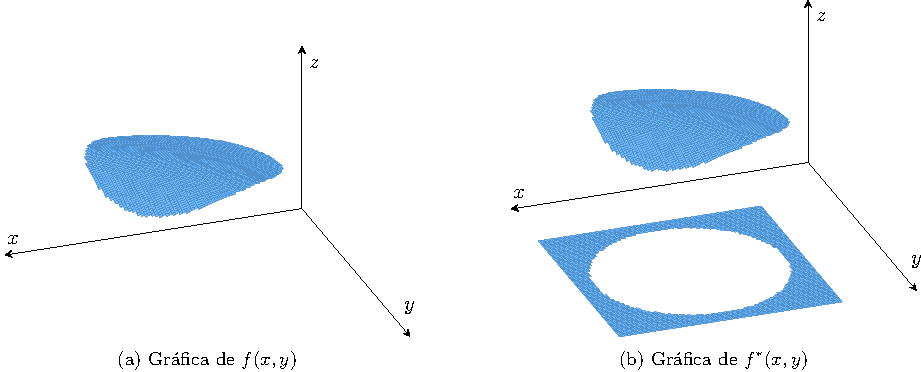
\includegraphics{standalone_fig_integral.pdf}

%\begin{figure}[H]
 %   \centering
 % === Subfigura (a) ===
 %   \begin{subfigure}[b]{0.45\textwidth}
 %   \centering
  %  \begin{tikzpicture}
  %  \begin{axis}[
    %    view={160}{40},
     %   xmin=0, xmax=2,
   %     ymin=0, ymax=2,
    %    zmin=0, zmax=3,
     %   axis lines=center,
     %   ticks=none,
     %   xlabel={$x$}, ylabel={$y$}, zlabel={$z$},
     %   domain=0:2, y domain=0:2,
     %   samples=30, z buffer=sort
  %  ]
        % Región R (rectángulo base)
     %   \addplot3[
    % surf,
  %  shader=faceted,
  %  draw=black, % dibuja las líneas de la malla
   % fill=gray, fill opacity=0.2,
  %  domain=0.5:2, y domain=0.5:2,
  %  samples=20
%] {0};

    %    % Superficie sobre región R (solo en R)
     %   \addplot3[
      %      surf, opacity=0.7, colormap={mycolor}{rgb255=(100,180,255) rgb255=(100,180,255)},
        %    domain=0.5:2, y domain=0.5:2,
      %  ] {sin(x*y*50)+2};
   % \end{axis}
   % \end{tikzpicture}
    % \caption{Gráfica de \( f(x,y) \) sobre  \( R \)}
    % \end{subfigure}
    % \hfill
    % === Subfigura (b) ===
    % \begin{subfigure}[b]{0.45\textwidth}
   % \centering
   % \begin{tikzpicture}
   % \begin{axis}[
     %   view={160}{40},
     %   xmin=0, xmax=2,
     %   ymin=0, ymax=2,
     %   zmin=0, zmax=3,
     %   axis lines=center,
      %  ticks=none,
      %  xlabel={$x$}, ylabel={$y$}, zlabel={$z$},
       %  domain=0:2, y domain=0:2,
      %  samples=60, z buffer=sort
   % ]

     %   % Superficie f(x,y) sobre toda R, con 0 fuera de D
     %   \addplot3[
       %     surf, opacity=0.8,
      %      domain=0.5:1.5, y domain=0.5:1.5,
       %     colormap={mycolor}{rgb255=(100,180,255) rgb255=(100,180,255)},
        %     restrict z to domain=2.1:10, % recorta para evitar planicies
   % unbounded coords=jump,
    %    ]
      %  { ( (x-1)^2 + (y-1)^2 < 0.2 ) * sin(x*y*50)+2 };

         % Región R en gris claro
     % \addplot3[
   % surf,
  %  shader=faceted,
   % draw=black, % dibuja las líneas de la malla
   % fill=gray, fill opacity=0.2,
   % domain=0.5:2, y domain=0.5:2,
  %  samples=20
%] {0};
        
       % \addplot3[
        %    surf, opacity=0.8,
         %   domain=0.5:2, y domain=0.5:2,
        %    colormap={mycolor}{rgb255=(100,180,255) rgb255=(100,180,255)},
      %       restrict z to domain=-0.1:0.1, % recorta para evitar planicies
  %  unbounded coords=jump,
      %  ]
      %  { ( (x-1)^2 + (y-1)^2 < 0.2 ) + 0 };

  %  \end{axis}
   % \end{tikzpicture}
  %  \caption{Gráfica de \( f^*(x,y) \) sobre \( R \)}
  %  \end{subfigure}
%\end{figure}

























\begin{obs} 
La  \autoref{def:int_D}  es independiente  de la selecci\'on de $B$.
\end{obs}

\begin{propertie}
    Sean $f,\;g$ dos funciones integrables en una regi\'on $D\subset\Rn{2}$, entonces:
    \begin{enumerate}
        \item[i.] $\alpha f+\beta g$ es integrable en $D$, $\forall\;\alpha,\;\beta\in\R$ y, adem\'as,
        \[
            \iint_D \left(\alpha f+\beta g\right)dA=\alpha\iint_D f\:dA+\beta\iint_D g\:dA.
        \]
        \item[ii.] El producto $fg$ es integrable en $D$.
        \item[iii.] Si $g(x,y) \neq 0\;\forall(x,y)\in D$ entonces el cociente $f/g$ es integrable en $D$.
        \item[iv.] Si $f(x,y)\geq 0 \;\forall(x,y)\in D$ entonces  $\iint_D f\:dA\geq0$.
        \item[v.]Si $f(x,y)\leq g(x,y)  \;\forall(x,y)\in D$ entonces $\iint_D f\:dA\leq\iint_D g\:dA.$
        \item[vi.]Si $|f|$ es integrable en $D$ entonces 
        \[
            \left|\iint_D f\:dA\right|\leq\iint_D|f|\:dA.  
        \]    
        \item[vii.] Si $D=D_1\cup D_2$ donde $\;D_1\cap D_2$ es un conjunto de medida nula  entonces   $f$ es integrable sobre $D_1$ y sobre $D_2$ y, adem\'as,  
        \[
            \iint_D f\:dA=\iint_{D_1} f\:dA+\iint_{D_2}f\:dA.    
        \]
    \end{enumerate}
\end{propertie}

          \subsection{Integrales dobles sobre conjuntos elementales}
          \begin{definition}\label{conj_elem}  Un conjunto  $D\subseteq\Rn{2}$ se llama elemental si  puede ser descripto de alguna de las siguientes maneras. 
   
    \begin{enumerate}
    \item[i.] Si  existen funciones $\phi_1,\;\phi_2:[a,b]\to\R$  continuas  tales que $ \phi_1(x) < \phi_2(x) \: \forall x \in (a,b) $  y:
    \begin{equation}\label{def:tipo1}
     D = \{ (x,y) \in \mathbb{R}^{2}: \:   x\in[a,b] \: \land \: \phi_1(x)\leq y\leq\phi_2(x) ;\forall\;x\in[a,b] \}  
     \end{equation}   En tal caso  el conjunto $D$ se llama  \textit{elemental de tipo 1.} 
   
    \item[ii.]Si existen funciones $\psi_1,\;\psi_2:[c,d]\to\R$  continuas tales que $ \psi_1(y) < \psi_2(y) \: \forall y \in (c,d)$ y 
    \begin{equation}\label{def:tipo2}
     D = \{ (x,y) \in \mathbb{R}^{2}:   y\in[c,d] \: \land \:  \psi_1(y)\leq x\leq\psi_2(y) ;\forall\;y\in[c,d] \}  
     \end{equation}
     En tal caso el conjunto $D$  se llama  \textit{elemental de tipo 2.} 
    
    \item[iii.] $D$ se llama conjunto elemental de \textit{tipo 3} si es \textit{tipo 1} y \textit{tipo 2} a la vez.
    
    \input{figs/conj-elementales.tex}
    
    \end{enumerate}
\end{definition}

\begin{example}
    Para poder clasificar a una regi\'on como tipo 3 es necesario poder encontrar simult\'aneamente funciones $\phi_1$, $\phi_2$, $\psi_1$ y $\psi_2$ tales que
    \[
    \begin{dcases}
        \phi_1(x)\leq y\leq\phi_2(x) & x\in[a,b]\\[.2cm]
        \psi_1(y)\leq x\leq\psi_2(y) & y\in[c,d].
    \end{dcases}
    \]
    Un ejemplo simple de tal regi\'on es un c\'irculo, donde la ecuaci\'on de esta regi\'on es $$D=\{(x,y)\in\Rn{2}:(x-x_0)^2+(y-y_0)^2\leq r\}.$$  

    \input{figs/ex_tipo3.tex}

    Para describir esta regi\'on como Tipo $1$  debemos despejar $y$ en funci\'on de $x$, esto es,
 
 \textcolor{red}{Agregar los dos dibujos marcando claramete cada una de las situaciones }

   \[
        \phi_1(x)=-\sqrt{r-(x-x_0)^2}+y_0,\quad x\in[x_0-r,x_0+r],
    \]
    y
    \[
        \phi_2(x)=\sqrt{r-(x-x_0)^2}+y_0,\quad x\in[x_0-r,x_0+r].
    \]

    Puede observarse que $D$ es una regi\'on de tipo 1:

    \begin{center}
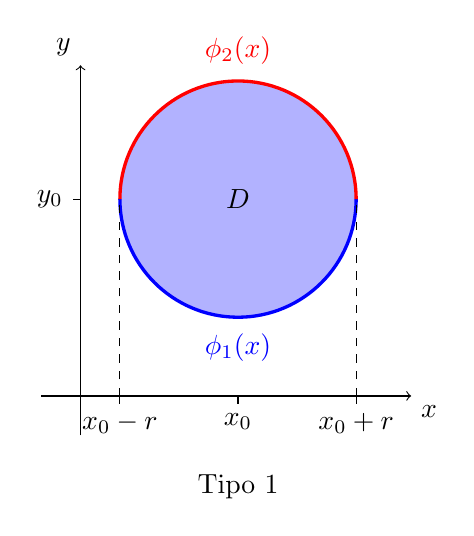
\begin{tikzpicture}
    % parámetros
    \def\cx{2}    % x_0
    \def\cy{2.5}    % y_0
    \def\rr{1.5}  % r

    %—————— Región Tipo 1 (despeje de y en función de x) ——————
    \begin{scope}
        % ejes
        \draw[->] (-0.5,0) -- (4.2,0) node[below right] {$x$};
        \draw[->] (0,-0.5) -- (0,4.2) node[above left]  {$y$};

        % relleno del círculo
        \fill[blue!30] (\cx,\cy) circle [radius=\rr];

        % semicircunferencia inferior: phi_1(x) = -sqrt(r-(x-x0)^2)+y0
        \draw[blue, very thick] (\cx-\rr,\cy) arc[start angle=180, end angle=360, radius=\rr]
            node[midway, below, yshift=-2pt] {\color{blue}$\phi_1(x)$};
        % semicircunferencia superior: phi_2(x) = +sqrt(r-(x-x0)^2)+y0
        \draw[red, very thick] (\cx-\rr,\cy) arc[start angle=180, end angle=0, radius=\rr]
            node[midway, above, yshift=2pt] {\color{red}$\phi_2(x)$};

        % líneas punteadas verticales en x_0 - r y x_0 + r
        \draw[dashed] (\cx-\rr,0) -- (\cx-\rr,\cy);
        \draw[dashed] (\cx+\rr,0) -- (\cx+\rr,\cy);

        % ticks y etiquetas en el eje x
        \draw (\cx-\rr,0) -- ++(0,-0.1) node[below] {$x_0-r$};
        \draw (\cx,0)     -- ++(0,-0.1) node[below] {$x_0$};
        \draw (\cx+\rr,0) -- ++(0,-0.1) node[below] {$x_0+r$};
        % tick y etiqueta en y_0
        \draw (0,\cy) -- ++(-0.1,0) node[left] {$y_0$};

        % etiqueta D
        \node at (\cx,\cy) {$D$};

        % título
        \node[below, yshift=-22pt] at (\cx,-0.1) {Tipo 1};
    \end{scope}
    \end{tikzpicture}
    \end{center}


    A su vez,  para describir esta regi\'on como Tipo $2$  debemos despejar $x$ en funci\'on de $y$, esto es, 
    \[
        \psi_1(y)=-\sqrt{r-(y-y_0)^2}+x_0,\quad y\in[y_0-r,y_0+r],
    \]
    y
    \[
        \psi_2(y)=\sqrt{r-(y-y_0)^2}+x_0,\quad y\in[y_0-r,y_0+r].
    \]
    Puede observarse que $D$ es una regi\'on de tipo 2:
    \begin{center}
        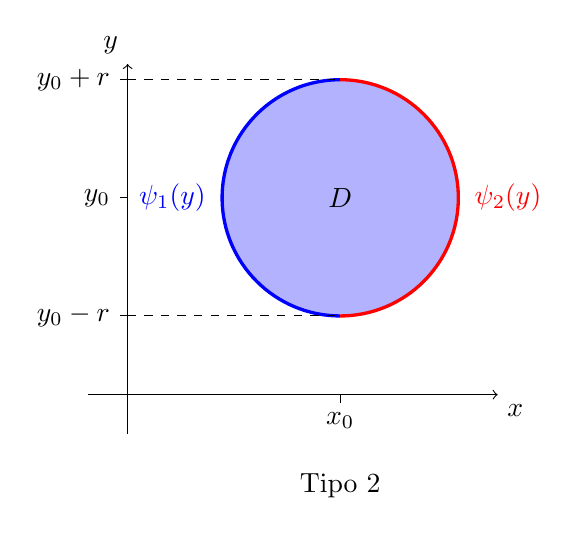
\begin{tikzpicture}
     \begin{scope}[xshift=7cm]
        \def\cxx{2.7}
        \def\cx{2}    % x_0
        \def\cy{2.5}    % y_0
        \def\rr{1.5}  % r

        % ejes
        \draw[->] (-0.5,0) -- (4.7,0) node[below right] {$x$};
        \draw[->] (0,-0.5) -- (0,4.2) node[above left]  {$y$};

        % relleno del círculo
        \fill[blue!30] (\cxx,\cy) circle [radius=\rr];

        % semicircunferencia izquierda: psi_1(y) = -sqrt(r-(y-y0)^2)+x0
        \draw[blue, very thick] (\cxx,\cy-\rr) arc[start angle=270, end angle=90, radius=\rr]
            node[midway, left, xshift=-2pt] {\color{blue}$\psi_1(y)$};
        % semicircunferencia derecha: psi_2(y) = +sqrt(r-(y-y0)^2)+x0
        \draw[red, very thick] (\cxx,\cy-\rr) arc[start angle=-90, end angle=90, radius=\rr]
            node[midway, right, xshift=2pt] {\color{red}$\psi_2(y)$};

        % líneas punteadas horizontales en y_0 - r y y_0 + r
        \draw[dashed] (0,\cy-\rr) -- (\cxx,\cy-\rr);
        \draw[dashed] (0,\cy+\rr) -- (\cxx,\cy+\rr);

        % ticks y etiquetas en el eje y
        \draw (0,\cy-\rr) -- ++(-0.1,0) node[left] {$y_0-r$};
        \draw (0,\cy)     -- ++(-0.1,0) node[left] {$y_0$};
        \draw (0,\cy+\rr) -- ++(-0.1,0) node[left] {$y_0+r$};
        % tick y etiqueta en x_0
        \draw (\cxx,0) -- ++(0,-0.1) node[below] {$x_0$};

        % etiqueta D
        \node at (\cxx,\cy) {$D$};

        % título
        \node[below, yshift=-22pt] at (\cxx,-0.1) {Tipo 2};
    \end{scope}
\end{tikzpicture}
\end{center}
    Por tanto, $D$ es una regi\'on de tipo 3.
\end{example}


         \subsection{Teorema de Fubbini}
        
\begin{theorem}  \label{col:fubini} \textbf{Teorema de Fubini} en $\mathbb{R}^{2}.$  Sea $f:D\to\R$ continua sobre  $D\subseteq\Rn{2}$  un conjunto elemental   (\ref{conj_elem}) 
   
\begin{enumerate} 
        \item  Si $D$ es de Tipo 1 (\ref{def:tipo1})   entonces la integral doble de $f$ sobre $D$ se puede calcular
        \[
            \iint_D f=\int_a^b\left(\int_{\phi_1(x)}^{\phi_2(x)}f(x,y)\:dy\right)dx.  
        \]
       
        \item   Si $D$ es de Tipo 2 (\ref{def:tipo2})  entonces la integral doble de $f$ sobre $D$ se puede calcular
        \[
            \iint_D f=\int_c^d\left(\int_{\psi_1(y)}^{\psi_2(y)}f(x,y)\:dx\right)dy.  
        \]
       
        \item Si $D$ es de Tipo 3   entonces la integral doble de $f$ sobre $D$ se puede calcular  
         \[
            \iint_D f=\int_a^b\left(\int_{\phi_1(x)}^{\phi_2(x)}f(x,y)\:dy\right)dx=\int_c^d\left(\int_{\psi_1(y)}^{\psi_2(y)}f(x,y)\:dx\right)dy. 
        \]
    \end{enumerate}
\end{theorem}


\begin{obs} La \'unica manera de demostrar que un conjunto es elemental es dando su descripci\'on  impl\'icita.
\end{obs}


\begin{example}
     Sean $f(x,y)=x^2y$ y  $D$ es la regi\'on del plano encerrada por $y=x^3$, $y=x^2$  con $x\in[0,1]$,  calcular,  $$\iint_D f \:dA.$$  
\end{example}

\begin{figure}[htbp]
    \centering
    % Llamamos al archivo con el código TikZ extraído
    \begin{center}
    \begin{tikzpicture}
        \begin{axis}[
            axis lines = middle,
            xmin = 0, xmax = 1.5,
            ymin = 0, ymax = 1.5,
            xlabel = {$x$},
            ylabel = {$y$},
            domain = 0:1.25,
            samples = 100,
            xtick={0.5,1},
            ytick={0.5,1},
            clip=false,
            ]
        
            % Define the curves
            \addplot[name path=A, blue, thick, domain=0:1.22] {x^2} node[pos=0.75, right] {$y=x^2$};
            \addplot[name path=B, red, thick, domain=0:1.15] {x^3} node[pos=0.3, below right] {$y=x^3$};
        
            % Fill the area between the curves
            \addplot[orange!50, fill opacity=0.5] fill between[of=A and B, soft clip={domain=0:1}];
        
            % Label the enclosed area as D
            \node at (axis cs:0.6,0.29) {$D$};
        
        \end{axis}
    \end{tikzpicture}
    \end{center}
 
    \label{fig:ejemplo 812}
\end{figure}

\textbf{Soluci\'on:} $D$ puede ser descripto de la siguiente manera
    \[
        D=\{(x,y)\in\Rn{2}:0\leq x\leq1;\;x^3\leq y\leq x^2\},  
    \]
 por lo tanto $D$ es elemetal de Tipo 1 y  por el \autoref{col:fubini}
    \begin{gather*}
        \iint_D x^2y\:dA=\int_0^1\left(\int_{x^3}^{x^2}\:dy\right)dx=\int_0^1\left(x^2\frac{1}{2}y^2\Big\lvert_{x^3}^{x^2}\right)dx\\
        =\int_0^1\frac{1}{2}x^2\left((x^2)^2-(x^3)^2\right)=\int_0^1\frac{1}{2}x^6-\frac{1}{2}x^8\;dx\\=\frac{1}{14}x^7-\frac{1}{18}x^9\Big\lvert_0^1=\frac{1}{14}-\frac{1}{18}=\frac{1}{63}.
    \end{gather*}


\begin{tarea}Calcular  $$ \int_{0}^{1}\int_{y}^{1} e^{x^{2}} \:\: dx\:dy $$
\end{tarea}



\begin{definition}  
    \label{def:area}
    Sea $D\subset\Rn{2}$,  se define el \'area de $D$,  y se denota $\text{A}(D)$,  a  
    \[
        \text{A}(D)=\iint_D1\:dA.
    \]
\end{definition}

          \subsection{Teorema de Valor Medio Integral}
           
\begin{theorem}
    \textbf{Teorema del valor medio para integrales dobles.}   Sea $f:D\subseteq\Rn{2}\to\R$ continual.  Entonces existe $(x_0,y_0)$ en $D$ tal que
    \[
        \int_D f(x,y)\:dA=f(x_0,y_0)\text{A}(D).
    \]
\end{theorem}

\begin{definition}
    Sea $\mathbf{F}:A\subseteq\Rn{n}\to\Rn{n}$ un campo $\mathcal{C}^1(A)$ y sea $\boldsymbol{D}_\mathbf{F}$ (\autoref{def:mat_dif}) su matriz diferencial.  Se define el \emph{jacobiano}, o \emph{determinante jacobiano}, y se lo nota $J_\mathbf{F}$ a 
    \[
        J_\mathbf{F}=\text{det}(\boldsymbol{D}_\mathbf{F}).
    \]
\end{definition}


\begin{example}  Calcular $J_\mathbf{F}$ siendo  \( \mathbf{F}(r, \theta) = (r\cos\theta, r\sin\theta) \).

 Primero, calculamos su la matriz diferencial.
       \[
       \boldsymbol{D}_{\mathbf{F}}(r, \theta) 
       =
       \begin{bmatrix}
       \cos\theta & -r\sin\theta \\
       \sin\theta & r\cos\theta
       \end{bmatrix}
       \]
       Entonces, el jacobiano es
       \[
       J_{\mathbf{F}}(r, \theta) = \det(\boldsymbol{D}_{\mathbf{F}})(r, \theta) = 
      r(\cos^2\theta + \sin^2\theta) = r.
       \]
   \end{example}
   
   \begin{example}  Calcular $J_\mathbf{F}$   siendo   \( \mathbf{F}(r, \theta, z) = (r\cos\theta, r\sin\theta, z) \).
        
  Primero, calculamos su la matriz diferencial.
   \[
    \boldsymbol{D}_{\mathbf{F}} (r, \theta,  z)=
    \begin{bmatrix}
   \cos\theta & -r\sin\theta & 0 \\
   \sin\theta & r\cos\theta & 0 \\
   0 & 0 & 1
   \end{bmatrix}
   \]   
    Entonces, el jacobiano es 
   
   \[
   J_\mathbf{F} (r, \theta, z) = \det(D_F)(r, \theta, z)  = 
   \begin{vmatrix}
   \cos\theta & -r\sin\theta & 0 \\
   \sin\theta & r\cos\theta & 0 \\
   0 & 0 & 1
   \end{vmatrix}
   = r
   \]
   \end{example}
   
   \begin{example}  Calcular $J_\mathbf{F}$   siendo  \( \mathbf{F}(\rho, \theta, \phi)  = (\rho\sin\phi\cos\theta, \rho\sin\phi\sin\theta, \rho\cos\phi) \). 
   
   
    Primero, calculamos su la matriz diferencial.
   
    \[
    \boldsymbol{D}_{\mathbf{F}}(\rho, \theta, \phi) 
    =
    \begin{bmatrix}
    \sin\phi \cos\theta & -\rho \sin\phi \sin\theta & \rho \cos\phi \cos\theta \\
    \sin\phi \sin\theta & \rho \sin\phi \cos\theta & \rho \cos\phi \sin\theta \\
    \cos\phi & 0 & -\rho \sin\phi
    \end{bmatrix}
    \]
     Entonces, el jacobiano es 
    
    \[
    J_\mathbf{F}(\rho, \theta, \phi)  = \det(\boldsymbol{D}_{\mathbf{F}})(\rho, \theta, \phi)  = \begin{vmatrix}
        \sin\phi \cos\theta & -\rho \sin\phi \sin\theta & \rho \cos\phi \cos\theta \\
        \sin\phi \sin\theta & \rho \sin\phi \cos\theta & \rho \cos\phi \sin\theta \\
        \cos\phi & 0 & -\rho \sin\phi
        \end{vmatrix}=\rho^2 \sin\phi
    \]
    
    
    \end{example}

           \subsection{Determinante Jacobiano}
           \input{capitulos/Determinante jacobiano.tex}
           \subsection{Teorema de Cambio de Variables en $\mathbb{R}^{2}$}
           


\begin{definition}
    Sea $\mathbf{T}:A\subseteq\Rn{2}\to\Rn{2}$ un campo vectorial de clase  $\mathcal{C}^1(A)$ y sea $\boldsymbol{D}_\mathbf{T}$ (\autoref{def:mat_dif}) su matriz diferencial.  Se define el \emph{jacobiano}, o \emph{determinante jacobiano}, y se lo nota $J_\mathbf{T}$ al determinante de la matriz $\boldsymbol{D}_\mathbf{T}$, es decir,  
    \[
        J_\mathbf{T}=\text{det}(\boldsymbol{D}_\mathbf{T}).
    \]
\end{definition}





\begin{theorem}
    \label{ teo:cambio_variables_r2}
    \textbf{Teorema del cambio de variables para integrales dobles.}   Sean $D \subseteq\Rn{2}$ un conjunto acotado y  $f:D \to\R$ un campo integrable sobre $D$   y sea $\mathbf{T}:D^*\subseteq\Rn{2}\to D$ continua en $D^*$,  de clase $\mathcal{C}^1(\interior{(D^*)})$,  inyectiva en $\interior{(D^*)}$ y tal que $\mathbf{T}(D^*)=D$. Entonces
    \[
        \iint_D f\:dA=\iint_{D^*}(f\circ\mathbf{T})|J_\mathbf{T}|\:dA,
    \]
    donde $|J_\mathbf{T}|$ es el m\'odulo del jacobiano de $\mathbf{T}$.
\end{theorem}





       
 
     
       
    \section{Integrales Triples}
        \subsection{Integrales Triples sobre Paralelepipedos}
        \begin{definition} \textbf{Paralelepípedo rectangular .}  Al conjunto $P  \subseteq  \mathbb{R}^3$ dado por
\[
P = \left\{ (x, y, z) \in \mathbb{R}^3 \;\middle|\; a \leq x \leq b,\; c \leq y \leq d,\; e \leq z \leq f \right\}
\] 
se lo llama paralelepípedo rectangular . 
\end{definition}


\begin{definition} \textbf{Partici\'on regular.} 	Sea \( P  \subseteq  \mathbb{R}^3 \) un paralelepípedo.  Una partición regular de $B$ es un conjunto de pequeños paralelepípedos disjuntos (salvo tal vez por sus caras)  de igual volumen que  generan una subdivisi\'on de $P$.  Es decir, si $P = [a, b] \times [c, d] \times [e, f]$,  esto se logra dividiendo:

\begin{itemize}
    \item el intervalo \( [a, b] \) en \( l \) subintervalos \( [x_i, x_{i+1}] \)  con $0 \leq  i \leq l-1$ cada uno de ancho \( \Delta x \),
    \item el intervalo \( [c, d] \) en \( p \) subintervalos \( [y_j, y_{j+1}] \)  con $0 \leq  p \leq p-1$, cada uno de ancho \( \Delta y \),
    \item el intervalo \( [e, f] \) en \( m \) subintervalos \( [z_k, z_{k+1}] \)  con $0 \leq  k \leq m-1$, cada uno de ancho \( \Delta z \).
\end{itemize}
y tomando los sub paralelepípedos $P_{ijk}$ tales que
	\[
	P_{ijk} = [x_i, x_{i+1}] \times [y_j, y_{j+1}] \times [z_k, z_{k+1}]
	\]  El volumne de $ P_{ijk}$ la notaremos por $\Delta P_{ijk}$ 
\end{definition}


%\input{figs/conjunto_B.tex}


\begin{definition}
Dada una funci\'on $f:P\to\R$, donde $P\subset \Rn{3}$ es un paralelep\'ipedo rectangular, se define la \emph{suma de Reimann}  de $f$ sobre $P$ a
\[
    S_{l,p,m}=\sum_{i=0}^{l-1}\sum_{j=0}^{p-1}\sum_{k=0}^{m-1}f(c_{ijk})\Delta P_{ijk},
\]  
donde $\{ P_{ijk}\}_{( 1 \leq i \leq l, 1 \leq j \leq p, 1 \leq k \leq m  )}$ es una partici\'on regular de $P$ y  $c_{ijk}\in P_{ijk}  \: \forall \: 1 \leq i \leq l, 1 \leq j \leq p, 1 \leq k \leq m.$ 
\end{definition}

\begin{definition} 
Sea $f: P=[a,b]\times[c,d]\times[e,f] \to\R$ una funci\'on.    Diremos que $f$ es integrable sobre $P$ si existe y es finito el  l\'imite $\lim_{(l,p,m)\to(\infty,\infty,\infty)} S_{l,p,m}$, en tal caso  el valor de dicho l\'imite  se llama \emph{integral triple} de $f$ sobre $P$ y se nota 
    \[
          \iiint_P f\:dV  \: \mbox{ o } \:  \iiint_P f(x,y,z)\:dxdydz.
    \]
\end{definition}






\begin{obs}
Para la existencia del límite anterior, se requiere $f$ acotada en $U$ y continua, excepto, tal vez, en la unión finita de gráficas de funciones 
contínuas, es decir, superficies.
\end{obs}


         \subsection{Integrales Triples sobre conjuntos generales}
               
Para extender esta noci\'on de integral a  conjuntos acotados m\'as generales que no sean  paralelepípedos , definimos lo siguiente. 

\begin{definition}\label{def:caja-que-contiene} Sea $W  \subseteq  \mathbb{R}^3$ , $f:W\to\R$ continua y  $P = [a, b] \times [c, d] \times [e, f]$ tal que $W  \subseteq  P$.  Se define la funci\'on $f^*$ tal que
\[
    f^*(x,y,z)=
    \begin{dcases*}
        f(x,y,z) & si $(x,y,z)\in W$ \\[.2cm]
        0        & si $(x,y,z)\notin P\smallsetminus W.$
    \end{dcases*}
\]
La inegral de  $f$ sobre $W$ se define por 
\[
    \iiint_W f\:dV=\iiint_P f^*\:dV.  
\]
\end{definition}

\begin{obs} 
   La \autoref{def:caja-que-contiene} es independiente de la selecci\'on de $P$.
\end{obs}

\begin{propertie}
    Sean $f,\;g$ dos funciones integrables en una regi\'on $W\subset\Rn{3}$, entonces:
    \begin{enumerate}
        \item[i.] $\alpha f+\beta g$ es integrable en $W$, $\forall\;\alpha,\;\beta\in\R$ y adem\'as
        \[
            \iiint_W \left(\alpha f+\beta g\right)dV=\alpha\iiint_W f\:dV+\beta\iiint_W g\:dV.
        \]
        \item[ii.] El producto $fg$ es integrable en $W$.
        \item[iii.] Si $g(x,y,z) \neq  0\;\forall(x,y,z)\in W$ entonces el cociente $f/g$ es integrable en $W$.
        \item[iv.] Si $f(x,y,z) \geq 0  \;\: \forall(x,y,z)\in W$ entonces  $\iiint_W f\:dV\geq0$.
        \item[v.]Si $f(x,y,z) \leq g(x,y,z) \;\: \forall(x,y,z)\in W$ entonces $\iiint_W f\:dV\leq\iiint_W g\:dV.$
        \item[vi.]Si $|f|$ es integrable en $W$, entonces 
        \[
            \left|\iiint_W f\:dV\right|\leq\iiint_W|f|\:dV.  
        \]    
        \item[vii.] Si $W=W_1\cup W_2$  con $W_1\cap W_2 = \varnothing$  (salvo tal vez en conjuntos de medida nula): 
        
        $f$ es integrable en $W$ $\iff$ $f$ es integrable en $W_1$ y $W_2$.
        
         En este caso 
        \[
            \iiint_W f\:dV=\iiint_{W_1} f\:dV+\iiint_{W_2}f\:dV.    
        \]
    \end{enumerate}
\end{propertie}

\begin{definition} Sea $W\subset\Rn{3}$,  se define el volumen de $W$,  y se nota $\text{Vol}(W)$,  a  
    
    \[
        \text{Vol}(W)=\iiint_W 1 \:dV.
    \]
\end{definition}



         \subsection{Integrales Triples sobre Conjuntos Elementales}
               
\textcolor{red}{hay que mejorar los graficos y sacar de todos lados los TIKZ, que se compilen afuera del codigo del texto}


\begin{definition}  
\textbf{Conjunto elemental en } $\mathbb{R}^3$.  Un conjunto acotado $W\subseteq\mathbb{R}^3$ se llama \emph{elemental} si puede ser descrito de alguna de las siguientes maneras:

\begin{enumerate}
    \item Existen $D_1 \subset  \mathbb{R}^2 $ un conjunto elemental y funciones  $\eta_{11},\; \eta_{21}: D_1\to\R$  continuas  tales que $$\eta_{11}(x, y) <  \eta_{21}(x, y)  \: \forall (x,y) \in  (D_1)^{\circ}$$ y \begin{equation}\label{def_conj_elem_R3_t1} W = \left\{ (x, y, z) \in \mathbb{R}^3 \;\middle|\;  (x,y) \in D_1 \: \land  \: \eta_{11}(x, y) \leq z \leq \eta_{21}(x, y)  \: \forall (x,y) \in D_1 \right\}.\end{equation}
\begin{figure}[htbp]
    \centering
    % Llamamos al archivo con el código TikZ extraído
    
    \centering
% \tikzsetnextfilename{conj_elemental1_R3}
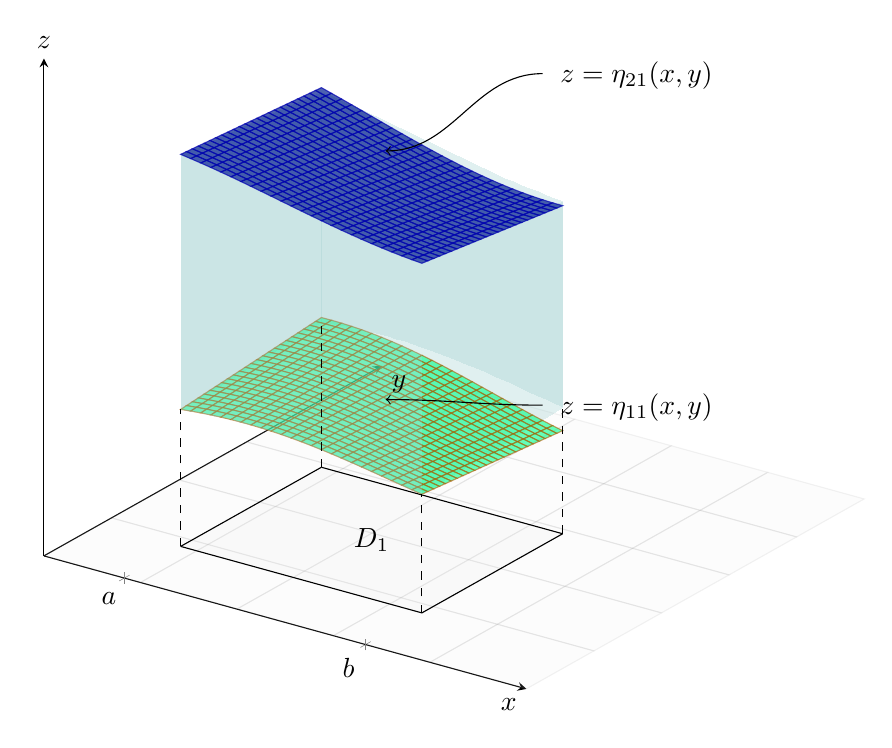
\begin{tikzpicture}
    \begin{axis}[
        view={35}{25}, % Ángulo de perspectiva
        width=12cm, height=12cm,
        grid=none,
        axis lines=center,
        xmin=0, xmax=6,
        ymin=0, ymax=6,
        zmin=0, zmax=6,
        xtick={1,4}, xticklabels={$a$,$b$}, % Marcas exactas de a y b en el eje x
        ytick=\empty, ztick=\empty,
        xlabel={$x$}, ylabel={$y$}, zlabel={$z$},
        every axis x label/.style={at={(ticklabel* cs:1)},anchor=north east},
        every axis y label/.style={at={(ticklabel* cs:1)},anchor=north west},
        every axis z label/.style={at={(ticklabel* cs:1)},anchor=south},
        clip=false
    ]

    % --- 0. Grilla en el piso (z=0) ---
    \addplot3 [surf, domain=0:6, domain y=0:6, samples=6, samples y=6, opacity=0.1, point meta=0, colormap={fondogris}{color=(gray!25) color=(gray!25)}, shader=faceted, faceted color=gray] (x,y,0);

    % --- 1. Dominio D_1 en R2 (Plano z=0) ---
    \addplot3 [surf, domain=1:4, domain y=0:1, samples=30, opacity=0.15, colormap={gray}{color=(gray!15) color=(gray!15)}, shader=interp, draw=none] 
        (x, {1 + 2.5*y}, 0);

    % Contorno de D1 (borde recto, uniendo las esquinas de la sombra)
    \draw[thin, black] (1, 1, 0) -- (4, 1, 0);
    \draw[thin, black] (1, 3.5, 0) -- (4, 3.5, 0);
    \draw[thin, black] (1, 1, 0) -- (1, 3.5, 0);
    \draw[thin, black] (4, 1, 0) -- (4, 3.5, 0);

    % --- 2. Paredes laterales (Efecto sólido) ---
    % Pared trasera
    \addplot3 [surf, domain=1:4, domain y=0:1, samples=30, opacity=0.3, colormap={teal}{color=(teal!40) color=(teal!40)}, shader=interp, draw=black!70] 
        (x, 3.5, { (1-y)*(1.5 + 0.2*sin(x*50) + 0.1) + y*(4.5 + 0.3*cos(x*40) - 0.2) });

    % Pared izquierda (en x=a)
    \addplot3 [surf, domain=0:1, domain y=0:1, samples=5, opacity=0.3, colormap={teal}{color=(teal!40) color=(teal!40)}, shader=interp, draw=black!70] 
        (1, {1 + 2.5*x}, { (1-y)*(1.5 + 0.2*sin(50) + 0.1*x) + y*(4.5 + 0.3*cos(40) - 0.2*x) });

    % Pared derecha (en x=b)
    \addplot3 [surf, domain=0:1, domain y=0:1, samples=5, opacity=0.3, colormap={teal}{color=(teal!40) color=(teal!40)}, shader=interp, draw=black!70] 
        (4, {1 + 2.5*x}, { (1-y)*(1.5 + 0.2*sin(200) + 0.1*x) + y*(4.5 + 0.3*cos(160) - 0.2*x) });

    % --- 3. Tapas del sólido ---
    % ¡AHORA SÍ!: Tapa inferior forzada a NARANJA plano con un mapa de color puro
    \addplot3 [surf, domain=1:4, domain y=0:1, samples=25, opacity=0.6, 
               colormap={pureorange}{rgb255=(0,255,140,0) rgb255=(1,255,140,0)}, shader=flat, draw=orange!70!black] 
        (x, {1 + 2.5*y}, { 1.5 + 0.2*sin(x*50) + 0.2*y*cos(x*40) });
        
    % Pared frontal
    \addplot3 [surf, domain=1:4, domain y=0:1, samples=30, opacity=0.3, colormap={teal}{color=(teal!40) color=(teal!40)}, shader=interp, draw=black!70] 
        (x, 1, { (1-y)*(1.5 + 0.2*sin(x*50)) + y*(4.5 + 0.3*cos(x*40)) });

    % Tapa superior forzada a AZUL plano con su propio mapa puro
    \addplot3 [surf, domain=1:4, domain y=0:1, samples=25, opacity=0.7, 
               colormap={pureblue}{rgb255=(0,30,144,255) rgb255=(1,30,144,255)}, shader=flat, draw=blue!70!black] 
        (x, {1 + 2.5*y}, { 4.5 + 0.3*cos(x*40) - 0.3*y*sin(x*30) });

    % --- 4. Esquinas y proyecciones (Líneas punteadas de soporte) ---
    \draw[dashed, thin] (1, 1, 0) -- (1, 1, {1.5 + 0.2*sin(50)});
    \draw[dashed, thin] (4, 1, 0) -- (4, 1, {1.5 + 0.2*sin(200)});
    \draw[dashed, thin] (1, 3.5, 0) -- (1, 3.5, {1.5 + 0.2*sin(50) + 0.1});
    \draw[dashed, thin] (4, 3.5, 0) -- (4, 3.5, {1.5 + 0.2*sin(200) + 0.1});

    % --- 5. Etiquetas ---
    \node at (2.5, 2.25, 0) {$D_1$};

    % Etiquetas de las superficies
    \node[anchor=west] at (3.5, 4, 5.2) {$z = \eta_{21}(x,y)$};
    \node[anchor=west] at (3.5, 4, 1.2) {$z = \eta_{11}(x,y)$};
    
    % Flechas a las superficies
    \draw[->, out=180, in=0, thin] (3.4, 4, 5.2) to (2.5, 2.5, 4.6);
    \draw[->, out=180, in=0, thin] (3.4, 4, 1.2) to (2.5, 2.5, 1.6);

\end{axis}
\end{tikzpicture}
\caption{Conjunto elemental de Tipo I.}
 
    \label{fig:conjunto tipo 1}
\end{figure}
\end{enumerate}
\end{definition}


\begin{itemize}
    \item Existen $D_2 \subset \mathbb{R}^2$ un conjunto elemental y funciones $\eta_{12},\; \eta_{22}: D_2\to\mathbb{R}$ continuas tales que 
    \[
    \eta_{12}(x, z) < \eta_{22}(x, z) \quad \forall (x,z) \in (D_2)^{\circ}
    \]
    y 
    \begin{equation}
        \label{def_conj_elem_R3_t2} 
        W = \left\{ (x, y, z) \in \mathbb{R}^3 \;\middle|\; (x,z) \in D_2 \: \land \: \eta_{12}(x, z) \leq y \leq \eta_{22}(x, z) \: \forall (x,z) \in D_2 \right\}
    \end{equation}
\end{itemize}

\begin{figure}[htbp]
    \centering
    % Llamamos al archivo con el código TikZ extraído
    \tikzexternaldisable
    \centering
    \tikzsetnextfilename{conj_elemental2_R3}
    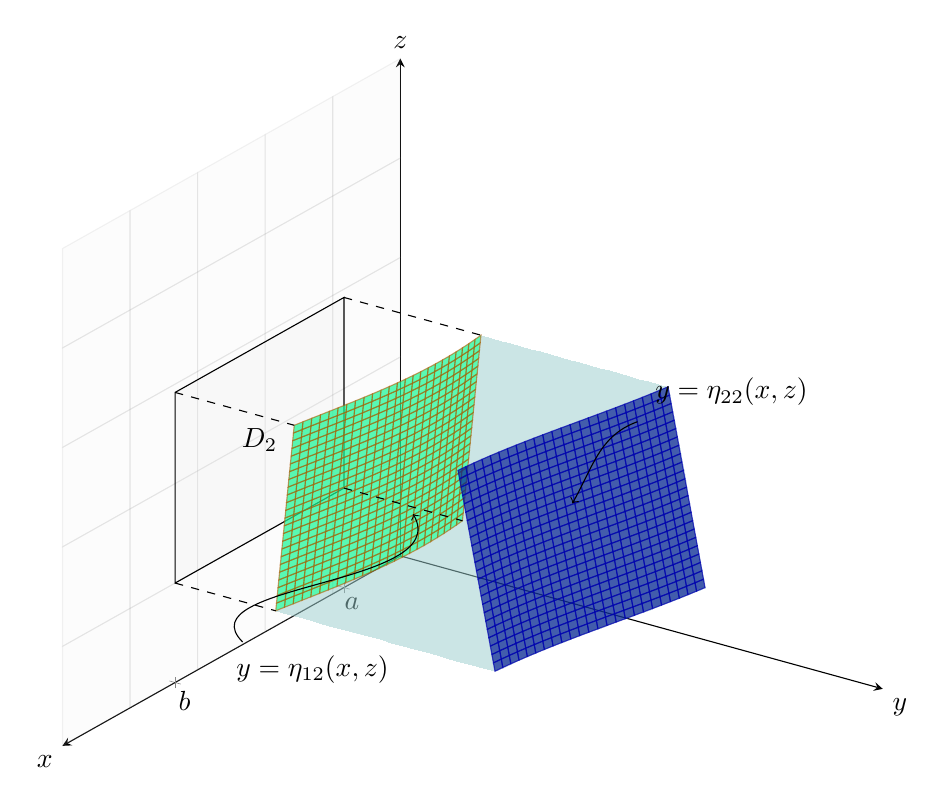
\begin{tikzpicture}
    \begin{axis}[
        view={125}{25}, % Rotado para que el sólido "venga" hacia adelante
        width=12cm, height=12cm,
        grid=none,
        axis lines=center,
        xmin=0, xmax=6,
        ymin=0, ymax=6, % Eje de profundidad y proyectado
        zmin=0, zmax=6,
        xtick={1,4}, xticklabels={$a$,$b$},
        ytick=\empty, ztick=\empty,
        xlabel={$x$}, ylabel={$y$}, zlabel={$z$},
        every axis x label/.style={at={(ticklabel* cs:1)},anchor=north east},
        every axis y label/.style={at={(ticklabel* cs:1)},anchor=north west},
        every axis z label/.style={at={(ticklabel* cs:1)},anchor=south},
        clip=false
    ]

    % --- 0. Grilla de fondo (plano xz en y=0) ---
    \addplot3 [surf, domain=0:6, domain y=0:6, samples=6, samples y=6, opacity=0.1, point meta=0, colormap={fondogris}{color=(gray!25) color=(gray!25)}, shader=faceted, faceted color=gray] (x,0,y);

    % --- 1. Dominio D_2 en R2 (Plano xz) ---
    % Relleno de D2
    \addplot3 [surf, domain=1:4, domain y=1.2:3.5, samples=2, opacity=0.15, colormap={gray}{color=(gray!20) color=(gray!20)}, shader=interp, draw=none] 
        (x, 0, y);
    % Contorno de D2 (borde recto)
    \draw[thin, black] (1, 0, 1.2) -- (4, 0, 1.2) -- (4, 0, 3.5) -- (1, 0, 3.5) -- cycle;

    % --- 2. Paredes del volumen (Relleno completo de las 4 caras laterales) ---
    % Pared en z = 3.5 (Toma en cuenta z=3.5 para cerrar perfecto con el techo)
    \addplot3 [surf, domain=1:4, domain y=0:1, samples=20, opacity=0.3, colormap={teal}{color=(teal!40) color=(teal!40)}, shader=interp, draw=black!70]
        (x, { (1-y)*(1.2 + 0.2*sin(x*50) + 0.1*3.5) + y*(4.5 + 0.3*cos(x*40) - 0.2*3.5) }, 3.5);
    % Pared en z = 1.2 (Toma en cuenta z=1.2 para cerrar perfecto con el techo)
    \addplot3 [surf, domain=1:4, domain y=0:1, samples=20, opacity=0.3, colormap={teal}{color=(teal!40) color=(teal!40)}, shader=interp, draw=black!70]
        (x, { (1-y)*(1.2 + 0.2*sin(x*50) + 0.1*1.2) + y*(4.5 + 0.3*cos(x*40) - 0.2*1.2) }, 1.2);
    % Pared en x = a (x=1)
    \addplot3 [surf, domain=1.2:3.5, domain y=0:1, samples=20, opacity=0.3, colormap={teal}{color=(teal!40) color=(teal!40)}, shader=interp, draw=black!70]
        (1, { (1-y)*(1.2 + 0.2*sin(50) + 0.1*x) + y*(4.5 + 0.3*cos(40) - 0.2*x) }, x);
    % Pared en x = b (x=4)
    \addplot3 [surf, domain=1.2:3.5, domain y=0:1, samples=20, opacity=0.3, colormap={teal}{color=(teal!40) color=(teal!40)}, shader=interp, draw=black!70]
        (4, { (1-y)*(1.2 + 0.2*sin(200) + 0.1*x) + y*(4.5 + 0.3*cos(160) - 0.2*x) }, x);

    % --- 3. Superficie Trasera y = eta12 ---
    \addplot3 [surf, domain=1:4, domain y=1.2:3.5, samples=25, opacity=0.6,
               colormap={pureorange}{rgb255=(0,255,140,0) rgb255=(1,255,140,0)}, shader=flat, draw=orange!70!black]
        (x, { 1.2 + 0.2*sin(x*50) + 0.1*y }, y);

    % --- 4. Superficie Delantera y = eta22 (Mirando al frente) ---
    \addplot3 [surf, domain=1:4, domain y=1.2:3.5, samples=25, opacity=0.7,
               colormap={pureblue}{rgb255=(0,30,144,255) rgb255=(1,30,144,255)}, shader=flat, draw=blue!70!black]
        (x, { 4.5 + 0.3*cos(x*40) - 0.2*y }, y);

    % --- 5. Proyecciones punteadas al plano (una por cada esquina de D2) ---
    \draw[dashed, thin] (1,0,1.2) -- (1, {1.2 + 0.2*sin(50) + 0.1*1.2}, 1.2);
    \draw[dashed, thin] (4,0,1.2) -- (4, {1.2 + 0.2*sin(200) + 0.1*1.2}, 1.2);
    \draw[dashed, thin] (1,0,3.5) -- (1, {1.2 + 0.2*sin(50) + 0.1*3.5}, 3.5);
    \draw[dashed, thin] (4,0,3.5) -- (4, {1.2 + 0.2*sin(200) + 0.1*3.5}, 3.5);

    % --- 6. Etiquetas y flechas (ajustadas para que no tapen la figura) ---
    \node at (2.5, 0, 2.35) {$D_2$};
    
    % Flecha para la cara delantera (techo)
    \node[anchor=south west] at (3.5, 5.5, 4.5) {$y = \eta_{22}(x,z)$};
    \draw[->, thin] (3.5, 5.4, 4.4) to[out=200, in=60] (2.8, 4.1, 2.8);
    
    % Flecha para la cara trasera (piso curvo)
    \node[anchor=north west] at (3.8, 0.5, 0.5) {$y = \eta_{12}(x,z)$};
    \draw[->, thin] (3.8, 0.7, 0.6) to[out=135, in=300] (2.2, 1.7, 1.8);

    \end{axis}
    \end{tikzpicture}
    \caption{Conjunto elemental de Tipo 2.}

 
    \label{fig:Conjunto tipo 2}
\end{figure}

\begin{itemize}
    \item Existen $D_3 \subset \mathbb{R}^2$ un conjunto elemental y funciones $\eta_{13},\; \eta_{23}: D_3\to\mathbb{R}$ continuas tales que 
    $$\eta_{13}(y, z) < \eta_{23}(y, z) \: \forall (y,z) \in (D_3)^{\circ}$$ 
    y 
    \begin{equation}
        \label{def_conj_elem_R3_t3} 
        W = \left\{ (x, y, z) \in \mathbb{R}^3 \;\middle|\; (y,z) \in D_3 \: \land \: \eta_{13}(y, z) \leq x \leq \eta_{23}(y, z) \: \forall (y,z) \in D_3 \right\} 
    \end{equation}
\end{itemize}
\begin{figure}[htbp]
    \centering
    % Llamamos al archivo con el código TikZ extraído
    
    \centering
    \tikzsetnextfilename{conj_elemental3_R3}
    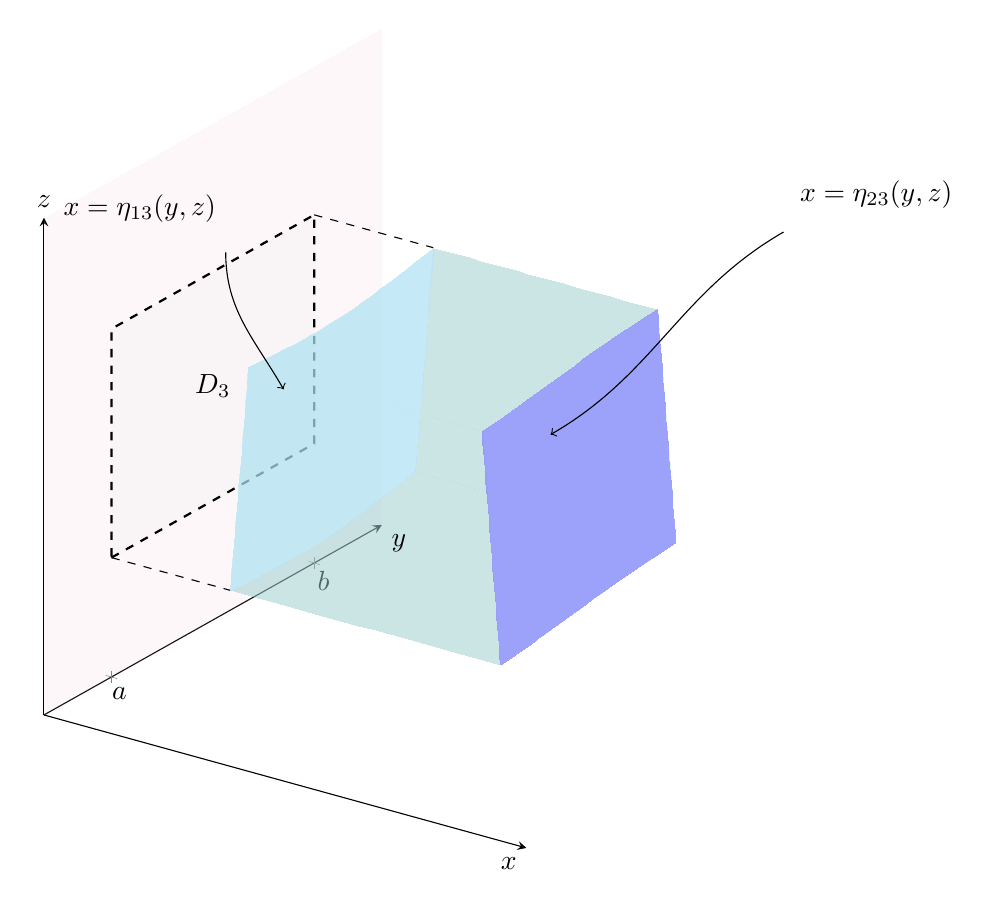
\begin{tikzpicture}
    \begin{axis}[
        view={35}{25}, 
        width=12cm, height=12cm,
        grid=none,
        axis lines=center,
        xmin=0, xmax=6, % Eje de proyección x
        ymin=0, ymax=5,
        zmin=0, zmax=5,
        xtick=\empty, ytick={1,4}, yticklabels={$a$,$b$},
        ztick=\empty,
        xlabel={$x$}, ylabel={$y$}, zlabel={$z$},
        every axis x label/.style={at={(ticklabel* cs:1)},anchor=north east},
        every axis y label/.style={at={(ticklabel* cs:1)},anchor=north west},
        every axis z label/.style={at={(ticklabel* cs:1)},anchor=south},
        clip=false
    ]

    % --- 0. Plano de fondo Lila (yz en x=0) ---
    \addplot3 [surf, domain=0:5, domain y=0:5, samples=2, opacity=0.1, colormap={lila}{color=(purple!30) color=(purple!30)}, shader=interp, draw=none] (0,x,y);

    % --- 1. Dominio D_3 en R2 (Plano yz) ---
    \addplot3 [surf, domain=1:4, domain y=1.2:3.5, samples=2, opacity=0.15, colormap={gray}{color=(gray!20) color=(gray!20)}, shader=interp, draw=none] 
        (0, x, y);
    \draw[dashed, black, thick] (0, 1, 1.2) -- (0, 4, 1.2) -- (0, 4, 3.5) -- (0, 1, 3.5) -- cycle;

    % --- 2. Paredes del volumen (Relleno completo de las 4 caras laterales) ---
    % Pared superior en z = 3.5
    \addplot3 [surf, domain=1:4, domain y=0:1, samples=20, opacity=0.3, colormap={teal}{color=(teal!40) color=(teal!40)}, shader=interp, draw=none] 
        ({ (1-y)*(1.2 + 0.2*sin(x*50) + 0.1*3.5) + y*(4.8 + 0.2*cos(x*40) - 0.1*3.5) }, x, 3.5);
    
    % Pared inferior en z = 1.2
    \addplot3 [surf, domain=1:4, domain y=0:1, samples=20, opacity=0.3, colormap={teal}{color=(teal!40) color=(teal!40)}, shader=interp, draw=none] 
        ({ (1-y)*(1.2 + 0.2*sin(x*50) + 0.1*1.2) + y*(4.8 + 0.2*cos(x*40) - 0.1*1.2) }, x, 1.2);

    % Pared lateral anterior en y = 1 (Une de z=1.2 a z=3.5)
    \addplot3 [surf, domain=1.2:3.5, domain y=0:1, samples=20, opacity=0.3, colormap={teal}{color=(teal!40) color=(teal!40)}, shader=interp, draw=none] 
        ({ (1-y)*(1.2 + 0.2*sin(1*50) + 0.1*x) + y*(4.8 + 0.2*cos(1*40) - 0.1*x) }, 1, x);

    % Pared lateral posterior en y = 4 (Une de z=1.2 a z=3.5)
    \addplot3 [surf, domain=1.2:3.5, domain y=0:1, samples=20, opacity=0.3, colormap={teal}{color=(teal!40) color=(teal!40)}, shader=interp, draw=none] 
        ({ (1-y)*(1.2 + 0.2*sin(4*50) + 0.1*x) + y*(4.8 + 0.2*cos(4*40) - 0.1*x) }, 4, x);

    % --- 3. Superficie Trasera x = eta13 ---
    \addplot3 [surf, domain=1:4, domain y=1.2:3.5, samples=25, opacity=0.6, colormap={cyan}{color=(cyan!30) color=(cyan!30)}, shader=interp, draw=none] 
        ({ 1.2 + 0.2*sin(x*50) + 0.1*y }, x, y);

    % --- 4. Superficie Delantera x = eta23 ---
    \addplot3 [surf, domain=1:4, domain y=1.2:3.5, samples=25, opacity=0.7, colormap={blue}{color=(blue!50) color=(blue!50)}, shader=interp, draw=none] 
        ({ 4.8 + 0.2*cos(x*40) - 0.1*y }, x, y);

    % --- 5. Proyecciones punteadas al plano ---
    \draw[dashed, thin] (0,1,1.2) -- ({1.2+0.2*sin(50)+0.1*1.2}, 1, 1.2);
    \draw[dashed, thin] (0,4,3.5) -- ({1.2+0.2*sin(200)+0.1*3.5}, 4, 3.5);

    % --- 6. Etiquetas y flechas optimizadas ---
    \node at (0, 2.5, 2.35) {$D_3$};
    
    % Flecha para la sábana frontal (azul)
    \node[anchor=south west] at (5.5, 4.5, 4.5) {$x = \eta_{23}(y,z)$};
    \draw[->, thin] (5.5, 4.4, 4.4) to[out=210, in=30] (4.2, 2.5, 2.8);
    
    % Flecha para la sábana trasera (cyan) - Desde arriba apuntando hacia abajo
    \node[anchor=south east] at (1.0, 1.5, 4.5) {$x = \eta_{13}(y,z)$};
    \draw[->, thin] (1.0, 1.5, 4.3) to[out=270, in=120] (1.3, 2.0, 2.8);

\end{axis}
\end{tikzpicture}
\caption{Conjunto elemental de Tipo 3.}
 
    \label{fig:Conjunto tipo 3}
\end{figure}



\newpage

\begin{example}
    Un ejemplo de un conjunto que es elemental en $\mathbb{R}^3$ es una esfera sólida (o bola) de radio $R$ centrada en el origen:
    $$W = \{(x,y,z) \in \mathbb{R}^3 \mid x^2 + y^2 + z^2 \leq R^2\}$$

    Para ver que es un conjunto elemental del primer tipo (proyección sobre el plano $xy$), identificamos primero su región de proyección $D_1$:
    $$D_1 = \{(x,y) \in \mathbb{R}^2 \mid x^2 + y^2 \leq R^2\}$$
    
    Sabemos que $D_1$ es un conjunto elemental en $\mathbb{R}^2$ (como se vio en el ejemplo de la Definición \ref{conj_elem}). Sobre esta región $D_1$, la variable $z$ queda acotada inferiormente por la semiesfera inferior y superiormente por la semiesfera superior. Es decir, existen las funciones continuas:
    $$ \eta_{11}(x,y) = -\sqrt{R^2 - x^2 - y^2} $$
    $$ \eta_{21}(x,y) = \sqrt{R^2 - x^2 - y^2} $$
    
    Tales que $\eta_{11}(x,y) \leq z \leq \eta_{21}(x,y)$ para todo $(x,y) \in D_1$. 

   Análogamente, se puede describir dicho conjunto de otras dos maneras según el plano en el que se proyecta:
\begin{enumerate}
    \item \textbf{Proyección sobre el plano $xz$:} La región elemental $D_2 \subset \mathbb{R}^2$ es el disco:
        \[
        D_2 = \{(x,z) \in \mathbb{R}^2 \mid x^2 + z^2 \leq R^2\}
        \]
        y la variable $y$ queda acotada por las funciones continuas:
        \[
        \eta_{12}(x,z) = -\sqrt{R^2 - x^2 - z^2} \quad \text{e} \quad \eta_{22}(x,z) = \sqrt{R^2 - x^2 - z^2}
        \]

    \item \textbf{Proyección sobre el plano $yz$:} La región elemental $D_3 \subset \mathbb{R}^2$ es el disco:
        \[
        D_3 = \{(y,z) \in \mathbb{R}^2 \mid y^2 + z^2 \leq R^2\}
        \]
        y la variable $x$ queda acotada por las funciones continuas:
        \[
        \eta_{13}(y,z) = -\sqrt{R^2 - y^2 - z^2} \quad \text{e} \quad \eta_{23}(y,z) = \sqrt{R^2 - y^2 - z^2}
        \]
\end{enumerate}

\begin{figure}[htbp]
    \centering
    % Llamamos al archivo con el código TikZ extraído
    
    \centering
 
    \tikzsetnextfilename{ej_esfera_elemental} 
    
    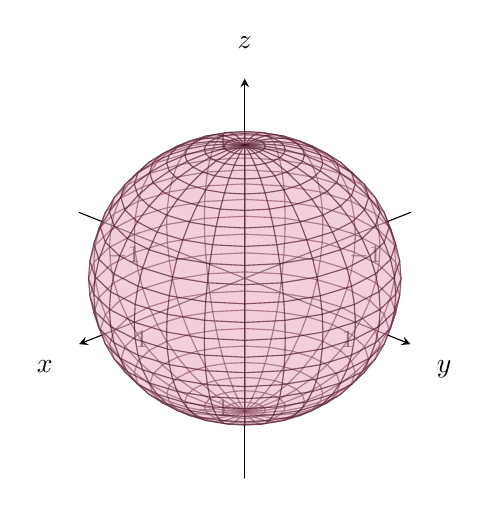
\begin{tikzpicture}[line cap=round, line join=round]
        \begin{axis}[
            view={135}{25}, % Cámara clásica
            width=10cm,
            height=10cm,
            axis lines=center,
            % Ajustamos los ejes a la esfera de radio 1
            xmin=-1.5, xmax=1.5, 
            ymin=-1.5, ymax=1.5,
            zmin=-1.5, zmax=1.5,
            xlabel={$x$},
            ylabel={$y$},
            zlabel={$z$},
            % Anclaje perfecto de letras
            every axis x label/.style={at={(ticklabel* cs:1.05)},anchor=north east},
            every axis y label/.style={at={(ticklabel* cs:1.05)},anchor=north west},
            every axis z label/.style={at={(ticklabel* cs:1.05)},anchor=south},
            ticklabel style={font=\small},
        ]

        % Esfera unitaria x^2 + y^2 + z^2 = 1 (Roja transparente)
        \addplot3[
            surf,
            opacity=0.4,
            color=purple!30,
            faceted color=purple!30!black,
            samples=25, % Reducido para no saturar la memoria
            domain=0:360,
            y domain=0:180,
            z buffer=sort
        ]
        ({cos(x)*sin(y)}, {sin(x)*sin(y)}, {cos(y)});

        \end{axis}
    \end{tikzpicture}
    \caption{Representación de la región $W$.}

 
    \label{fig:Representación de la región W}
\end{figure}
\end{example}



         \subsection{Teorema de Fubini}
             \begin{theorem} \label{teo:fubini_r3} \textbf{Teorema de Fubini} en $\mathbb{R}^3.$
    Sea $f:W\to\mathbb{R}$ un campo escalar continuo sobre $W\subseteq\mathbb{R}^3$ un conjunto elemental.
    
    \begin{enumerate} 
        \item Si $W$ es un conjunto de \textbf{Tipo 1}  (\ref{def_conj_elem_R3_t1}), entonces la integral triple de $f$ sobre $W$ se puede calcular como:
        \[
            \iiint_W f(x,y,z) \, dV = \iint_{D_1} \left( \int_{\eta_{11}(x,y)}^{\eta_{21}(x,y)} f(x,y,z) \, dz \right) dA
        \]
       
        \item Si $W$ es un conjunto de \textbf{Tipo 2} (\ref{def_conj_elem_R3_t2}), entonces la integral triple de $f$ sobre $W$ se puede calcular como:
        \[
            \iiint_W f(x,y,z) \, dV = \iint_{D_2} \left( \int_{\eta_{12}(x,z)}^{\eta_{22}(x,z)} f(x,y,z) \, dy \right) dA
        \]
       
 \item Si $W$ es un conjunto de \textbf{Tipo 3} (\ref{def_conj_elem_R3_t3}), entonces la integral triple de $f$ sobre $W$ se puede calcular como:
        \[
            \iiint_W f(x,y,z) \, dV = \iint_{D_3} \left( \int_{\eta_{13}(y,z)}^{\eta_{23}(y,z)} f(x,y,z) \, dx \right) dA
        \]
    \end{enumerate}
\end{theorem}





         \subsection{Teorema del Valor Medio Integral}
                 \input{capitulos/TVM_integral_r3.tex}
              
         \subsection{Teorema de Cambio de Variables en $\mathbb{R}^{3}$}
               \begin{definition}
    Sea $\mathbf{T}:A\subseteq\Rn{3}\to\Rn{3}$ un campo vectorial de clase  $\mathcal{C}^1(A)$ y sea $\boldsymbol{D}_\mathbf{T}$ (\autoref{def:mat_dif}) su matriz diferencial.  Se define el \emph{jacobiano}, o \emph{determinante jacobiano}, y se lo nota $J_\mathbf{T}$ al determinante de la matriz $\boldsymbol{D}_\mathbf{T}$, es decir,  
    \[
        J_\mathbf{T}=\text{det}(\boldsymbol{D}_\mathbf{T}).
    \]
\end{definition}





\begin{theorem}
\label{teo:cambio_variable}    
    \textbf{Teorema del cambio de variables para integrales triples.}  Sean $W \subseteq\Rn{3}$ un conjunto acotado y  $f:W \to\R$ un campo integrable sobre $W$ y sea $\mathbf{T}:W^*\subseteq\Rn{3}\to W\subseteq\Rn{3}$ continua en $W^*$, de clase $\mathcal{C}^1(\interior{(W^*)})$,  inyectiva en $\interior{(W^*)}$ y tal que $\mathbf{T}(W^*)=W$.  Entonces
    \[
        \iiint_W f\:dV=\iiint_{W^*}(f\circ\mathbf{T})J_\mathbf{T}\:dV.
    \]
\end{theorem}



               \subsection{Coordenadas Esfericas}
               
\label{sec:coordenadas_esfericas}


\textbf{Cambio de coordenadas Lineales} \textcolor{red}{Agregar}

Para el cálculo de integrales en regiones con simetría esf\'ericas, se utiliza el sistema de coordenadas esf\'ericas. Un punto $(x, y, z)$ se relaciona con $(\rho, \theta ,  \phi)$ mediante:
\begin{equation}\label{def:coord_esfericas}
\mathbf{T}:W^*=[0,R]\times[0, 2\pi]\times[0,\pi]  \subseteq\Rn{3} \to W\: : \: \mathbf{T}(r, \theta,z ) =( \rho \sin \phi \cos \theta  ,  \rho \sin \phi \sin \theta ,  \rho \cos \phi ).
\end{equation} 

\begin{tarea} Probar que la transformaci\'on $T$ definida en (\ref{def:coord_esfericas}) est\'a bajo las las hi\'otesis del Teorema  ~\ref{teo:cambio_variable}
\end{tarea}


Para el c\'alculo del \emph{Determinante Jacobiano} de $T$  primero  calculamos su  matriz diferencial $D_\mathbf{T}$, quedando
 
\[
    \boldsymbol{D}_{\mathbf{F}}(\rho, \theta, \phi) 
    =
    \begin{pmatrix}
    \sin\phi \cos\theta & -\rho \sin\phi \sin\theta & \rho \cos\phi \cos\theta \\
    \sin\phi \sin\theta & \rho \sin\phi \cos\theta & \rho \cos\phi \sin\theta \\
    \cos\phi & 0 & -\rho \sin\phi
    \end{pmatrix}
    \]
 
 por \'ultimo,  en nuestro caso,  como $  0 \leq \phi \leq \pi$, tenemos
\begin{equation}   \label{ej:jacobiano_esferico}
    \left| J_{\mathbf{T}} \right| = \rho^2 \sin \phi
\end{equation}
  
\textbf{Visualización del sistema de coordenadas esféricas}

\begin{figure}[H]
    \centering
    % Llamamos al archivo con el código TikZ extraído
    
    \centering
    \tikzsetnextfilename{esfericas_cambio_figura}

    \begin{tikzpicture}

    %%% IZQUIERDA: caja W* en espacio (ρ, φ, θ)
    \begin{axis}[
        name=izq,
        view={110}{25},
        width=7cm,
        height=7cm,
        xmin=-0.2, xmax=3.5,
        ymin=-0.2, ymax=7.5,
        zmin=-0.2, zmax=3.8,
        xlabel={$\rho$},
        ylabel={$\theta$},
        zlabel={$\phi$},
        axis lines=center,
        ticks=none,
        every axis x label/.style={at={(ticklabel* cs:1.05)}, anchor=north east},
        every axis y label/.style={at={(ticklabel* cs:1.05)}, anchor=north west},
        every axis z label/.style={at={(ticklabel* cs:1.05)}, anchor=south},
    ]

    % Cara inferior (φ = 0)
    \addplot3[fill=magenta!20, opacity=0.85, draw=magenta!70, thick]
        coordinates {(0,0,0)(3,0,0)(3,6.28,0)(0,6.28,0)(0,0,0)};
    % Cara posterior (θ = 0)
    \addplot3[fill=magenta!15, opacity=0.7, draw=magenta!70, thick]
        coordinates {(0,0,0)(3,0,0)(3,0,3.14)(0,0,3.14)(0,0,0)};
    % Cara lateral (ρ = 0)
    \addplot3[fill=magenta!20, opacity=0.7, draw=magenta!70, thick]
        coordinates {(0,0,0)(0,6.28,0)(0,6.28,3.14)(0,0,3.14)(0,0,0)};
    % Cara frontal (ρ = R)
    \addplot3[fill=magenta!30, opacity=0.8, draw=magenta!70, thick]
        coordinates {(3,0,0)(3,6.28,0)(3,6.28,3.14)(3,0,3.14)(3,0,0)};
    % Cara lateral (θ = 2π)
    \addplot3[fill=magenta!25, opacity=0.75, draw=magenta!70, thick]
        coordinates {(0,6.28,0)(3,6.28,0)(3,6.28,3.14)(0,6.28,3.14)(0,6.28,0)};
    % Cara superior (φ = π)
    \addplot3[fill=magenta!35, opacity=0.9, draw=magenta!70, thick]
        coordinates {(0,0,3.14)(3,0,3.14)(3,6.28,3.14)(0,6.28,3.14)(0,0,3.14)};

    % Etiqueta W*
    \node[color=magenta!80!black, font=\Large]
        at (axis cs: 1.5, 3.14, 1.57) {$W^*$};

    % Cotas
    \node[below, color=black!60, font=\small]
        at (axis cs: 3, 0, 0) {$R$};
    \node[above right, color=black!60, font=\small]
        at (axis cs: 0, 6.28, 0) {$2\pi$};
    \node[left, color=black!60, font=\small]
        at (axis cs: 0, 0, 0) {$0$};
    \node[left, color=black!60, font=\small]
        at (axis cs: 0, 0, 3.14) {$\pi$};

    \end{axis}

    % Label inferior izquierdo
    \node[below=0.15cm of izq.south, font=\small]
        {Espacio $(\rho,\theta,\phi)$};

    %%% FLECHA T
    \draw[-{Stealth[length=9pt, width=6pt]}, thick]
        ($(izq.east)+(0.4,0)$)
        -- node[above, font=\large]{$T$}
        ++(1.5,0);

    %%% DERECHA: esfera W en espacio (x, y, z)
    \begin{axis}[
        name=der,
        at={($(izq.east)+(2.4cm,0)$)},
        anchor=west,
        view={110}{25},
        unit vector ratio=1 1 1,
        width=7cm,
        height=7cm,
        xmin=-3, xmax=3,
        ymin=-3, ymax=3,
        zmin=-3, zmax=3,
        xlabel={$x$},
        ylabel={$y$},
        zlabel={$z$},
        axis lines=center,
        ticks=none,
        every axis x label/.style={at={(ticklabel* cs:1.05)}, anchor=north east},
        every axis y label/.style={at={(ticklabel* cs:1.05)}, anchor=north west},
        every axis z label/.style={at={(ticklabel* cs:1.05)}, anchor=south},
    ]

    % Hemisferio inferior
    \addplot3[surf, draw=green!45,
              point meta=0, colormap={verdeinf}{color=(green!20) color=(green!20)},
              fill opacity=0.32, draw opacity=0.75,
              domain=0:360, y domain=90:180,
              samples=48, samples y=22, shader=interp]
        ({2*cos(x)*sin(y)}, {2*sin(x)*sin(y)}, {2*cos(y)});

    % Hemisferio superior
    \addplot3[surf, draw=green!55,
              point meta=0, colormap={verdesup}{color=(green!30) color=(green!30)},
              fill opacity=0.38, draw opacity=0.85,
              domain=0:360, y domain=0:90,
              samples=48, samples y=22, shader=interp]
        ({2*cos(x)*sin(y)}, {2*sin(x)*sin(y)}, {2*cos(y)});

    % Circulo ecuatorial (z = 0)
    \addplot3[draw=green!70, thick, domain=0:360, samples=60]
        ({2*cos(x)}, {2*sin(x)}, {0});

    % Etiqueta W
    \node[color=green!50!black, font=\Large]
        at (axis cs: 0.4, 0.4, 0.8) {$W$};

    \end{axis}

    % Label inferior derecho
    \node[below=0.15cm of der.south, font=\small]
        {Espacio $(x,y,z)$};

    \end{tikzpicture}

    \caption{Visualización del sistema de coordenadas esféricas. 
    El bloque $W^*$ a la izquierda representa la región en el espacio 
    $(\rho,\theta,\phi)$ con sus límites típicos, mientras que la esfera 
    $W$ a la derecha muestra cómo se transforma esa región en el 
    espacio $(x,y,z)$ mediante la transformación $T$.\href{https://www.geogebra.org/m/pzujyjqy}{Ver en GeoGebra }}
 
    \label{fig:Visualizacion esfericas}
\end{figure}

\vspace{1cm}


             \subsection{Coordenadas Cilindricas}
               
\label{sec:cilindricas}
\vspace{0.2cm}

Para el cálculo de integrales en regiones con simetría cilíndrica, se utiliza el sistema de coordenadas cilíndricas. Un punto $(x, y, z)$ se relaciona con $(r, \theta, z)$ mediante:

\begin{equation}\label{def:coord_cilindricas}
\mathbf{T}:W^*=[0,R]\times[0, 2\pi]\times[0,H] \subseteq\Rn{3} \to W\: : \: \mathbf{T}(r, \theta,z ) =( r \cos \theta , r \sin \theta,z ).
\end{equation} 

\begin{tarea} Probar que la transformaci\'on $T$ definida en (\ref{def:coord_cilindricas}) est\'a bajo las las hi\'otesis del Teorema  ~\ref{teo:cambio_variable}
\end{tarea}

\vspace{0.2cm}

Para el c\'alculo del \emph{Determinante Jacobiano} de $T$  primero  calculamos su  matriz diferencial $D_\mathbf{T}$, quedando
       \begin{equation*}
       \boldsymbol{D}_{\mathbf{T}}(r, \theta,z ) 
       =
       \begin{pmatrix}
       \cos\theta & -r\sin\theta & 0 \\
       \sin\theta & r\cos\theta & 0 \\
       0 & 0 & 1
       \end{pmatrix}
 \end{equation*}
 luego, el jacobiano es
       \begin{equation}\label{ejemplo_jacobiano_polares}
       J_{\mathbf{T}}(r, \theta,z) = \det(\boldsymbol{D}_{\mathbf{T}})(r, \theta,z) = 
      r(\cos^2\theta + \sin^2\theta) = r,
      \end{equation} 
 por \'ultimo,  en nuestro caso,  como $r \geq 0$, tenemos
\begin{equation}
|J_{\mathbf{T}}| = r
\end{equation}

\textbf{Visualización del sistema de coordenadas cilíndricas}

\begin{figure}[H]
    \centering
    \tikzsetnextfilename{cilindricas_cambio_figura}

    \begin{tikzpicture}

    %%% IZQUIERDA: caja W* en espacio (r, θ, z)
    \begin{axis}[
        name=izq,
        view={110}{25},
        width=7cm,
        height=7cm,
        xmin=-0.2, xmax=3,
        ymin=-0.2, ymax=7.5,
        zmin=-0.2, zmax=3,
        xlabel={$r$},
        ylabel={$\theta$},
        zlabel={$z$},
        axis lines=center,
        ticks=none,
        every axis x label/.style={at={(ticklabel* cs:1.05)}, anchor=north east},
        every axis y label/.style={at={(ticklabel* cs:1.05)}, anchor=north west},
        every axis z label/.style={at={(ticklabel* cs:1.05)}, anchor=south},
    ]

    % Cara inferior (z = 0)
    \addplot3[fill=magenta!20, opacity=0.85, draw=magenta!70, thick]
        coordinates {(0,0,0)(2.5,0,0)(2.5,6.28,0)(0,6.28,0)(0,0,0)};
    % Cara posterior (θ = 0)
    \addplot3[fill=magenta!15, opacity=0.7, draw=magenta!70, thick]
        coordinates {(0,0,0)(2.5,0,0)(2.5,0,2.5)(0,0,2.5)(0,0,0)};
    % Cara lateral (r = 0)
    \addplot3[fill=magenta!20, opacity=0.7, draw=magenta!70, thick]
        coordinates {(0,0,0)(0,6.28,0)(0,6.28,2.5)(0,0,2.5)(0,0,0)};
    % Cara frontal (r = 2.5)
    \addplot3[fill=magenta!30, opacity=0.8, draw=magenta!70, thick]
        coordinates {(2.5,0,0)(2.5,6.28,0)(2.5,6.28,2.5)(2.5,0,2.5)(2.5,0,0)};
    % Cara lateral (θ = 2π)
    \addplot3[fill=magenta!25, opacity=0.75, draw=magenta!70, thick]
        coordinates {(0,6.28,0)(2.5,6.28,0)(2.5,6.28,2.5)(0,6.28,2.5)(0,6.28,0)};
    % Cara superior (z = 2.5)
    \addplot3[fill=magenta!35, opacity=0.9, draw=magenta!70, thick]
        coordinates {(0,0,2.5)(2.5,0,2.5)(2.5,6.28,2.5)(0,6.28,2.5)(0,0,2.5)};

    % Etiqueta W*
    \node[color=magenta!80!black, font=\Large]
        at (axis cs: 1.25, 3.14, 1.25) {$W^*$};

    % Cotas
    \node[below, color=black!60, font=\small]
       at (axis cs: 2.5, 0, 0) {$R$};
    \node[above right, color=black!60, font=\small]
        at (axis cs: 0, 6.28, 0) {$2\pi$};
    \node[left, color=black!60, font=\small]
        at (axis cs: 0, 0, 0) {$z_1$};
    \node[left, color=black!60, font=\small]
        at (axis cs: 0, 0, 2.5) {$H$};

    \end{axis}

    % Label inferior izquierdo
    \node[below=0.15cm of izq.south, font=\small]
        {Espacio $(r,\theta,z)$};

    %%% FLECHA T
    \draw[-{Stealth[length=9pt, width=6pt]}, thick]
        ($(izq.east)+(0.4,0)$)
        -- node[above, font=\large]{$T$}
        ++(1.5,0);

    %%% DERECHA: cilindro W en espacio (x, y, z)
    \begin{axis}[
        name=der,
        at={($(izq.east)+(2.4cm,0)$)},
        anchor=west,
        view={110}{25},
        width=7cm,
        height=7cm,
        xmin=-2.8, xmax=2.8,
        ymin=-2.8, ymax=2.8,
        zmin=-0.2, zmax=3,
        xlabel={$x$},
        ylabel={$y$},
        zlabel={$z$},
        axis lines=center,
        ticks=none,
        every axis x label/.style={at={(ticklabel* cs:1.05)}, anchor=north east},
        every axis y label/.style={at={(ticklabel* cs:1.05)}, anchor=north west},
        every axis z label/.style={at={(ticklabel* cs:1.05)}, anchor=south},
    ]

    % Disco inferior (z = 0)
    \addplot3[surf, fill=green!25, draw=green!55,
              fill opacity=0.8, draw opacity=0.9,
              domain=0:360, y domain=0:2,
              samples=36, samples y=3, shader=flat]
        ({y*cos(x)}, {y*sin(x)}, {0});

    % Superficie lateral
    \addplot3[surf, fill=green!20, draw=green!45,
              fill opacity=0.65, draw opacity=0.8,
              domain=0:360, y domain=0:2.5,
              samples=36, samples y=10, shader=flat]
        ({2*cos(x)}, {2*sin(x)}, {y});

    % Disco superior (z = 2.5)
    \addplot3[surf, fill=green!35, draw=green!60,
              fill opacity=0.9, draw opacity=1,
              domain=0:360, y domain=0:2,
              samples=36, samples y=3, shader=flat]
        ({y*cos(x)}, {y*sin(x)}, {2.5});

    % Etiqueta W
    \node[color=green!50!black, font=\Large]
        at (axis cs: 0.5, 0.5, 1.25) {$W$};

    \end{axis}

    % Label inferior derecho
    \node[below=0.15cm of der.south, font=\small]
        {Espacio $(x,y,z)$};

    \end{tikzpicture}

    \caption{Visualización del sistema de coordenadas cilíndricas. 
    El bloque $W^*$ a la izquierda representa la región en el espacio 
    $(r,\theta,z)$ con sus límites típicos, mientras que el cilindro 
    $W$ a la derecha muestra cómo se transforma esa región en el 
    espacio $(x,y,z)$ mediante la transformación $T$. \href{https://www.geogebra.org/m/yam9nnxq}{Ver en GeoGebra }}

\end{figure}
          
         \subsection{Ejemplos}
         
\begin{example}
Sea $W$ el sólido limitado por el cilindro parabólico $y = x^2$ y los planos $z = 0$, $z = 4$ y $y = 1$. Calcular $\iiint_W yz \: dV$. 
\end{example}


\textbf{Soluci\'on:}
\begin{figure}[htbp]
    \centering
    % Llamamos al archivo con el código TikZ extraído
    \begin{center}
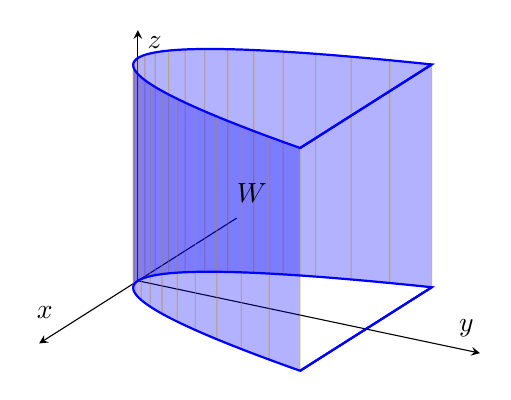
\begin{tikzpicture}
    \begin{axis}[
        view={120}{30},
        axis lines=center,
        xlabel=$x$, ylabel=$y$, zlabel=$z$,
        xmin=-1.5, xmax=1.5, ymin=0, ymax=1.5, zmin=0, zmax=4.5,
        ticks=none,
        clip=false
    ]
        % Superficie lateral y=x^2
        \addplot3[surf, opacity=0.3, blue, domain=-1:1, y domain=0:4, samples=25, samples y=2] (x, {x^2}, y);
        
        % Líneas de contorno para dar definición
        \addplot3[thick, blue, domain=-1:1, samples=50] (x, {x^2}, 0);
        \addplot3[thick, blue, domain=-1:1, samples=50] (x, {x^2}, 4);
        \draw[thick, blue] (axis cs:-1,1,0) -- (axis cs:1,1,0);
        \draw[thick, blue] (axis cs:-1,1,4) -- (axis cs:1,1,4);
        
        \node at (axis cs:0,0.5,2) {$W$};
    \end{axis}
\end{tikzpicture}
\end{center} 
    \label{fig:ejemplo 8.2.2}
\end{figure}

La región $W$ puede describirse como:
\[
    W = \{ (x,y,z) \in \Rn{3} : -1 \leq x \leq 1; \; x^2 \leq y \leq 1; \; 0 \leq z \leq 4 \}.
\]
Aplicando el Teorema de Fubini:
\begin{gather*}
    \iiint_W yz \: dV = \int_{-1}^{1} \int_{x^2}^{1} \int_{0}^{4} yz \: dz \, dy \, dx = \int_{-1}^{1} \int_{x^2}^{1} y \left[ \frac{z^2}{2} \right]_0^4 dy \, dx \\
    = \int_{-1}^{1} \int_{x^2}^{1} 8y \: dy \, dx = 8 \int_{-1}^{1} \left[ \frac{y^2}{2} \right]_{x^2}^1 dx = 4 \int_{-1}^{1} (1 - x^4) \: dx \\
    = 4 \left[ x - \frac{x^5}{5} \right]_{-1}^1 = 4 \left( \left( 1 - \frac{1}{5} \right) - \left( -1 + \frac{1}{5} \right) \right) = 4 \left( \frac{4}{5} + \frac{4}{5} \right) = \frac{32}{5}.
\end{gather*}


\clearpage

\begin{example}  Hallar el volumen del cuerpo $W$  dentro de la esfera  \(x^2+y^2+z^2=32\)  tal que
\(z \geq \sqrt{x^2+y^2}\).
\end{example}

\begin{figure}[htbp]
    \centering
    % Llamamos al archivo con el código TikZ extraído
    \begin{figure}[H]
    \centering
    \tikzsetnextfilename{ejercicio30_figura} 

    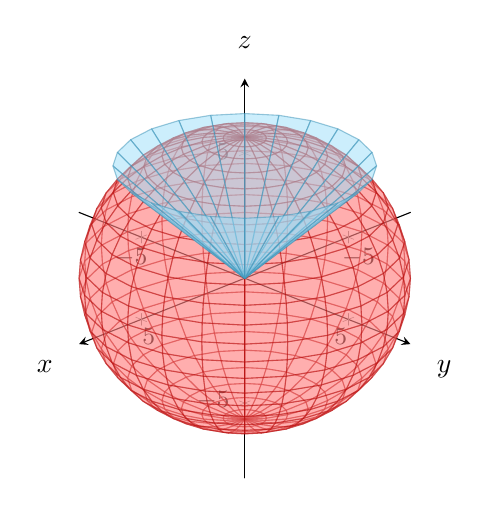
\begin{tikzpicture}[line cap=round, line join=round]
        \begin{axis}[
            view={135}{25}, % Cámara clásica
            width=10cm,
            height=10cm,
            axis lines=center,
            % 1. Ajustamos los ejes al nuevo tamaño de la esfera (aprox 5.65)
            xmin=-8, xmax=8, 
            ymin=-8, ymax=8,
            zmin=-8, zmax=8,
            xlabel={$x$},
            ylabel={$y$},
            zlabel={$z$},
            every axis x label/.style={at={(ticklabel* cs:1.05)},anchor=north east},
            every axis y label/.style={at={(ticklabel* cs:1.05)},anchor=north west},
            every axis z label/.style={at={(ticklabel* cs:1.05)},anchor=south},
            ticklabel style={font=\small},
        ]

        % Esfera de radio \sqrt{32} (Roja transparente)
        \addplot3[
            surf,
            opacity=0.4,
            color=red!50,
            faceted color=red!70!black,
            samples=25, 
            domain=0:360,
            y domain=0:180,
            z buffer=sort
        ]
        ({sqrt(32)*cos(x)*sin(y)}, {sqrt(32)*sin(x)*sin(y)}, {sqrt(32)*cos(y)});

        % Cono Superior z = \sqrt{x^2+y^2} (Celeste transparente)
        \addplot3[
            surf,
            opacity=0.5,
            color=cyan!40,
            faceted color=cyan!70!black,
            samples=25,
            samples y=2, 
            domain=0:360,
            % 2. El cono se interseca en z=4. Le damos hasta 4.5 para que lo atraviese bien
            y domain=0:4.5, 
            z buffer=sort
        ]
        ({y*cos(x)}, {y*sin(x)}, {y});

        \end{axis}
    \end{tikzpicture}
    \caption{Representación de la región pedida. \href{https://www.geogebra.org/m/pvzc3wke}{Ver en GeoGebra}}
    \label{fig:ejercicio30_figura}
\end{figure} 
    \label{fig:Ejemplo 8.2.3}
\end{figure}


\textbf{Soluci\'on:} La superficies $x^2+y^2+z^2=32$  y  $z=\sqrt{x^2+y^2}$ son,  una esfera de radio \(R=4\sqrt{2}\)    y un semicono superior, respectivamente, como se muestra en la figura~\ref{fig:ejercicio30_figura}. 


Plantearemos  la soluci\'on del problema con distintos cambios de cooredenadas. 



La intersección entre  ambas superficies se obtiene de
\[
r=z, \quad r^2+z^2=32 \Rightarrow 2r^2=32 \Rightarrow r=4.
\]

\textbf{1. Coordenadas cartesianas:} El s\'olido  $W$ cumple que
\[
x^2+y^2+z^2 \le 32, \quad z \ge \sqrt{x^2+y^2},
\] podemos describirlo por
\[
W=\left\{(x,y,z):
-4  \le x\le 4,\;
-\sqrt{16-x^2}\le y\le \sqrt{16-x^2},\;
\sqrt{x^2+y^2}\le z\le \sqrt{32-x^2-y^2}
\right\}
\]luego,  \[
Vol (W)=\int_{-4}^{4}
\int_{-\sqrt{16-x^2}}^{\sqrt{16-x^2}}
\int_{\sqrt{x^2+y^2}}^{\sqrt{32-x^2-y^2}}
dz\,dy\,dx.
\]

\bigskip

\textbf{2. Coordenadas cilíndricas:} Usando la transformación en coordenadas cilíndricas (~\ref{def:coord_cilindricas}), el s\'olido $W$ podemos describirlo por
\[
W=\left\{(r,\theta,z):
0 \le \theta \le 2\pi,\;
0 \le r \le 4,\;
r \le z \le \sqrt{32-r^2}
\right\}
\]luego,
\[
Vol (W)=\int_{0}^{2\pi}
\int_{0}^{4}
\int_{r}^{\sqrt{32-r^2}}
r \, dz\,dr\,d\theta.
\]

\bigskip


\textbf{3. Coordenadas esféricas:} Usando la transformación en coordenadas esféricas (~\ref{def:coord_esfericas}), el s\'olido $W$ podemos describirlo por
\[
W=\left\{(\rho,\theta,\varphi):
0 \le \theta \le 2\pi,\;
0 \le \varphi \le \frac{\pi}{4},\;
0 \le \rho \le 4\sqrt{2}
\right\}
\]luego,
\[
Vol (W)=\int_{0}^{2\pi}
\int_{0}^{\pi/4}
\int_{0}^{4\sqrt{2}}
\rho^2\sin\varphi \, d\rho\,d\varphi\,d\theta.
\]

\bigskip
Calculando la integral triple en coordenadas esféricas:
\[
Vol(W) = \int_{0}^{2\pi} d\theta \cdot \int_{0}^{\pi/4} \sin\varphi \, d\varphi \cdot \int_{0}^{4\sqrt{2}} \rho^2 \, d\rho.
\]
Resolviendo cada integral iterada de forma independiente:
\[
\int_{0}^{2\pi} d\theta = 2\pi,
\]
\[
\int_{0}^{\pi/4} \sin\varphi \, d\varphi = \Big[ -\cos\varphi \Big]_{0}^{\pi/4} = -\frac{\sqrt{2}}{2} - (-1) = 1 - \frac{\sqrt{2}}{2},
\]
\[
\int_{0}^{4\sqrt{2}} \rho^2 \, d\rho = \left[ \frac{\rho^3}{3} \right]_{0}^{4\sqrt{2}} = \frac{(4\sqrt{2})^3}{3} = \frac{128\sqrt{2}}{3}.
\]
Multiplicando los tres resultados:
\[
Vol(W) = 2\pi \cdot \left(1 - \frac{\sqrt{2}}{2}\right) \cdot \frac{128\sqrt{2}}{3} = \frac{256\sqrt{2}\pi}{3} \left(1 - \frac{\sqrt{2}}{2}\right) = \frac{256\pi}{3}(\sqrt{2}-1).
\]

\[
\boxed{Vol(W) = \frac{256\pi}{3}(\sqrt{2}-1)}
\]
         \textbf{Ejercicio 27:} Calcular el volumen de la región limitada por $x^2 + y^2 = 2ax$, $x^2 + y^2 = az$ y $z = 0$ con $a \in \mathbb{R} \setminus \{0\}$.

Para calcular el volumen de una región sólida $W$, partimos de la definición 2.5.6:

\begin{equation}
    V = \iiint_{W} 1 \, dV
\end{equation}

Previo a integrar, resulta conveniente identificar las distintas superficies que conforman la frontera de $W$, teniendo en cuenta que las mismas dependen del parametro $a$:
\begin{itemize}
    \item \textbf{Cilindro:} $x^2 + y^2 = 2ax \implies (x-a)^2 + y^2 = a^2$. Es un cilindro circular de radio $|a|$ con centro en $(a,0)$.
    \item \textbf{Paraboloide:} $z = \frac{x^2 + y^2}{a}$. Es la superficie que limita la altura del sólido. Para valores de $a > 0$ el paraboloide es el techo de la superficie mientras que para valores de $a < 0$ es el piso de la superficie. 
    \item \textbf{Plano $xy$:} $z = 0$.
\end{itemize}


\begin{figure}[htbp]
    \centering
    % ESTA LÍNEA es la que crea el PDF en la carpeta /tikz
    \tikzsetnextfilename{ejercicio27_figura} 
    
    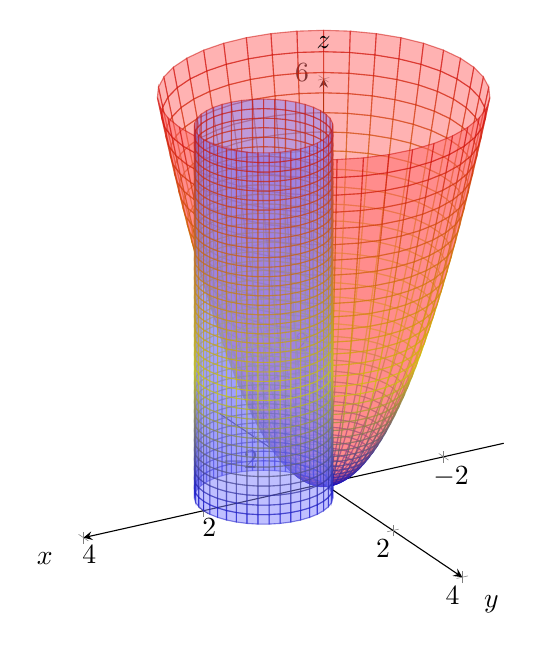
\begin{tikzpicture}
        \begin{axis}[
            view={150}{25}, % Cámara: eje x hacia adelante/izq, eje y hacia la derecha
            width=10cm,
            height=10cm,
            grid=major,
            xmin=-3, xmax=4, % Ajusté un poco los ejes para que se vea mejor
            ymin=-3, ymax=4,
            zmin=0, zmax=6,
            axis lines=center,
            xlabel={$x$},
            ylabel={$y$},
            zlabel={$z$},
            % Estos 3 comandos evitan que las letras queden flotando en cualquier lado
            every axis x label/.style={at={(ticklabel* cs:1.05)},anchor=north east},
            every axis y label/.style={at={(ticklabel* cs:1.05)},anchor=north west},
            every axis z label/.style={at={(ticklabel* cs:1.05)},anchor=south},
        ]

        % Paraboloide z = x^2 + y^2 (Rojo)
        \addplot3[
            surf,
            domain=0:360,
            y domain=0:2.4,
            samples=40,
            color=red!60,
            opacity=0.5,
            z buffer=sort, % Esto arregla el renderizado de la transparencia
        ]
        ({y*cos(x)}, {y*sin(x)}, {y^2});

        % Cilindro (x-1)^2 + y^2 = 1 (Azul)
        \addplot3[
            surf,
            domain=0:360,
            y domain=0:5.5,
            samples=40,
            color=blue!50,
            opacity=0.5,
            z buffer=sort, % Esto arregla el renderizado de la transparencia
        ]
        ({1+cos(x)}, {sin(x)}, {y});

        \end{axis}
    \end{tikzpicture}
    \caption{Representación de la región $W$. \href{https://www.geogebra.org/classic/q6ujp7ap}{Ver en GeoGebra}}
\end{figure}
     
Para resolver la integral, se usará el Teorema 2.5.2. Se usara el cambio de variable famoso, conocido como coordenadas cilindricas. Entonces, la transformacion resulta ser:

\begin{equation*}
    \begin{cases} 
        x = r \cos \theta \\ 
        y = r \sin \theta \\ 
        z = z 
    \end{cases}
\end{equation*}

La región transformada $W^*$ depende del signo del parámetro $a$, ya que el cilindro $r = 2a\cos\theta$ debe representar radios positivos.

\begin{itemize}

\item \textbf{Si $a>0$:}

\begin{equation*}
W^*:
\begin{cases}
-\frac{\pi}{2} \le \theta \le \frac{\pi}{2} \\
0 \le r \le 2a \cos \theta \\
0 \le z \le \frac{r^2}{a}
\end{cases}
\end{equation*}

\item \textbf{Si $a<0$:}

Para que $r \le 2a\cos\theta$ sea positivo, debe cumplirse $\cos\theta <0$, por lo que:

\begin{equation*}
W^*:
\begin{cases}
\frac{\pi}{2} \le \theta \le \frac{3\pi}{2} \\
0 \le r \le 2a \cos \theta \\
\frac{r^2}{a} \le z \le 0
\end{cases}
\end{equation*}

\end{itemize}

Una vez ya definidos los limites de integracion, usando el teorema de cambio de variable para integrales triples resulta que:

\begin{align}
V &= \iiint_{W} 1 \, dV \\
V &= \iiint_{W^*} |J_{\mathbf{T}}| \, dz \, dr \, d\theta \\
V &= \iiint_{W^*} r\, dz \, dr \, d\theta
\end{align}

\begin{itemize}

\item 

Caso 1: $a > 0$

En este caso, el sólido está por encima del plano $xy$ ($0 \le z \le \frac{r^2}{a}$) y el cilindro se encuentra en el semiplano $x > 0$, por lo que $\theta \in [-\frac{\pi}{2}, \frac{\pi}{2}]$.

\begin{align*}
V &= \int_{-\frac{\pi}{2}}^{\frac{\pi}{2}} \int_{0}^{2a \cos \theta} \int_{0}^{\frac{r^2}{a}} r \, dz \, dr \, d\theta \\
V &= \int_{-\frac{\pi}{2}}^{\frac{\pi}{2}} \int_{0}^{2a \cos \theta} \frac{r^3}{a} \, dr \, d\theta \\
V &= \frac{1}{a} \int_{-\frac{\pi}{2}}^{\frac{\pi}{2}} \left[ \frac{r^4}{4} \right]_{0}^{2a \cos \theta} \, d\theta \\
V &= \frac{1}{4a} \int_{-\frac{\pi}{2}}^{\frac{\pi}{2}} 16a^4 \cos^4 \theta \, d\theta \\
V &= 4a^3 \int_{-\frac{\pi}{2}}^{\frac{\pi}{2}} \cos^4 \theta \, d\theta
\end{align*}

Utilizando la identidad $\cos^4 \theta = (\frac{1+\cos(2\theta)}{2})^2 = \frac{1}{4}(1 + 2\cos(2\theta) + \cos^2(2\theta))$ y luego $\cos^2(2\theta) = \frac{1+\cos(4\theta)}{2}$:

\begin{align*}
V &= 4a^3 \int_{-\frac{\pi}{2}}^{\frac{\pi}{2}} \left( \frac{3}{8} + \frac{1}{2}\cos(2\theta) + \frac{1}{8}\cos(4\theta) \right) \, d\theta \\
V &= 4a^3 \left[ \frac{3}{8}\theta + \frac{1}{4}\sin(2\theta) + \frac{1}{32}\sin(4\theta) \right]_{-\frac{\pi}{2}}^{\frac{\pi}{2}} \\
V &= 4a^3 \left( \frac{3\pi}{8} \right) \\
V &= \frac{3}{2}\pi a^3
\end{align*}

\item 

Caso 2: $a < 0$

En este caso el paraboloide abre hacia abajo, por lo que $\frac{r^2}{a} \le z \le 0$, y el cilindro se encuentra en el semiplano $x < 0$, lo que implica $\theta \in [\frac{\pi}{2}, \frac{3\pi}{2}]$.

\begin{align*}
V &= \int_{\frac{\pi}{2}}^{\frac{3\pi}{2}} \int_{0}^{2a \cos \theta} \int_{\frac{r^2}{a}}^{0} r \, dz \, dr \, d\theta \\
V &= \int_{\frac{\pi}{2}}^{\frac{3\pi}{2}} \int_{0}^{2a \cos \theta} r \left(0 - \frac{r^2}{a}\right) dr \, d\theta \\
V &= \int_{\frac{\pi}{2}}^{\frac{3\pi}{2}} \int_{0}^{2a \cos \theta} -\frac{r^3}{a} \, dr \, d\theta \\
V &= -\frac{1}{a} \int_{\frac{\pi}{2}}^{\frac{3\pi}{2}} \left[ \frac{r^4}{4} \right]_{0}^{2a \cos \theta} d\theta \\
V &= -\frac{1}{4a} \int_{\frac{\pi}{2}}^{\frac{3\pi}{2}} 16a^4 \cos^4 \theta \, d\theta \\
V &= -4a^3 \int_{\frac{\pi}{2}}^{\frac{3\pi}{2}} \cos^4 \theta \, d\theta
\end{align*}

Como $\cos^4\theta$ es periódica y par respecto a $\pi$, se tiene

\[
\int_{\frac{\pi}{2}}^{\frac{3\pi}{2}} \cos^4\theta \, d\theta =
\int_{-\frac{\pi}{2}}^{\frac{\pi}{2}} \cos^4\theta \, d\theta
\]

por lo que

\begin{align*}
V &= -4a^3 \left(\frac{3\pi}{8}\right) \\
V &= -\frac{3}{2}\pi a^3
\end{align*}

Como $a<0$, entonces $a^3<0$, y por lo tanto el volumen resulta positivo.

\end{itemize}

Combinando ambos casos, el volumen del sólido para cualquier $a \neq 0$ es:

\begin{equation}
V = \frac{3}{2}\pi |a|^3
\end{equation}

         \textbf{Ejercicio 28.} Calcular el volumen de la región limitada por
\[
x^2 + y^2 = 4x, \quad z = x, \quad z = 3x.
\]

Comenzamos reescribiendo la ecuación
\[
x^2 + y^2 = 4x \;\;\Longleftrightarrow\;\; x^2 - 4x + y^2 = 0
\]
\[
(x - 2)^2 + y^2 = 4.
\]


La región queda entonces descripta como un cilindro de radio \(2\) centrado en \((2,0)\), intersectado por los planos
\[
z = x \quad \text{y} \quad z = 3x.
\]

\bigskip

\begin{figure}[htbp]
    \centering
    \tikzsetnextfilename{ejercicio28_figura} 
    
    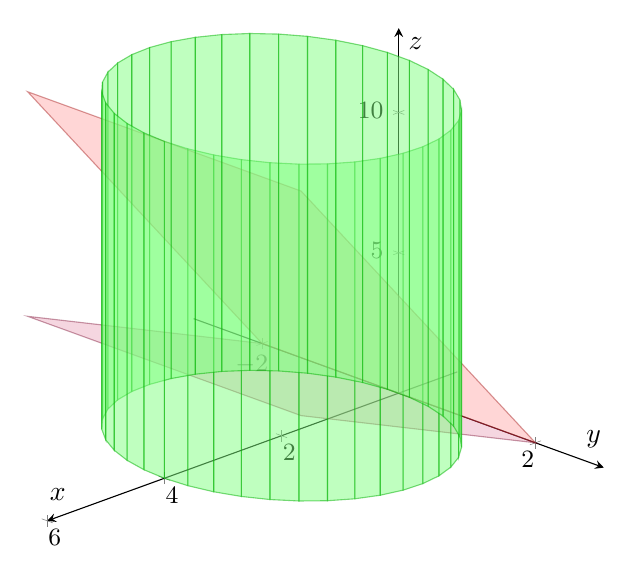
\begin{tikzpicture}
        \begin{axis}[
            view={135}{30}, % Ajustado para ver bien la inclinación de los planos
            width=12cm,
            height=10cm,
            grid=major,
            xmin=-1, xmax=6,
            ymin=-3, ymax=3,
            zmin=0, zmax=13,
            xlabel={$x$},
            ylabel={$y$},
            zlabel={$z$},
            axis lines=center,
            ticklabel style={font=\small},
        ]

        % Plano g: z = x (Violeta)
        \addplot3[
            surf,
            domain=0:4,
            y domain=-2:2,
            samples=2,
            color=purple!40,
            opacity=0.4,
            faceted color=purple!60!black,
        ] {x};

        % Plano h: z = 3x (Rojo)
        \addplot3[
            surf,
            domain=0:4,
            y domain=-2:2,
            samples=2,
            color=red!40,
            opacity=0.4,
            faceted color=red!60!black,
        ] {3*x};

        % Cilindro f: (x-2)^2 + y^2 = 4 (Verde)
        % Parametrización: x = 2 + 2*cos(t), y = 2*sin(t)
        \addplot3[
            surf,
            domain=0:360, % ángulo t
            y domain=0:12, % altura z (hasta el máximo de 3x)
            samples=40,
            samples y=2,
            color=green!50,
            opacity=0.5,
            faceted color=green!70!black,
        ]
        ({2 + 2*cos(x)}, {2*sin(x)}, {y});

        \end{axis}
    \end{tikzpicture}
    \caption{Representación de la región pedida.  \href{https://www.geogebra.org/m/uhgycge3}{Ver en GeoGebra}}
\end{figure}

Para describir la región, utilizamos coordenadas cilíndricas trasladadas:
\[
x = 2 + r\cos\theta, \quad y = r\sin\theta,
\]
con
\[
0 \leq r \leq 2, \qquad 0 \leq \theta \leq 2\pi.
\]

En estas coordenadas, las cotas para \(z\) resultan:
\[
z = 2 + r\cos\theta, \qquad z = 3(2 + r\cos\theta),
\]
es decir,
\[
2 + r\cos\theta \leq z \leq 6 + 3r\cos\theta.
\]

El jacobiano del cambio de variables es
\[
dV = r \, dz \, dr \, d\theta.
\]

Luego, el volumen se expresa como
\[
V = \int_0^{2\pi} \int_0^2 \int_{2 + r\cos\theta}^{6 + 3r\cos\theta} r \, dz \, dr \, d\theta.
\]


\[
V = \int_0^{2\pi} \int_0^2 r \big(4 + 2r\cos\theta\big) \, dr \, d\theta,
\]
\[
V = \int_0^{2\pi} \int_0^2 \big(4r + 2r^2\cos\theta\big) \, dr \, d\theta.
\]

\[
V = \int_0^{2\pi} \left(8 + \frac{16}{3}\cos\theta\right) d\theta.
\]

Finalmente,
\[
\boxed{V = 16\pi}
\]

         
\vspace{0.5 cm}
\begin{example} Calcular el volumen del sólido limitado por la esfera $x^2 + y^2 + z^2 \leq 1$ y el interior del cono $x^2 + y^2 \leq z^2$.
\end{example}

\vspace{0.3cm}
\textbf{Soluci\'on:}
\bigskip
\textbf{Análisis de la región y simetría}

La región $W \subseteq \mathbb{R}^3$ está definida por el interior de la esfera de radio 1 y el interior del cono. Matemáticamente, lo expresamos como:
\[
    W = \{ (x,y,z) \in \mathbb{R}^3 \mid x^2 + y^2 + z^2 \leq 1, \ x^2 + y^2 \leq z^2 \}
\]

\begin{figure}[htbp]
    \centering
    % Llamamos al archivo con el código TikZ extraído
    
    \centering
    \tikzsetnextfilename{ejercicio28_figura} 
    
    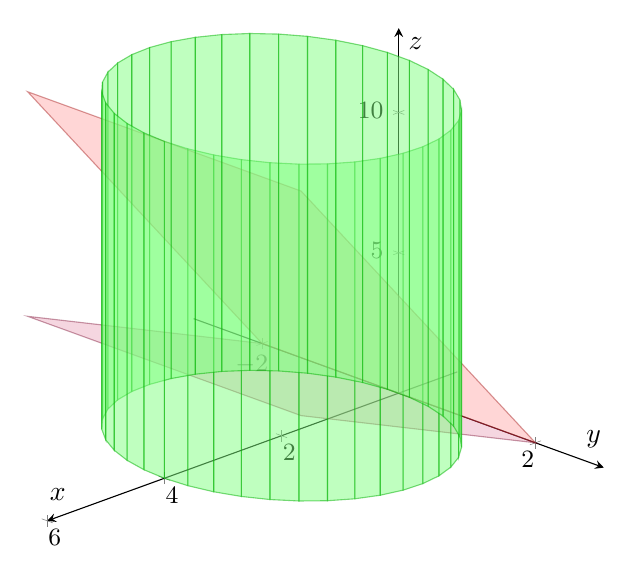
\begin{tikzpicture}
        \begin{axis}[
            view={135}{30}, % Ajustado para ver bien la inclinación de los planos
            width=12cm,
            height=10cm,
            grid=major,
            xmin=-1, xmax=6,
            ymin=-3, ymax=3,
            zmin=0, zmax=13,
            xlabel={$x$},
            ylabel={$y$},
            zlabel={$z$},
            axis lines=center,
            ticklabel style={font=\small},
        ]

        % Plano g: z = x (Violeta)
        \addplot3[
            surf,
            domain=0:4,
            y domain=-2:2,
            samples=2,
            color=purple!40,
            opacity=0.4,
            faceted color=purple!60!black,
        ] {x};

        % Plano h: z = 3x (Rojo)
        \addplot3[
            surf,
            domain=0:4,
            y domain=-2:2,
            samples=2,
            color=red!40,
            opacity=0.4,
            faceted color=red!60!black,
        ] {3*x};

        % Cilindro f: (x-2)^2 + y^2 = 4 (Verde)
        % Parametrización: x = 2 + 2*cos(t), y = 2*sin(t)
        \addplot3[
            surf,
            domain=0:360, % ángulo t
            y domain=0:12, % altura z (hasta el máximo de 3x)
            samples=40,
            samples y=2,
            color=green!50,
            opacity=0.5,
            faceted color=green!70!black,
        ]
        ({2 + 2*cos(x)}, {2*sin(x)}, {y});

        \end{axis}
    \end{tikzpicture}
    \caption{Representación de la región pedida.  \href{https://www.geogebra.org/m/uhgycge3}{Ver en GeoGebra}}
 
    \label{fig:Ejemplo 8.2.5}
\end{figure}

Observamos que el sólido es simétrico respecto al plano $xy$ ($z=0$). Para simplificar el cálculo, trabajaremos únicamente con la mitad superior del sólido (donde $z \geq 0$), a la cual llamaremos $W_s$:
\[
    W_s = \{ (x,y,z) \in \mathbb{R}^3 \mid x^2 + y^2 + z^2 \leq 1, \ x^2 + y^2 \leq z^2, \ z \geq 0 \}
\]

Gracias a dicha simetría podemos calcular el volumen total sabiendo que es el doble del volumen de la región superior: $\text{Vol}(W) = 2 \, \text{Vol}(W_s)$. 

A su vez, de acuerdo con la definición~\ref{def:vol_solido}, el volumen de un sólido se calcula mediante la integral triple de la función constante $1$. Combinando ambas ideas, planteamos:
\[
    \text{Vol}(W) = 2 \iiint_{W_s} 1 \, dV
\]

\textbf{Cambio de variables a coordenadas esféricas \footnote{El planteo completo de este sistema de coordenadas y la deducción de su jacobiano se encuentran disponibles en la sección~\ref{sec:coordenadas_esfericas}.}}  

Para resolver la integral, aplicamos el Teorema~\ref{teo:cambio_variable} utilizando la transformación a esféricas:
\begin{align*}
    x &= \rho \sin \phi \cos \theta \\
    y &= \rho \sin \phi \sin \theta \\
    z &= \rho \cos \phi
\end{align*}

Tal como se demuestra en el ejemplo~\ref{ej:jacobiano_esferico}, el valor absoluto del determinante jacobiano es $|J_{\mathbf{T}}| = \rho^2 \sin \phi$.

\vspace{0.3cm}
\textbf{Nuevos parámetros en $W^*$}

Definimos el conjunto $W^*$ analizando las restricciones sobre nuestra región $W_s$:

\textbf{Rango de $\rho$:} La esfera $x^2 + y^2 + z^2 \leq 1$ define el radio máximo. En esféricas $\rho^2 \leq 1$, por lo tanto $0 \leq \rho \leq 1$.

\textbf{Rango de $\theta$:} El sólido es de revolución completa alrededor del eje $z$. Por lo tanto $0 \leq \theta \leq 2\pi$.

\textbf{Rango de $\phi$ (Triángulo de Intersección):} Buscamos el ángulo máximo donde el cono intercepta a la esfera. Al igualar $x^2 + y^2 = z^2$ con $x^2 + y^2 + z^2 = 1$, obtenemos $2z^2 = 1 \implies z = \frac{1}{\sqrt{2}}$. Este valor de $z$ es nuestro cateto adyacente. El radio del cono en esa altura es el cateto opuesto, que también vale $\sqrt{x^2+y^2} = z = \frac{1}{\sqrt{2}}$.

\begin{figure}[htbp]
    \centering
    % Llamamos al archivo con el código TikZ extraído
    
    \centering
    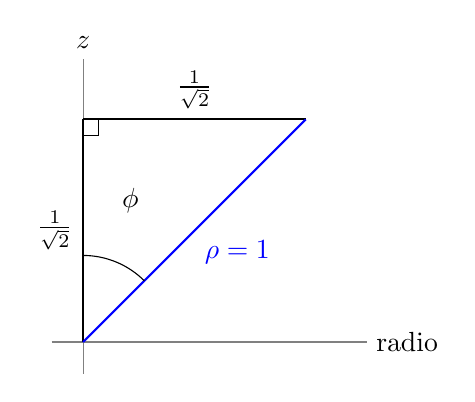
\begin{tikzpicture}[scale=4]
        % Coordenadas
        \coordinate (O) at (0,0); 
        \coordinate (A) at (0,{1/sqrt(2)}); 
        \coordinate (B) at ({1/sqrt(2)},{1/sqrt(2)}); 

        % Ejes tenues
        \draw[gray] (-0.1,0) -- (0.9,0) node[right, black] {radio};
        \draw[gray] (0,-0.1) -- (0,0.9) node[above, black] {$z$};

        % Dibujo del triángulo
        \draw[thick] (O) -- (A) node[midway, left] {$\frac{1}{\sqrt{2}}$}; 
        \draw[thick] (A) -- (B) node[midway, above] {$\frac{1}{\sqrt{2}}$}; 
        \draw[thick, blue] (O) -- (B) node[midway, below right] {$\rho=1$}; 

        % Ángulo recto
        \draw (A) ++(0,-0.05) -- ++(0.05,0) -- ++(0,0.05);

        % Arco de phi interno (Solucionado: dibujado a mano sin depender de librerías)
        \draw (0, 0.275) arc (90:45:0.275);
        \node at (0.15, 0.45) {$\phi$};
    \end{tikzpicture}
 
    \label{fig:triangulo de interseccion}
\end{figure}

Planteamos la relación trigonométrica según el esquema anterior:
\[
    \tan(\phi) = \frac{\text{Cat. Opuesto}}{\text{Cat. Adyacente}} = \frac{1/\sqrt{2}}{1/\sqrt{2}} = 1 \implies \phi = \arctan(1) = \frac{\pi}{4}
\]
    
Como el ángulo nace en el eje $z$ (que es positivo en $W_s$), los límites son $0 \leq \phi \leq \frac{\pi}{4}$.

\vspace{0.3cm}
\textbf{Cálculo del Volumen}

Planteamos primero la integral triple para $W_s$. Debido a que los límites son constantes, podemos separar la expresión en el producto de tres integrales simples:

\[
    \text{Vol}(W_s) = \int_{0}^{2\pi} \int_{0}^{\pi/4} \int_{0}^{1} \rho^2 \sin \phi \, d\rho \, d\phi \, d\theta = \int_{0}^{2\pi} d\theta \int_{0}^{\pi/4} \sin \phi \, d\phi \int_{0}^{1} \rho^2 \, d\rho
\]

Calculamos cada parte de forma independiente:
\[ \int_{0}^{1} \rho^2 \, d\rho = \left[ \frac{\rho^3}{3} \right]_{0}^{1} = \frac{1}{3} \]
\[ \int_{0}^{\pi/4} \sin \phi \, d\phi = \left[ -\cos \phi \right]_{0}^{\pi/4} = -\frac{\sqrt{2}}{2} - (-1) = 1 - \frac{\sqrt{2}}{2} \]
\[ \int_{0}^{2\pi} d\theta = \left[ \theta \right]_{0}^{2\pi} = 2\pi \]

Combinando los resultados parciales y multiplicando por 2 (por la simetría original):
\begin{align*}
    \text{Vol}(W) &= 2 \, \text{Vol}(W_s) \\
    &= 2 \left( 2\pi \right) \left( 1 - \frac{\sqrt{2}}{2} \right) \left( \frac{1}{3} \right) \\
    &= \frac{4\pi}{3} \left( 1 - \frac{\sqrt{2}}{2} \right)
\end{align*}
          

\vspace{0.5 cm}

\begin{example} Calcular $\displaystyle\iiint_{V} \dfrac{1}{y - x - z - 1}\, dx\, dy\, dz$ siendo $V$ el paralelepípedo de caras opuestas
paralelas en el cual tres de sus aristas coinciden con los vectores $(5,2,1),\,(2,4,2),\,(1,3,6)$.
\end{example}

\textbf{Soluci\'on:}
\bigskip

\textbf{1. Análisis de la región de integración $V$}

\medskip

El paralelepípedo $V$ tiene un vértice en el origen y sus tres aristas salientes coinciden con los
vectores $\mathbf{a} = (5,2,1)$, $\mathbf{b} = (2,4,2)$, $\mathbf{c} = (1,3,6)$.

\begin{figure}[htbp]
    \centering
    % Llamamos al archivo con el código TikZ extraído
    
    \centering
    % ESTA LÍNEA es la que crea el PDF en la carpeta /tikz
    \tikzsetnextfilename{ejercicio21_figura} 
    % Colores originales
    \definecolor{zzttqq}{rgb}{0.6,0.2,0}
    \definecolor{ududff}{rgb}{0.30196,0.30196,1}

    \begin{tikzpicture}[line cap=round, line join=round]
    \begin{axis}[
    view={110}{25}, % Ángulo de cámara para perspectiva 3D (azimut y elevación)
    axis lines=center,
    xlabel={$x$}, ylabel={$y$}, zlabel={$z$},
    xmin=-2, xmax=10,
    ymin=-2, ymax=10,
    zmin=-2, zmax=10,
    xtick={-2,2,4,6,8},
    ytick={-2,2,4,6,8},
    ztick={-2,2,4,6,8},
    ticklabel style={font=\scriptsize},
    width=10cm, height=10cm
    ]

    % 1. Definimos los vértices del paralelepípedo en 3D real
    \coordinate (P000) at (0,0,0);
    \coordinate (P100) at (5,2,1); % Vector u
    \coordinate (P010) at (2,4,2); % Vector v
    \coordinate (P001) at (1,3,6); % Vector w

    \coordinate (P110) at (7,6,3); % u + v
    \coordinate (P101) at (6,5,7); % u + w
    \coordinate (P011) at (3,7,8); % v + w
    \coordinate (P111) at (8,9,9); % u + v + w

    % 2. Dibujamos las aristas traseras (ocultas) punteadas
    \draw[very thick, dashed, color=zzttqq] (P000) -- (P010);
    \draw[very thick, dashed, color=zzttqq] (P010) -- (P110);
    \draw[very thick, dashed, color=zzttqq] (P010) -- (P011);

    % 3. Dibujamos las caras visibles (con relleno y opacidad)
    % Cara frontal-derecha
    \filldraw[fill=zzttqq, fill opacity=0.15, draw=zzttqq, very thick] 
    (P000) -- (P100) -- (P101) -- (P001) -- cycle;
    % Cara lateral-derecha
    \filldraw[fill=zzttqq, fill opacity=0.15, draw=zzttqq, very thick] 
    (P100) -- (P110) -- (P111) -- (P101) -- cycle;
    % Cara superior
    \filldraw[fill=zzttqq, fill opacity=0.15, draw=zzttqq, very thick] 
    (P001) -- (P101) -- (P111) -- (P011) -- cycle;

    % 4. Añadimos flechas a los vectores principales
    \draw[very thick, ->, >=Triangle, color=zzttqq] (P000) -- (P100);
    \draw[very thick, dashed, ->, >=Triangle, color=zzttqq] (P000) -- (P010);
    \draw[very thick, ->, >=Triangle, color=zzttqq] (P000) -- (P001);

    % 5. Dibujamos los puntos y etiquetas
    \fill[ududff] (P000) circle (2.5pt); 
    \fill[black!60] (P100) circle (2.5pt); 
    \fill[black!60] (P010) circle (2.5pt); 
    \fill[black!60] (P001) circle (2.5pt); 
    \fill[black!60] (P110) circle (2.5pt); 
    \fill[black!60] (P101) circle (2.5pt); 
    \fill[black!60] (P011) circle (2.5pt); 
    \fill[black!60] (P111) circle (2.5pt); 

    \end{axis}
    \end{tikzpicture}
    \caption{Representación de la región pedida.  \href{https://www.geogebra.org/m/bjnjeat8}{Ver en GeoGebra}}
 
    \label{fig:Ejemplo 8.2.7}
\end{figure}


En coordenadas cartesianas, la región $V$ es difícil de describir directamente, por lo que
recurrimos a un cambio de variables.

\bigskip

\textbf{2. Cambio de variables} \textcolor{red}{Explicar arriba el cambio lineal y referenciar}

\medskip

Definimos la transformación $T: [0,1]^3 \to V$ dada por:
\[
    T(u,v,w) = u\,\mathbf{a} + v\,\mathbf{b} + w\,\mathbf{c},
\]
es decir:
\[
    \begin{cases}
        x = 5u + 2v + w,\\[4pt]
        y = 2u + 4v + 3w,\\[4pt]
        z = \phantom{5}u + 2v + 6w.
    \end{cases}
\]
Al sustituir, la nueva región de integración es el cubo unitario:
\[
    V^* = [0,1] \times [0,1] \times [0,1].
\]

\bigskip

\textbf{3. Jacobiano de la transformación}

\medskip

La matriz jacobiana de $T$ es:
\[
    J_T(u,v,w) =
    \begin{pmatrix}
        \dfrac{\partial x}{\partial u} & \dfrac{\partial x}{\partial v} & \dfrac{\partial x}{\partial w}\\[10pt]
        \dfrac{\partial y}{\partial u} & \dfrac{\partial y}{\partial v} & \dfrac{\partial y}{\partial w}\\[10pt]
        \dfrac{\partial z}{\partial u} & \dfrac{\partial z}{\partial v} & \dfrac{\partial z}{\partial w}
    \end{pmatrix}
    =
    \begin{pmatrix}
        5 & 2 & 1 \\
        2 & 4 & 3 \\
        1 & 2 & 6
    \end{pmatrix}.
\]
Calculando el determinante resulta: $|J_T| = 72$.
\bigskip

\textbf{4. Transformación del integrando}

\medskip

Expresamos $y - x - z - 1$ en las nuevas variables:
\begin{align*}
    y - x - z - 1 &= (2u + 4v + 3w) - (5u + 2v + w) - (u + 2v + 6w) - 1\\
                  &= (2 - 5 - 1)\,u + (4 - 2 - 2)\,v + (3 - 1 - 6)\,w - 1\\
                  &= -4u - 4w - 1.
\end{align*}
Observamos que para $(u,v,w) \in [0,1]^3$ se tiene $-4u - 4w - 1 \in [-9,-1]$,
por lo que el denominador nunca se anula en $V^*$ y la integral está bien definida.

\bigskip

\textbf{5. Cálculo de la integral}

\medskip

Aplicando el Teorema de Cambio de Variables (Teorema 2.5.2):
\begin{align*}
    \iiint_{V} \frac{1}{y-x-z-1}\,dx\,dy\,dz
    &= \iiint_{V^*} \frac{1}{-4u - 4w - 1}\cdot|J_T|\,du\,dv\,dw\\[6pt]
    &= 72\int_0^1\int_0^1\int_0^1 \frac{1}{-4u-4w-1}\,du\,dv\,dw.
\end{align*}

Como el integrando no depende de $v$, la integral en $v$ es trivial:
\[
    = 72\int_0^1\int_0^1 \frac{1}{-4u-4w-1}\,du\,dw.
\]

\textbf{Integral en $u$:}
\begin{align*}
    \int_0^1 \frac{du}{-4u-4w-1}
    &= \left[-\frac{1}{4}\ln\lvert 4u+4w+1\rvert\right]_0^1\\
    &= -\frac{1}{4}\bigl(\ln(4w+5) - \ln(4w+1)\bigr)\\
    &= \frac{1}{4}\ln\!\left(\frac{4w+1}{4w+5}\right).
\end{align*}

\textbf{Integral en $w$:}
\begin{align*}
    \int_0^1 \frac{1}{4}\ln\!\left(\frac{4w+1}{4w+5}\right)dw
    &= \frac{1}{4}\left[\int_0^1\ln(4w+1)\,dw - \int_0^1\ln(4w+5)\,dw\right].
\end{align*}

Para cada integral usamos $\displaystyle\int \ln(4w+a)\,dw = \frac{(4w+a)\ln(4w+a) - (4w+a)}{4}$:

\[
    \int_0^1 \ln(4w+1)\,dw
    = \left[\frac{(4w+1)\bigl(\ln(4w+1)-1\bigr)}{4}\right]_0^1
    = \frac{5(\ln 5 - 1) - 1(\ln 1 - 1)}{4}
    = \frac{5\ln 5 - 4}{4}.
\]

\[
    \int_0^1 \ln(4w+5)\,dw
    = \left[\frac{(4w+5)\bigl(\ln(4w+5)-1\bigr)}{4}\right]_0^1
    = \frac{9(\ln 9 - 1) - 5(\ln 5 - 1)}{4}
    = \frac{9\ln 9 - 5\ln 5 - 4}{4}.
\]

Por lo tanto:
\begin{align*}
    \frac{1}{4}\left[\frac{5\ln 5 - 4}{4} - \frac{9\ln 9 - 5\ln 5 - 4}{4}\right]
    &= \frac{1}{16}\bigl(5\ln 5 - 4 - 9\ln 9 + 5\ln 5 + 4\bigr)\\
    &= \frac{10\ln 5 - 9\ln 9}{16}\\
    &= \frac{10\ln 5 - 18\ln 3}{16}\\
    &= \frac{5\ln 5 - 9\ln 3}{8}.
\end{align*}

Finalmente:
\[
    \iiint_{V} \frac{1}{y-x-z-1}\,dx\,dy\,dz
    = 72 \cdot \frac{5\ln 5 - 9\ln 3}{8}
    = \boxed{9(5\ln 5 - 9\ln 3)}.
\] 
   
   

  \chapter{Superficies en $\mathbb{R}^{3}$ } 
     \section{Superficies parmetrizadas.}
        


\begin{definition}\textbf{Superficie parametrizada}. Sea  $\boldsymbol{\Sigma}:D \subseteq\Rn{2} \to\Rn{3}$ continua y de clase $\mathcal{C}^1(\interior{D})$.  Al conjunto  $S = \text{Img}(\Sigma)$ se lo llama  \emph{superficie}   parametrizada por  $\boldsymbol{\Sigma}$  y   
   a  $\boldsymbol{\Sigma}$  una \emph{parametrizaci\'on} de $S$.
\end{definition}

\begin{obs} Notar que dado un campo escalar $f:D\subset \Rn{2}\to\R$, su gr\'afica  es una superficieparametrizada por  $$ \boldsymbol{\Sigma}:D \subseteq\Rn{2} \to\Rn{3}\: : \: \boldsymbol{\Sigma}(x,y)=(x,y,f(x,y)). $$   
\end{obs}

\begin{example} Sea $f(x,y) = x^2-y^2$. Por la observaci\'on anterior sabemos que la gr\'afica de $f$ es una superficie parametrizada por $\boldsymbol{\Sigma}(x,y)=(x,y,x^2-y^2)$  (podemos pensar a $D = \mathbb{R}^{2}$).  

\vspace{0.3 cm}

\input{figs/sup.tex}
\end{example}

\begin{obs}
Las parametrizaciones de superficies son \'utiles, entre otras cosas,  para describir superficies que no necesariamente son gr\'aficos de una funci\'on. 
\end{obs}

\begin{tarea}\label{parametrizaciones} Hallar una parametrizaci\'on para  las  superficies $S_1$ y $S_2$  dadas por $$S_1=\{ (x,y,z) \in \Rn{3}:  x^{2}+y^{2} =1, \: 0\leq z \leq 3 \},$$ 
$$S_2=\{ (x,y,z) \in \Rn{3}:  x^{2}+y^{2} +z^{2} = 1 \}.$$
\end{tarea}


\begin{definition}\textbf{Superficie regular}. 
 Sea $\boldsymbol{\Sigma}:D\subseteq\Rn{2} \to\Rn{3}$ una parametrizaci\'on de $S$ y sea $(u_0, v_0) \in \interior{D}$.   Diremos que $\boldsymbol{\Sigma}$ es una     
\emph{parametrizaci\'on regular de}  $S$ en  $(u_0, v_0)$  y $S$ una superficie regular en $\boldsymbol{\Sigma}(u_0,v_0)$  si
    \[
       \boldsymbol{\Sigma}_u(u_0,v_0)\times\boldsymbol{\Sigma}(u_0,v_0)\neq \boldsymbol{0}.
   \]
 Si $S$   admite una parametrizaci\'on regular en todo el interior de su dominio diremos que  $S$ es una superficie regular.
 \end{definition}

\begin{obs}\textbf{Idea geom\'etrica}.
\end{obs}

\begin{definition} \textbf{Plano tangente a una  Superficie parametrizada.}  Sea $S$ una superficie parametrizada por $\boldsymbol{\Sigma}:D \subseteq\Rn{2} \to\Rn{3}$ y sea $(u_0,v_0) \in D$. Si $\boldsymbol{\Sigma}$ es regular en $(u_0,v_0)$, se define el plano tangente a $S$ en $\boldsymbol{\Sigma}(u_0,v_0)=(x_0,y_0,z_0)$ al plano $\pi$ dado por la ecuaci\'on
$$\pi: \:\:   \boldsymbol{\Sigma}_u(u_0,v_0)\times\boldsymbol{\Sigma}(u_0,v_0)(x-x_0, y-y_0, z-z_0 )=0$$
\end{definition}

\begin{tarea} Sea $S  \subseteq\Rn{3}$ la superficie parametrizada por  $$\boldsymbol{\Sigma}: [-3,3]\times[-3,3] \to\Rn{3} \:\:\:  \boldsymbol{\Sigma}(u,v)=(u+v,u-v, u^{2}+v^{2}), $$ hallar el plano tangente a $S$ en el punto $(-4,0,8).$  Dibujar en Geogebra el resultado obtenido.   
\end{tarea}


\begin{definition} \textbf{Superficie orientable}.    Sea $S\subseteq\Rn{3}$. Diremos que  $S$  es  \emph{orientable} si existe un campo vectorial  continuo  $\boldsymbol{\eta}:S\to\Rn{3}$ tal que $\boldsymbol{\eta}(\mathbf{p})$ es ortogonal a $S$ en $\mathbf{p}$ y $\norm{\boldsymbol{\eta}(\mathbf{p})}=1\;\forall \mathbf{p}\in S$. Al campo $\boldsymbol{\eta}$ se lo llama \emph{orientaci\'on} de $S$. De no existir un  tal $\boldsymbol{\eta}$ diremos que la superficie es \emph{no orientable}.
\end{definition}


\begin{example} Un ejemplo de una  superficie no orientable es el de una cinta de Möebius. Se deja para el lector profundizar en el tema. 

\vspace{0.3 cm}

\input{figs/moebius.tex}
\end{example}

\begin{obs}
    Si $S$ es una superficie orientable entonces admite dos y solo dos orientaciones. Si  $\boldsymbol{\eta}$  es una orientaci\'on para $S$ entonces  $-\boldsymbol{\eta}$ tambi\'en lo es.
\end{obs}

\begin{definition}\textbf{Orintaci\'on inducida sobre}\label{sigma_induce_1} {\boldmath{$S$}}. Sea $S\subseteq\Rn{3}$ una superficie regular y sea $\boldsymbol{\Sigma}:D\subseteq\Rn{2}\to S$ una parametrizaci\'on continua de clase $\mathcal{C}^1$ y regular de $S$. Lamaremos a  $\boldsymbol{\eta}$ dada por  
\[
            \boldsymbol{\eta}\left(\boldsymbol{\Sigma}(u,v)\right) = \frac{\boldsymbol{\Sigma}_u\times\boldsymbol{\Sigma}_v}{\norm{\boldsymbol{\Sigma}_u\times\boldsymbol{\Sigma}_v}}(u,v) \:\; \forall (u,v) \in D^{0}.
        \]  \emph{ la orientaci\'on inducida} por   $\Sigma$  sobre $S$.  
\end{definition}

\begin{definition}\label{def:preseva} 
    Sea $S\subseteq\Rn{3}$ una superficie regular  orientada por $\boldsymbol{\eta}$ y sea $\boldsymbol{\Sigma}:D\subseteq\Rn{2}\to S$ una parametrizaci\'on continua de clase $\mathcal{C}^1$ y regular de $S$.
    \begin{itemize}
        \item  Decimos que $\boldsymbol{\Sigma}$ \emph{preserva} la orientaci\'on de $S$ si  
        \[
            \frac{\boldsymbol{\Sigma}_u\times\boldsymbol{\Sigma}_v}{\norm{\boldsymbol{\Sigma}_u\times\boldsymbol{\Sigma}_v}}(u,v)=\boldsymbol{\eta}\left(\boldsymbol{\Sigma}(u,v)\right)  \:\; \forall (u,v) \in D^{0}.
        \]  
       
        \item  Decimos que $\boldsymbol{\Sigma}$ \emph{invierte} la orientaci\'on de $S$ si 

 \[
            \frac{\boldsymbol{\Sigma}_u\times\boldsymbol{\Sigma}_v}{\norm{\boldsymbol{\Sigma}_u\times\boldsymbol{\Sigma}_v}}(u,v)=-\boldsymbol{\eta}\left(\boldsymbol{\Sigma}(u,v)\right) \:\: \forall (u,v) \in D^{0}.
        \]
 \end{itemize}
\end{definition}

\begin{tarea} Mostrar la orientaciones inducidas sobre $S_1$ y $S_2$  por sus parametrizaciones  halladas en la \emph{tarea} \ref{parametrizaciones}.
\end{tarea}


\begin{definition} \textbf{Borde de una Superficie.} 
   Sea $\boldsymbol{\Sigma}:D\subseteq\Rn{2} \to\Rn{3}$ una parametrizaci\'on regular  e  inyectiva de una superficie $\boldsymbol{\Sigma}(D) = S$.  Si $ \partial D$,  el borde del conjunto $D$,  es una curva cerrada y simple, se define el \emph{borde}  de $S$, y se lo nota $\partial S$,  a la curva cerrada simple en $\Rn{3}$ tal que 
    \[
        \partial S=\boldsymbol{\Sigma}(\partial D).
    \]
\end{definition}

\begin{definition} \label{sigma_induce} \textbf{Orintaci\'on inducida sobre} {\boldmath{$\partial S$}}.   Sea $\boldsymbol{\Sigma}:D\subseteq\Rn{2} \to\Rn{3}$ una parametrizaci\'on regular  e  inyectiva de una superficie $\boldsymbol{\Sigma}(D) = S$ con $ \partial D$ una curva cerrada y  simple.  Se define  la \emph{orientaci\'on inducida} por  $\boldsymbol{\Sigma}$  sobre  la curva cerrada $\partial S$ a la manera que tiene de recorrer  $\boldsymbol{\Sigma}$ a   $\partial S$,  simpre y cuando se recorra a la curva cerrada y simple $ \partial D \subseteq\Rn{2}$ en sentido antihorario.
\end{definition}

\begin{obs}\label{rmd}\textbf{Regla de la mano derecha.}  En $\Rn{2}$ la orientaci\'on ortogonal de los ejes $x$ e $y$ es \'unica; en cambio en $\Rn{3}$, el tercer eje ortogonal $z$, admite dos posibles 
    orientaci\'ones ``hacia arriba o hacia abajo''. Entonces es necesario definir una convenci\'on para la orientaci\'on de este tercer eje. Dicha convenci\'on es la siguiente: 
    \[
        \vect{i}\times\vect{j}=\vect{k},
    \]  
    donde $\vect{i}$, $\vect{j}$ y $\vect{k}$ son los versores c\'anonicos para los ejes cartesianos $x,\;y,\;z$, respectivamente. Luego \emph{la regla de la mano derecha} es una regla memot\'ecnica que sirve para recordar dicha orientaci\'on.
    \input{figs/mano_derecha.tex}
\end{obs}


\begin{obs}  Sea $\boldsymbol{\Sigma}:D\subseteq\Rn{2} \to\Rn{3}$ una parametrizaci\'on regular  e  inyectiva de una superficie $\boldsymbol{\Sigma}(D) = S$.  La orientaci\'on inducida por $\boldsymbol{\Sigma}$ sobre $S$ (\ref{sigma_induce_1})  y   la orientación inducida por  $\boldsymbol{\Sigma}$  sobre $\partial S$  ( \ref{sigma_induce} ) est\'an relacionadas a trav\'es de la \textbf{Regla de la mano derecha} (\ref{rmd}).
 \end{obs}




%%%%%%%%%%%%%%%%%%%%%%%%%%%%%%%%%%%%%%%%%%%%%%%%%%%%%%%%%%%%%%%%%%%%%%%%%%%%%
%%%%%%%%%%%%%%%%%%%%%%%%%%%%%%%%%%%%%%%%%%%%%%%%%%%%%%%%%%%%%%%%%%%%%%%%%%%%%



 \section{Integrales de Superficie}

\begin{definition}Sea $f:A \subseteq\Rn{3}  \subseteq  \to\mathbb{R}$  un campo continuo y sea $S\subseteq A$ una superficie.  Se define la \emph{ integral de superficie} de $f$ sobre $S$, y se nota  $\iint_S f  \;d\mathbf{S},$ a
    \[
        \iint_S f \;d\mathbf{S}=  \iint_D  f  \circ\boldsymbol{\Sigma}(u,v) \norm{\boldsymbol{\Sigma}_u\times\boldsymbol{\Sigma}_v}(u,v) \;dudv .
    \] donde $\boldsymbol{\Sigma}:D\subseteq\Rn{2} \to\Rn{3}$ una parametrizaci\'on de $S$.
\end{definition} 





\begin{tarea}  Sean  la superficie dada por $S=\{ (x,y,z) \in \Rn{3}:  x^{2}+y^{2} =z, \: 0\leq z \leq 3 \}$ y el campo escalar $f(x,y,z) = x^{2}-y$, calcular  $$   \iint_S f \;d\mathbf{S}. $$
\end{tarea} 


\begin{definition} Sea $S\subseteq \Rn{3}$ una superficie, se define el \emph{ \'area de } $S$, y se nota $A(S)$,  $$A(S) =  \iint_S  1 \;d\mathbf{S}$$
\end{definition}

\begin{tarea} Hallar el \'area de  de las superficies $S_1$ y $S_2$  dadas  en la \emph{tarea} \ref{parametrizaciones}.
\end{tarea}





\begin{definition}
    Sea $S\subseteq\Rn{3}$ una superficie orientada por $\boldsymbol{\eta}$. Sea $\mathbf{F}:A  \subseteq  \to\Rn{3}$  un campo continuo con $S\subset A$. Se define la integral de superficie de $\mathbf{F}$ sobre $S$, (o flujo de $F$ sobre $S$) y se nota  $\iint_S\mathbf{F}\cdot d\mathbf{S},$ a
    \[
        \iint_S \mathbf{F}\;d\mathbf{S}=\iint_S (\mathbf{F}\cdot\boldsymbol{\eta}) \;dS.
    \]
\end{definition} 



\begin{obs}
El producto escalar $\mathbf{F}\cdot\boldsymbol{\eta}$  permite obtener la componente del campo vectorial en la direcci\'on perpendicular a la superficie. Fisicamente, si el campo vectorial se interpreta como un campo de velocidades de un fluido, la integral de superficie puede verse como la \emph{cantidad de fluido} que atraviesa la superficie por unidad de tiempo.
\end{obs}



\begin{tarea}  Sean  la superficie dada por $S=\{ (x,y,z) \in \Rn{3}:  x^{2}+y^{2}  \leq 1, \:  z=1 \}$  y el campo vectorial $F(x,y,z) = (x^{2}+y, z^{2}+y, 2)$, calcular  $$   \iint_S F \cdot \;d\mathbf{S}. $$
\end{tarea} 


\begin{obs}   Sean $S\subseteq\Rn{3}$ una superficie orientada por $\boldsymbol{\eta}$ y  sea  $\boldsymbol{\Sigma}:D\subseteq\Rn{2}\to S\subseteq\Rn{3}$ una parametrizaci\'on de $S$ tal que preserve su orientaci\'on, entonces 
 $$ \iint_S \mathbf{F}\cdot d\mathbf{S} = \iint_D \mathbf{F}\circ\boldsymbol{\Sigma}\cdot\left(\boldsymbol{\Sigma}_u\times\boldsymbol{\Sigma}_v\right)dudv.$$
\end{obs}
Veamos que esto efectivamente es as\'i.  Sabemos que, por la \autoref{def:preseva},
\[
    \frac{\boldsymbol{\Sigma}_u\times\boldsymbol{\Sigma}_v}{\norm{\boldsymbol{\Sigma}_u\times\boldsymbol{\Sigma}_v}}(u,v)=\boldsymbol{\eta}\left(\boldsymbol{\Sigma}(u,v)\right).
\]
Entonces,
\begin{align*}
    \iint_S \mathbf{F}\cdot d\mathbf{S}&=\iint_S (\mathbf{F}\cdot\boldsymbol{\eta}) \;dS = \iint_D (\mathbf{F}\cdot\boldsymbol{\eta})\circ\boldsymbol{\Sigma}(u,v) \:\:\norm{\boldsymbol{\Sigma}_u\times\boldsymbol{\Sigma}_v}(u,v) \;dudv\\[.2cm]
    &=\iint_D (\mathbf{F}\circ\boldsymbol{\Sigma})(u,v) \cdot(\boldsymbol{\eta}\circ\boldsymbol{\Sigma})(u,v) \norm{\boldsymbol{\Sigma}_u\times\boldsymbol{\Sigma}_v}(u,v) \;dudv\\
    &=\iint_D \mathbf{F}\circ\boldsymbol{\Sigma}(u,v) \cdot\left(\boldsymbol{\Sigma}_u\times\boldsymbol{\Sigma}_v\right)(u,v) \: dudv,
\end{align*} concluyendo lo que quer\'iamos ver.

\begin{obs}
    Sea $S$ una superficie con orientaci\'on $\boldsymbol{\eta}$ y sea $\boldsymbol{\Sigma}:D\subseteq\Rn{2}\to S\subseteq\Rn{3}$ una parametrizaci\'on de $S$ tal que invierte su orientaci\'on, entonces
    \[
        \iint_S \mathbf{F}\cdot d\mathbf{S} = \iint_S \mathbf{F}\cdot\eta\;dS=-\iint_D \mathbf{F}\circ\boldsymbol{\Sigma}\cdot(\boldsymbol{\Sigma}_u\times\boldsymbol{\Sigma}_v)\:dudv.
    \]
\end{obs}


\begin{tarea}  Sean  la superficie dada por $S=\{ (x,y,z) \in \Rn{3}:  x^{2}+y^{2} + z^{2} \leq 4, \:  z=1 \}$ y el campo vectorial $F(x,y,z) = (x^{2}+y, z^{2}+y, 2)$, calcular  $$   \iint_S F \cdot \;d\mathbf{S}. $$
\end{tarea} 

\begin{tarea}
 Sea la superficie   $S=\{  (x,y,z) \in \mathbb{R}^{3} \: : \: x ^{2}+ y^{2} = z^{2}, 1 \leq z \leq 2 \}$  y   sea el campo $F(x,y,z)=(x+y^{2}z^{2}, y+z^{2}x^{2}, z).$  Hallar el flujo  de $F$ a trav\'es de $S$ indicando la orientaci\'on elegida.
\end{tarea}  



  


   

  \chapter{Teoremas Integrales }       
       \section{Teoremas Integrales}
            
\begin{theorem} \textbf{Teorema de Green.} \label{green}  Sean $U\subseteq \Rn{2}$ abierto  y   $D \subsetneq  U$ un conjunto  simplemente conexo (\autoref{def:conjuntoconexo_simp}) cuyo borde, $\partial D$, es una curva simple y cerrada.  Si  $\mathbf{F}:U\to\Rn{2}$ es de clase $\mathcal{C}^1$, entonces
    \[
        \oint_{\partial D^{+}} \mathbf{F}\cdot d\mathbf{s} = \iint_D \grad\times\mathbf{F}\cdot d\mathbf{A}.
    \]
\end{theorem}

\begin{obs} Sea $\mathbf{F}:U\subset \Rn{2}\to\Rn{2}$ bajo las condiciones de (\ref{green})  con $\mathbf{F}=(P,Q)$,  el teorema de Green  puede ser escrito de siguiente manera alternativa:
\[
    \oint_{\partial D^+}P\:dx+Q\:dy=\iint_D\left(\dif{Q}{x}-\dif{P}{y}\right)dA,
\]
basta con ver la notaci\'on dada en (\ref{not_int}) y recordar que 
\[
    \nabla\times\mathbf{F} = \dif{Q}{x}-\dif{P}{y}.
\]
\end{obs}

\begin{tarea}
 Para  la curva simple, cerrada y orientada $C$ formada por los segmentos  de $(0, 0)$ a $(1, 1),$ de (1,1) a $(0, 1)$ y de $(0, 1)$ vuelta al $(0, 0)$, calcular  $$\int_{C} xy \; dx + \sqrt{y^{2}+1} \; dy.$$
\end{tarea}


\begin{tarea}
 Sea    $D=\{  (x,y) \in \mathbb{R}^{2} \: : \: 1 \leq x ^{2}+ y^{2}  \leq  4,  x\geq 0 \}$ , calcular   $$\int_{(\partial D)^{-}} x^{2}y \; dx - xy^{2} \; dy.$$
\end{tarea}


\begin{propertie}   Sean $U\subseteq \Rn{2}$ abierto  y   $D \subsetneq  U$ un conjunto  simplemente conexo  cuyo borde, $\partial D$, es una curva simple y cerrada.  Si  $\mathbf{F}:U\to\Rn{2}$ tal que $ \grad\times\mathbf{F} =1 $ entonces
    \[
        \oint_{\partial D^{+}} \mathbf{F}\cdot d\mathbf{s} =  A(D).
    \]
\end{propertie}

\begin{tarea}
Hallar el \'area de la regi\'on encerrada por la curva cerrada con parametrizaci\'on   $\sigma(t) = (\sin t \cos t, \sin t)$ con $0\leq t \leq \pi$.     


 

\begin{figure}[H]
\begin{center}
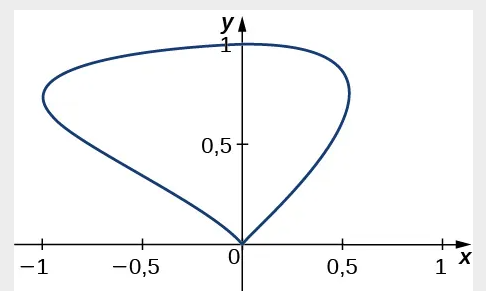
\includegraphics[scale=0.6]{figs/green.png}
\end{center}
\end{figure}
\end{tarea}

\newpage

\begin{obs}
    \textbf{Extensi\'on de Green.} El teorema de Green es aplicable a regiones a\'un m\'as generales que regiones simplemente conexas.  Dicho teorema puede ser adaptado a cualquier regi\'on en $\Rn{2}$ cuya frontera  se pueda descomponer en un n\'umero finito de curvas cerradas y simples.  La idea es ``recorrer" dicha frontera pasando por todas las curvas que la confroman. 

Veamos, a modo ilustrativo,  el siguiente ejemplo. Sea $D \subset \mathbb{R}^{2}$   el siguiente conjunto (pintado de violeta),  claramente $D$  no simplemente conexo. 
    
    \begin{center}
    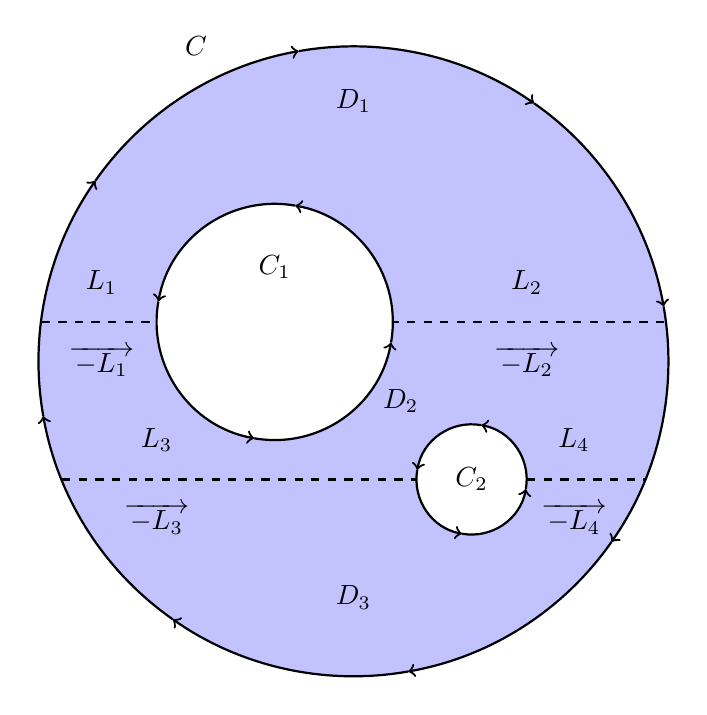
\begin{tikzpicture}
        % Define the exterior boundary with clockwise arrows
        \fill[blue!60!white!40] (0,0) circle (4);
        \foreach \angle in {315, 270, 225, 180, 135, 90, 45, 0} {
            \draw[thick, ->] ({4*cos(\angle+10)}, {4*sin(\angle+10)}) 
                arc[start angle=\angle+10, end angle=\angle-45+10, radius=4];
        }
        
        \draw[thick, dashed] (-3.96, 0.5) -- (3.96, 0.5);
        \draw[thick, dashed] (-3.7, -1.5) -- (3.7, -1.5);
        
        % Inner circle 1 with counterclockwise arrows
        \fill[white] (-1,0.5) circle (1.5);
        \foreach \angle in {0, 90, 180, 270} {
            \draw[thick, ->] ({-1+1.5*cos(\angle+80)}, {0.5+1.5*sin(\angle+80)}) 
            arc[start angle=\angle+80, end angle=\angle+170, radius=1.5];
            }
            
            % Inner circle 2 with counterclockwise arrows
        \fill[white] (1.5,-1.5) circle (0.7);
        \foreach \angle in {0, 90, 180, 270} {
            \draw[thick, ->] ({1.5+0.7*cos(\angle+80)}, {-1.5+0.7*sin(\angle+80)}) 
                arc[start angle=\angle+80, end angle=\angle+170, radius=0.7];
                }

        % Labels for regions
        \node at (0,3.3) {$D_1$};
        \node at (0.6,-0.5) {$D_2$};
        \node at (0,-3) {$D_3$};
        \node at (-2, 4) {$C$};
        \node at (-1,1.2) {$C_1$};
        \node at (1.5,-1.5) {$C_2$};
        \node at (-3.2, 1) {$\underleftarrow{\;\;L_1\;\;}$};
        \node at (-3.2, 0) {$\overrightarrow{\:-L_1\:}$};
        \node at (2.2, 1) {$\underleftarrow{\;\;L_2\;\;}$};
        \node at (2.2, 0) {$\overrightarrow{\:-L_2\:}$};
        \node at (-2.5, -1) {$\underleftarrow{\;\;L_3\;\;}$};
        \node at (-2.5, -2) {$\overrightarrow{\:-L_3\:}$};
        \node at (2.8, -1) {$\underleftarrow{\;\;L_4\;\;}$};
        \node at (2.8, -2) {$\overrightarrow{\:-L_4\:}$};
    \end{tikzpicture}
    \end{center}

El conjunto $D$ puede ser escrito como la uni\'on de tres conjuntos  disjuntos entre si (salvo tal vez en sus bordes) simplemente conexos,  $D_1$, $D_2$ y $D_3$, es decir,  $$D =D_1\cup D_2\cup D_3.$$  El borde de $D$ es la uni\'on de tres curvas cerradas simples,   $C$, $C_1$ y $C_2$, es decir,  $$\partial D=C\cup C_1\cup C_2.$$
Orientemos a la curva  $C$ en sentido horario y a las curvas  $C_1$ y $C_2$  en sentido  antihorario.  

Por lo tanto, si $\mathbf{F}$ es un campo vectorial definido en $D$, aplicando el teorema de Green.
    \begin{align*}
        \oint_{\partial D} \mathbf{F}\cdot d\mathbf{s}=&\oint_{C^{-}}\mathbf{F}\cdot d\mathbf{s}+\oint_{C_1^{+}}\mathbf{F}\cdot d\mathbf{s}+\oint_{C_2^{+}}\mathbf{F}\cdot d\mathbf{s}\\[.2cm]
        =&\oint_{\partial D_1^{-}}\mathbf{F}\cdot d\mathbf{s}+\oint_{\partial D_2^{-}}\mathbf{F}\cdot d\mathbf{s}+\oint_{\partial D_3^{-}}\mathbf{F}\cdot d\mathbf{s}\\[.2cm]
        =&-\iint_{ D_1}\grad\times\mathbf{F}\cdot d\mathbf{A}-\iint_{ D_2}\grad\times\mathbf{F}\cdot d\mathbf{A}-\iint_{ D_3}\grad\times\mathbf{F}\cdot d\mathbf{A}\\[.2cm]
        =&-\iint_D \grad\times\mathbf{F}\cdot d\mathbf{A}
    \end{align*}
\end{obs}

Se deja al lector los detalles del procedimiento anterior. 

\begin{tarea}
Sea $F(x,y) = (\dfrac{y}{x^{2}+y^{2}},\dfrac{-x}{x^{2}+y^{2}})$ y sea $C$ una curva en el plano, cerrada, simple y orientada en sentido antihorario. Calcular todos  los posibles valores de $\int_{C} F ds.$
\end{tarea}


\begin{theorem}
\textbf{Teorema de la divergencia en el plano.} Sea $D\subset\Rn{2}$ una regi\'on donde valga el teorema de Green y sea $\partial D$ su frontera. Denotaremos por $\mathbf{n}$ el versor unitario normal exterior a $\partial D$.  Si $\boldsymbol{\sigma}:[a,b]\to\Rn{2},\;\boldsymbol{\sigma}(t)=(x(t),y(t))$ es una parametrizaci\'on que recorre a $\partial D$ de manera positiva,  entonces  $\mathbf{n}$ est\'a dado por 
\[
    \mathbf{n}=\frac{(y'(t),-x'(t))}{\sqrt{[x'(t)]^2+[y'(t)]^2}}.
\]
Si $\mathbf{F}:  D\to \Rn{2}$ es un campo vectorial continuo y de clase $\mathcal{C}^1(\interior{D})$,  entonces
\[
    \int_{\partial D}\mathbf{F}\cdot\mathbf{n}\:ds=\iint_D\grad\cdot\mathbf{F}\:dA.
\]
\end{theorem}

\begin{theorem}
\textbf{Teorema de Stokes.}  Sean $\boldsymbol{\Sigma}:D\subset\Rn{2} \to S\subset\Rn{3}$    una parametrizaci\'on regular y  de clase  $\mathcal{C}^1(\interior{D})$ de una superficie $S$ y $A \subseteq \Rn{3}$ un conjunto abierto.    Si $\mathbf{F}:  A\subseteq \Rn{3}\to \Rn{3}$ es un campo vectorial continuo, de clase  $\mathcal{C}^1(A)$ tal que  $S \subsetneq A$, entonces
\[
    \oint_{\partial S}\mathbf{F}\cdot d\mathbf{s}=\iint_S\grad\times\mathbf{F}\cdot d\mathbf{S}, 
\]  donde las orientaciones tanto de  $S$ como de $\partial S$ son las inducidas por $\boldsymbol{\Sigma}$ sobre ellas, ver  (\ref{sigma_induce_1}) y  (\ref{sigma_induce}).
\end{theorem}

\begin{tarea} Sean  $S=\{  (x,y,z) \in \mathbb{R}^{3} \: : \:  x ^{2}+ y^{2} = z,  x ^{2}+ y^{2}  \leq 4 \}$  y $F(x,y,z) = (x ^{2}z^{2}, y^{2}z^{2}, xyz)$, calcular, indicando la orientaci\'on elegida   $$\iint_S\grad\times\mathbf{F}\cdot d\mathbf{S}$$
\end{tarea}

\begin{tarea} Sea  $C=\{  (x,y,z) \in \mathbb{R}^{3} \: : \:  z=4, \: x ^{2}+ y^{2}   = 4 \}$  una curva cerrada y simple y sea  $F(x,y,z) = (x ^{3}z^{3}+y, y^{\frac{1}{3}}z^{2}, xyz)$,  calcular,  indicando la orientaci\'on elegida,      $$\int_{C}\mathbf{F}\cdot d\mathbf{S}$$
\end{tarea}



\begin{theorem}
\textbf{Teorema de la divergencia o de Gauss.}  Sean $S\subset\Rn{3}$ una superficie que encierra un volumen $\Omega$, \textit{i.e.} $S=\partial \Omega$, orientada de manera exterior y $A \subseteq \Rn{3}$ un conjunto abierto .  Si $\mathbf{F}:A \subseteq \Rn{3} \to\Rn{3}$ es  un campo vectorial continuo y de clase $\mathcal{C}^1(A)$ tal que $\Omega \subsetneq A$, entonces
\[
    \oiint_{\partial \Omega}\mathbf{F}\cdot d\mathbf{S}=\iiint_{\Omega}\grad\cdot\mathbf{F}\:dV.
\]
\end{theorem}


\begin{tarea}
 Probar que el flujo de $\mathbf{F} = (ax, by, cz)$ con $a,b,c \in \mathbf{R}^+$ a través del cubo: $V : [-1,1] \times [-1,1] \times [-1,1]$ orientado con normales salientes es $(a+b+c) \mathrm{volumen}(V)$.
\end{tarea} 


\begin{tarea}
 Sea la superficie   $S=\{  (x,y,z) \in \mathbb{R}^{3} \: : \: x ^{2}+ y^{2} = z^{2}, 1 \leq z \leq 2 \}$   y   sea el campo $F(x,y,z)=(x+y^{2}z^{2}, y+z^{2}x^{2}, z).$  Hallar el flujo  de $F$ a trav\'es de $S$ indicando la orientaci\'on elegida.
\end{tarea}  



\begin{tarea}
Sea  $S=\{  (x,y,z) \in \mathbb{R}^{3} \: : \: x ^{2}+ y^{2} +1= z,  \:  1\leq z \leq h\}$  y sea  el campo $F(x,y,z)=(z+y^{3},  y+ \cos (z^{2}x^{2}),  -z).$    Hallar $h \in \mathbb{R}$ tal que: $$\int_{S} F . dS = 2\pi. $$  Indicar la orientaci\'on con la cual resuelve el ejercicio.
\end{tarea}


\end{document}   



%===================================================
%               EJERCICIOS RESUELTOS
%===================================================
    \chapter{Ejercicios resueltos}
        \section{Fecha 29 de septiembre de 2023}
            \input{capitulos/1p_29_09_2023}

    
    
        \newpage
        \section{Fecha 25 de abril de 2023}
            \input{capitulos/1p_25_04_2023}





            \newpage
        \section{Fecha 23 de septiembre de 2023}
            \input{capitulos/1P_23_09_2023}


            \newpage
        \section{Fecha 18 de abril de 2024}
            \input{capitulos/1P_18_04_2024}
            


        \newpage
        \section{Fecha Recuperatorio 2cuatri 2022}
            \input{capitulos/1p_recu_2Q_2022}



        \newpage
        \section{Fecha 25 de junio de 2023}
            \input{capitulos/2p_25_06_2023}



        \newpage
        \section{Fecha recuperatorio 29 de junio de 2023}
            \input{capitulos/2p_recu_29_06_2023}



        \newpage
        \section{Fecha 18 de noviembre de 2023}
            \input{capitulos/2p_18_11_2023}



        \newpage
        \section{Fecha 11 de junio de 2024}
            %------------Ejercicio 1---------------------------------------

\begin{question}
    Sean los campos $\psi (x,y) = \ln(\sqrt{x^2+y^2})$ y $\mathbf{F}(x,y)= \left(\psi_y(x,y), -\psi_x(x,y)\right)$
    \\y sea $C$ una curva regular, simple, y cerrada con orientación positiva contenida en el conjunto
    $A=\left\{(x,y): 1 < x^2+y^2 < 9 \right\}$. Hallar los posibles valores de la integral de $\mathbf{F}$ sobre $C$.
\end{question}

%------------Ejercicio 2---------------------------------------

\begin{question}
    Calcular el volumen del cilindro $x^2+y^2 \leq 9$ limitado por el plano $z=-1$ y el
    paraboloide $z=x^2+y^2$.
\end{question}

%------------Ejercicio 3---------------------------------------

\begin{question}
    Calcule el flujo del campo vectorial $\mathbf{F}(x,y,z)= (xz,-y^2,xz)$ a través de la superficie
    $S_1=\left\{x^2+y^2=1 \land 0\leq z \leq 3\right\}$ unión $S_2=\left\{x^2+y^2\leq 1 \land z=0\right\}$.
    Indique gráfica y analíticamente la orientación elegida.
\end{question}


%------------Ejercicio 4---------------------------------------

\begin{question}
    Sea $S$ una superficie en $\mathbb{R}^3$ que encierra un volumen $\Omega$ y sea el campo
    $\mathbf{F}(x,y,z)=(ax,2y,z)$ con $a \in \mathbb{R}$. Hallar $a$ tal que el flujo saliente de $\mathbf{F}$ a través de $S$
    sea igual al volumen de $\Omega$.
\end{question}

%------------Solucion 1---------------------------------------
\newpage
\begin{solution}

    Antes que nada, se debe determinar cuál es la expresión del campo $\mathbf{F}$, en $\mathbb{R}^3-\{(0,0)\}$.
    \begin{align*}
        \psi_x&=\partialx\left(\ln{\sqrt{x^2+y^2}}\right)\\
        &=\frac{1}{\sqrt{x^2+y^2}} \cdot \frac{1}{2\sqrt{x^2+y^2}} \cdot 2x^2\\
        &=\frac{x}{x^2+y^2}
    \end{align*}
    \begin{align*}
        \psi_y&=\partialy\left(\ln{\sqrt{x^2+y^2}}\right)\\
        &=\frac{1}{\sqrt{x^2+y^2}} \cdot \frac{1}{2\sqrt{x^2+y^2}} \cdot 2y^2\\
        &=\frac{y}{x^2+y^2}
    \end{align*}
    \begin{equation*}
        \therefore \mathbf{F}(x,y)= \left(\frac{y}{x^2+y^2}, -\frac{x}{x^2+y^2}\right)
    \end{equation*}
    Para comenzar a resolver el problema, se consideran todas las curvas $C_1$ regulares, simples y cerradas, orientadas positivamente
    y contenidas en $A$ tal que su región encerrada $D_1$, a su vez, también esté contenida en $A$. 
    \begin{center}
        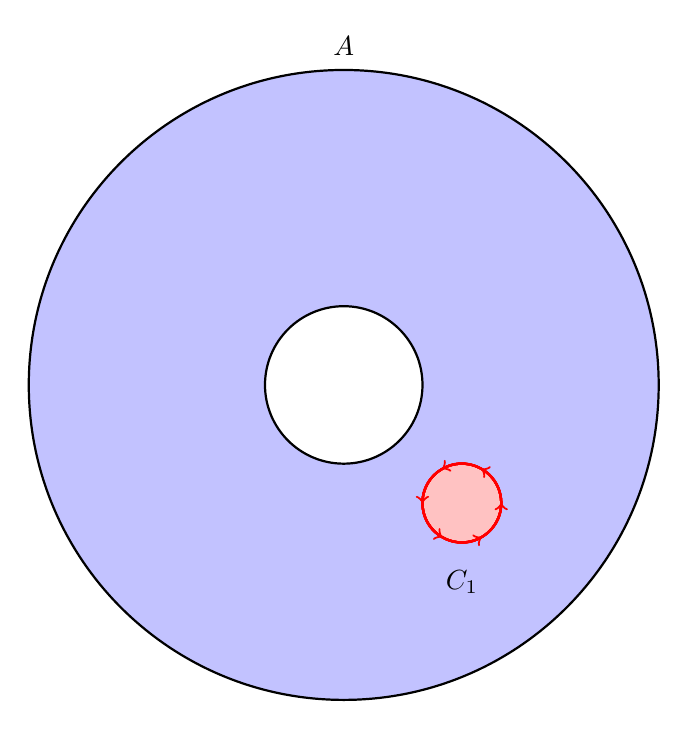
\begin{tikzpicture}
            % Define the exterior boundary
            \draw[thick, fill=blue!60!white!40] (0,0) circle (4);
        
            % Define the inner boundaries
            \draw[thick, fill=white] (0,0) circle (1);

            \draw[thick, red, fill=red!60!white!40] (1.5,-1.5) circle (0.5);
            \foreach \angle in {0, 60, 120, 180, 240, 300} {
                \draw[thick, red, ->] ({1.5+0.5*cos(\angle)}, {-1.5+0.5*sin(\angle)}) arc[start angle=\angle, end angle=\angle+360, radius=0.5];
            }

        
            % Label the regions
            \node at (0,4.3) {$A$};
            \node at (1.5,-2.5) {$C_1$};
            %\node at (0,1.4) {$C_0$};
        
        \end{tikzpicture}
    \end{center}
    En este caso, con $boldsymbol{F}$ una función de clase
    $\mathcal{C}^1$ en $A$, valen las hipótesis del teorema de Green (tanto para la curva como para el campo). Entonces:
    \begin{equation*}
        \int_{C_1}\mathbf{F}\cdot d\boldsymbol{s} = \iint_{D_1}\left(\grad \times \mathbf{F}\right)dA
    \end{equation*}
    Acto siguiente, se calcula el rotor de $\mathbf{F}$, para resolver la integral.
    \begin{align*}
        \grad \times \mathbf{F} &= \partialx\left( -\frac{x}{x^2+y^2}\right) - \partialy\left(\frac{y}{x^2+y^2}\right)\\
        &= \left(-\frac{(x^2+y^2)-2x^2}{\left(x^2+y^2\right)^2}\right) - \left(\frac{(x^2+y^2)-2y^2}{\left(x^2+y^2\right)^2}\right)\\
        &= -\left(\frac{-x^2+y^2}{\left(x^2+y^2\right)^2}+\frac{x^2-y^2}{\left(x^2+y^2\right)^2}\right)\\
        &= -\left(\frac{-x^2+y^2+x^2-y^2}{\left(x^2+y^2\right)^2}\right)\\
        \grad \times \mathbf{F}&= 0
    \end{align*}
    Por lo tanto, la integral del campo sobre $C_1$ resulta:
    \begin{align*}
        \int_{C_1}\mathbf{F}\cdot d\boldsymbol{s} &= \iint_{D_1}\left(0\right)dA\\
        \Rightarrow \int_{C_1}\mathbf{F}\cdot d\boldsymbol{s} &= 0
    \end{align*}
    Ahora queda considerar los casos de todas las curvas $C_2$ regulares, simples y cerradas, orientadas positivamente
    y contenidas en $A$ tal que su región encerrada $D_2$ no esté totalmente contenida dentro de $A$.
    \begin{center}
        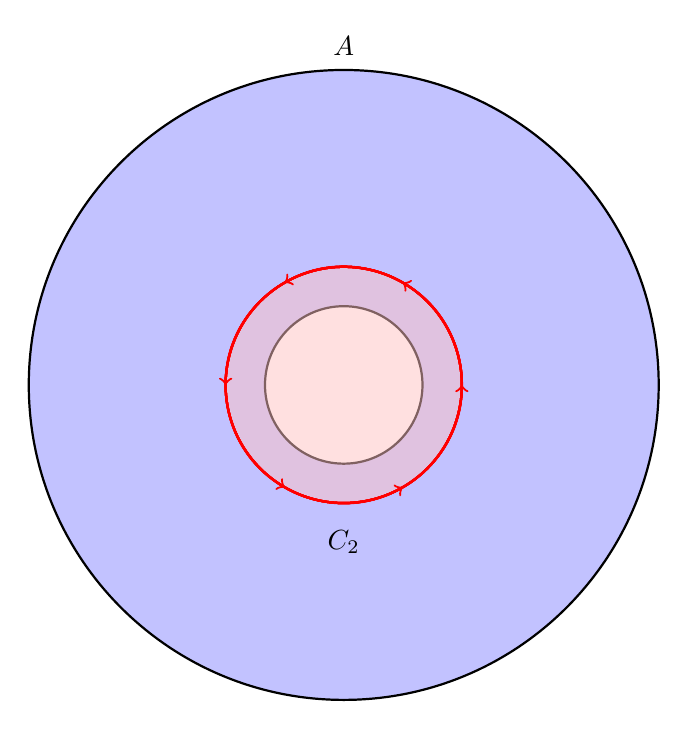
\begin{tikzpicture}
            % Define the exterior boundary
            \draw[thick, fill=blue!60!white!40] (0,0) circle (4);
        
            % Define the inner boundaries
            \draw[thick, fill=white] (0,0) circle (1);

            \draw[thick, red, fill=red!60!white!40, opacity=0.5] (0,0) circle (1.5);
            \foreach \angle in {0, 60, 120, 180, 240, 300} {
                \draw[thick, red, ->] ({1.5*cos(\angle)}, {1.5*sin(\angle)}) arc[start angle=\angle, end angle=\angle+360, radius=1.5];
            }

        
            % Label the regions
            \node at (0,4.3) {$A$};
            \node at (0,-2) {$C_2$};
            %\node at (0,1.4) {$C_0$};
        
        \end{tikzpicture}
    \end{center}
    En este caso, ya no se cumplen las condiciones del teorema de Green, puesto que $\mathbf{F}$ no se encuentra definida en $(0,0) \in D_2$.
    Sin embargo, es posible utilizar el teorema de Green generalizado. Definiendo previamente, con orientación positiva:
    \begin{align*}
        C_0&=\left\{(x,y): x^2+y^2=1 \right\}\\
        C_0&=\partial D_0
    \end{align*}
    \begin{center}
        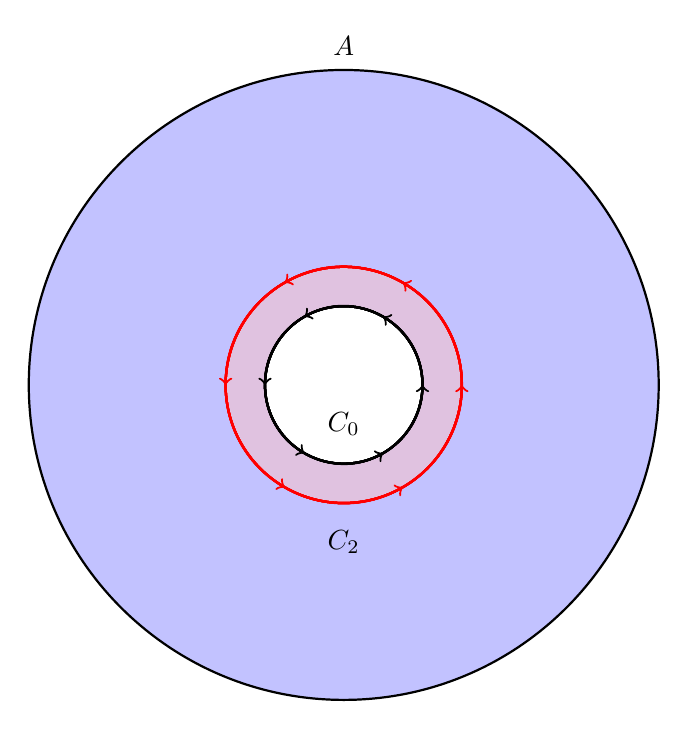
\begin{tikzpicture}
            % Define the exterior boundary
            \draw[thick, fill=blue!60!white!40] (0,0) circle (4);
        
            \draw[thick, red, fill=red!60!white!40, opacity=0.5] (0,0) circle (1.5);
            \foreach \angle in {0, 60, 120, 180, 240, 300} {
                \draw[thick, red, ->] ({1.5*cos(\angle)}, {1.5*sin(\angle)}) arc[start angle=\angle, end angle=\angle+360, radius=1.5];
            }

            % Define the inner boundaries
            \draw[thick, fill=white] (0,0) circle (1);
            \foreach \angle in {0, 60, 120, 180, 240, 300} {
                \draw[thick, ->] ({cos(\angle)}, {sin(\angle)}) arc[start angle=\angle, end angle=\angle+360, radius=1];
            }


        
            % Label the regions
            \node at (0,4.3) {$A$};
            \node at (0,-2) {$C_2$};
            \node at (0,-0.5) {$C_0$};
        
        \end{tikzpicture}
    \end{center}
    Luego, se puede utlizar el teorema de Green generalizado:
    \begin{equation*}
        \int_{C_2}\mathbf{F}\cdot d\boldsymbol{s} - \int_{C_0}\mathbf{F}\cdot d\boldsymbol{s} = \iint_{\left(D_2-D_0\right)}\left(\grad \times \mathbf{F}\right)dA
    \end{equation*}
    Sobre el área entre ambas curvas, el rotor del campo vale cero, puesto que está definido en $\left(D_2-D_0\right)\subset A$. Entonces, el término de la derecha, se vuelve cero.
    \begin{equation*}
        \int_{C_2}\mathbf{F}\cdot d\boldsymbol{s} = \int_{C_0}\mathbf{F}\cdot d\boldsymbol{s}
    \end{equation*}
    Para realizar la integral de la derecha, se propone la parametrización:
    \begin{equation*}
        \sigma: B=[0;2\pi] \longrightarrow \mathbb{R}^2 / \sigma(t) = (\cos(t),\sin(t))
    \end{equation*}
    \begin{equation*}
        \sigma'(t)=(-\sin(t),\cos(t))
    \end{equation*}
    Por lo tanto:
    \begin{align*}
        \int_{C_0}\mathbf{F}\cdot d\boldsymbol{s}&=\int_{0}^{2\pi}\mathbf{F}\circ\sigma(t) \cdot \sigma'(t) dt\\
        &=\int_{0}^{2\pi} (\sin(t),-\cos(t)) \cdot (-\sin(t),\cos(t)) dt\\
        &=\int_{0}^{2\pi} \left(-\sin^2(t)-\cos^2(t)\right) dt\\
        &=\int_{0}^{2\pi} -\left(\sin^2(t)+\cos^2(t)\right) dt\\
        &=-\int_{0}^{2\pi} 1 dt\\
        &=-\left.\left(t\right)\right|_{0}^{2\pi}\\
        \int_{C_0}\mathbf{F}\cdot d\boldsymbol{s}&=-2\pi\\
        \Rightarrow \int_{C_2}\mathbf{F}\cdot d\boldsymbol{s}&=-2\pi
    \end{align*}
\end{solution}

%------------Solucion 2---------------------------------------

\begin{solution}
    Primero, se debe determinar el volumen a calcular como un conjunto elemental, para poder
    realizar la integral. La primera condición del volumen, es que $x^2+y^2 \leq 9$. Luego, quedaría restringir
    en qué intervalo se encuentra el valor de $z$.
    
    Uno de los límites, como lo dice la consigna es $z=-1$.
    El otro límite es, entonces, la superficie $z=x^2+y^2$. Graficarlos nota claramente que la superficie
    descripta por el paraboloide se encuentra sobre el plano $z=-1$. Por lo tanto, la restricción para es
    $-1\leq z \leq x^2+y^2$. También se puede razonar que $0\leq x^2+y^2$ por lo que la $z=-1 < 0 \leq z=x^2+y^2$.

    Para expresar el conjunto elemental conviene hacerlo, en coordenadas cilíndricas, con $x^2+y^2=\rho^2$:
    \begin{equation*}
        \Omega = \left\{(\rho,\phi,z) \in \mathbb{R}^3 : 0\leq\rho\leq 3 \land -1\leq z \leq \rho \land 0\leq\phi\leq 2\pi \right\}
    \end{equation*}
    Ahora sí, se puede calcular el volumen en coordenadas cilíndricas:
    \begin{align*}
        \text{Vol}(\Omega)&=\iiint_\Omega dV\\
        &=\iiint_\Omega dxdydz\\
        &=\iiint_\Omega \rho d\phi dz d\rho\\
        &= \int_0^3 \int_{-1}^{\rho^2} \int_0^{2\pi} \rho d\phi dz d\rho\\
        &= \int_0^3 \int_{-1}^{\rho^2} \rho \left.\phi\right|_{\phi=0}^{\phi=2\pi} dz d\rho\\
        &= \int_0^3 \int_{-1}^{\rho^2} \rho \cdot 2\pi \cdot dz d\rho\\
        &= 2\pi \cdot \int_0^3 \rho \left.z\right|_{z=-1}^{z=\rho^2} d\rho\\
        &= 2\pi \cdot \int_0^3 \rho \left(\rho^2+1\right) d\rho\\
        &= 2\pi \cdot \int_0^3 \left(\rho^3+\rho\right) d\rho\\
        &= 2\pi \cdot \left.\left(\frac{\rho^4}{4}+\frac{\rho^2}{2}\right)\right|_{\rho=0}^{\rho=3}\\
        \therefore\text{Vol}(\Omega)&= \frac{99}{2}\pi
    \end{align*}

\end{solution}
%------------Solucion 3---------------------------------------

\begin{solution}
    Para entender el problema, primero grafiquemos las superficies.
    \begin{center}
        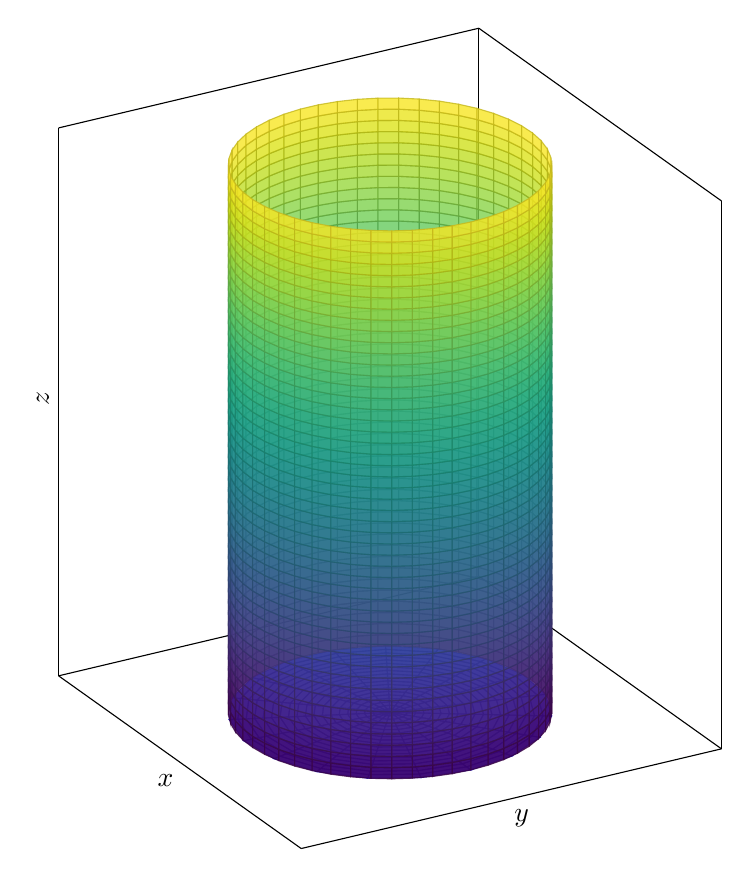
\begin{tikzpicture}
            \begin{axis}[
                    view={60}{20},
                    xlabel=$x$,
                    ylabel=$y$,
                    zlabel=$z$,
                    xmin=-1.5,
                    ymin=-1.5,
                    zmin=0,
                    xmax=1.5,
                    ymax=1.5,
                    zmax=3,
                    width=10cm,
                    height=12cm,
                    ticks=none
                ]

                % Base del cilindro (Disco sólido en z=0)
                % x = radio (0 a 1), y = ángulo (0 a 360)
                \addplot3 [surf, domain=0:1, y domain=0:360, samples=20, fill=blue, draw=none, opacity=0.8] 
                ({x*cos(y)}, {x*sin(y)}, {0});
                
                % Paredes del cilindro
                % x = ángulo (0 a 360), y = altura z (0 a 3)
                \addplot3 [surf, opacity=0.8, draw=none, domain=0:360, y domain=0:3, samples=50, colormap/viridis] 
                ({cos(x)}, {sin(x)}, {y});   

            \end{axis}
        \end{tikzpicture}
    \end{center}
    Se trata de una superficie cilíndrica, con una tapa inferior en $z=0$, pero no una tapa superior en $z=3$.
    Para calcular entonces el flujo de $\mathbf{F}$ habría, en principio, que parametrizar la superficie cilíndrica y la
    tapa por separadas, y luego calcular dos integrales, una por cada superficie.

    Sin embargo, si se le agrega a estas dos superficies una tercera $S_T$, que sea la tapa superior del cilindro.
    Así $S_C = S_1 \bigcup S_2 \bigcup S_T$ encierra el volumen del cilindro ($\Omega$). Esta superficie $S_C = \partial\Omega$, si se
    orienta de saliente, cumple las condiciones del teorema de la divergencia. Con $\mathbf{F} \in \mathcal{C}^1$:
    \begin{align*}
        \iint_{S_C} \mathbf{F} \cdot d\boldsymbol{S} &= \iiint_{\Omega} \grad \cdot \mathbf{F} dV\\
        \iint_{S_1 \bigcup S_2} \mathbf{F} \cdot d\boldsymbol{S} + \iint_{S_T} \mathbf{F} \cdot d\boldsymbol{S}&= \iiint_{\Omega} \grad \cdot \mathbf{F} dV\\
        \iint_{S_1 \bigcup S_2} \mathbf{F} \cdot d\boldsymbol{S} &= \iiint_{\Omega} \grad \cdot \mathbf{F} dV - \iint_{S_T} \mathbf{F} \cdot d\boldsymbol{S}
    \end{align*}
    Ahora, se deben calcular las dos integrales del miembro derecho. Para la primera, se debe representar el $\Omega$ 
    como un conjunto elemental, lo que resulta fácil en coordenadas cilíndricas:
    \begin{equation*}
    \Omega = \left\{(\rho,\phi,z) \in \mathbb{R}^3: 0\leq\rho\leq1 \land 0\leq\phi\leq2\pi \land 0\leq z \leq 3 \right\}
    \end{equation*}
    Por lo tanto:
    \begin{align*}
        \iiint_{\Omega} \grad \cdot \mathbf{F} dV &= \iiint_{\Omega} \left(z-2y+x\right)dxdydz\\
        &=\iiint_{\Omega} \left(z-2\rho\sin{\phi}+\rho\cos{\phi}\right)\rho d\phi dz d\rho\\
        &=\int_{0}^{1} \int_{0}^{3} \int_{0}^{2\pi} \left(z\rho-2\rho^2\sin{\phi}+\rho^2\cos{\phi}\right) d\phi dz d\rho\\
        &= \int_{0}^{1} \int_{0}^{3}  \left.\left(z\rho\phi+2\rho^2\cos{\phi}+\rho^2\sin{\phi}\right)\right|_{\phi=0}^{\phi=2\pi} dz d\rho\\
        &= \int_{0}^{1} \int_{0}^{3}  \left(z\rho\cdot2\pi\right) dz d\rho\\
        &= \pi\int_{0}^{1}  \left.\left(z^2\rho\right)\right|_{z=0}^{z=3} d\rho\\
        &= \pi\int_{0}^{1}  \left(9\rho\right) d\rho\\
        &= 9\pi \left.\left(\frac{\rho^2}{2}\right)\right|_{\rho=0}^{\rho=1}\\
        \iiint_{\Omega} \grad \cdot \mathbf{F} dV&= \frac{9}{2}\pi
    \end{align*}
    Para la segunda integral a resolver, primero es necesaria la parametrización de $S_T$. Para ello, se propone 
    $D=\left\{(\rho,\phi) \in \mathbb{R}^2 : 0\leq\rho\leq1 \land 0\leq\phi\leq2\pi\right\}$ y la parametrización:
    \begin{equation*}
        \boldsymbol{\Sigma} : D \subset \mathbb{R}^2 \longrightarrow \mathbb{R}^3 / \boldsymbol{\Sigma}(\rho,\phi) = \left(\rho\cos{\phi},\rho\sin{\phi},3\right)
    \end{equation*}
    tal que $\boldsymbol{\Sigma_{\rho}}\times\boldsymbol{\Sigma_{\phi}} = \left(0,0,\rho\right)$, con $\rho>0$ orienta la superficie saliente, como se había definido previamente.
    Luego, ya es posible calcular la integral:
    \begin{align*}
        \iint_{S_T} \mathbf{F} \cdot d\boldsymbol{S} &= \iint_{D} (3\rho\cos{\phi},-\rho^2\sen^2{\phi},3\rho\cos{\phi}) \cdot (0,0,\rho)dA\\
        &= \iint_{D} 3\rho^2\cos{\phi}dA\\
        &= \int_{0}^{1} \int_{0}^{2\pi} 3\rho^2\cos{\phi} d\phi d\rho\\
        &= \int_{0}^{1} 3\rho^2\left.\sin{\phi}\right|_{\phi=0}^{\phi=2\pi} d\rho \\
        &= \int_{0}^{1} 3\rho^2\cdot 0 \cdot d\rho\\
        \iint_{S_T} \mathbf{F} \cdot d\boldsymbol{S} &= 0 \\
    \end{align*}
    Con estos dos resultados, ya es posible calcular la integral que pide la consigna, recordando que la orientación de las superficies se definió saliente.
    \begin{align*}
        \iint_{S_1 \bigcup S_2} \mathbf{F} \cdot d\boldsymbol{S} &= \iiint_{\Omega} \grad \cdot \mathbf{F} dV - \iint_{S_T} \mathbf{F} \cdot d\boldsymbol{S}\\
        &= \frac{9}{2}\pi - 0\\
        \therefore \iint_{S_1 \bigcup S_2} \mathbf{F} \cdot d\boldsymbol{S} &= \frac{9}{2}\pi
    \end{align*}
\end{solution}

%------------Solucion 4---------------------------------------

\begin{solution}
    Primero, notemos que la el campo $\mathbf{F}$ es un campo $\mathcal{C}^1(\mathbb{R}^3)$, puesto que
    cada una de sus componentes lo es, independientemente del valor de $a \in \mathbb{R}$.
    Por lo tanto, con $S = \partial \Omega$ orientada saliente, se cumplen las hipótesis del
    teorema de la divergencia, tal que:
    \begin{equation*}
        \iint_S \mathbf{F} \cdot d\boldsymbol{S} = \iiint_\Omega \grad \cdot \mathbf{F} dV
    \end{equation*}
    Por lo tanto, la condición que plantea la consigna:
    \begin{equation*}
        \iint_S \mathbf{F} \cdot d\boldsymbol{S} = \text{Vol}(\Omega)
    \end{equation*}
    se puede reescribir como:
    \begin{equation*}
        \iiint_\Omega \grad \cdot \mathbf{F} dV = \iiint_\Omega dV
    \end{equation*}
    Para que se cumple lo anterior, es suficiente con pedir que la divergencia del campo resulte $1$.
    \begin{align*}
        \grad \cdot \mathbf{F} &= 1 \\
        \partialx(ax) + \partialy(2y) + \partialz(z) &= 1 \\
        a + 2 + 1 &= 1 \\
        \therefore a &= -2
    \end{align*}
\end{solution}
     
    
      %  \newpage
        %\section{Fecha 28 de septiembre de 2024}  Hay algun problrma de compilacion
           % \input{capitulos/1P_28_09_2024}
          
           
            
       % \newpage
        %\section{Fecha 11 de noviembre de 2024} Hay algun problrma de compilacion
           % \input{capitulos/2P_11_11_2024}
          
                  \newpage
        \section{Fecha recuperatorio extra}
            \input{capitulos/2doRecupExtra}
    
 \end{document}  
